\documentclass[twoside]{book}

% Packages required by doxygen
\usepackage{fixltx2e}
\usepackage{calc}
\usepackage{doxygen}
\usepackage[export]{adjustbox} % also loads graphicx
\usepackage{graphicx}
\usepackage[utf8]{inputenc}
\usepackage{makeidx}
\usepackage{multicol}
\usepackage{multirow}
\PassOptionsToPackage{warn}{textcomp}
\usepackage{textcomp}
\usepackage[nointegrals]{wasysym}
\usepackage[table]{xcolor}

% Font selection
\usepackage[T1]{fontenc}
\usepackage[scaled=.90]{helvet}
\usepackage{courier}
\usepackage{amssymb}
\usepackage{sectsty}
\renewcommand{\familydefault}{\sfdefault}
\allsectionsfont{%
  \fontseries{bc}\selectfont%
  \color{darkgray}%
}
\renewcommand{\DoxyLabelFont}{%
  \fontseries{bc}\selectfont%
  \color{darkgray}%
}
\newcommand{\+}{\discretionary{\mbox{\scriptsize$\hookleftarrow$}}{}{}}

% Page & text layout
\usepackage{geometry}
\geometry{%
  a4paper,%
  top=2.5cm,%
  bottom=2.5cm,%
  left=2.5cm,%
  right=2.5cm%
}
\tolerance=750
\hfuzz=15pt
\hbadness=750
\setlength{\emergencystretch}{15pt}
\setlength{\parindent}{0cm}
\setlength{\parskip}{3ex plus 2ex minus 2ex}
\makeatletter
\renewcommand{\paragraph}{%
  \@startsection{paragraph}{4}{0ex}{-1.0ex}{1.0ex}{%
    \normalfont\normalsize\bfseries\SS@parafont%
  }%
}
\renewcommand{\subparagraph}{%
  \@startsection{subparagraph}{5}{0ex}{-1.0ex}{1.0ex}{%
    \normalfont\normalsize\bfseries\SS@subparafont%
  }%
}
\makeatother

% Headers & footers
\usepackage{fancyhdr}
\pagestyle{fancyplain}
\fancyhead[LE]{\fancyplain{}{\bfseries\thepage}}
\fancyhead[CE]{\fancyplain{}{}}
\fancyhead[RE]{\fancyplain{}{\bfseries\leftmark}}
\fancyhead[LO]{\fancyplain{}{\bfseries\rightmark}}
\fancyhead[CO]{\fancyplain{}{}}
\fancyhead[RO]{\fancyplain{}{\bfseries\thepage}}
\fancyfoot[LE]{\fancyplain{}{}}
\fancyfoot[CE]{\fancyplain{}{}}
\fancyfoot[RE]{\fancyplain{}{\bfseries\scriptsize Generated by Doxygen }}
\fancyfoot[LO]{\fancyplain{}{\bfseries\scriptsize Generated by Doxygen }}
\fancyfoot[CO]{\fancyplain{}{}}
\fancyfoot[RO]{\fancyplain{}{}}
\renewcommand{\footrulewidth}{0.4pt}
\renewcommand{\chaptermark}[1]{%
  \markboth{#1}{}%
}
\renewcommand{\sectionmark}[1]{%
  \markright{\thesection\ #1}%
}

% Indices & bibliography
\usepackage{natbib}
\usepackage[titles]{tocloft}
\setcounter{tocdepth}{3}
\setcounter{secnumdepth}{5}
\makeindex

% Hyperlinks (required, but should be loaded last)
\usepackage{ifpdf}
\ifpdf
  \usepackage[pdftex,pagebackref=true]{hyperref}
\else
  \usepackage[ps2pdf,pagebackref=true]{hyperref}
\fi
\hypersetup{%
  colorlinks=true,%
  linkcolor=blue,%
  citecolor=blue,%
  unicode%
}

% Custom commands
\newcommand{\clearemptydoublepage}{%
  \newpage{\pagestyle{empty}\cleardoublepage}%
}

\usepackage{caption}
\captionsetup{labelsep=space,justification=centering,font={bf},singlelinecheck=off,skip=4pt,position=top}

%===== C O N T E N T S =====

\begin{document}

% Titlepage & ToC
\hypersetup{pageanchor=false,
             bookmarksnumbered=true,
             pdfencoding=unicode
            }
\pagenumbering{alph}
\begin{titlepage}
\vspace*{7cm}
\begin{center}%
{\Large C\+Engine \\[1ex]\large 0.\+1 }\\
\vspace*{1cm}
{\large Generated by Doxygen 1.8.13}\\
\end{center}
\end{titlepage}
\clearemptydoublepage
\pagenumbering{roman}
\tableofcontents
\clearemptydoublepage
\pagenumbering{arabic}
\hypersetup{pageanchor=true}

%--- Begin generated contents ---
\chapter{Hierarchical Index}
\section{Class Hierarchy}
This inheritance list is sorted roughly, but not completely, alphabetically\+:\begin{DoxyCompactList}
\item \contentsline{section}{ce\+:\+:core\+:\+:Application}{\pageref{classce_1_1core_1_1_application}}{}
\item \contentsline{section}{ce\+:\+:graphics\+:\+:Base\+Light}{\pageref{classce_1_1graphics_1_1_base_light}}{}
\begin{DoxyCompactList}
\item \contentsline{section}{ce\+:\+:graphics\+:\+:Dir\+Light}{\pageref{classce_1_1graphics_1_1_dir_light}}{}
\item \contentsline{section}{ce\+:\+:graphics\+:\+:Point\+Light}{\pageref{classce_1_1graphics_1_1_point_light}}{}
\item \contentsline{section}{ce\+:\+:graphics\+:\+:Spot\+Light}{\pageref{classce_1_1graphics_1_1_spot_light}}{}
\end{DoxyCompactList}
\item \contentsline{section}{ce\+:\+:graphics\+:\+:Camera}{\pageref{classce_1_1graphics_1_1_camera}}{}
\item \contentsline{section}{ce\+:\+:core\+:\+:Clock}{\pageref{classce_1_1core_1_1_clock}}{}
\item \contentsline{section}{ce\+:\+:core\+:\+:Input}{\pageref{classce_1_1core_1_1_input}}{}
\item \contentsline{section}{ce\+:\+:core\+:\+:Joystick}{\pageref{structce_1_1core_1_1_joystick}}{}
\item \contentsline{section}{ce\+:\+:graphics\+:\+:Light\+Setup}{\pageref{structce_1_1graphics_1_1_light_setup}}{}
\item \contentsline{section}{ce\+:\+:graphics\+:\+:Material}{\pageref{structce_1_1graphics_1_1_material}}{}
\item \contentsline{section}{ce\+:\+:graphics\+:\+:Mesh}{\pageref{classce_1_1graphics_1_1_mesh}}{}
\item \contentsline{section}{ce\+:\+:graphics\+:\+:Model}{\pageref{classce_1_1graphics_1_1_model}}{}
\item \contentsline{section}{ce\+:\+:graphics\+:\+:Model\+Loader}{\pageref{classce_1_1graphics_1_1_model_loader}}{}
\item \contentsline{section}{ce\+:\+:graphics\+:\+:Render\+Command}{\pageref{structce_1_1graphics_1_1_render_command}}{}
\item \contentsline{section}{ce\+:\+:graphics\+:\+:Renderer3D}{\pageref{classce_1_1graphics_1_1_renderer3_d}}{}
\begin{DoxyCompactList}
\item \contentsline{section}{ce\+:\+:graphics\+:\+:Forward\+Renderer}{\pageref{classce_1_1graphics_1_1_forward_renderer}}{}
\end{DoxyCompactList}
\item \contentsline{section}{ce\+:\+:graphics\+:\+:Shader}{\pageref{classce_1_1graphics_1_1_shader}}{}
\item \contentsline{section}{ce\+:\+:graphics\+:\+:Shader\+Loader}{\pageref{classce_1_1graphics_1_1_shader_loader}}{}
\item \contentsline{section}{ce\+:\+:graphics\+:\+:Shader\+Properties}{\pageref{structce_1_1graphics_1_1_shader_properties}}{}
\item \contentsline{section}{ce\+:\+:graphics\+:\+:Texture}{\pageref{structce_1_1graphics_1_1_texture}}{}
\item \contentsline{section}{ce\+:\+:core\+:\+:Time}{\pageref{structce_1_1core_1_1_time}}{}
\item \contentsline{section}{ce\+:\+:graphics\+:\+:Vertex}{\pageref{structce_1_1graphics_1_1_vertex}}{}
\item \contentsline{section}{ce\+:\+:core\+:\+:Window}{\pageref{classce_1_1core_1_1_window}}{}
\end{DoxyCompactList}

\chapter{Class Index}
\section{Class List}
Here are the classes, structs, unions and interfaces with brief descriptions\+:\begin{DoxyCompactList}
\item\contentsline{section}{\hyperlink{classce_1_1core_1_1_application}{ce\+::core\+::\+Application} \\*\hyperlink{classce_1_1core_1_1_application}{Application} singlton containing context info needed by some components }{\pageref{classce_1_1core_1_1_application}}{}
\item\contentsline{section}{\hyperlink{classce_1_1graphics_1_1_base_light}{ce\+::graphics\+::\+Base\+Light} \\*Base class for all lights }{\pageref{classce_1_1graphics_1_1_base_light}}{}
\item\contentsline{section}{\hyperlink{classce_1_1graphics_1_1_camera}{ce\+::graphics\+::\+Camera} }{\pageref{classce_1_1graphics_1_1_camera}}{}
\item\contentsline{section}{\hyperlink{classce_1_1core_1_1_clock}{ce\+::core\+::\+Clock} \\*A simple clock }{\pageref{classce_1_1core_1_1_clock}}{}
\item\contentsline{section}{\hyperlink{classce_1_1graphics_1_1_dir_light}{ce\+::graphics\+::\+Dir\+Light} \\*A directional light }{\pageref{classce_1_1graphics_1_1_dir_light}}{}
\item\contentsline{section}{\hyperlink{classce_1_1graphics_1_1_forward_renderer}{ce\+::graphics\+::\+Forward\+Renderer} }{\pageref{classce_1_1graphics_1_1_forward_renderer}}{}
\item\contentsline{section}{\hyperlink{classce_1_1core_1_1_input}{ce\+::core\+::\+Input} \\*Class for handling user input }{\pageref{classce_1_1core_1_1_input}}{}
\item\contentsline{section}{\hyperlink{structce_1_1core_1_1_joystick}{ce\+::core\+::\+Joystick} \\*Structure containing information needed for Joysticks and Controllers }{\pageref{structce_1_1core_1_1_joystick}}{}
\item\contentsline{section}{\hyperlink{structce_1_1graphics_1_1_light_setup}{ce\+::graphics\+::\+Light\+Setup} \\*Structure representing a setup of lights that we can easily give to the renderers }{\pageref{structce_1_1graphics_1_1_light_setup}}{}
\item\contentsline{section}{\hyperlink{structce_1_1graphics_1_1_material}{ce\+::graphics\+::\+Material} }{\pageref{structce_1_1graphics_1_1_material}}{}
\item\contentsline{section}{\hyperlink{classce_1_1graphics_1_1_mesh}{ce\+::graphics\+::\+Mesh} }{\pageref{classce_1_1graphics_1_1_mesh}}{}
\item\contentsline{section}{\hyperlink{classce_1_1graphics_1_1_model}{ce\+::graphics\+::\+Model} }{\pageref{classce_1_1graphics_1_1_model}}{}
\item\contentsline{section}{\hyperlink{classce_1_1graphics_1_1_model_loader}{ce\+::graphics\+::\+Model\+Loader} }{\pageref{classce_1_1graphics_1_1_model_loader}}{}
\item\contentsline{section}{\hyperlink{classce_1_1graphics_1_1_point_light}{ce\+::graphics\+::\+Point\+Light} \\*A point light }{\pageref{classce_1_1graphics_1_1_point_light}}{}
\item\contentsline{section}{\hyperlink{structce_1_1graphics_1_1_render_command}{ce\+::graphics\+::\+Render\+Command} }{\pageref{structce_1_1graphics_1_1_render_command}}{}
\item\contentsline{section}{\hyperlink{classce_1_1graphics_1_1_renderer3_d}{ce\+::graphics\+::\+Renderer3D} }{\pageref{classce_1_1graphics_1_1_renderer3_d}}{}
\item\contentsline{section}{\hyperlink{classce_1_1graphics_1_1_shader}{ce\+::graphics\+::\+Shader} }{\pageref{classce_1_1graphics_1_1_shader}}{}
\item\contentsline{section}{\hyperlink{classce_1_1graphics_1_1_shader_loader}{ce\+::graphics\+::\+Shader\+Loader} }{\pageref{classce_1_1graphics_1_1_shader_loader}}{}
\item\contentsline{section}{\hyperlink{structce_1_1graphics_1_1_shader_properties}{ce\+::graphics\+::\+Shader\+Properties} }{\pageref{structce_1_1graphics_1_1_shader_properties}}{}
\item\contentsline{section}{\hyperlink{classce_1_1graphics_1_1_spot_light}{ce\+::graphics\+::\+Spot\+Light} \\*A spot light }{\pageref{classce_1_1graphics_1_1_spot_light}}{}
\item\contentsline{section}{\hyperlink{structce_1_1graphics_1_1_texture}{ce\+::graphics\+::\+Texture} \\*A structure describing a texture }{\pageref{structce_1_1graphics_1_1_texture}}{}
\item\contentsline{section}{\hyperlink{structce_1_1core_1_1_time}{ce\+::core\+::\+Time} \\*Represents time in diffrent formats }{\pageref{structce_1_1core_1_1_time}}{}
\item\contentsline{section}{\hyperlink{structce_1_1graphics_1_1_vertex}{ce\+::graphics\+::\+Vertex} \\*A vertex structure }{\pageref{structce_1_1graphics_1_1_vertex}}{}
\item\contentsline{section}{\hyperlink{classce_1_1core_1_1_window}{ce\+::core\+::\+Window} \\*A window class that can be drawn to }{\pageref{classce_1_1core_1_1_window}}{}
\end{DoxyCompactList}

\chapter{File Index}
\section{File List}
Here is a list of all documented files with brief descriptions\+:\begin{DoxyCompactList}
\item\contentsline{section}{E\+:/\+Development/\+Game\+Engine/\+C\+Engine/src/\+Core/\hyperlink{_application_8h}{Application.\+h} }{\pageref{_application_8h}}{}
\item\contentsline{section}{E\+:/\+Development/\+Game\+Engine/\+C\+Engine/src/\+Core/\hyperlink{_input_8h}{Input.\+h} }{\pageref{_input_8h}}{}
\item\contentsline{section}{E\+:/\+Development/\+Game\+Engine/\+C\+Engine/src/\+Core/\hyperlink{_input_codes_8h}{Input\+Codes.\+h} \\*Contains all the input codes for buttons and axis\textquotesingle{}s }{\pageref{_input_codes_8h}}{}
\item\contentsline{section}{E\+:/\+Development/\+Game\+Engine/\+C\+Engine/src/\+Core/\hyperlink{_time_8h}{Time.\+h} }{\pageref{_time_8h}}{}
\item\contentsline{section}{E\+:/\+Development/\+Game\+Engine/\+C\+Engine/src/\+Core/\hyperlink{_window_8h}{Window.\+h} }{\pageref{_window_8h}}{}
\item\contentsline{section}{E\+:/\+Development/\+Game\+Engine/\+C\+Engine/src/\+Core/\+Utility/\hyperlink{console_8h}{console.\+h} \\*File containing some functions to handle the console }{\pageref{console_8h}}{}
\item\contentsline{section}{E\+:/\+Development/\+Game\+Engine/\+C\+Engine/src/\+Core/\+Utility/\hyperlink{log_8h}{log.\+h} \\*Tools to make logging easier and more unified }{\pageref{log_8h}}{}
\item\contentsline{section}{E\+:/\+Development/\+Game\+Engine/\+C\+Engine/src/\+Core/\+Utility/\hyperlink{stringutility_8h}{stringutility.\+h} \\*Some useful functions for using strings }{\pageref{stringutility_8h}}{}
\item\contentsline{section}{E\+:/\+Development/\+Game\+Engine/\+C\+Engine/src/\+Game/{\bfseries Game\+Object.\+h} }{\pageref{_game_object_8h}}{}
\item\contentsline{section}{E\+:/\+Development/\+Game\+Engine/\+C\+Engine/src/\+Game/{\bfseries Scene.\+h} }{\pageref{_scene_8h}}{}
\item\contentsline{section}{E\+:/\+Development/\+Game\+Engine/\+C\+Engine/src/\+Game/\+Components/{\bfseries Base\+Component.\+h} }{\pageref{_base_component_8h}}{}
\item\contentsline{section}{E\+:/\+Development/\+Game\+Engine/\+C\+Engine/src/\+Game/\+Components/{\bfseries Camera\+Component.\+h} }{\pageref{_camera_component_8h}}{}
\item\contentsline{section}{E\+:/\+Development/\+Game\+Engine/\+C\+Engine/src/\+Game/\+Components/{\bfseries Component\+Includes.\+h} }{\pageref{_component_includes_8h}}{}
\item\contentsline{section}{E\+:/\+Development/\+Game\+Engine/\+C\+Engine/src/\+Game/\+Components/{\bfseries Model\+Component.\+h} }{\pageref{_model_component_8h}}{}
\item\contentsline{section}{E\+:/\+Development/\+Game\+Engine/\+C\+Engine/src/\+Game/\+Components/{\bfseries Transform\+Component.\+h} }{\pageref{_transform_component_8h}}{}
\item\contentsline{section}{E\+:/\+Development/\+Game\+Engine/\+C\+Engine/src/\+Game/\+Game\+Mode/{\bfseries Example\+Game\+Mode.\+h} }{\pageref{_example_game_mode_8h}}{}
\item\contentsline{section}{E\+:/\+Development/\+Game\+Engine/\+C\+Engine/src/\+Game/\+Game\+Mode/{\bfseries Game\+Mode.\+h} }{\pageref{_game_mode_8h}}{}
\item\contentsline{section}{E\+:/\+Development/\+Game\+Engine/\+C\+Engine/src/\+Graphics/\hyperlink{_lights_8h}{Lights.\+h} \\*Contains data structures representing lights }{\pageref{_lights_8h}}{}
\item\contentsline{section}{E\+:/\+Development/\+Game\+Engine/\+C\+Engine/src/\+Graphics/\hyperlink{_texture_8h}{Texture.\+h} }{\pageref{_texture_8h}}{}
\item\contentsline{section}{E\+:/\+Development/\+Game\+Engine/\+C\+Engine/src/\+Graphics/{\bfseries Transform.\+h} }{\pageref{_transform_8h}}{}
\item\contentsline{section}{E\+:/\+Development/\+Game\+Engine/\+C\+Engine/src/\+Graphics/\hyperlink{_vertex_8h}{Vertex.\+h} \\*Contains vertex definitions }{\pageref{_vertex_8h}}{}
\item\contentsline{section}{E\+:/\+Development/\+Game\+Engine/\+C\+Engine/src/\+Graphics/\+Model/\hyperlink{_material_8h}{Material.\+h} }{\pageref{_material_8h}}{}
\item\contentsline{section}{E\+:/\+Development/\+Game\+Engine/\+C\+Engine/src/\+Graphics/\+Model/\hyperlink{_mesh_8h}{Mesh.\+h} }{\pageref{_mesh_8h}}{}
\item\contentsline{section}{E\+:/\+Development/\+Game\+Engine/\+C\+Engine/src/\+Graphics/\+Model/\hyperlink{_model_8h}{Model.\+h} }{\pageref{_model_8h}}{}
\item\contentsline{section}{E\+:/\+Development/\+Game\+Engine/\+C\+Engine/src/\+Graphics/\+Model/\hyperlink{_model_loader_8h}{Model\+Loader.\+h} }{\pageref{_model_loader_8h}}{}
\item\contentsline{section}{E\+:/\+Development/\+Game\+Engine/\+C\+Engine/src/\+Graphics/\+Renderer/\hyperlink{_forward_renderer_8h}{Forward\+Renderer.\+h} }{\pageref{_forward_renderer_8h}}{}
\item\contentsline{section}{E\+:/\+Development/\+Game\+Engine/\+C\+Engine/src/\+Graphics/\+Renderer/\hyperlink{_render_command_8h}{Render\+Command.\+h} }{\pageref{_render_command_8h}}{}
\item\contentsline{section}{E\+:/\+Development/\+Game\+Engine/\+C\+Engine/src/\+Graphics/\+Renderer/\hyperlink{_renderer3_d_8h}{Renderer3\+D.\+h} }{\pageref{_renderer3_d_8h}}{}
\item\contentsline{section}{E\+:/\+Development/\+Game\+Engine/\+C\+Engine/src/\+Graphics/\+Shader/\hyperlink{_shader_8h}{Shader.\+h} \\*Contains the shader object }{\pageref{_shader_8h}}{}
\item\contentsline{section}{E\+:/\+Development/\+Game\+Engine/\+C\+Engine/src/\+Graphics/\+Shader/\hyperlink{_shader_loader_8h}{Shader\+Loader.\+h} }{\pageref{_shader_loader_8h}}{}
\item\contentsline{section}{E\+:/\+Development/\+Game\+Engine/\+C\+Engine/src/\+Graphics/\+Text/{\bfseries Font.\+h} }{\pageref{_font_8h}}{}
\item\contentsline{section}{E\+:/\+Development/\+Game\+Engine/\+C\+Engine/src/\+Graphics/\+Text/{\bfseries Init\+Text.\+h} }{\pageref{_init_text_8h}}{}
\item\contentsline{section}{E\+:/\+Development/\+Game\+Engine/\+C\+Engine/src/\+Graphics/\+Text/{\bfseries Text.\+h} }{\pageref{_text_8h}}{}
\end{DoxyCompactList}

\chapter{Class Documentation}
\hypertarget{classce_1_1core_1_1_application}{}\section{ce\+:\+:core\+:\+:Application Class Reference}
\label{classce_1_1core_1_1_application}\index{ce\+::core\+::\+Application@{ce\+::core\+::\+Application}}


\hyperlink{classce_1_1core_1_1_application}{Application} singlton containing context info needed by some components.  




{\ttfamily \#include $<$Application.\+h$>$}

\subsection*{Public Member Functions}
\begin{DoxyCompactItemize}
\item 
bool \hyperlink{classce_1_1core_1_1_application_ad93435a68fa6eb317d85a3465f45d0d5}{init} ()
\item 
\mbox{\Hypertarget{classce_1_1core_1_1_application_a8e18666e2174bb3bbc372a9370e41870}\label{classce_1_1core_1_1_application_a8e18666e2174bb3bbc372a9370e41870}} 
{\bfseries Application} (\hyperlink{classce_1_1core_1_1_application}{Application} const \&)=delete
\item 
\mbox{\Hypertarget{classce_1_1core_1_1_application_aff549aad9b728fa601c5620df6ad2968}\label{classce_1_1core_1_1_application_aff549aad9b728fa601c5620df6ad2968}} 
void {\bfseries operator=} (\hyperlink{classce_1_1core_1_1_application}{Application} const \&)=delete
\end{DoxyCompactItemize}
\subsection*{Static Public Member Functions}
\begin{DoxyCompactItemize}
\item 
\mbox{\Hypertarget{classce_1_1core_1_1_application_aa2b9f2c00cdebf63ead970bff2e58519}\label{classce_1_1core_1_1_application_aa2b9f2c00cdebf63ead970bff2e58519}} 
static \hyperlink{classce_1_1core_1_1_application}{Application} \& {\bfseries get\+Instance} ()
\end{DoxyCompactItemize}
\subsection*{Public Attributes}
\begin{DoxyCompactItemize}
\item 
int \hyperlink{classce_1_1core_1_1_application_a0ba59c070c6163986b246bd4927ca1a3}{screen\+Width} = 0
\item 
int \hyperlink{classce_1_1core_1_1_application_a4b3734ba6626a5a3db7b08069077ea42}{screen\+Height} = 0
\end{DoxyCompactItemize}


\subsection{Detailed Description}
\hyperlink{classce_1_1core_1_1_application}{Application} singlton containing context info needed by some components. 

\hyperlink{classce_1_1core_1_1_application}{Application} singlton containing context info needed by some components such as screen width and screen height. 

\subsection{Member Function Documentation}
\mbox{\Hypertarget{classce_1_1core_1_1_application_ad93435a68fa6eb317d85a3465f45d0d5}\label{classce_1_1core_1_1_application_ad93435a68fa6eb317d85a3465f45d0d5}} 
\index{ce\+::core\+::\+Application@{ce\+::core\+::\+Application}!init@{init}}
\index{init@{init}!ce\+::core\+::\+Application@{ce\+::core\+::\+Application}}
\subsubsection{\texorpdfstring{init()}{init()}}
{\footnotesize\ttfamily bool ce\+::core\+::\+Application\+::init (\begin{DoxyParamCaption}{ }\end{DoxyParamCaption})}

Initializes some of the libraries used internally, called by the engine first thing that happens 

\subsection{Member Data Documentation}
\mbox{\Hypertarget{classce_1_1core_1_1_application_a4b3734ba6626a5a3db7b08069077ea42}\label{classce_1_1core_1_1_application_a4b3734ba6626a5a3db7b08069077ea42}} 
\index{ce\+::core\+::\+Application@{ce\+::core\+::\+Application}!screen\+Height@{screen\+Height}}
\index{screen\+Height@{screen\+Height}!ce\+::core\+::\+Application@{ce\+::core\+::\+Application}}
\subsubsection{\texorpdfstring{screen\+Height}{screenHeight}}
{\footnotesize\ttfamily int ce\+::core\+::\+Application\+::screen\+Height = 0}

Screen buffer height for desired output \mbox{\Hypertarget{classce_1_1core_1_1_application_a0ba59c070c6163986b246bd4927ca1a3}\label{classce_1_1core_1_1_application_a0ba59c070c6163986b246bd4927ca1a3}} 
\index{ce\+::core\+::\+Application@{ce\+::core\+::\+Application}!screen\+Width@{screen\+Width}}
\index{screen\+Width@{screen\+Width}!ce\+::core\+::\+Application@{ce\+::core\+::\+Application}}
\subsubsection{\texorpdfstring{screen\+Width}{screenWidth}}
{\footnotesize\ttfamily int ce\+::core\+::\+Application\+::screen\+Width = 0}

Screen buffer width for desired output 

The documentation for this class was generated from the following files\+:\begin{DoxyCompactItemize}
\item 
E\+:/\+Development/\+Game\+Engine/\+C\+Engine/src/\+Core/\hyperlink{_application_8h}{Application.\+h}\item 
E\+:/\+Development/\+Game\+Engine/\+C\+Engine/src/\+Core/Application.\+cpp\end{DoxyCompactItemize}

\hypertarget{classce_1_1game_1_1_base_component}{}\section{ce\+:\+:game\+:\+:Base\+Component Class Reference}
\label{classce_1_1game_1_1_base_component}\index{ce\+::game\+::\+Base\+Component@{ce\+::game\+::\+Base\+Component}}
Inheritance diagram for ce\+:\+:game\+:\+:Base\+Component\+:\begin{figure}[H]
\begin{center}
\leavevmode
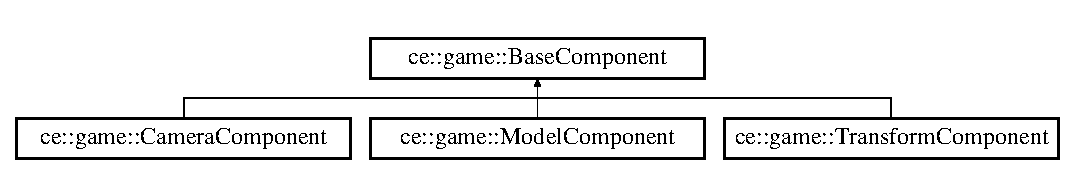
\includegraphics[height=1.904762cm]{classce_1_1game_1_1_base_component}
\end{center}
\end{figure}
\subsection*{Public Member Functions}
\begin{DoxyCompactItemize}
\item 
\mbox{\Hypertarget{classce_1_1game_1_1_base_component_a0b5c620c6b665489b5665621aba17935}\label{classce_1_1game_1_1_base_component_a0b5c620c6b665489b5665621aba17935}} 
virtual void {\bfseries init} ()=0
\item 
\mbox{\Hypertarget{classce_1_1game_1_1_base_component_a0a1cda211f84337d2a33937f89aebd6b}\label{classce_1_1game_1_1_base_component_a0a1cda211f84337d2a33937f89aebd6b}} 
virtual void {\bfseries tick} (float dt)=0
\item 
\mbox{\Hypertarget{classce_1_1game_1_1_base_component_a98da3e6c0af1e20f050ff06749c1299b}\label{classce_1_1game_1_1_base_component_a98da3e6c0af1e20f050ff06749c1299b}} 
virtual void {\bfseries draw} (\hyperlink{classce_1_1graphics_1_1_renderer3_d}{ce\+::graphics\+::\+Renderer3D} $\ast$renderer)=0
\item 
virtual std\+::string \hyperlink{classce_1_1game_1_1_base_component_a1022b55c1926a019a2b3a71fb6b9150e}{get\+Type} ()=0
\begin{DoxyCompactList}\small\item\em Returns the type of Component in a string value. \end{DoxyCompactList}\item 
{\footnotesize template$<$class T $>$ }\\std\+::vector$<$ T $\ast$ $>$ \hyperlink{classce_1_1game_1_1_base_component_af359b12ae4a497e9b36f08286a3849dc}{get\+Host\+Components\+Of\+Type} (std\+::string type)
\end{DoxyCompactItemize}
\subsection*{Public Attributes}
\begin{DoxyCompactItemize}
\item 
\mbox{\Hypertarget{classce_1_1game_1_1_base_component_a5bf4558535c84dc795d7815709cd3e5f}\label{classce_1_1game_1_1_base_component_a5bf4558535c84dc795d7815709cd3e5f}} 
bool {\bfseries b\+Tickable} = false
\item 
\mbox{\Hypertarget{classce_1_1game_1_1_base_component_a3fcb89719c18c4675b2a09c564af86b4}\label{classce_1_1game_1_1_base_component_a3fcb89719c18c4675b2a09c564af86b4}} 
bool {\bfseries b\+Drawable} = false
\end{DoxyCompactItemize}
\subsection*{Protected Attributes}
\begin{DoxyCompactItemize}
\item 
std\+::vector$<$ \hyperlink{classce_1_1game_1_1_base_component}{Base\+Component} $\ast$ $>$ $\ast$ \hyperlink{classce_1_1game_1_1_base_component_ad0448e0b4026fbfee1f88b63ccfbd19c}{m\+\_\+host\+Components}
\begin{DoxyCompactList}\small\item\em Components of this components host(\+Game\+Object) \end{DoxyCompactList}\end{DoxyCompactItemize}
\subsection*{Friends}
\begin{DoxyCompactItemize}
\item 
\mbox{\Hypertarget{classce_1_1game_1_1_base_component_a00df87c957d8f7ee0fc51f07a0542f4a}\label{classce_1_1game_1_1_base_component_a00df87c957d8f7ee0fc51f07a0542f4a}} 
class {\bfseries Game\+Object}
\end{DoxyCompactItemize}


\subsection{Member Function Documentation}
\mbox{\Hypertarget{classce_1_1game_1_1_base_component_af359b12ae4a497e9b36f08286a3849dc}\label{classce_1_1game_1_1_base_component_af359b12ae4a497e9b36f08286a3849dc}} 
\index{ce\+::game\+::\+Base\+Component@{ce\+::game\+::\+Base\+Component}!get\+Host\+Components\+Of\+Type@{get\+Host\+Components\+Of\+Type}}
\index{get\+Host\+Components\+Of\+Type@{get\+Host\+Components\+Of\+Type}!ce\+::game\+::\+Base\+Component@{ce\+::game\+::\+Base\+Component}}
\subsubsection{\texorpdfstring{get\+Host\+Components\+Of\+Type()}{getHostComponentsOfType()}}
{\footnotesize\ttfamily template$<$class T $>$ \\
std\+::vector$<$ T $\ast$ $>$ ce\+::game\+::\+Base\+Component\+::get\+Host\+Components\+Of\+Type (\begin{DoxyParamCaption}\item[{std\+::string}]{type }\end{DoxyParamCaption})\hspace{0.3cm}{\ttfamily [inline]}}

Retrieve all the components of a type from the host

T needs to be the class you are getting as a type as it converts it to that type Returns a vector with the first element being a nullptr if it can\textquotesingle{}t find any \mbox{\Hypertarget{classce_1_1game_1_1_base_component_a1022b55c1926a019a2b3a71fb6b9150e}\label{classce_1_1game_1_1_base_component_a1022b55c1926a019a2b3a71fb6b9150e}} 
\index{ce\+::game\+::\+Base\+Component@{ce\+::game\+::\+Base\+Component}!get\+Type@{get\+Type}}
\index{get\+Type@{get\+Type}!ce\+::game\+::\+Base\+Component@{ce\+::game\+::\+Base\+Component}}
\subsubsection{\texorpdfstring{get\+Type()}{getType()}}
{\footnotesize\ttfamily virtual std\+::string ce\+::game\+::\+Base\+Component\+::get\+Type (\begin{DoxyParamCaption}{ }\end{DoxyParamCaption})\hspace{0.3cm}{\ttfamily [pure virtual]}}



Returns the type of Component in a string value. 

Example\+: Model, Transform etc 

Implemented in \hyperlink{classce_1_1game_1_1_camera_component_a15140bffd017245dd17ed9aa0f953a1b}{ce\+::game\+::\+Camera\+Component}, \hyperlink{classce_1_1game_1_1_model_component_aaac15cad336e35df7be55dda34f53643}{ce\+::game\+::\+Model\+Component}, and \hyperlink{classce_1_1game_1_1_transform_component_ae4a2729b3f88a77b8405de317ab03510}{ce\+::game\+::\+Transform\+Component}.



\subsection{Member Data Documentation}
\mbox{\Hypertarget{classce_1_1game_1_1_base_component_ad0448e0b4026fbfee1f88b63ccfbd19c}\label{classce_1_1game_1_1_base_component_ad0448e0b4026fbfee1f88b63ccfbd19c}} 
\index{ce\+::game\+::\+Base\+Component@{ce\+::game\+::\+Base\+Component}!m\+\_\+host\+Components@{m\+\_\+host\+Components}}
\index{m\+\_\+host\+Components@{m\+\_\+host\+Components}!ce\+::game\+::\+Base\+Component@{ce\+::game\+::\+Base\+Component}}
\subsubsection{\texorpdfstring{m\+\_\+host\+Components}{m\_hostComponents}}
{\footnotesize\ttfamily std\+::vector$<$\hyperlink{classce_1_1game_1_1_base_component}{Base\+Component}$\ast$$>$$\ast$ ce\+::game\+::\+Base\+Component\+::m\+\_\+host\+Components\hspace{0.3cm}{\ttfamily [protected]}}



Components of this components host(\+Game\+Object) 

Used to access other components on the host object such as Transform\+Components etc Since it is a pointer, if the host components change, it is updated here too 

The documentation for this class was generated from the following file\+:\begin{DoxyCompactItemize}
\item 
E\+:/\+Development/\+Game\+Engine/\+C\+Engine/src/\+Game/\+Components/Base\+Component.\+h\end{DoxyCompactItemize}

\hypertarget{classce_1_1graphics_1_1_base_light}{}\section{ce\+:\+:graphics\+:\+:Base\+Light Class Reference}
\label{classce_1_1graphics_1_1_base_light}\index{ce\+::graphics\+::\+Base\+Light@{ce\+::graphics\+::\+Base\+Light}}


Base class for all lights.  




{\ttfamily \#include $<$Lights.\+h$>$}

Inheritance diagram for ce\+:\+:graphics\+:\+:Base\+Light\+:\begin{figure}[H]
\begin{center}
\leavevmode
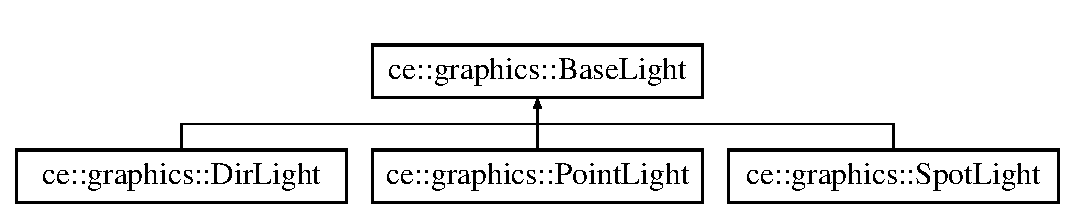
\includegraphics[height=2.000000cm]{classce_1_1graphics_1_1_base_light}
\end{center}
\end{figure}
\subsection*{Public Attributes}
\begin{DoxyCompactItemize}
\item 
\mbox{\Hypertarget{classce_1_1graphics_1_1_base_light_ab7d381028fc562de3e35aaba218e0ef8}\label{classce_1_1graphics_1_1_base_light_ab7d381028fc562de3e35aaba218e0ef8}} 
glm\+::vec3 {\bfseries ambient} = glm\+::vec3(0.\+05f, 0.\+05f, 0.\+05f)
\item 
\mbox{\Hypertarget{classce_1_1graphics_1_1_base_light_a4435de10ee05a5c96bce761b1148d96e}\label{classce_1_1graphics_1_1_base_light_a4435de10ee05a5c96bce761b1148d96e}} 
glm\+::vec3 {\bfseries diffuse} = glm\+::vec3(0.\+5f, 0.\+5f, 0.\+5f)
\item 
\mbox{\Hypertarget{classce_1_1graphics_1_1_base_light_a8aca51622639df6f87b276a9e791f0e5}\label{classce_1_1graphics_1_1_base_light_a8aca51622639df6f87b276a9e791f0e5}} 
glm\+::vec3 {\bfseries specular} = glm\+::vec3(0.\+6f, 0.\+6f, 0.\+6f)
\end{DoxyCompactItemize}


\subsection{Detailed Description}
Base class for all lights. 

The documentation for this class was generated from the following file\+:\begin{DoxyCompactItemize}
\item 
Graphics/\hyperlink{_lights_8h}{Lights.\+h}\end{DoxyCompactItemize}

\hypertarget{classce_1_1game_1_1_camera_component}{}\section{ce\+:\+:game\+:\+:Camera\+Component Class Reference}
\label{classce_1_1game_1_1_camera_component}\index{ce\+::game\+::\+Camera\+Component@{ce\+::game\+::\+Camera\+Component}}
Inheritance diagram for ce\+:\+:game\+:\+:Camera\+Component\+:\begin{figure}[H]
\begin{center}
\leavevmode
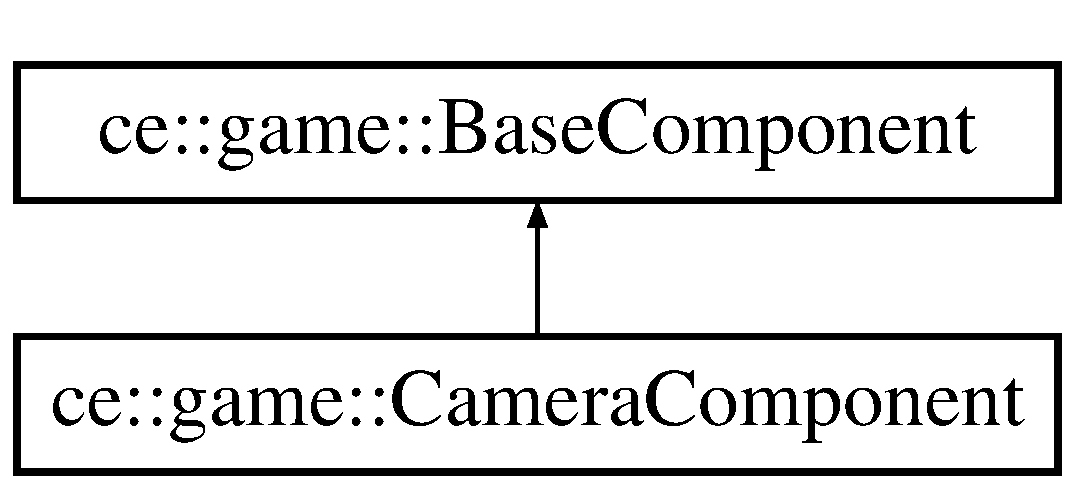
\includegraphics[height=2.000000cm]{classce_1_1game_1_1_camera_component}
\end{center}
\end{figure}
\subsection*{Public Member Functions}
\begin{DoxyCompactItemize}
\item 
\mbox{\Hypertarget{classce_1_1game_1_1_camera_component_a94cd29ec78e415f255691c35482d6870}\label{classce_1_1game_1_1_camera_component_a94cd29ec78e415f255691c35482d6870}} 
virtual void {\bfseries init} () override
\item 
\mbox{\Hypertarget{classce_1_1game_1_1_camera_component_a5657dea10eefa5bc3e9ddb34f5cc34a9}\label{classce_1_1game_1_1_camera_component_a5657dea10eefa5bc3e9ddb34f5cc34a9}} 
virtual void {\bfseries tick} (float dt) override
\item 
\mbox{\Hypertarget{classce_1_1game_1_1_camera_component_ac47d4b1587a57452b611fafe35a3eaf2}\label{classce_1_1game_1_1_camera_component_ac47d4b1587a57452b611fafe35a3eaf2}} 
virtual void {\bfseries draw} (\hyperlink{classce_1_1graphics_1_1_renderer3_d}{ce\+::graphics\+::\+Renderer3D} $\ast$renderer) override
\item 
virtual std\+::string \hyperlink{classce_1_1game_1_1_camera_component_a15140bffd017245dd17ed9aa0f953a1b}{get\+Type} () override
\begin{DoxyCompactList}\small\item\em Returns the type of Component in a string value. \end{DoxyCompactList}\item 
\mbox{\Hypertarget{classce_1_1game_1_1_camera_component_a07df0b85d75a8771727691377c9a4314}\label{classce_1_1game_1_1_camera_component_a07df0b85d75a8771727691377c9a4314}} 
void {\bfseries set\+Projection} (float fov, float aspect\+Ratio, float projnear, float projfar)
\item 
\mbox{\Hypertarget{classce_1_1game_1_1_camera_component_ad439c496f134fcca9a1a232a34603c30}\label{classce_1_1game_1_1_camera_component_ad439c496f134fcca9a1a232a34603c30}} 
glm\+::mat4 {\bfseries get\+Projection\+Matrix} () const
\item 
\mbox{\Hypertarget{classce_1_1game_1_1_camera_component_ac6ef973b5d1b2722257c830fce9e858e}\label{classce_1_1game_1_1_camera_component_ac6ef973b5d1b2722257c830fce9e858e}} 
glm\+::mat4 {\bfseries get\+View\+Matrix} () const
\item 
\mbox{\Hypertarget{classce_1_1game_1_1_camera_component_a1768813779097844b1a55105b19e9509}\label{classce_1_1game_1_1_camera_component_a1768813779097844b1a55105b19e9509}} 
glm\+::vec3 {\bfseries get\+Forward\+Vector} () const
\item 
\mbox{\Hypertarget{classce_1_1game_1_1_camera_component_aa36316887ec2a46098ac554e3e30610a}\label{classce_1_1game_1_1_camera_component_aa36316887ec2a46098ac554e3e30610a}} 
glm\+::vec3 {\bfseries get\+Left\+Vector} () const
\item 
void \hyperlink{classce_1_1game_1_1_camera_component_a8c29ab156769194cc83908467b37beec}{update\+Transform} ()
\begin{DoxyCompactList}\small\item\em Updates the transform component used. \end{DoxyCompactList}\end{DoxyCompactItemize}
\subsection*{Protected Attributes}
\begin{DoxyCompactItemize}
\item 
\mbox{\Hypertarget{classce_1_1game_1_1_camera_component_ab9e91ffab463b69ce6630b81e6cc949d}\label{classce_1_1game_1_1_camera_component_ab9e91ffab463b69ce6630b81e6cc949d}} 
\hyperlink{classce_1_1game_1_1_transform_component}{Transform\+Component} $\ast$ {\bfseries m\+\_\+transform}
\item 
\mbox{\Hypertarget{classce_1_1game_1_1_camera_component_a07d30e0bf458272a54be2e41d06ce73e}\label{classce_1_1game_1_1_camera_component_a07d30e0bf458272a54be2e41d06ce73e}} 
float {\bfseries m\+\_\+fov} = 80.f
\item 
\mbox{\Hypertarget{classce_1_1game_1_1_camera_component_a063122e5cfed1be0ddb7efb3047ce28d}\label{classce_1_1game_1_1_camera_component_a063122e5cfed1be0ddb7efb3047ce28d}} 
float {\bfseries m\+\_\+near} = 0.\+1f
\item 
\mbox{\Hypertarget{classce_1_1game_1_1_camera_component_a4bc867d12c68cfe99b50e75f774de6b9}\label{classce_1_1game_1_1_camera_component_a4bc867d12c68cfe99b50e75f774de6b9}} 
float {\bfseries m\+\_\+far} = 100.f
\item 
\mbox{\Hypertarget{classce_1_1game_1_1_camera_component_aab4b75baa0244460f39d13abae1cbbf5}\label{classce_1_1game_1_1_camera_component_aab4b75baa0244460f39d13abae1cbbf5}} 
float {\bfseries m\+\_\+aspect\+Ratio} = 0.f
\item 
\mbox{\Hypertarget{classce_1_1game_1_1_camera_component_af6c1308a7b8b29f8abf25b7f666037b1}\label{classce_1_1game_1_1_camera_component_af6c1308a7b8b29f8abf25b7f666037b1}} 
glm\+::mat4 {\bfseries m\+\_\+projection}
\end{DoxyCompactItemize}
\subsection*{Additional Inherited Members}


\subsection{Member Function Documentation}
\mbox{\Hypertarget{classce_1_1game_1_1_camera_component_a15140bffd017245dd17ed9aa0f953a1b}\label{classce_1_1game_1_1_camera_component_a15140bffd017245dd17ed9aa0f953a1b}} 
\index{ce\+::game\+::\+Camera\+Component@{ce\+::game\+::\+Camera\+Component}!get\+Type@{get\+Type}}
\index{get\+Type@{get\+Type}!ce\+::game\+::\+Camera\+Component@{ce\+::game\+::\+Camera\+Component}}
\subsubsection{\texorpdfstring{get\+Type()}{getType()}}
{\footnotesize\ttfamily std\+::string ce\+::game\+::\+Camera\+Component\+::get\+Type (\begin{DoxyParamCaption}{ }\end{DoxyParamCaption})\hspace{0.3cm}{\ttfamily [override]}, {\ttfamily [virtual]}}



Returns the type of Component in a string value. 

Example\+: Model, Transform etc 

Implements \hyperlink{classce_1_1game_1_1_base_component_a1022b55c1926a019a2b3a71fb6b9150e}{ce\+::game\+::\+Base\+Component}.

\mbox{\Hypertarget{classce_1_1game_1_1_camera_component_a8c29ab156769194cc83908467b37beec}\label{classce_1_1game_1_1_camera_component_a8c29ab156769194cc83908467b37beec}} 
\index{ce\+::game\+::\+Camera\+Component@{ce\+::game\+::\+Camera\+Component}!update\+Transform@{update\+Transform}}
\index{update\+Transform@{update\+Transform}!ce\+::game\+::\+Camera\+Component@{ce\+::game\+::\+Camera\+Component}}
\subsubsection{\texorpdfstring{update\+Transform()}{updateTransform()}}
{\footnotesize\ttfamily void ce\+::game\+::\+Camera\+Component\+::update\+Transform (\begin{DoxyParamCaption}{ }\end{DoxyParamCaption})}



Updates the transform component used. 

If it cannot find one among it\textquotesingle{}s hosts component list it will set it to a default position 

The documentation for this class was generated from the following files\+:\begin{DoxyCompactItemize}
\item 
E\+:/\+Development/\+Game\+Engine/\+C\+Engine/src/\+Game/\+Components/Camera\+Component.\+h\item 
E\+:/\+Development/\+Game\+Engine/\+C\+Engine/src/\+Game/\+Components/Camera\+Component.\+cpp\end{DoxyCompactItemize}

\hypertarget{structce_1_1graphics_1_1_character}{}\section{ce\+:\+:graphics\+:\+:Character Struct Reference}
\label{structce_1_1graphics_1_1_character}\index{ce\+::graphics\+::\+Character@{ce\+::graphics\+::\+Character}}
\subsection*{Public Attributes}
\begin{DoxyCompactItemize}
\item 
G\+Luint \hyperlink{structce_1_1graphics_1_1_character_ae9dae9443cf985d2e0ee4974ea3a434c}{texture\+ID}
\item 
glm\+::ivec2 \hyperlink{structce_1_1graphics_1_1_character_a6d9408d38c787d6c158db425d2595a02}{size}
\item 
glm\+::ivec2 \hyperlink{structce_1_1graphics_1_1_character_ac4a2c763131a527a79c23607cb3b3218}{bearing}
\item 
G\+Luint \hyperlink{structce_1_1graphics_1_1_character_a9b312a5f9889da34a8406d7193b30961}{advance}
\end{DoxyCompactItemize}


\subsection{Member Data Documentation}
\mbox{\Hypertarget{structce_1_1graphics_1_1_character_a9b312a5f9889da34a8406d7193b30961}\label{structce_1_1graphics_1_1_character_a9b312a5f9889da34a8406d7193b30961}} 
\index{ce\+::graphics\+::\+Character@{ce\+::graphics\+::\+Character}!advance@{advance}}
\index{advance@{advance}!ce\+::graphics\+::\+Character@{ce\+::graphics\+::\+Character}}
\subsubsection{\texorpdfstring{advance}{advance}}
{\footnotesize\ttfamily G\+Luint ce\+::graphics\+::\+Character\+::advance}

Offset to next glyph \mbox{\Hypertarget{structce_1_1graphics_1_1_character_ac4a2c763131a527a79c23607cb3b3218}\label{structce_1_1graphics_1_1_character_ac4a2c763131a527a79c23607cb3b3218}} 
\index{ce\+::graphics\+::\+Character@{ce\+::graphics\+::\+Character}!bearing@{bearing}}
\index{bearing@{bearing}!ce\+::graphics\+::\+Character@{ce\+::graphics\+::\+Character}}
\subsubsection{\texorpdfstring{bearing}{bearing}}
{\footnotesize\ttfamily glm\+::ivec2 ce\+::graphics\+::\+Character\+::bearing}

Offset from baseline to top/left of glyph \mbox{\Hypertarget{structce_1_1graphics_1_1_character_a6d9408d38c787d6c158db425d2595a02}\label{structce_1_1graphics_1_1_character_a6d9408d38c787d6c158db425d2595a02}} 
\index{ce\+::graphics\+::\+Character@{ce\+::graphics\+::\+Character}!size@{size}}
\index{size@{size}!ce\+::graphics\+::\+Character@{ce\+::graphics\+::\+Character}}
\subsubsection{\texorpdfstring{size}{size}}
{\footnotesize\ttfamily glm\+::ivec2 ce\+::graphics\+::\+Character\+::size}

Size of the glyph \mbox{\Hypertarget{structce_1_1graphics_1_1_character_ae9dae9443cf985d2e0ee4974ea3a434c}\label{structce_1_1graphics_1_1_character_ae9dae9443cf985d2e0ee4974ea3a434c}} 
\index{ce\+::graphics\+::\+Character@{ce\+::graphics\+::\+Character}!texture\+ID@{texture\+ID}}
\index{texture\+ID@{texture\+ID}!ce\+::graphics\+::\+Character@{ce\+::graphics\+::\+Character}}
\subsubsection{\texorpdfstring{texture\+ID}{textureID}}
{\footnotesize\ttfamily G\+Luint ce\+::graphics\+::\+Character\+::texture\+ID}

Open\+GL texture id 

The documentation for this struct was generated from the following file\+:\begin{DoxyCompactItemize}
\item 
E\+:/\+Development/\+Game\+Engine/\+C\+Engine/src/\+Graphics/\+Text/Font.\+h\end{DoxyCompactItemize}

\hypertarget{classce_1_1core_1_1_clock}{}\section{ce\+:\+:core\+:\+:Clock Class Reference}
\label{classce_1_1core_1_1_clock}\index{ce\+::core\+::\+Clock@{ce\+::core\+::\+Clock}}


A simple clock.  




{\ttfamily \#include $<$Time.\+h$>$}

\subsection*{Public Member Functions}
\begin{DoxyCompactItemize}
\item 
void \hyperlink{classce_1_1core_1_1_clock_ae8ba6571cfacee77bf76e795969f772a}{start} ()
\item 
\hyperlink{structce_1_1core_1_1_time}{Time} \hyperlink{classce_1_1core_1_1_clock_a9aa3876753067768323f2c260c124a77}{get\+Passed} ()
\item 
\hyperlink{structce_1_1core_1_1_time}{Time} \hyperlink{classce_1_1core_1_1_clock_ad2f5f8ff6d8881ccd8626249232be0f2}{restart} ()
\end{DoxyCompactItemize}


\subsection{Detailed Description}
A simple clock. 

\subsection{Member Function Documentation}
\mbox{\Hypertarget{classce_1_1core_1_1_clock_a9aa3876753067768323f2c260c124a77}\label{classce_1_1core_1_1_clock_a9aa3876753067768323f2c260c124a77}} 
\index{ce\+::core\+::\+Clock@{ce\+::core\+::\+Clock}!get\+Passed@{get\+Passed}}
\index{get\+Passed@{get\+Passed}!ce\+::core\+::\+Clock@{ce\+::core\+::\+Clock}}
\subsubsection{\texorpdfstring{get\+Passed()}{getPassed()}}
{\footnotesize\ttfamily \hyperlink{structce_1_1core_1_1_time}{ce\+::core\+::\+Time} ce\+::core\+::\+Clock\+::get\+Passed (\begin{DoxyParamCaption}{ }\end{DoxyParamCaption})}

Get the \hyperlink{structce_1_1core_1_1_time}{Time} passed since start or restart \mbox{\Hypertarget{classce_1_1core_1_1_clock_ad2f5f8ff6d8881ccd8626249232be0f2}\label{classce_1_1core_1_1_clock_ad2f5f8ff6d8881ccd8626249232be0f2}} 
\index{ce\+::core\+::\+Clock@{ce\+::core\+::\+Clock}!restart@{restart}}
\index{restart@{restart}!ce\+::core\+::\+Clock@{ce\+::core\+::\+Clock}}
\subsubsection{\texorpdfstring{restart()}{restart()}}
{\footnotesize\ttfamily \hyperlink{structce_1_1core_1_1_time}{ce\+::core\+::\+Time} ce\+::core\+::\+Clock\+::restart (\begin{DoxyParamCaption}{ }\end{DoxyParamCaption})}

Get \hyperlink{structce_1_1core_1_1_time}{Time} passed then restart the clock \mbox{\Hypertarget{classce_1_1core_1_1_clock_ae8ba6571cfacee77bf76e795969f772a}\label{classce_1_1core_1_1_clock_ae8ba6571cfacee77bf76e795969f772a}} 
\index{ce\+::core\+::\+Clock@{ce\+::core\+::\+Clock}!start@{start}}
\index{start@{start}!ce\+::core\+::\+Clock@{ce\+::core\+::\+Clock}}
\subsubsection{\texorpdfstring{start()}{start()}}
{\footnotesize\ttfamily void ce\+::core\+::\+Clock\+::start (\begin{DoxyParamCaption}{ }\end{DoxyParamCaption})}

Start clock 

The documentation for this class was generated from the following files\+:\begin{DoxyCompactItemize}
\item 
E\+:/\+Development/\+Game\+Engine/\+C\+Engine/src/\+Core/\hyperlink{_time_8h}{Time.\+h}\item 
E\+:/\+Development/\+Game\+Engine/\+C\+Engine/src/\+Core/Time.\+cpp\end{DoxyCompactItemize}

\hypertarget{classce_1_1graphics_1_1_dir_light}{}\section{ce\+:\+:graphics\+:\+:Dir\+Light Class Reference}
\label{classce_1_1graphics_1_1_dir_light}\index{ce\+::graphics\+::\+Dir\+Light@{ce\+::graphics\+::\+Dir\+Light}}


A directional light.  




{\ttfamily \#include $<$Lights.\+h$>$}

Inheritance diagram for ce\+:\+:graphics\+:\+:Dir\+Light\+:\begin{figure}[H]
\begin{center}
\leavevmode
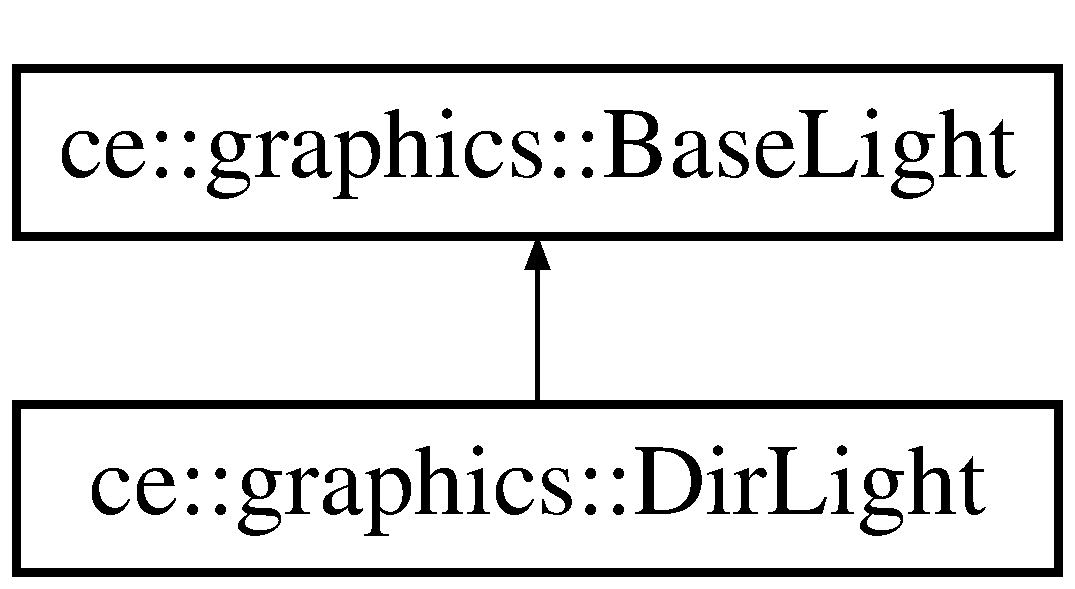
\includegraphics[height=2.000000cm]{classce_1_1graphics_1_1_dir_light}
\end{center}
\end{figure}
\subsection*{Public Attributes}
\begin{DoxyCompactItemize}
\item 
\mbox{\Hypertarget{classce_1_1graphics_1_1_dir_light_a5903f80742e62c8a0fc11499287ca770}\label{classce_1_1graphics_1_1_dir_light_a5903f80742e62c8a0fc11499287ca770}} 
glm\+::vec3 {\bfseries direction} = glm\+::vec3(-\/0.\+5f, -\/0.\+5f, -\/0.\+5f)
\end{DoxyCompactItemize}


\subsection{Detailed Description}
A directional light. 

The documentation for this class was generated from the following file\+:\begin{DoxyCompactItemize}
\item 
E\+:/\+Development/\+Game\+Engine/\+C\+Engine/src/\+Graphics/\hyperlink{_lights_8h}{Lights.\+h}\end{DoxyCompactItemize}

\hypertarget{classce_1_1game_1_1_example_game_mode}{}\section{ce\+:\+:game\+:\+:Example\+Game\+Mode Class Reference}
\label{classce_1_1game_1_1_example_game_mode}\index{ce\+::game\+::\+Example\+Game\+Mode@{ce\+::game\+::\+Example\+Game\+Mode}}
Inheritance diagram for ce\+:\+:game\+:\+:Example\+Game\+Mode\+:\begin{figure}[H]
\begin{center}
\leavevmode
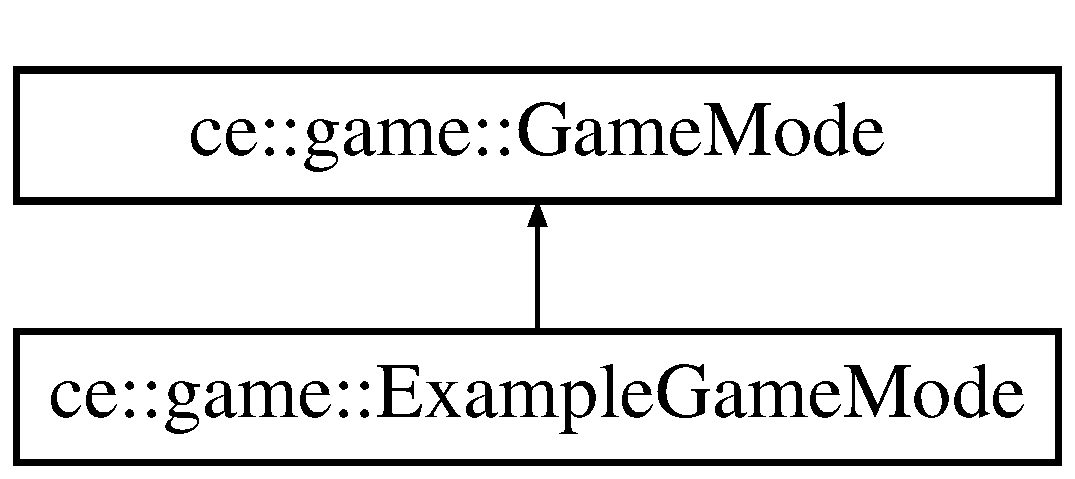
\includegraphics[height=2.000000cm]{classce_1_1game_1_1_example_game_mode}
\end{center}
\end{figure}
\subsection*{Public Member Functions}
\begin{DoxyCompactItemize}
\item 
\mbox{\Hypertarget{classce_1_1game_1_1_example_game_mode_ae08bbb751117cd826545885727fae41b}\label{classce_1_1game_1_1_example_game_mode_ae08bbb751117cd826545885727fae41b}} 
virtual void {\bfseries init} () override
\item 
\mbox{\Hypertarget{classce_1_1game_1_1_example_game_mode_a200d0f3b71ab07bdab9230b105de6bac}\label{classce_1_1game_1_1_example_game_mode_a200d0f3b71ab07bdab9230b105de6bac}} 
virtual void {\bfseries begin} () override
\item 
\mbox{\Hypertarget{classce_1_1game_1_1_example_game_mode_acd316725cc4f51abe7eb61b4be804dac}\label{classce_1_1game_1_1_example_game_mode_acd316725cc4f51abe7eb61b4be804dac}} 
virtual void {\bfseries tick} (float dt) override
\item 
\mbox{\Hypertarget{classce_1_1game_1_1_example_game_mode_a17988b5f1abacb284409f3826c9ce64c}\label{classce_1_1game_1_1_example_game_mode_a17988b5f1abacb284409f3826c9ce64c}} 
virtual void {\bfseries draw} () override
\item 
\mbox{\Hypertarget{classce_1_1game_1_1_example_game_mode_ae7815142c00b85327835141a24628663}\label{classce_1_1game_1_1_example_game_mode_ae7815142c00b85327835141a24628663}} 
virtual void {\bfseries end} () override
\item 
\mbox{\Hypertarget{classce_1_1game_1_1_example_game_mode_a91b064233b7c03e6c0c63bf51c105784}\label{classce_1_1game_1_1_example_game_mode_a91b064233b7c03e6c0c63bf51c105784}} 
void {\bfseries camera\+Yaw} (float axis)
\item 
\mbox{\Hypertarget{classce_1_1game_1_1_example_game_mode_af6c617e23e9d1aec177bff7acc8e7580}\label{classce_1_1game_1_1_example_game_mode_af6c617e23e9d1aec177bff7acc8e7580}} 
void {\bfseries camera\+Pitch} (float axis)
\item 
\mbox{\Hypertarget{classce_1_1game_1_1_example_game_mode_aa182d698fd87627ea26f4491624d02ed}\label{classce_1_1game_1_1_example_game_mode_aa182d698fd87627ea26f4491624d02ed}} 
void {\bfseries move\+Left} (bool pressed)
\item 
\mbox{\Hypertarget{classce_1_1game_1_1_example_game_mode_a1cf327605a6ac3e6607c5eb92e3c781a}\label{classce_1_1game_1_1_example_game_mode_a1cf327605a6ac3e6607c5eb92e3c781a}} 
void {\bfseries move\+Right} (bool pressed)
\item 
\mbox{\Hypertarget{classce_1_1game_1_1_example_game_mode_a082495a05e87ea2033a285a5b5a342ec}\label{classce_1_1game_1_1_example_game_mode_a082495a05e87ea2033a285a5b5a342ec}} 
void {\bfseries move\+Forward} (bool pressed)
\item 
\mbox{\Hypertarget{classce_1_1game_1_1_example_game_mode_a72df4703c38309dfa8366689783746a0}\label{classce_1_1game_1_1_example_game_mode_a72df4703c38309dfa8366689783746a0}} 
void {\bfseries move\+Backward} (bool pressed)
\item 
\mbox{\Hypertarget{classce_1_1game_1_1_example_game_mode_a958ce18d291b1d1b3628172607f44a55}\label{classce_1_1game_1_1_example_game_mode_a958ce18d291b1d1b3628172607f44a55}} 
void {\bfseries move\+P\+LightF} (bool pressed)
\item 
\mbox{\Hypertarget{classce_1_1game_1_1_example_game_mode_a3f7ade0b7e5de15e33e119840b75eca1}\label{classce_1_1game_1_1_example_game_mode_a3f7ade0b7e5de15e33e119840b75eca1}} 
void {\bfseries move\+P\+LightB} (bool pressed)
\item 
\mbox{\Hypertarget{classce_1_1game_1_1_example_game_mode_a11fb49eb30231a59851ab5262b2471cd}\label{classce_1_1game_1_1_example_game_mode_a11fb49eb30231a59851ab5262b2471cd}} 
void {\bfseries move\+P\+LightL} (bool pressed)
\item 
\mbox{\Hypertarget{classce_1_1game_1_1_example_game_mode_a660e5d4bcf5a0188d3ae7f15d2f144e4}\label{classce_1_1game_1_1_example_game_mode_a660e5d4bcf5a0188d3ae7f15d2f144e4}} 
void {\bfseries move\+P\+LightR} (bool pressed)
\end{DoxyCompactItemize}
\subsection*{Protected Attributes}
\begin{DoxyCompactItemize}
\item 
\mbox{\Hypertarget{classce_1_1game_1_1_example_game_mode_a7a086bf963cd0f90bce90f7bf408f718}\label{classce_1_1game_1_1_example_game_mode_a7a086bf963cd0f90bce90f7bf408f718}} 
\hyperlink{classce_1_1game_1_1_transform_component}{ce\+::game\+::\+Transform\+Component} {\bfseries m\+\_\+transform\+Component}
\item 
\mbox{\Hypertarget{classce_1_1game_1_1_example_game_mode_a4d3e7de3f088f8e0cbb3933bf4b51eb9}\label{classce_1_1game_1_1_example_game_mode_a4d3e7de3f088f8e0cbb3933bf4b51eb9}} 
\hyperlink{classce_1_1game_1_1_model_component}{ce\+::game\+::\+Model\+Component} {\bfseries m\+\_\+model\+Component}
\item 
\mbox{\Hypertarget{classce_1_1game_1_1_example_game_mode_afeb8258af62acab90107035f2bbbb074}\label{classce_1_1game_1_1_example_game_mode_afeb8258af62acab90107035f2bbbb074}} 
\hyperlink{classce_1_1game_1_1_transform_component}{ce\+::game\+::\+Transform\+Component} {\bfseries m\+\_\+transform\+Component\+Grassy}
\item 
\mbox{\Hypertarget{classce_1_1game_1_1_example_game_mode_a61458c1f82c751975d11714b3a20a3b8}\label{classce_1_1game_1_1_example_game_mode_a61458c1f82c751975d11714b3a20a3b8}} 
\hyperlink{classce_1_1game_1_1_model_component}{ce\+::game\+::\+Model\+Component} {\bfseries m\+\_\+model\+Component\+Grassy}
\item 
\mbox{\Hypertarget{classce_1_1game_1_1_example_game_mode_a56415cf24321a3f414242f541a97843e}\label{classce_1_1game_1_1_example_game_mode_a56415cf24321a3f414242f541a97843e}} 
\hyperlink{classce_1_1game_1_1_transform_component}{ce\+::game\+::\+Transform\+Component} {\bfseries m\+\_\+camera\+Transform}
\item 
\mbox{\Hypertarget{classce_1_1game_1_1_example_game_mode_a78332e850a9f6a7f7309b3226d42bd41}\label{classce_1_1game_1_1_example_game_mode_a78332e850a9f6a7f7309b3226d42bd41}} 
\hyperlink{classce_1_1game_1_1_camera_component}{ce\+::game\+::\+Camera\+Component} {\bfseries m\+\_\+camera}
\item 
\mbox{\Hypertarget{classce_1_1game_1_1_example_game_mode_a533941188b8d130f9ae2c91c157b18c9}\label{classce_1_1game_1_1_example_game_mode_a533941188b8d130f9ae2c91c157b18c9}} 
\hyperlink{classce_1_1graphics_1_1_forward_renderer}{ce\+::graphics\+::\+Forward\+Renderer} {\bfseries m\+\_\+renderer}
\item 
\mbox{\Hypertarget{classce_1_1game_1_1_example_game_mode_ab39f4d293ea643da5ccac64011366209}\label{classce_1_1game_1_1_example_game_mode_ab39f4d293ea643da5ccac64011366209}} 
\hyperlink{structce_1_1graphics_1_1_light_setup}{ce\+::graphics\+::\+Light\+Setup} {\bfseries m\+\_\+lights}
\item 
\mbox{\Hypertarget{classce_1_1game_1_1_example_game_mode_aba71b1c261ba5df986a23915413f31e0}\label{classce_1_1game_1_1_example_game_mode_aba71b1c261ba5df986a23915413f31e0}} 
bool {\bfseries m\+\_\+move\+Forward} = false
\item 
\mbox{\Hypertarget{classce_1_1game_1_1_example_game_mode_aacf6c7d0c299cbf0ca24e1e952c3f24a}\label{classce_1_1game_1_1_example_game_mode_aacf6c7d0c299cbf0ca24e1e952c3f24a}} 
bool {\bfseries m\+\_\+move\+Backward} = false
\item 
\mbox{\Hypertarget{classce_1_1game_1_1_example_game_mode_a95c5e1b487e7dda6ac2214a9a3b8c058}\label{classce_1_1game_1_1_example_game_mode_a95c5e1b487e7dda6ac2214a9a3b8c058}} 
bool {\bfseries m\+\_\+move\+Left} = false
\item 
\mbox{\Hypertarget{classce_1_1game_1_1_example_game_mode_aa45b83aacdc3f4077bd7acb6a55df3f7}\label{classce_1_1game_1_1_example_game_mode_aa45b83aacdc3f4077bd7acb6a55df3f7}} 
bool {\bfseries m\+\_\+move\+Right} = false
\item 
\mbox{\Hypertarget{classce_1_1game_1_1_example_game_mode_afe9771c52e97b45cc7e509c390c797a3}\label{classce_1_1game_1_1_example_game_mode_afe9771c52e97b45cc7e509c390c797a3}} 
float {\bfseries m\+\_\+orient\+Yaw} = 0.\+0f
\item 
\mbox{\Hypertarget{classce_1_1game_1_1_example_game_mode_ae0e5978dfa5f3cd1dc3bde8c6d44effb}\label{classce_1_1game_1_1_example_game_mode_ae0e5978dfa5f3cd1dc3bde8c6d44effb}} 
float {\bfseries m\+\_\+orient\+Pitch} = 0.\+0f
\end{DoxyCompactItemize}


The documentation for this class was generated from the following files\+:\begin{DoxyCompactItemize}
\item 
E\+:/\+Development/\+Game\+Engine/\+C\+Engine/src/\+Game/\+Game\+Mode/Example\+Game\+Mode.\+h\item 
E\+:/\+Development/\+Game\+Engine/\+C\+Engine/src/\+Game/\+Game\+Mode/Example\+Game\+Mode.\+cpp\end{DoxyCompactItemize}

\hypertarget{classce_1_1graphics_1_1_font}{}\section{ce\+:\+:graphics\+:\+:Font Class Reference}
\label{classce_1_1graphics_1_1_font}\index{ce\+::graphics\+::\+Font@{ce\+::graphics\+::\+Font}}
\subsection*{Public Member Functions}
\begin{DoxyCompactItemize}
\item 
\mbox{\Hypertarget{classce_1_1graphics_1_1_font_ae6c746d596ba69ab989bf083aea235a8}\label{classce_1_1graphics_1_1_font_ae6c746d596ba69ab989bf083aea235a8}} 
{\bfseries Font} (std\+::string path)
\item 
\mbox{\Hypertarget{classce_1_1graphics_1_1_font_ab8fce3029f631939c54c9a6e05864e1f}\label{classce_1_1graphics_1_1_font_ab8fce3029f631939c54c9a6e05864e1f}} 
bool {\bfseries load} (std\+::string path)
\item 
\hyperlink{structce_1_1graphics_1_1_character}{Character} \hyperlink{classce_1_1graphics_1_1_font_a44ef17f6322eae8cd5fa1d2ceea86ad1}{get\+Character} (unsigned long char\+Code, unsigned int height=48, unsigned int width=0)
\begin{DoxyCompactList}\small\item\em Retrieve a character from the font. \end{DoxyCompactList}\end{DoxyCompactItemize}
\subsection*{Protected Attributes}
\begin{DoxyCompactItemize}
\item 
\mbox{\Hypertarget{classce_1_1graphics_1_1_font_a74867445b0dabfed45454e5706bae25c}\label{classce_1_1graphics_1_1_font_a74867445b0dabfed45454e5706bae25c}} 
F\+T\+\_\+\+Face {\bfseries m\+\_\+ft\+Face}
\end{DoxyCompactItemize}


\subsection{Member Function Documentation}
\mbox{\Hypertarget{classce_1_1graphics_1_1_font_a44ef17f6322eae8cd5fa1d2ceea86ad1}\label{classce_1_1graphics_1_1_font_a44ef17f6322eae8cd5fa1d2ceea86ad1}} 
\index{ce\+::graphics\+::\+Font@{ce\+::graphics\+::\+Font}!get\+Character@{get\+Character}}
\index{get\+Character@{get\+Character}!ce\+::graphics\+::\+Font@{ce\+::graphics\+::\+Font}}
\subsubsection{\texorpdfstring{get\+Character()}{getCharacter()}}
{\footnotesize\ttfamily \hyperlink{structce_1_1graphics_1_1_character}{ce\+::graphics\+::\+Character} ce\+::graphics\+::\+Font\+::get\+Character (\begin{DoxyParamCaption}\item[{unsigned long}]{char\+Code,  }\item[{unsigned int}]{height = {\ttfamily 48},  }\item[{unsigned int}]{width = {\ttfamily 0} }\end{DoxyParamCaption})}



Retrieve a character from the font. 


\begin{DoxyParams}{Parameters}
{\em char\+Code} & the code of the character we wish to retrieve \\
\hline
{\em height} & the height of the character \\
\hline
{\em width} & the width of the character, 0 for dynamic \\
\hline
\end{DoxyParams}


The documentation for this class was generated from the following files\+:\begin{DoxyCompactItemize}
\item 
E\+:/\+Development/\+Game\+Engine/\+C\+Engine/src/\+Graphics/\+Text/Font.\+h\item 
E\+:/\+Development/\+Game\+Engine/\+C\+Engine/src/\+Graphics/\+Text/Font.\+cpp\end{DoxyCompactItemize}

\hypertarget{classce_1_1graphics_1_1_forward_renderer}{}\section{ce\+:\+:graphics\+:\+:Forward\+Renderer Class Reference}
\label{classce_1_1graphics_1_1_forward_renderer}\index{ce\+::graphics\+::\+Forward\+Renderer@{ce\+::graphics\+::\+Forward\+Renderer}}
Inheritance diagram for ce\+:\+:graphics\+:\+:Forward\+Renderer\+:\begin{figure}[H]
\begin{center}
\leavevmode
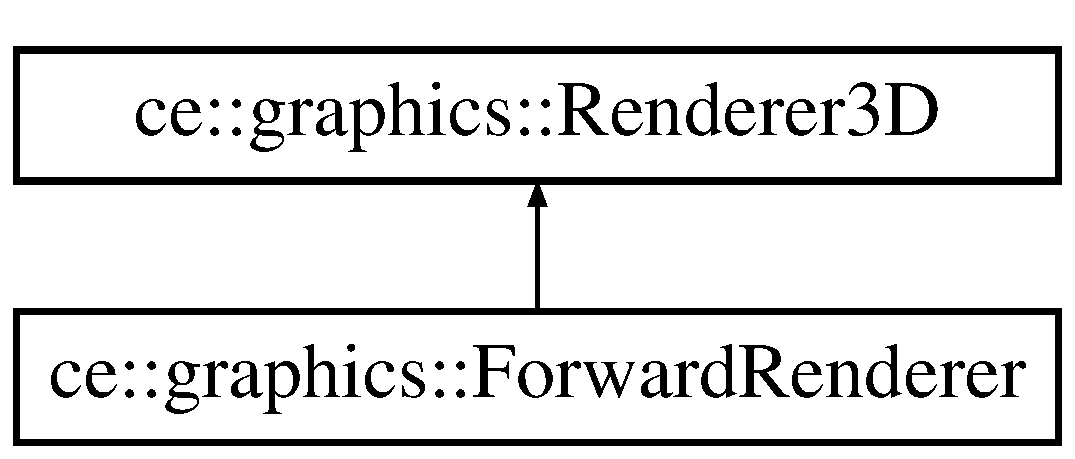
\includegraphics[height=2.000000cm]{classce_1_1graphics_1_1_forward_renderer}
\end{center}
\end{figure}
\subsection*{Public Member Functions}
\begin{DoxyCompactItemize}
\item 
void \hyperlink{classce_1_1graphics_1_1_forward_renderer_ac6c7ad9a18ecfb2cbb6aee202e7e2e8f}{init} () override
\item 
void \hyperlink{classce_1_1graphics_1_1_forward_renderer_a4550120dc1349b5298de4a02422c6c26}{begin} () override
\item 
void \hyperlink{classce_1_1graphics_1_1_forward_renderer_ae84dbf0b5a71b464cf4fc34a5daac805}{begin\+Scene} (\hyperlink{classce_1_1graphics_1_1_camera}{Camera} $\ast$camera) override
\item 
void \hyperlink{classce_1_1graphics_1_1_forward_renderer_a3fb15f85368a78834b9d25b98461916c}{submit} (const \hyperlink{structce_1_1graphics_1_1_render_command}{Render\+Command} \&command) override
\item 
void \hyperlink{classce_1_1graphics_1_1_forward_renderer_abfb5f86e8b5c6a1824ab7a03838785fd}{submit\+Mesh} (\hyperlink{classce_1_1graphics_1_1_mesh}{Mesh} $\ast$mesh, const glm\+::mat4 \&transform) override
\item 
void \hyperlink{classce_1_1graphics_1_1_forward_renderer_a32c92d13c2ba951f71552ea9cf15350c}{submit\+Light\+Setup} (const \hyperlink{structce_1_1graphics_1_1_light_setup}{Light\+Setup} \&light\+Setup) override
\item 
void \hyperlink{classce_1_1graphics_1_1_forward_renderer_a34bf60e44a9a594ab596f46ca7688e3e}{end\+Scene} () override
\item 
void \hyperlink{classce_1_1graphics_1_1_forward_renderer_a8a8c16a645e63fd54b932f62d96d805b}{end} () override
\item 
void \hyperlink{classce_1_1graphics_1_1_forward_renderer_a19933a9015f2abbd27b398e7a6d697b6}{present} () override
\end{DoxyCompactItemize}
\subsection*{Additional Inherited Members}


\subsection{Member Function Documentation}
\mbox{\Hypertarget{classce_1_1graphics_1_1_forward_renderer_a4550120dc1349b5298de4a02422c6c26}\label{classce_1_1graphics_1_1_forward_renderer_a4550120dc1349b5298de4a02422c6c26}} 
\index{ce\+::graphics\+::\+Forward\+Renderer@{ce\+::graphics\+::\+Forward\+Renderer}!begin@{begin}}
\index{begin@{begin}!ce\+::graphics\+::\+Forward\+Renderer@{ce\+::graphics\+::\+Forward\+Renderer}}
\subsubsection{\texorpdfstring{begin()}{begin()}}
{\footnotesize\ttfamily void ce\+::graphics\+::\+Forward\+Renderer\+::begin (\begin{DoxyParamCaption}{ }\end{DoxyParamCaption})\hspace{0.3cm}{\ttfamily [override]}, {\ttfamily [virtual]}}

Begining stage of the renderer 

Implements \hyperlink{classce_1_1graphics_1_1_renderer3_d_a51818b5b581c33001ddbbc6dff9d6e36}{ce\+::graphics\+::\+Renderer3D}.

\mbox{\Hypertarget{classce_1_1graphics_1_1_forward_renderer_ae84dbf0b5a71b464cf4fc34a5daac805}\label{classce_1_1graphics_1_1_forward_renderer_ae84dbf0b5a71b464cf4fc34a5daac805}} 
\index{ce\+::graphics\+::\+Forward\+Renderer@{ce\+::graphics\+::\+Forward\+Renderer}!begin\+Scene@{begin\+Scene}}
\index{begin\+Scene@{begin\+Scene}!ce\+::graphics\+::\+Forward\+Renderer@{ce\+::graphics\+::\+Forward\+Renderer}}
\subsubsection{\texorpdfstring{begin\+Scene()}{beginScene()}}
{\footnotesize\ttfamily void ce\+::graphics\+::\+Forward\+Renderer\+::begin\+Scene (\begin{DoxyParamCaption}\item[{\hyperlink{classce_1_1graphics_1_1_camera}{Camera} $\ast$}]{camera }\end{DoxyParamCaption})\hspace{0.3cm}{\ttfamily [override]}, {\ttfamily [virtual]}}

Begining of the scene 

Implements \hyperlink{classce_1_1graphics_1_1_renderer3_d_a94e60931e0ff3f26b217db09a11ee7e6}{ce\+::graphics\+::\+Renderer3D}.

\mbox{\Hypertarget{classce_1_1graphics_1_1_forward_renderer_a8a8c16a645e63fd54b932f62d96d805b}\label{classce_1_1graphics_1_1_forward_renderer_a8a8c16a645e63fd54b932f62d96d805b}} 
\index{ce\+::graphics\+::\+Forward\+Renderer@{ce\+::graphics\+::\+Forward\+Renderer}!end@{end}}
\index{end@{end}!ce\+::graphics\+::\+Forward\+Renderer@{ce\+::graphics\+::\+Forward\+Renderer}}
\subsubsection{\texorpdfstring{end()}{end()}}
{\footnotesize\ttfamily void ce\+::graphics\+::\+Forward\+Renderer\+::end (\begin{DoxyParamCaption}{ }\end{DoxyParamCaption})\hspace{0.3cm}{\ttfamily [override]}, {\ttfamily [virtual]}}

Render loop ending 

Implements \hyperlink{classce_1_1graphics_1_1_renderer3_d_a4d35e07f42a4fb42ebe3f8e57bfcdb58}{ce\+::graphics\+::\+Renderer3D}.

\mbox{\Hypertarget{classce_1_1graphics_1_1_forward_renderer_a34bf60e44a9a594ab596f46ca7688e3e}\label{classce_1_1graphics_1_1_forward_renderer_a34bf60e44a9a594ab596f46ca7688e3e}} 
\index{ce\+::graphics\+::\+Forward\+Renderer@{ce\+::graphics\+::\+Forward\+Renderer}!end\+Scene@{end\+Scene}}
\index{end\+Scene@{end\+Scene}!ce\+::graphics\+::\+Forward\+Renderer@{ce\+::graphics\+::\+Forward\+Renderer}}
\subsubsection{\texorpdfstring{end\+Scene()}{endScene()}}
{\footnotesize\ttfamily void ce\+::graphics\+::\+Forward\+Renderer\+::end\+Scene (\begin{DoxyParamCaption}{ }\end{DoxyParamCaption})\hspace{0.3cm}{\ttfamily [override]}, {\ttfamily [virtual]}}

Scene ending 

Implements \hyperlink{classce_1_1graphics_1_1_renderer3_d_a0b8feaf1dd7f6ee03c7be2197d012e25}{ce\+::graphics\+::\+Renderer3D}.

\mbox{\Hypertarget{classce_1_1graphics_1_1_forward_renderer_ac6c7ad9a18ecfb2cbb6aee202e7e2e8f}\label{classce_1_1graphics_1_1_forward_renderer_ac6c7ad9a18ecfb2cbb6aee202e7e2e8f}} 
\index{ce\+::graphics\+::\+Forward\+Renderer@{ce\+::graphics\+::\+Forward\+Renderer}!init@{init}}
\index{init@{init}!ce\+::graphics\+::\+Forward\+Renderer@{ce\+::graphics\+::\+Forward\+Renderer}}
\subsubsection{\texorpdfstring{init()}{init()}}
{\footnotesize\ttfamily void ce\+::graphics\+::\+Forward\+Renderer\+::init (\begin{DoxyParamCaption}{ }\end{DoxyParamCaption})\hspace{0.3cm}{\ttfamily [override]}, {\ttfamily [virtual]}}

Initialization stage of the renderer 

Implements \hyperlink{classce_1_1graphics_1_1_renderer3_d_ae887bbdc74af40838e6d059d30bb430b}{ce\+::graphics\+::\+Renderer3D}.

\mbox{\Hypertarget{classce_1_1graphics_1_1_forward_renderer_a19933a9015f2abbd27b398e7a6d697b6}\label{classce_1_1graphics_1_1_forward_renderer_a19933a9015f2abbd27b398e7a6d697b6}} 
\index{ce\+::graphics\+::\+Forward\+Renderer@{ce\+::graphics\+::\+Forward\+Renderer}!present@{present}}
\index{present@{present}!ce\+::graphics\+::\+Forward\+Renderer@{ce\+::graphics\+::\+Forward\+Renderer}}
\subsubsection{\texorpdfstring{present()}{present()}}
{\footnotesize\ttfamily void ce\+::graphics\+::\+Forward\+Renderer\+::present (\begin{DoxyParamCaption}{ }\end{DoxyParamCaption})\hspace{0.3cm}{\ttfamily [override]}, {\ttfamily [virtual]}}

Do the actual rendering and present it on screen 

Implements \hyperlink{classce_1_1graphics_1_1_renderer3_d_a7b258350b5af957550a2d29800d3c5b7}{ce\+::graphics\+::\+Renderer3D}.

\mbox{\Hypertarget{classce_1_1graphics_1_1_forward_renderer_a3fb15f85368a78834b9d25b98461916c}\label{classce_1_1graphics_1_1_forward_renderer_a3fb15f85368a78834b9d25b98461916c}} 
\index{ce\+::graphics\+::\+Forward\+Renderer@{ce\+::graphics\+::\+Forward\+Renderer}!submit@{submit}}
\index{submit@{submit}!ce\+::graphics\+::\+Forward\+Renderer@{ce\+::graphics\+::\+Forward\+Renderer}}
\subsubsection{\texorpdfstring{submit()}{submit()}}
{\footnotesize\ttfamily void ce\+::graphics\+::\+Forward\+Renderer\+::submit (\begin{DoxyParamCaption}\item[{const \hyperlink{structce_1_1graphics_1_1_render_command}{Render\+Command} \&}]{command }\end{DoxyParamCaption})\hspace{0.3cm}{\ttfamily [override]}, {\ttfamily [virtual]}}

Submit a render command 

Implements \hyperlink{classce_1_1graphics_1_1_renderer3_d_a67e956930a17600cdcfc689aa624f990}{ce\+::graphics\+::\+Renderer3D}.

\mbox{\Hypertarget{classce_1_1graphics_1_1_forward_renderer_a32c92d13c2ba951f71552ea9cf15350c}\label{classce_1_1graphics_1_1_forward_renderer_a32c92d13c2ba951f71552ea9cf15350c}} 
\index{ce\+::graphics\+::\+Forward\+Renderer@{ce\+::graphics\+::\+Forward\+Renderer}!submit\+Light\+Setup@{submit\+Light\+Setup}}
\index{submit\+Light\+Setup@{submit\+Light\+Setup}!ce\+::graphics\+::\+Forward\+Renderer@{ce\+::graphics\+::\+Forward\+Renderer}}
\subsubsection{\texorpdfstring{submit\+Light\+Setup()}{submitLightSetup()}}
{\footnotesize\ttfamily void ce\+::graphics\+::\+Forward\+Renderer\+::submit\+Light\+Setup (\begin{DoxyParamCaption}\item[{const \hyperlink{structce_1_1graphics_1_1_light_setup}{Light\+Setup} \&}]{light\+Setup }\end{DoxyParamCaption})\hspace{0.3cm}{\ttfamily [override]}, {\ttfamily [virtual]}}

Submit the light setup to use 

Implements \hyperlink{classce_1_1graphics_1_1_renderer3_d_a4a2eb6efe3adbff611c20141159eb3dc}{ce\+::graphics\+::\+Renderer3D}.

\mbox{\Hypertarget{classce_1_1graphics_1_1_forward_renderer_abfb5f86e8b5c6a1824ab7a03838785fd}\label{classce_1_1graphics_1_1_forward_renderer_abfb5f86e8b5c6a1824ab7a03838785fd}} 
\index{ce\+::graphics\+::\+Forward\+Renderer@{ce\+::graphics\+::\+Forward\+Renderer}!submit\+Mesh@{submit\+Mesh}}
\index{submit\+Mesh@{submit\+Mesh}!ce\+::graphics\+::\+Forward\+Renderer@{ce\+::graphics\+::\+Forward\+Renderer}}
\subsubsection{\texorpdfstring{submit\+Mesh()}{submitMesh()}}
{\footnotesize\ttfamily void ce\+::graphics\+::\+Forward\+Renderer\+::submit\+Mesh (\begin{DoxyParamCaption}\item[{\hyperlink{classce_1_1graphics_1_1_mesh}{Mesh} $\ast$}]{mesh,  }\item[{const glm\+::mat4 \&}]{transform }\end{DoxyParamCaption})\hspace{0.3cm}{\ttfamily [override]}, {\ttfamily [virtual]}}

Submit a lone mesh 

Implements \hyperlink{classce_1_1graphics_1_1_renderer3_d_aba7b0abfa0aad0d89a816923e83ef787}{ce\+::graphics\+::\+Renderer3D}.



The documentation for this class was generated from the following files\+:\begin{DoxyCompactItemize}
\item 
E\+:/\+Development/\+Game\+Engine/\+C\+Engine/src/\+Graphics/\+Renderer/\hyperlink{_forward_renderer_8h}{Forward\+Renderer.\+h}\item 
E\+:/\+Development/\+Game\+Engine/\+C\+Engine/src/\+Graphics/\+Renderer/Forward\+Renderer.\+cpp\end{DoxyCompactItemize}

\hypertarget{classce_1_1game_1_1_game_mode}{}\section{ce\+:\+:game\+:\+:Game\+Mode Class Reference}
\label{classce_1_1game_1_1_game_mode}\index{ce\+::game\+::\+Game\+Mode@{ce\+::game\+::\+Game\+Mode}}
Inheritance diagram for ce\+:\+:game\+:\+:Game\+Mode\+:\begin{figure}[H]
\begin{center}
\leavevmode
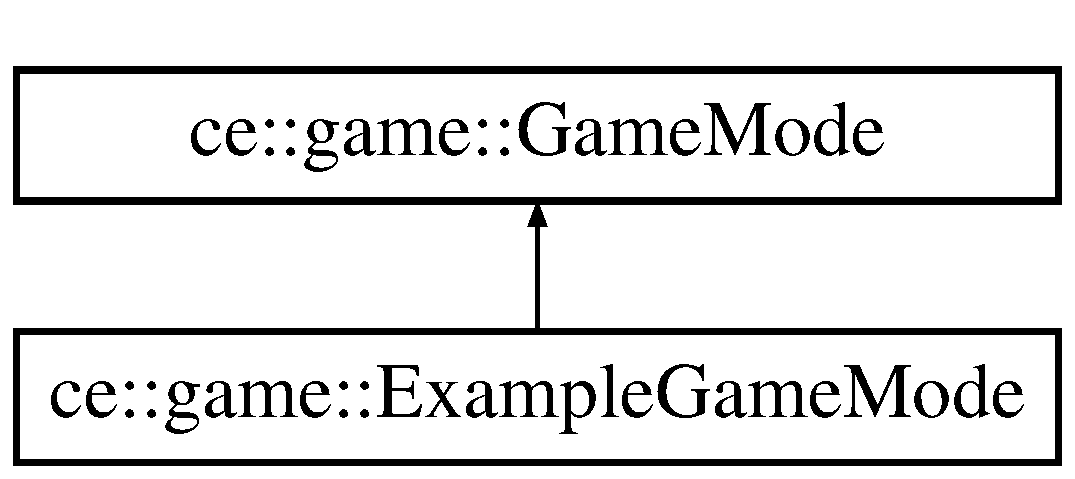
\includegraphics[height=2.000000cm]{classce_1_1game_1_1_game_mode}
\end{center}
\end{figure}
\subsection*{Public Member Functions}
\begin{DoxyCompactItemize}
\item 
\mbox{\Hypertarget{classce_1_1game_1_1_game_mode_a69e86b5a58df6b151ddb6916edf30715}\label{classce_1_1game_1_1_game_mode_a69e86b5a58df6b151ddb6916edf30715}} 
void {\bfseries check\+Input} (const S\+D\+L\+\_\+\+Event \&input)
\item 
\mbox{\Hypertarget{classce_1_1game_1_1_game_mode_a43931c8e739b445b13cc024aaf003ba0}\label{classce_1_1game_1_1_game_mode_a43931c8e739b445b13cc024aaf003ba0}} 
virtual void {\bfseries init} ()
\item 
\mbox{\Hypertarget{classce_1_1game_1_1_game_mode_a39d9f02347519e8abad23fde6884edf5}\label{classce_1_1game_1_1_game_mode_a39d9f02347519e8abad23fde6884edf5}} 
virtual void {\bfseries begin} ()
\item 
\mbox{\Hypertarget{classce_1_1game_1_1_game_mode_af67c1ea425459b53db1d0abd0f549090}\label{classce_1_1game_1_1_game_mode_af67c1ea425459b53db1d0abd0f549090}} 
virtual void {\bfseries tick} (float dt)
\item 
\mbox{\Hypertarget{classce_1_1game_1_1_game_mode_a5ccf2272ba8548386429b52f7a090eb0}\label{classce_1_1game_1_1_game_mode_a5ccf2272ba8548386429b52f7a090eb0}} 
virtual void {\bfseries draw} ()=0
\item 
\mbox{\Hypertarget{classce_1_1game_1_1_game_mode_a332548788e31a178c64877e5cc8c0cda}\label{classce_1_1game_1_1_game_mode_a332548788e31a178c64877e5cc8c0cda}} 
virtual void {\bfseries end} ()
\item 
\mbox{\Hypertarget{classce_1_1game_1_1_game_mode_a82f96a29888897674176e628cd2a7c0d}\label{classce_1_1game_1_1_game_mode_a82f96a29888897674176e628cd2a7c0d}} 
void {\bfseries draw} (\hyperlink{classce_1_1graphics_1_1_renderer3_d}{ce\+::graphics\+::\+Renderer3D} $\ast$renderer)
\end{DoxyCompactItemize}
\subsection*{Protected Attributes}
\begin{DoxyCompactItemize}
\item 
\mbox{\Hypertarget{classce_1_1game_1_1_game_mode_afe021159648ad025aa1657a5096617c0}\label{classce_1_1game_1_1_game_mode_afe021159648ad025aa1657a5096617c0}} 
\hyperlink{classce_1_1game_1_1_scene}{ce\+::game\+::\+Scene} {\bfseries m\+\_\+scene}
\item 
\mbox{\Hypertarget{classce_1_1game_1_1_game_mode_a784f9c9163634f8c76858f3eb19f4f11}\label{classce_1_1game_1_1_game_mode_a784f9c9163634f8c76858f3eb19f4f11}} 
\hyperlink{classce_1_1core_1_1_input}{ce\+::core\+::\+Input} {\bfseries m\+\_\+input}
\end{DoxyCompactItemize}


The documentation for this class was generated from the following files\+:\begin{DoxyCompactItemize}
\item 
E\+:/\+Development/\+Game\+Engine/\+C\+Engine/src/\+Game/\+Game\+Mode/Game\+Mode.\+h\item 
E\+:/\+Development/\+Game\+Engine/\+C\+Engine/src/\+Game/\+Game\+Mode/Game\+Mode.\+cpp\end{DoxyCompactItemize}

\hypertarget{classce_1_1game_1_1_game_object}{}\section{ce\+:\+:game\+:\+:Game\+Object Class Reference}
\label{classce_1_1game_1_1_game_object}\index{ce\+::game\+::\+Game\+Object@{ce\+::game\+::\+Game\+Object}}
Inheritance diagram for ce\+:\+:game\+:\+:Game\+Object\+:\begin{figure}[H]
\begin{center}
\leavevmode
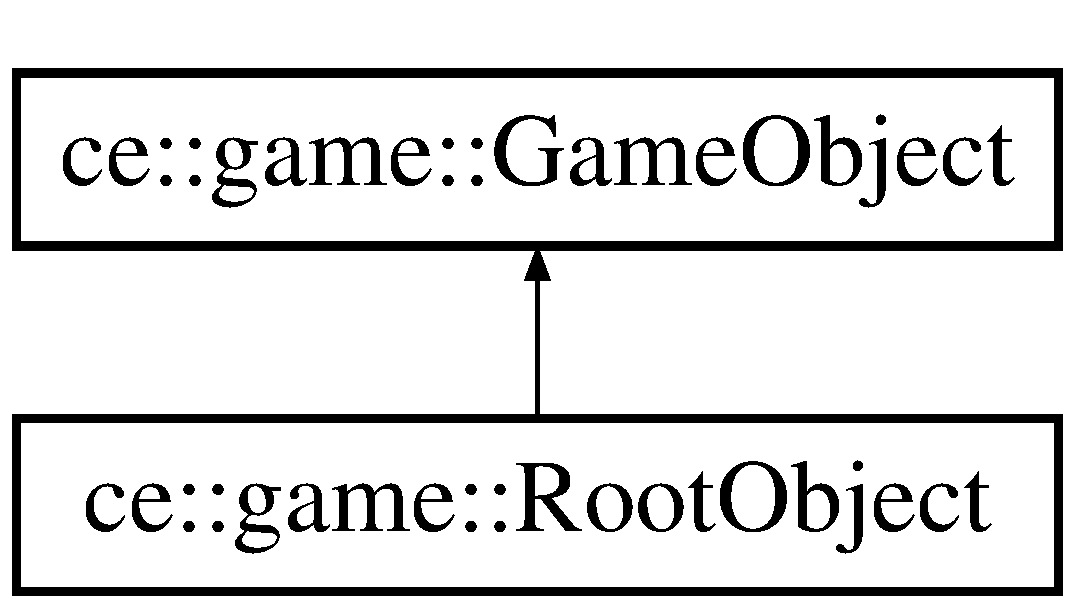
\includegraphics[height=2.000000cm]{classce_1_1game_1_1_game_object}
\end{center}
\end{figure}
\subsection*{Public Member Functions}
\begin{DoxyCompactItemize}
\item 
\mbox{\Hypertarget{classce_1_1game_1_1_game_object_a38079a556bd77da1c43d53b092b975ed}\label{classce_1_1game_1_1_game_object_a38079a556bd77da1c43d53b092b975ed}} 
\hyperlink{classce_1_1game_1_1_game_object_a38079a556bd77da1c43d53b092b975ed}{Game\+Object} ()
\begin{DoxyCompactList}\small\item\em Default constructor is only used by the root object. \end{DoxyCompactList}\item 
\mbox{\Hypertarget{classce_1_1game_1_1_game_object_a7405cbc0222f54df18d7524c6c4b0e54}\label{classce_1_1game_1_1_game_object_a7405cbc0222f54df18d7524c6c4b0e54}} 
{\bfseries Game\+Object} (\hyperlink{classce_1_1game_1_1_game_object}{Game\+Object} $\ast$parent)
\item 
\mbox{\Hypertarget{classce_1_1game_1_1_game_object_a546490e03f69dc2effa118f87c3bc7d0}\label{classce_1_1game_1_1_game_object_a546490e03f69dc2effa118f87c3bc7d0}} 
{\bfseries Game\+Object} (\hyperlink{classce_1_1game_1_1_game_object}{Game\+Object} $\ast$parent, std\+::string \hyperlink{classce_1_1game_1_1_game_object_a1de1f674c70df3bbba6aefb938ad8f32}{name})
\item 
\mbox{\Hypertarget{classce_1_1game_1_1_game_object_a483e2391d1a903ef7e0a179bc7245529}\label{classce_1_1game_1_1_game_object_a483e2391d1a903ef7e0a179bc7245529}} 
void {\bfseries set\+Parent} (\hyperlink{classce_1_1game_1_1_game_object}{Game\+Object} $\ast$parent)
\item 
\mbox{\Hypertarget{classce_1_1game_1_1_game_object_a1425bed6a585dd450f8dcd7b0d91c33a}\label{classce_1_1game_1_1_game_object_a1425bed6a585dd450f8dcd7b0d91c33a}} 
void {\bfseries add\+Child} (\hyperlink{classce_1_1game_1_1_game_object}{Game\+Object} child)
\item 
void \hyperlink{classce_1_1game_1_1_game_object_ab00a9e4dcbadfa208df56e3cbed9e8d2}{remove\+Child} (std\+::string \hyperlink{classce_1_1game_1_1_game_object_a1de1f674c70df3bbba6aefb938ad8f32}{name})
\item 
void \hyperlink{classce_1_1game_1_1_game_object_ab700981d509605a9b1bef436207e5d54}{remove\+Object} (std\+::string \hyperlink{classce_1_1game_1_1_game_object_a1de1f674c70df3bbba6aefb938ad8f32}{name})
\begin{DoxyCompactList}\small\item\em Recursive function that finds the object with name and removes it. \end{DoxyCompactList}\item 
void \hyperlink{classce_1_1game_1_1_game_object_aa77b42484f1a5c0abf1d4bf1564becac}{tick} (float dt)
\item 
void \hyperlink{classce_1_1game_1_1_game_object_ad5e81a50f4472e7557ec949eb3cc9413}{draw} (\hyperlink{classce_1_1graphics_1_1_renderer3_d}{ce\+::graphics\+::\+Renderer3D} $\ast$renderer)
\begin{DoxyCompactList}\small\item\em Draws itself and its children. \end{DoxyCompactList}\item 
\hyperlink{classce_1_1game_1_1_game_object}{Game\+Object} $\ast$ \hyperlink{classce_1_1game_1_1_game_object_a2fcc1608d7c352ba88a5fcc5d99eb5e2}{get\+Game\+Object\+By\+Name} (std\+::string \hyperlink{classce_1_1game_1_1_game_object_a1de1f674c70df3bbba6aefb938ad8f32}{name})
\begin{DoxyCompactList}\small\item\em Find a object with the name. \end{DoxyCompactList}\item 
\mbox{\Hypertarget{classce_1_1game_1_1_game_object_aff7595869f54126ae6fd16d38870f7a0}\label{classce_1_1game_1_1_game_object_aff7595869f54126ae6fd16d38870f7a0}} 
void {\bfseries add\+Component} (\hyperlink{classce_1_1game_1_1_base_component}{Base\+Component} $\ast$component)
\item 
\mbox{\Hypertarget{classce_1_1game_1_1_game_object_ac4f59a89b96dffe070a928f64ddfe382}\label{classce_1_1game_1_1_game_object_ac4f59a89b96dffe070a928f64ddfe382}} 
void {\bfseries init} ()
\end{DoxyCompactItemize}
\subsection*{Public Attributes}
\begin{DoxyCompactItemize}
\item 
\mbox{\Hypertarget{classce_1_1game_1_1_game_object_a1de1f674c70df3bbba6aefb938ad8f32}\label{classce_1_1game_1_1_game_object_a1de1f674c70df3bbba6aefb938ad8f32}} 
std\+::string \hyperlink{classce_1_1game_1_1_game_object_a1de1f674c70df3bbba6aefb938ad8f32}{name}
\begin{DoxyCompactList}\small\item\em This Game\+Objects identifier. \end{DoxyCompactList}\end{DoxyCompactItemize}
\subsection*{Protected Attributes}
\begin{DoxyCompactItemize}
\item 
\mbox{\Hypertarget{classce_1_1game_1_1_game_object_aaf7f530f3f33f9de4d688e5680ecb89b}\label{classce_1_1game_1_1_game_object_aaf7f530f3f33f9de4d688e5680ecb89b}} 
std\+::vector$<$ \hyperlink{classce_1_1game_1_1_game_object}{Game\+Object} $>$ {\bfseries m\+\_\+children}
\item 
\mbox{\Hypertarget{classce_1_1game_1_1_game_object_a93aa7c45a4e23b65ebbb3aa3d79d34a6}\label{classce_1_1game_1_1_game_object_a93aa7c45a4e23b65ebbb3aa3d79d34a6}} 
\hyperlink{classce_1_1game_1_1_game_object}{Game\+Object} $\ast$ {\bfseries m\+\_\+parent} = nullptr
\item 
\mbox{\Hypertarget{classce_1_1game_1_1_game_object_a43334ef901188cf677db3be5bcad6766}\label{classce_1_1game_1_1_game_object_a43334ef901188cf677db3be5bcad6766}} 
std\+::vector$<$ \hyperlink{classce_1_1game_1_1_base_component}{Base\+Component} $\ast$ $>$ {\bfseries m\+\_\+components}
\end{DoxyCompactItemize}


\subsection{Member Function Documentation}
\mbox{\Hypertarget{classce_1_1game_1_1_game_object_ad5e81a50f4472e7557ec949eb3cc9413}\label{classce_1_1game_1_1_game_object_ad5e81a50f4472e7557ec949eb3cc9413}} 
\index{ce\+::game\+::\+Game\+Object@{ce\+::game\+::\+Game\+Object}!draw@{draw}}
\index{draw@{draw}!ce\+::game\+::\+Game\+Object@{ce\+::game\+::\+Game\+Object}}
\subsubsection{\texorpdfstring{draw()}{draw()}}
{\footnotesize\ttfamily void ce\+::game\+::\+Game\+Object\+::draw (\begin{DoxyParamCaption}\item[{\hyperlink{classce_1_1graphics_1_1_renderer3_d}{ce\+::graphics\+::\+Renderer3D} $\ast$}]{renderer }\end{DoxyParamCaption})}



Draws itself and its children. 


\begin{DoxyParams}{Parameters}
{\em renderer} & A 3D renderer \\
\hline
\end{DoxyParams}
\mbox{\Hypertarget{classce_1_1game_1_1_game_object_a2fcc1608d7c352ba88a5fcc5d99eb5e2}\label{classce_1_1game_1_1_game_object_a2fcc1608d7c352ba88a5fcc5d99eb5e2}} 
\index{ce\+::game\+::\+Game\+Object@{ce\+::game\+::\+Game\+Object}!get\+Game\+Object\+By\+Name@{get\+Game\+Object\+By\+Name}}
\index{get\+Game\+Object\+By\+Name@{get\+Game\+Object\+By\+Name}!ce\+::game\+::\+Game\+Object@{ce\+::game\+::\+Game\+Object}}
\subsubsection{\texorpdfstring{get\+Game\+Object\+By\+Name()}{getGameObjectByName()}}
{\footnotesize\ttfamily \hyperlink{classce_1_1game_1_1_game_object}{ce\+::game\+::\+Game\+Object} $\ast$ ce\+::game\+::\+Game\+Object\+::get\+Game\+Object\+By\+Name (\begin{DoxyParamCaption}\item[{std\+::string}]{name }\end{DoxyParamCaption})}



Find a object with the name. 

It looks through it\textquotesingle{}s children to find one with the matching name, if it can\textquotesingle{}t find it it checks their children and so on.


\begin{DoxyParams}{Parameters}
{\em name} & The name of the object to look for \\
\hline
\end{DoxyParams}
\begin{DoxyReturn}{Returns}
Pointer to that game object, or nullptr if it can\textquotesingle{}t be found 
\end{DoxyReturn}
\mbox{\Hypertarget{classce_1_1game_1_1_game_object_ab00a9e4dcbadfa208df56e3cbed9e8d2}\label{classce_1_1game_1_1_game_object_ab00a9e4dcbadfa208df56e3cbed9e8d2}} 
\index{ce\+::game\+::\+Game\+Object@{ce\+::game\+::\+Game\+Object}!remove\+Child@{remove\+Child}}
\index{remove\+Child@{remove\+Child}!ce\+::game\+::\+Game\+Object@{ce\+::game\+::\+Game\+Object}}
\subsubsection{\texorpdfstring{remove\+Child()}{removeChild()}}
{\footnotesize\ttfamily void ce\+::game\+::\+Game\+Object\+::remove\+Child (\begin{DoxyParamCaption}\item[{std\+::string}]{name }\end{DoxyParamCaption})}

Remove this objects child with name

Does not affect this objects children


\begin{DoxyParams}{Parameters}
{\em name} & The name of the object \\
\hline
\end{DoxyParams}
\mbox{\Hypertarget{classce_1_1game_1_1_game_object_ab700981d509605a9b1bef436207e5d54}\label{classce_1_1game_1_1_game_object_ab700981d509605a9b1bef436207e5d54}} 
\index{ce\+::game\+::\+Game\+Object@{ce\+::game\+::\+Game\+Object}!remove\+Object@{remove\+Object}}
\index{remove\+Object@{remove\+Object}!ce\+::game\+::\+Game\+Object@{ce\+::game\+::\+Game\+Object}}
\subsubsection{\texorpdfstring{remove\+Object()}{removeObject()}}
{\footnotesize\ttfamily void ce\+::game\+::\+Game\+Object\+::remove\+Object (\begin{DoxyParamCaption}\item[{std\+::string}]{name }\end{DoxyParamCaption})}



Recursive function that finds the object with name and removes it. 

Also checks the children.


\begin{DoxyParams}{Parameters}
{\em name} & The name of the desired object \\
\hline
\end{DoxyParams}
\mbox{\Hypertarget{classce_1_1game_1_1_game_object_aa77b42484f1a5c0abf1d4bf1564becac}\label{classce_1_1game_1_1_game_object_aa77b42484f1a5c0abf1d4bf1564becac}} 
\index{ce\+::game\+::\+Game\+Object@{ce\+::game\+::\+Game\+Object}!tick@{tick}}
\index{tick@{tick}!ce\+::game\+::\+Game\+Object@{ce\+::game\+::\+Game\+Object}}
\subsubsection{\texorpdfstring{tick()}{tick()}}
{\footnotesize\ttfamily void ce\+::game\+::\+Game\+Object\+::tick (\begin{DoxyParamCaption}\item[{float}]{dt }\end{DoxyParamCaption})}

Ticks itself and its children


\begin{DoxyParams}{Parameters}
{\em dt} & Delta time \\
\hline
\end{DoxyParams}


The documentation for this class was generated from the following files\+:\begin{DoxyCompactItemize}
\item 
E\+:/\+Development/\+Game\+Engine/\+C\+Engine/src/\+Game/Game\+Object.\+h\item 
E\+:/\+Development/\+Game\+Engine/\+C\+Engine/src/\+Game/Game\+Object.\+cpp\end{DoxyCompactItemize}

\hypertarget{classce_1_1core_1_1_input}{}\section{ce\+:\+:core\+:\+:Input Class Reference}
\label{classce_1_1core_1_1_input}\index{ce\+::core\+::\+Input@{ce\+::core\+::\+Input}}


Class for handling user input.  




{\ttfamily \#include $<$Input.\+h$>$}

\subsection*{Public Member Functions}
\begin{DoxyCompactItemize}
\item 
void \hyperlink{classce_1_1core_1_1_input_aa921d892488a1c346539aab31343ac0c}{check\+Input} (const S\+D\+L\+\_\+\+Event \&e)
\item 
void \hyperlink{classce_1_1core_1_1_input_a84f905f6bd9f450d26fd23e1f8868dcb}{clear\+Button\+Binds} ()
\item 
void \hyperlink{classce_1_1core_1_1_input_a945216b48170e96f34f99c00ebeb138a}{clear\+Axis\+Binds} ()
\item 
{\footnotesize template$<$class T $>$ }\\void \hyperlink{classce_1_1core_1_1_input_a97f7ebd9ae572b447631bd05a782b73b}{bind\+Button\+Event} (\hyperlink{_input_codes_8h_a0205e42a827583bec00e09861c1bd835}{Key\+Codes} key, T $\ast$instance, void(T\+::$\ast$func)(bool))
\begin{DoxyCompactList}\small\item\em Register a button event to a callback. \end{DoxyCompactList}\item 
{\footnotesize template$<$class T $>$ }\\void \hyperlink{classce_1_1core_1_1_input_abf2973ba66d676fa5c0c731913049555}{bind\+Axis\+Event} (\hyperlink{_input_codes_8h_a9044fffd6a7c3417b0a100f0a0427a90}{Axis\+Event\+Codes} axis, T $\ast$instance, void(T\+::$\ast$func)(float))
\begin{DoxyCompactList}\small\item\em Register a axis event to a callback. \end{DoxyCompactList}\end{DoxyCompactItemize}


\subsection{Detailed Description}
Class for handling user input. 

Class for handling user input through a callback system. 

\subsection{Member Function Documentation}
\mbox{\Hypertarget{classce_1_1core_1_1_input_abf2973ba66d676fa5c0c731913049555}\label{classce_1_1core_1_1_input_abf2973ba66d676fa5c0c731913049555}} 
\index{ce\+::core\+::\+Input@{ce\+::core\+::\+Input}!bind\+Axis\+Event@{bind\+Axis\+Event}}
\index{bind\+Axis\+Event@{bind\+Axis\+Event}!ce\+::core\+::\+Input@{ce\+::core\+::\+Input}}
\subsubsection{\texorpdfstring{bind\+Axis\+Event()}{bindAxisEvent()}}
{\footnotesize\ttfamily template$<$class T $>$ \\
void ce\+::core\+::\+Input\+::bind\+Axis\+Event (\begin{DoxyParamCaption}\item[{\hyperlink{_input_codes_8h_a9044fffd6a7c3417b0a100f0a0427a90}{Axis\+Event\+Codes}}]{axis,  }\item[{T $\ast$}]{instance,  }\item[{void(T\+::$\ast$)(float)}]{func }\end{DoxyParamCaption})\hspace{0.3cm}{\ttfamily [inline]}}



Register a axis event to a callback. 


\begin{DoxyParams}{Parameters}
{\em key} & Axis\+Event\+Code to identify callback with \\
\hline
{\em instance} & Class instance which contains the function \\
\hline
{\em func} & A function pointer, function must have a float parameter and returntype void (eg\+: \&A\+Class\+::\+Function) \\
\hline
\end{DoxyParams}
\mbox{\Hypertarget{classce_1_1core_1_1_input_a97f7ebd9ae572b447631bd05a782b73b}\label{classce_1_1core_1_1_input_a97f7ebd9ae572b447631bd05a782b73b}} 
\index{ce\+::core\+::\+Input@{ce\+::core\+::\+Input}!bind\+Button\+Event@{bind\+Button\+Event}}
\index{bind\+Button\+Event@{bind\+Button\+Event}!ce\+::core\+::\+Input@{ce\+::core\+::\+Input}}
\subsubsection{\texorpdfstring{bind\+Button\+Event()}{bindButtonEvent()}}
{\footnotesize\ttfamily template$<$class T $>$ \\
void ce\+::core\+::\+Input\+::bind\+Button\+Event (\begin{DoxyParamCaption}\item[{\hyperlink{_input_codes_8h_a0205e42a827583bec00e09861c1bd835}{Key\+Codes}}]{key,  }\item[{T $\ast$}]{instance,  }\item[{void(T\+::$\ast$)(bool)}]{func }\end{DoxyParamCaption})\hspace{0.3cm}{\ttfamily [inline]}}



Register a button event to a callback. 


\begin{DoxyParams}{Parameters}
{\em key} & Keycode to identify callback with \\
\hline
{\em instance} & Class instance which contains the function \\
\hline
{\em func} & A function pointer, function must have a bool parameter and returntype void (eg\+: \&A\+Class\+::\+Function) \\
\hline
\end{DoxyParams}
\mbox{\Hypertarget{classce_1_1core_1_1_input_aa921d892488a1c346539aab31343ac0c}\label{classce_1_1core_1_1_input_aa921d892488a1c346539aab31343ac0c}} 
\index{ce\+::core\+::\+Input@{ce\+::core\+::\+Input}!check\+Input@{check\+Input}}
\index{check\+Input@{check\+Input}!ce\+::core\+::\+Input@{ce\+::core\+::\+Input}}
\subsubsection{\texorpdfstring{check\+Input()}{checkInput()}}
{\footnotesize\ttfamily void ce\+::core\+::\+Input\+::check\+Input (\begin{DoxyParamCaption}\item[{const S\+D\+L\+\_\+\+Event \&}]{e }\end{DoxyParamCaption})}

Polls input and calls callbacks \mbox{\Hypertarget{classce_1_1core_1_1_input_a945216b48170e96f34f99c00ebeb138a}\label{classce_1_1core_1_1_input_a945216b48170e96f34f99c00ebeb138a}} 
\index{ce\+::core\+::\+Input@{ce\+::core\+::\+Input}!clear\+Axis\+Binds@{clear\+Axis\+Binds}}
\index{clear\+Axis\+Binds@{clear\+Axis\+Binds}!ce\+::core\+::\+Input@{ce\+::core\+::\+Input}}
\subsubsection{\texorpdfstring{clear\+Axis\+Binds()}{clearAxisBinds()}}
{\footnotesize\ttfamily void ce\+::core\+::\+Input\+::clear\+Axis\+Binds (\begin{DoxyParamCaption}{ }\end{DoxyParamCaption})}

Completely clear the axis bindings \mbox{\Hypertarget{classce_1_1core_1_1_input_a84f905f6bd9f450d26fd23e1f8868dcb}\label{classce_1_1core_1_1_input_a84f905f6bd9f450d26fd23e1f8868dcb}} 
\index{ce\+::core\+::\+Input@{ce\+::core\+::\+Input}!clear\+Button\+Binds@{clear\+Button\+Binds}}
\index{clear\+Button\+Binds@{clear\+Button\+Binds}!ce\+::core\+::\+Input@{ce\+::core\+::\+Input}}
\subsubsection{\texorpdfstring{clear\+Button\+Binds()}{clearButtonBinds()}}
{\footnotesize\ttfamily void ce\+::core\+::\+Input\+::clear\+Button\+Binds (\begin{DoxyParamCaption}{ }\end{DoxyParamCaption})}

Completely clear the button bindings 

The documentation for this class was generated from the following files\+:\begin{DoxyCompactItemize}
\item 
E\+:/\+Development/\+Game\+Engine/\+C\+Engine/src/\+Core/\hyperlink{_input_8h}{Input.\+h}\item 
E\+:/\+Development/\+Game\+Engine/\+C\+Engine/src/\+Core/Input.\+cpp\end{DoxyCompactItemize}

\hypertarget{structce_1_1core_1_1_joystick}{}\section{ce\+:\+:core\+:\+:Joystick Struct Reference}
\label{structce_1_1core_1_1_joystick}\index{ce\+::core\+::\+Joystick@{ce\+::core\+::\+Joystick}}


Structure containing information needed for Joysticks and Controllers.  




{\ttfamily \#include $<$Input.\+h$>$}

\subsection*{Public Attributes}
\begin{DoxyCompactItemize}
\item 
\mbox{\Hypertarget{structce_1_1core_1_1_joystick_a91d7c9adbb3e74b6e6379e50ff71c7b9}\label{structce_1_1core_1_1_joystick_a91d7c9adbb3e74b6e6379e50ff71c7b9}} 
int {\bfseries instance\+ID} = 0
\item 
\mbox{\Hypertarget{structce_1_1core_1_1_joystick_a7d8e4662b79ba8cf85ada42f146d0cb9}\label{structce_1_1core_1_1_joystick_a7d8e4662b79ba8cf85ada42f146d0cb9}} 
S\+D\+L\+\_\+\+Joystick $\ast$ {\bfseries joystick} = nullptr
\item 
\mbox{\Hypertarget{structce_1_1core_1_1_joystick_a4becd96a25a7cfc34e53abde7b948810}\label{structce_1_1core_1_1_joystick_a4becd96a25a7cfc34e53abde7b948810}} 
S\+D\+L\+\_\+\+Game\+Controller $\ast$ {\bfseries controller} = nullptr
\end{DoxyCompactItemize}


\subsection{Detailed Description}
Structure containing information needed for Joysticks and Controllers. 

The documentation for this struct was generated from the following file\+:\begin{DoxyCompactItemize}
\item 
Core/Input.\+h\end{DoxyCompactItemize}

\hypertarget{structce_1_1graphics_1_1_light_setup}{}\section{ce\+:\+:graphics\+:\+:Light\+Setup Struct Reference}
\label{structce_1_1graphics_1_1_light_setup}\index{ce\+::graphics\+::\+Light\+Setup@{ce\+::graphics\+::\+Light\+Setup}}


Structure representing a setup of lights that we can easily give to the renderers.  




{\ttfamily \#include $<$Lights.\+h$>$}

\subsection*{Public Attributes}
\begin{DoxyCompactItemize}
\item 
\mbox{\Hypertarget{structce_1_1graphics_1_1_light_setup_a244f07e42597b634054c7c1b7733054d}\label{structce_1_1graphics_1_1_light_setup_a244f07e42597b634054c7c1b7733054d}} 
std\+::vector$<$ \hyperlink{classce_1_1graphics_1_1_dir_light}{Dir\+Light} $>$ {\bfseries dir\+Lights}
\item 
\mbox{\Hypertarget{structce_1_1graphics_1_1_light_setup_aed06cdb1ef61afd4705c26ef1781637e}\label{structce_1_1graphics_1_1_light_setup_aed06cdb1ef61afd4705c26ef1781637e}} 
std\+::vector$<$ \hyperlink{classce_1_1graphics_1_1_point_light}{Point\+Light} $>$ {\bfseries point\+Lights}
\item 
\mbox{\Hypertarget{structce_1_1graphics_1_1_light_setup_a68944c5cb6b197a32fe5bfdd89e3ed4a}\label{structce_1_1graphics_1_1_light_setup_a68944c5cb6b197a32fe5bfdd89e3ed4a}} 
std\+::vector$<$ \hyperlink{classce_1_1graphics_1_1_spot_light}{Spot\+Light} $>$ {\bfseries spot\+Lights}
\end{DoxyCompactItemize}


\subsection{Detailed Description}
Structure representing a setup of lights that we can easily give to the renderers. 

The documentation for this struct was generated from the following file\+:\begin{DoxyCompactItemize}
\item 
Graphics/\hyperlink{_lights_8h}{Lights.\+h}\end{DoxyCompactItemize}

\hypertarget{structce_1_1graphics_1_1_material}{}\section{ce\+:\+:graphics\+:\+:Material Struct Reference}
\label{structce_1_1graphics_1_1_material}\index{ce\+::graphics\+::\+Material@{ce\+::graphics\+::\+Material}}


\hyperlink{structce_1_1graphics_1_1_material}{Material} representation.  




{\ttfamily \#include $<$Material.\+h$>$}

\subsection*{Public Member Functions}
\begin{DoxyCompactItemize}
\item 
\mbox{\Hypertarget{structce_1_1graphics_1_1_material_af33c976594ddcca02b16b7fbf64d429a}\label{structce_1_1graphics_1_1_material_af33c976594ddcca02b16b7fbf64d429a}} 
bool \hyperlink{structce_1_1graphics_1_1_material_af33c976594ddcca02b16b7fbf64d429a}{has\+Property} (\hyperlink{_material_8h_aac4ec325697a8f788007e105d586d217}{Material\+Property} matprop)
\begin{DoxyCompactList}\small\item\em Checks if material has a property. \end{DoxyCompactList}\end{DoxyCompactItemize}
\subsection*{Public Attributes}
\begin{DoxyCompactItemize}
\item 
\hyperlink{classce_1_1graphics_1_1_shader}{Shader} \hyperlink{structce_1_1graphics_1_1_material_a583b33732dc9ed17a20d9d1bcd636a52}{shader}
\item 
std\+::vector$<$ \hyperlink{structce_1_1graphics_1_1_texture}{Texture} $>$ \hyperlink{structce_1_1graphics_1_1_material_ad14fc2a8d3a7d9241226471f8f2e2fcc}{textures}
\item 
float \hyperlink{structce_1_1graphics_1_1_material_a62ed7d4af263dbdd7065a9b664bfab6e}{shininess} = 32.\+0f
\item 
float \hyperlink{structce_1_1graphics_1_1_material_ad6f3a5c250e374b47ca6bbefb75b8a6c}{opacity} = 1.\+0f
\end{DoxyCompactItemize}
\subsection*{Protected Attributes}
\begin{DoxyCompactItemize}
\item 
\mbox{\Hypertarget{structce_1_1graphics_1_1_material_aff162e4070b34139c00cc149c70eb5f8}\label{structce_1_1graphics_1_1_material_aff162e4070b34139c00cc149c70eb5f8}} 
unsigned int {\bfseries m\+\_\+material\+Properties} = 0
\end{DoxyCompactItemize}
\subsection*{Friends}
\begin{DoxyCompactItemize}
\item 
\mbox{\Hypertarget{structce_1_1graphics_1_1_material_ac22dade55c1e8f81ea3e0892cd321190}\label{structce_1_1graphics_1_1_material_ac22dade55c1e8f81ea3e0892cd321190}} 
class {\bfseries Model\+Loader}
\end{DoxyCompactItemize}


\subsection{Detailed Description}
\hyperlink{structce_1_1graphics_1_1_material}{Material} representation. 

\subsection{Member Data Documentation}
\mbox{\Hypertarget{structce_1_1graphics_1_1_material_ad6f3a5c250e374b47ca6bbefb75b8a6c}\label{structce_1_1graphics_1_1_material_ad6f3a5c250e374b47ca6bbefb75b8a6c}} 
\index{ce\+::graphics\+::\+Material@{ce\+::graphics\+::\+Material}!opacity@{opacity}}
\index{opacity@{opacity}!ce\+::graphics\+::\+Material@{ce\+::graphics\+::\+Material}}
\subsubsection{\texorpdfstring{opacity}{opacity}}
{\footnotesize\ttfamily float ce\+::graphics\+::\+Material\+::opacity = 1.\+0f}

The opacity of the object \mbox{\Hypertarget{structce_1_1graphics_1_1_material_a583b33732dc9ed17a20d9d1bcd636a52}\label{structce_1_1graphics_1_1_material_a583b33732dc9ed17a20d9d1bcd636a52}} 
\index{ce\+::graphics\+::\+Material@{ce\+::graphics\+::\+Material}!shader@{shader}}
\index{shader@{shader}!ce\+::graphics\+::\+Material@{ce\+::graphics\+::\+Material}}
\subsubsection{\texorpdfstring{shader}{shader}}
{\footnotesize\ttfamily \hyperlink{classce_1_1graphics_1_1_shader}{Shader} ce\+::graphics\+::\+Material\+::shader}

\hyperlink{classce_1_1graphics_1_1_shader}{Shader} used to draw the material \mbox{\Hypertarget{structce_1_1graphics_1_1_material_a62ed7d4af263dbdd7065a9b664bfab6e}\label{structce_1_1graphics_1_1_material_a62ed7d4af263dbdd7065a9b664bfab6e}} 
\index{ce\+::graphics\+::\+Material@{ce\+::graphics\+::\+Material}!shininess@{shininess}}
\index{shininess@{shininess}!ce\+::graphics\+::\+Material@{ce\+::graphics\+::\+Material}}
\subsubsection{\texorpdfstring{shininess}{shininess}}
{\footnotesize\ttfamily float ce\+::graphics\+::\+Material\+::shininess = 32.\+0f}

The shininess of the material \mbox{\Hypertarget{structce_1_1graphics_1_1_material_ad14fc2a8d3a7d9241226471f8f2e2fcc}\label{structce_1_1graphics_1_1_material_ad14fc2a8d3a7d9241226471f8f2e2fcc}} 
\index{ce\+::graphics\+::\+Material@{ce\+::graphics\+::\+Material}!textures@{textures}}
\index{textures@{textures}!ce\+::graphics\+::\+Material@{ce\+::graphics\+::\+Material}}
\subsubsection{\texorpdfstring{textures}{textures}}
{\footnotesize\ttfamily std\+::vector$<$\hyperlink{structce_1_1graphics_1_1_texture}{Texture}$>$ ce\+::graphics\+::\+Material\+::textures}

Textures used in this material 

The documentation for this struct was generated from the following file\+:\begin{DoxyCompactItemize}
\item 
E\+:/\+Development/\+Game\+Engine/\+C\+Engine/src/\+Graphics/\+Model/\hyperlink{_material_8h}{Material.\+h}\end{DoxyCompactItemize}

\hypertarget{classce_1_1graphics_1_1_mesh}{}\section{ce\+:\+:graphics\+:\+:Mesh Class Reference}
\label{classce_1_1graphics_1_1_mesh}\index{ce\+::graphics\+::\+Mesh@{ce\+::graphics\+::\+Mesh}}


A object representation of a mesh.  




{\ttfamily \#include $<$Mesh.\+h$>$}

\subsection*{Public Member Functions}
\begin{DoxyCompactItemize}
\item 
\mbox{\Hypertarget{classce_1_1graphics_1_1_mesh_a5069371e754447217960efdf27f89069}\label{classce_1_1graphics_1_1_mesh_a5069371e754447217960efdf27f89069}} 
\hyperlink{classce_1_1graphics_1_1_mesh_a5069371e754447217960efdf27f89069}{Mesh} (\hyperlink{_vertex_8h_a72d0effc290681342d1fc2b5fffa6aef}{Vertex\+Array} vertices, \hyperlink{_vertex_8h_a25b1e42db1e356e8bfc3ab61ade25040}{Index\+Array} indices, \hyperlink{structce_1_1graphics_1_1_material}{Material} \hyperlink{classce_1_1graphics_1_1_mesh_ae10e3d9449f7af5b17644b94d2d4e396}{material})
\begin{DoxyCompactList}\small\item\em Construct mesh from a set of vertices, indices and a material. \end{DoxyCompactList}\item 
void \hyperlink{classce_1_1graphics_1_1_mesh_a4c056e83554a4face474bbc21d309910}{draw} ()
\begin{DoxyCompactList}\small\item\em Draw mesh. \end{DoxyCompactList}\end{DoxyCompactItemize}
\subsection*{Public Attributes}
\begin{DoxyCompactItemize}
\item 
\mbox{\Hypertarget{classce_1_1graphics_1_1_mesh_ae10e3d9449f7af5b17644b94d2d4e396}\label{classce_1_1graphics_1_1_mesh_ae10e3d9449f7af5b17644b94d2d4e396}} 
\hyperlink{structce_1_1graphics_1_1_material}{Material} \hyperlink{classce_1_1graphics_1_1_mesh_ae10e3d9449f7af5b17644b94d2d4e396}{material}
\begin{DoxyCompactList}\small\item\em The material used by this mesh. \end{DoxyCompactList}\end{DoxyCompactItemize}
\subsection*{Protected Attributes}
\begin{DoxyCompactItemize}
\item 
\mbox{\Hypertarget{classce_1_1graphics_1_1_mesh_a8a9d810a84babc359088216a34149004}\label{classce_1_1graphics_1_1_mesh_a8a9d810a84babc359088216a34149004}} 
unsigned int {\bfseries m\+\_\+\+V\+AO}
\item 
\mbox{\Hypertarget{classce_1_1graphics_1_1_mesh_a4b1ba8be0e3005bbe35ab9b65525f16d}\label{classce_1_1graphics_1_1_mesh_a4b1ba8be0e3005bbe35ab9b65525f16d}} 
unsigned int {\bfseries m\+\_\+\+V\+BO}
\item 
\mbox{\Hypertarget{classce_1_1graphics_1_1_mesh_a40681c51b3147e18129b82b768ff935e}\label{classce_1_1graphics_1_1_mesh_a40681c51b3147e18129b82b768ff935e}} 
unsigned int {\bfseries m\+\_\+\+E\+BO}
\item 
\mbox{\Hypertarget{classce_1_1graphics_1_1_mesh_a7ef8ad299b4f4c9d9488f6c547d4fd7e}\label{classce_1_1graphics_1_1_mesh_a7ef8ad299b4f4c9d9488f6c547d4fd7e}} 
\hyperlink{_vertex_8h_a72d0effc290681342d1fc2b5fffa6aef}{Vertex\+Array} {\bfseries m\+\_\+vertices}
\item 
\mbox{\Hypertarget{classce_1_1graphics_1_1_mesh_a94287f8ee272274fe7ee4a6716f2c509}\label{classce_1_1graphics_1_1_mesh_a94287f8ee272274fe7ee4a6716f2c509}} 
\hyperlink{_vertex_8h_a25b1e42db1e356e8bfc3ab61ade25040}{Index\+Array} {\bfseries m\+\_\+indices}
\item 
\mbox{\Hypertarget{classce_1_1graphics_1_1_mesh_aa6598a29dc63d2e99adc85b78168c675}\label{classce_1_1graphics_1_1_mesh_aa6598a29dc63d2e99adc85b78168c675}} 
std\+::string {\bfseries m\+\_\+name}
\end{DoxyCompactItemize}
\subsection*{Friends}
\begin{DoxyCompactItemize}
\item 
\mbox{\Hypertarget{classce_1_1graphics_1_1_mesh_ac22dade55c1e8f81ea3e0892cd321190}\label{classce_1_1graphics_1_1_mesh_ac22dade55c1e8f81ea3e0892cd321190}} 
class {\bfseries Model\+Loader}
\end{DoxyCompactItemize}


\subsection{Detailed Description}
A object representation of a mesh. 

\subsection{Member Function Documentation}
\mbox{\Hypertarget{classce_1_1graphics_1_1_mesh_a4c056e83554a4face474bbc21d309910}\label{classce_1_1graphics_1_1_mesh_a4c056e83554a4face474bbc21d309910}} 
\index{ce\+::graphics\+::\+Mesh@{ce\+::graphics\+::\+Mesh}!draw@{draw}}
\index{draw@{draw}!ce\+::graphics\+::\+Mesh@{ce\+::graphics\+::\+Mesh}}
\subsubsection{\texorpdfstring{draw()}{draw()}}
{\footnotesize\ttfamily void ce\+::graphics\+::\+Mesh\+::draw (\begin{DoxyParamCaption}{ }\end{DoxyParamCaption})}



Draw mesh. 

To be updated currently very slow 

The documentation for this class was generated from the following files\+:\begin{DoxyCompactItemize}
\item 
E\+:/\+Development/\+Game\+Engine/\+C\+Engine/src/\+Graphics/\+Model/\hyperlink{_mesh_8h}{Mesh.\+h}\item 
E\+:/\+Development/\+Game\+Engine/\+C\+Engine/src/\+Graphics/\+Model/Mesh.\+cpp\end{DoxyCompactItemize}

\hypertarget{classce_1_1graphics_1_1_model}{}\section{ce\+:\+:graphics\+:\+:Model Class Reference}
\label{classce_1_1graphics_1_1_model}\index{ce\+::graphics\+::\+Model@{ce\+::graphics\+::\+Model}}
\subsection*{Public Member Functions}
\begin{DoxyCompactItemize}
\item 
\mbox{\Hypertarget{classce_1_1graphics_1_1_model_ae80b6da77f07543d9d423ca4884c63d1}\label{classce_1_1graphics_1_1_model_ae80b6da77f07543d9d423ca4884c63d1}} 
{\bfseries Model} (std\+::vector$<$ std\+::shared\+\_\+ptr$<$ \hyperlink{classce_1_1graphics_1_1_mesh}{Mesh} $>$$>$ meshes)
\item 
\mbox{\Hypertarget{classce_1_1graphics_1_1_model_a32e4b5c3880eec770dabd21f8b053d49}\label{classce_1_1graphics_1_1_model_a32e4b5c3880eec770dabd21f8b053d49}} 
void {\bfseries draw} ()
\item 
\mbox{\Hypertarget{classce_1_1graphics_1_1_model_a7bc6f7fd875dbfadc56576815c85844c}\label{classce_1_1graphics_1_1_model_a7bc6f7fd875dbfadc56576815c85844c}} 
void {\bfseries draw} (\hyperlink{classce_1_1graphics_1_1_forward_renderer}{Forward\+Renderer} $\ast$renderer, glm\+::mat4 model\+Matrix)
\end{DoxyCompactItemize}
\subsection*{Protected Attributes}
\begin{DoxyCompactItemize}
\item 
\mbox{\Hypertarget{classce_1_1graphics_1_1_model_a326b8332797594d1c5bb18ddb0e8d953}\label{classce_1_1graphics_1_1_model_a326b8332797594d1c5bb18ddb0e8d953}} 
std\+::string {\bfseries m\+\_\+directory}
\item 
\mbox{\Hypertarget{classce_1_1graphics_1_1_model_a03d7857dc5c72c845ff0664ac2abc2ec}\label{classce_1_1graphics_1_1_model_a03d7857dc5c72c845ff0664ac2abc2ec}} 
std\+::vector$<$ std\+::shared\+\_\+ptr$<$ \hyperlink{classce_1_1graphics_1_1_mesh}{Mesh} $>$ $>$ {\bfseries m\+\_\+meshes}
\end{DoxyCompactItemize}
\subsection*{Friends}
\begin{DoxyCompactItemize}
\item 
\mbox{\Hypertarget{classce_1_1graphics_1_1_model_ac22dade55c1e8f81ea3e0892cd321190}\label{classce_1_1graphics_1_1_model_ac22dade55c1e8f81ea3e0892cd321190}} 
class {\bfseries Model\+Loader}
\end{DoxyCompactItemize}


The documentation for this class was generated from the following files\+:\begin{DoxyCompactItemize}
\item 
Graphics/\+Model/Model.\+h\item 
Graphics/\+Model/Model.\+cpp\end{DoxyCompactItemize}

\hypertarget{classce_1_1game_1_1_model_component}{}\section{ce\+:\+:game\+:\+:Model\+Component Class Reference}
\label{classce_1_1game_1_1_model_component}\index{ce\+::game\+::\+Model\+Component@{ce\+::game\+::\+Model\+Component}}
Inheritance diagram for ce\+:\+:game\+:\+:Model\+Component\+:\begin{figure}[H]
\begin{center}
\leavevmode
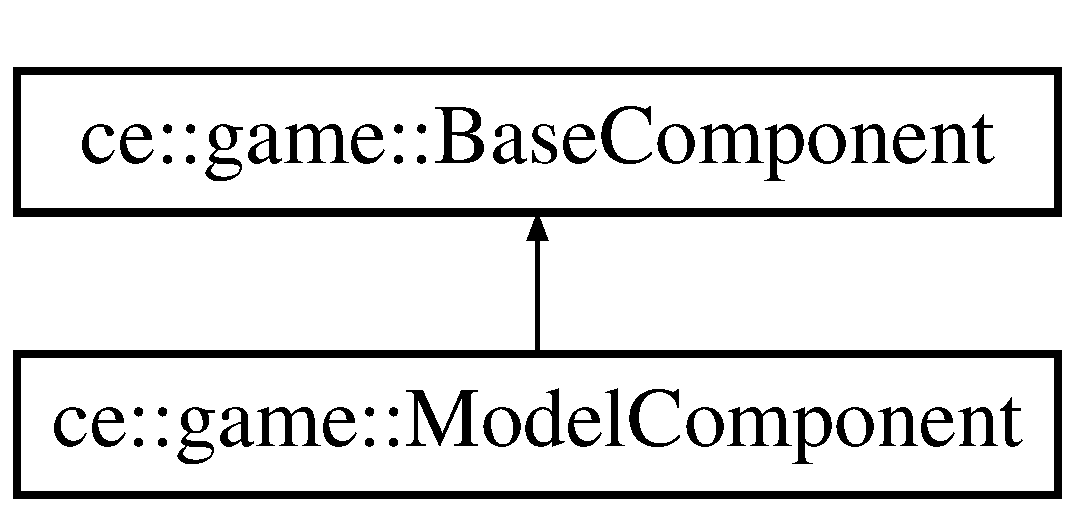
\includegraphics[height=2.000000cm]{classce_1_1game_1_1_model_component}
\end{center}
\end{figure}
\subsection*{Public Member Functions}
\begin{DoxyCompactItemize}
\item 
\mbox{\Hypertarget{classce_1_1game_1_1_model_component_afbfe9e210796b98160700daea8fd7946}\label{classce_1_1game_1_1_model_component_afbfe9e210796b98160700daea8fd7946}} 
virtual void {\bfseries init} () override
\item 
\mbox{\Hypertarget{classce_1_1game_1_1_model_component_a36b54a8ccafa5144204671429c490a9a}\label{classce_1_1game_1_1_model_component_a36b54a8ccafa5144204671429c490a9a}} 
virtual void {\bfseries tick} (float dt) override
\item 
\mbox{\Hypertarget{classce_1_1game_1_1_model_component_aed3b814d2bdb0fb99cb280d963379d67}\label{classce_1_1game_1_1_model_component_aed3b814d2bdb0fb99cb280d963379d67}} 
virtual void {\bfseries draw} (\hyperlink{classce_1_1graphics_1_1_renderer3_d}{ce\+::graphics\+::\+Renderer3D} $\ast$renderer) override
\item 
virtual std\+::string \hyperlink{classce_1_1game_1_1_model_component_aaac15cad336e35df7be55dda34f53643}{get\+Type} () override
\begin{DoxyCompactList}\small\item\em Returns the type of Component in a string value. \end{DoxyCompactList}\item 
\mbox{\Hypertarget{classce_1_1game_1_1_model_component_addc52f099ee60e0018af78c2c98a8751}\label{classce_1_1game_1_1_model_component_addc52f099ee60e0018af78c2c98a8751}} 
void {\bfseries set\+Model} (\hyperlink{classce_1_1graphics_1_1_model}{ce\+::graphics\+::\+Model} model)
\end{DoxyCompactItemize}
\subsection*{Protected Attributes}
\begin{DoxyCompactItemize}
\item 
\mbox{\Hypertarget{classce_1_1game_1_1_model_component_a275f61abbf878c431026539adf141775}\label{classce_1_1game_1_1_model_component_a275f61abbf878c431026539adf141775}} 
\hyperlink{classce_1_1graphics_1_1_model}{ce\+::graphics\+::\+Model} {\bfseries m\+\_\+model}
\end{DoxyCompactItemize}
\subsection*{Additional Inherited Members}


\subsection{Member Function Documentation}
\mbox{\Hypertarget{classce_1_1game_1_1_model_component_aaac15cad336e35df7be55dda34f53643}\label{classce_1_1game_1_1_model_component_aaac15cad336e35df7be55dda34f53643}} 
\index{ce\+::game\+::\+Model\+Component@{ce\+::game\+::\+Model\+Component}!get\+Type@{get\+Type}}
\index{get\+Type@{get\+Type}!ce\+::game\+::\+Model\+Component@{ce\+::game\+::\+Model\+Component}}
\subsubsection{\texorpdfstring{get\+Type()}{getType()}}
{\footnotesize\ttfamily std\+::string ce\+::game\+::\+Model\+Component\+::get\+Type (\begin{DoxyParamCaption}{ }\end{DoxyParamCaption})\hspace{0.3cm}{\ttfamily [override]}, {\ttfamily [virtual]}}



Returns the type of Component in a string value. 

Example\+: Model, Transform etc 

Implements \hyperlink{classce_1_1game_1_1_base_component_a1022b55c1926a019a2b3a71fb6b9150e}{ce\+::game\+::\+Base\+Component}.



The documentation for this class was generated from the following files\+:\begin{DoxyCompactItemize}
\item 
E\+:/\+Development/\+Game\+Engine/\+C\+Engine/src/\+Game/\+Components/Model\+Component.\+h\item 
E\+:/\+Development/\+Game\+Engine/\+C\+Engine/src/\+Game/\+Components/Model\+Component.\+cpp\end{DoxyCompactItemize}

\hypertarget{classce_1_1graphics_1_1_model_loader}{}\section{ce\+:\+:graphics\+:\+:Model\+Loader Class Reference}
\label{classce_1_1graphics_1_1_model_loader}\index{ce\+::graphics\+::\+Model\+Loader@{ce\+::graphics\+::\+Model\+Loader}}


Loads models.  




{\ttfamily \#include $<$Model\+Loader.\+h$>$}

\subsection*{Public Member Functions}
\begin{DoxyCompactItemize}
\item 
\hyperlink{classce_1_1graphics_1_1_model}{Model} \hyperlink{classce_1_1graphics_1_1_model_loader_aee7761094a5e10a81555b4a695a55043}{load\+Model} (std\+::string path)
\begin{DoxyCompactList}\small\item\em Load a model. \end{DoxyCompactList}\end{DoxyCompactItemize}


\subsection{Detailed Description}
Loads models. 

Loads and contains the original models Keeps track of duplicates 

\subsection{Member Function Documentation}
\mbox{\Hypertarget{classce_1_1graphics_1_1_model_loader_aee7761094a5e10a81555b4a695a55043}\label{classce_1_1graphics_1_1_model_loader_aee7761094a5e10a81555b4a695a55043}} 
\index{ce\+::graphics\+::\+Model\+Loader@{ce\+::graphics\+::\+Model\+Loader}!load\+Model@{load\+Model}}
\index{load\+Model@{load\+Model}!ce\+::graphics\+::\+Model\+Loader@{ce\+::graphics\+::\+Model\+Loader}}
\subsubsection{\texorpdfstring{load\+Model()}{loadModel()}}
{\footnotesize\ttfamily \hyperlink{classce_1_1graphics_1_1_model}{ce\+::graphics\+::\+Model} ce\+::graphics\+::\+Model\+Loader\+::load\+Model (\begin{DoxyParamCaption}\item[{std\+::string}]{path }\end{DoxyParamCaption})}



Load a model. 


\begin{DoxyParams}{Parameters}
{\em path} & Path to model file (eg\+: a .obj file) \\
\hline
\end{DoxyParams}


The documentation for this class was generated from the following files\+:\begin{DoxyCompactItemize}
\item 
E\+:/\+Development/\+Game\+Engine/\+C\+Engine/src/\+Graphics/\+Model/\hyperlink{_model_loader_8h}{Model\+Loader.\+h}\item 
E\+:/\+Development/\+Game\+Engine/\+C\+Engine/src/\+Graphics/\+Model/Model\+Loader.\+cpp\end{DoxyCompactItemize}

\hypertarget{classce_1_1graphics_1_1_point_light}{}\section{ce\+:\+:graphics\+:\+:Point\+Light Class Reference}
\label{classce_1_1graphics_1_1_point_light}\index{ce\+::graphics\+::\+Point\+Light@{ce\+::graphics\+::\+Point\+Light}}


A point light.  




{\ttfamily \#include $<$Lights.\+h$>$}

Inheritance diagram for ce\+:\+:graphics\+:\+:Point\+Light\+:\begin{figure}[H]
\begin{center}
\leavevmode
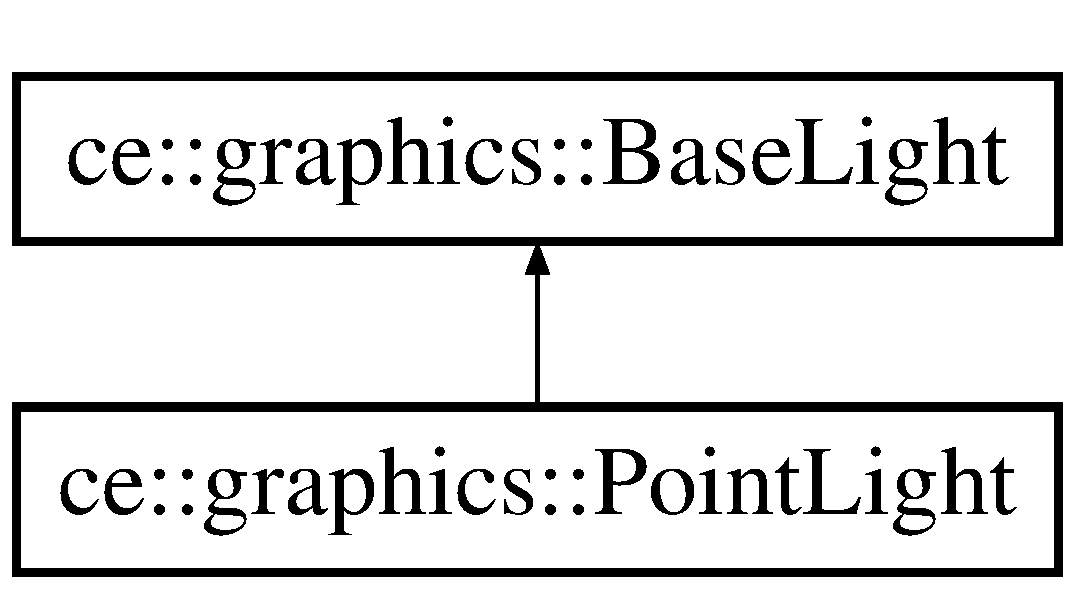
\includegraphics[height=2.000000cm]{classce_1_1graphics_1_1_point_light}
\end{center}
\end{figure}
\subsection*{Public Attributes}
\begin{DoxyCompactItemize}
\item 
\mbox{\Hypertarget{classce_1_1graphics_1_1_point_light_a243f8f1019644d4a983a76bee93dd0e5}\label{classce_1_1graphics_1_1_point_light_a243f8f1019644d4a983a76bee93dd0e5}} 
glm\+::vec3 {\bfseries position} = glm\+::vec3(0.\+0f, 0.\+0f, 0.\+0f)
\item 
\mbox{\Hypertarget{classce_1_1graphics_1_1_point_light_aeaa6b5a0295a24d5ee38857bc27fe971}\label{classce_1_1graphics_1_1_point_light_aeaa6b5a0295a24d5ee38857bc27fe971}} 
float {\bfseries constant} = 1.\+0f
\item 
\mbox{\Hypertarget{classce_1_1graphics_1_1_point_light_a17a135df574a30bc43e0ca56f46361ca}\label{classce_1_1graphics_1_1_point_light_a17a135df574a30bc43e0ca56f46361ca}} 
float {\bfseries linear} = 0.\+09f
\item 
\mbox{\Hypertarget{classce_1_1graphics_1_1_point_light_a4a5db9aa2d038c7392d386614c92ac72}\label{classce_1_1graphics_1_1_point_light_a4a5db9aa2d038c7392d386614c92ac72}} 
float {\bfseries quadratic} = 0.\+032f
\end{DoxyCompactItemize}


\subsection{Detailed Description}
A point light. 

The documentation for this class was generated from the following file\+:\begin{DoxyCompactItemize}
\item 
Graphics/\hyperlink{_lights_8h}{Lights.\+h}\end{DoxyCompactItemize}

\hypertarget{structce_1_1graphics_1_1_render_command}{}\section{ce\+:\+:graphics\+:\+:Render\+Command Struct Reference}
\label{structce_1_1graphics_1_1_render_command}\index{ce\+::graphics\+::\+Render\+Command@{ce\+::graphics\+::\+Render\+Command}}


A structure of a rendercommand to be sent to a renderer.  




{\ttfamily \#include $<$Render\+Command.\+h$>$}

\subsection*{Public Attributes}
\begin{DoxyCompactItemize}
\item 
\mbox{\Hypertarget{structce_1_1graphics_1_1_render_command_aea0982beaba0aecd4bc10f0e9f84d741}\label{structce_1_1graphics_1_1_render_command_aea0982beaba0aecd4bc10f0e9f84d741}} 
\hyperlink{classce_1_1graphics_1_1_mesh}{Mesh} $\ast$ {\bfseries mesh}
\item 
\mbox{\Hypertarget{structce_1_1graphics_1_1_render_command_a917fc9ebe6d75b747bac29e70a7fad3c}\label{structce_1_1graphics_1_1_render_command_a917fc9ebe6d75b747bac29e70a7fad3c}} 
glm\+::mat4 {\bfseries transform}
\item 
\mbox{\Hypertarget{structce_1_1graphics_1_1_render_command_a1cb0de110a1a1c7cc1ab3d8b3ec5e43b}\label{structce_1_1graphics_1_1_render_command_a1cb0de110a1a1c7cc1ab3d8b3ec5e43b}} 
\hyperlink{classce_1_1graphics_1_1_shader}{Shader} {\bfseries shader}
\end{DoxyCompactItemize}


\subsection{Detailed Description}
A structure of a rendercommand to be sent to a renderer. 

The documentation for this struct was generated from the following file\+:\begin{DoxyCompactItemize}
\item 
E\+:/\+Development/\+Game\+Engine/\+C\+Engine/src/\+Graphics/\+Renderer/\hyperlink{_render_command_8h}{Render\+Command.\+h}\end{DoxyCompactItemize}

\hypertarget{classce_1_1graphics_1_1_renderer3_d}{}\section{ce\+:\+:graphics\+:\+:Renderer3D Class Reference}
\label{classce_1_1graphics_1_1_renderer3_d}\index{ce\+::graphics\+::\+Renderer3D@{ce\+::graphics\+::\+Renderer3D}}


{\ttfamily \#include $<$Renderer3\+D.\+h$>$}

Inheritance diagram for ce\+:\+:graphics\+:\+:Renderer3D\+:\begin{figure}[H]
\begin{center}
\leavevmode
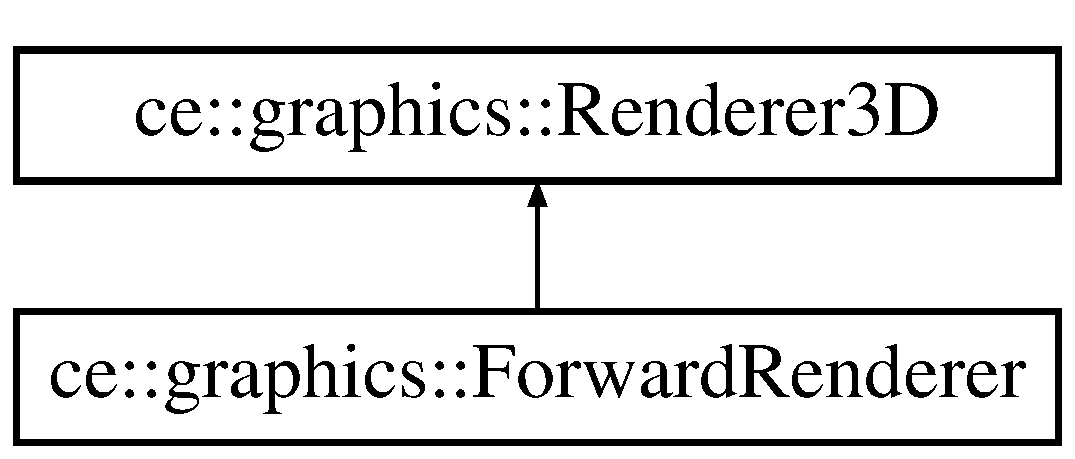
\includegraphics[height=2.000000cm]{classce_1_1graphics_1_1_renderer3_d}
\end{center}
\end{figure}
\subsection*{Public Member Functions}
\begin{DoxyCompactItemize}
\item 
virtual void \hyperlink{classce_1_1graphics_1_1_renderer3_d_ae887bbdc74af40838e6d059d30bb430b}{init} ()=0
\item 
virtual void \hyperlink{classce_1_1graphics_1_1_renderer3_d_a51818b5b581c33001ddbbc6dff9d6e36}{begin} ()=0
\item 
virtual void \hyperlink{classce_1_1graphics_1_1_renderer3_d_a94e60931e0ff3f26b217db09a11ee7e6}{begin\+Scene} (\hyperlink{classce_1_1graphics_1_1_camera}{Camera} $\ast$camera)=0
\item 
virtual void \hyperlink{classce_1_1graphics_1_1_renderer3_d_a67e956930a17600cdcfc689aa624f990}{submit} (const \hyperlink{structce_1_1graphics_1_1_render_command}{Render\+Command} \&command)=0
\item 
virtual void \hyperlink{classce_1_1graphics_1_1_renderer3_d_aba7b0abfa0aad0d89a816923e83ef787}{submit\+Mesh} (\hyperlink{classce_1_1graphics_1_1_mesh}{Mesh} $\ast$mesh, const glm\+::mat4 \&transform)=0
\item 
virtual void \hyperlink{classce_1_1graphics_1_1_renderer3_d_a4a2eb6efe3adbff611c20141159eb3dc}{submit\+Light\+Setup} (const \hyperlink{structce_1_1graphics_1_1_light_setup}{Light\+Setup} \&light\+Setup)=0
\item 
virtual void \hyperlink{classce_1_1graphics_1_1_renderer3_d_a0b8feaf1dd7f6ee03c7be2197d012e25}{end\+Scene} ()=0
\item 
virtual void \hyperlink{classce_1_1graphics_1_1_renderer3_d_a4d35e07f42a4fb42ebe3f8e57bfcdb58}{end} ()=0
\item 
virtual void \hyperlink{classce_1_1graphics_1_1_renderer3_d_a7b258350b5af957550a2d29800d3c5b7}{present} ()=0
\item 
virtual void \hyperlink{classce_1_1graphics_1_1_renderer3_d_a39b5c5b8a62c71600d23de2d642e1546}{set\+Screen\+Buffer\+Size} (unsigned int width, unsigned int height)
\begin{DoxyCompactList}\small\item\em Set the screen buffer size. \end{DoxyCompactList}\end{DoxyCompactItemize}
\subsection*{Protected Attributes}
\begin{DoxyCompactItemize}
\item 
\mbox{\Hypertarget{classce_1_1graphics_1_1_renderer3_d_ae0794abc076ff68ed7c8eb9fd2bbd278}\label{classce_1_1graphics_1_1_renderer3_d_ae0794abc076ff68ed7c8eb9fd2bbd278}} 
unsigned int {\bfseries m\+\_\+screen\+Buffer\+Width}
\item 
unsigned int \hyperlink{classce_1_1graphics_1_1_renderer3_d_a03b1b45f98919b5468fce308f19fac57}{m\+\_\+screen\+Buffer\+Height}
\item 
\hyperlink{_renderer3_d_8h_ac74e86a347f4c5c97dd6ad781c329874}{Command\+Queue} \hyperlink{classce_1_1graphics_1_1_renderer3_d_a495b3dd349daf3e7f7b7b0cc0de8d950}{m\+\_\+command\+Queue}
\end{DoxyCompactItemize}


\subsection{Detailed Description}
The base class for all 3D renderers

Implementations\+:
\begin{DoxyItemize}
\item \hyperlink{classce_1_1graphics_1_1_forward_renderer}{Forward\+Renderer} 
\end{DoxyItemize}

\subsection{Member Function Documentation}
\mbox{\Hypertarget{classce_1_1graphics_1_1_renderer3_d_a51818b5b581c33001ddbbc6dff9d6e36}\label{classce_1_1graphics_1_1_renderer3_d_a51818b5b581c33001ddbbc6dff9d6e36}} 
\index{ce\+::graphics\+::\+Renderer3D@{ce\+::graphics\+::\+Renderer3D}!begin@{begin}}
\index{begin@{begin}!ce\+::graphics\+::\+Renderer3D@{ce\+::graphics\+::\+Renderer3D}}
\subsubsection{\texorpdfstring{begin()}{begin()}}
{\footnotesize\ttfamily virtual void ce\+::graphics\+::\+Renderer3\+D\+::begin (\begin{DoxyParamCaption}{ }\end{DoxyParamCaption})\hspace{0.3cm}{\ttfamily [pure virtual]}}

Begining stage of the renderer 

Implemented in \hyperlink{classce_1_1graphics_1_1_forward_renderer_a4550120dc1349b5298de4a02422c6c26}{ce\+::graphics\+::\+Forward\+Renderer}.

\mbox{\Hypertarget{classce_1_1graphics_1_1_renderer3_d_a94e60931e0ff3f26b217db09a11ee7e6}\label{classce_1_1graphics_1_1_renderer3_d_a94e60931e0ff3f26b217db09a11ee7e6}} 
\index{ce\+::graphics\+::\+Renderer3D@{ce\+::graphics\+::\+Renderer3D}!begin\+Scene@{begin\+Scene}}
\index{begin\+Scene@{begin\+Scene}!ce\+::graphics\+::\+Renderer3D@{ce\+::graphics\+::\+Renderer3D}}
\subsubsection{\texorpdfstring{begin\+Scene()}{beginScene()}}
{\footnotesize\ttfamily virtual void ce\+::graphics\+::\+Renderer3\+D\+::begin\+Scene (\begin{DoxyParamCaption}\item[{\hyperlink{classce_1_1graphics_1_1_camera}{Camera} $\ast$}]{camera }\end{DoxyParamCaption})\hspace{0.3cm}{\ttfamily [pure virtual]}}

Begining of the scene 

Implemented in \hyperlink{classce_1_1graphics_1_1_forward_renderer_ae84dbf0b5a71b464cf4fc34a5daac805}{ce\+::graphics\+::\+Forward\+Renderer}.

\mbox{\Hypertarget{classce_1_1graphics_1_1_renderer3_d_a4d35e07f42a4fb42ebe3f8e57bfcdb58}\label{classce_1_1graphics_1_1_renderer3_d_a4d35e07f42a4fb42ebe3f8e57bfcdb58}} 
\index{ce\+::graphics\+::\+Renderer3D@{ce\+::graphics\+::\+Renderer3D}!end@{end}}
\index{end@{end}!ce\+::graphics\+::\+Renderer3D@{ce\+::graphics\+::\+Renderer3D}}
\subsubsection{\texorpdfstring{end()}{end()}}
{\footnotesize\ttfamily virtual void ce\+::graphics\+::\+Renderer3\+D\+::end (\begin{DoxyParamCaption}{ }\end{DoxyParamCaption})\hspace{0.3cm}{\ttfamily [pure virtual]}}

Render loop ending 

Implemented in \hyperlink{classce_1_1graphics_1_1_forward_renderer_a8a8c16a645e63fd54b932f62d96d805b}{ce\+::graphics\+::\+Forward\+Renderer}.

\mbox{\Hypertarget{classce_1_1graphics_1_1_renderer3_d_a0b8feaf1dd7f6ee03c7be2197d012e25}\label{classce_1_1graphics_1_1_renderer3_d_a0b8feaf1dd7f6ee03c7be2197d012e25}} 
\index{ce\+::graphics\+::\+Renderer3D@{ce\+::graphics\+::\+Renderer3D}!end\+Scene@{end\+Scene}}
\index{end\+Scene@{end\+Scene}!ce\+::graphics\+::\+Renderer3D@{ce\+::graphics\+::\+Renderer3D}}
\subsubsection{\texorpdfstring{end\+Scene()}{endScene()}}
{\footnotesize\ttfamily virtual void ce\+::graphics\+::\+Renderer3\+D\+::end\+Scene (\begin{DoxyParamCaption}{ }\end{DoxyParamCaption})\hspace{0.3cm}{\ttfamily [pure virtual]}}

Scene ending 

Implemented in \hyperlink{classce_1_1graphics_1_1_forward_renderer_a34bf60e44a9a594ab596f46ca7688e3e}{ce\+::graphics\+::\+Forward\+Renderer}.

\mbox{\Hypertarget{classce_1_1graphics_1_1_renderer3_d_ae887bbdc74af40838e6d059d30bb430b}\label{classce_1_1graphics_1_1_renderer3_d_ae887bbdc74af40838e6d059d30bb430b}} 
\index{ce\+::graphics\+::\+Renderer3D@{ce\+::graphics\+::\+Renderer3D}!init@{init}}
\index{init@{init}!ce\+::graphics\+::\+Renderer3D@{ce\+::graphics\+::\+Renderer3D}}
\subsubsection{\texorpdfstring{init()}{init()}}
{\footnotesize\ttfamily virtual void ce\+::graphics\+::\+Renderer3\+D\+::init (\begin{DoxyParamCaption}{ }\end{DoxyParamCaption})\hspace{0.3cm}{\ttfamily [pure virtual]}}

Initialization stage of the renderer 

Implemented in \hyperlink{classce_1_1graphics_1_1_forward_renderer_ac6c7ad9a18ecfb2cbb6aee202e7e2e8f}{ce\+::graphics\+::\+Forward\+Renderer}.

\mbox{\Hypertarget{classce_1_1graphics_1_1_renderer3_d_a7b258350b5af957550a2d29800d3c5b7}\label{classce_1_1graphics_1_1_renderer3_d_a7b258350b5af957550a2d29800d3c5b7}} 
\index{ce\+::graphics\+::\+Renderer3D@{ce\+::graphics\+::\+Renderer3D}!present@{present}}
\index{present@{present}!ce\+::graphics\+::\+Renderer3D@{ce\+::graphics\+::\+Renderer3D}}
\subsubsection{\texorpdfstring{present()}{present()}}
{\footnotesize\ttfamily virtual void ce\+::graphics\+::\+Renderer3\+D\+::present (\begin{DoxyParamCaption}{ }\end{DoxyParamCaption})\hspace{0.3cm}{\ttfamily [pure virtual]}}

Do the actual rendering and present it on screen 

Implemented in \hyperlink{classce_1_1graphics_1_1_forward_renderer_a19933a9015f2abbd27b398e7a6d697b6}{ce\+::graphics\+::\+Forward\+Renderer}.

\mbox{\Hypertarget{classce_1_1graphics_1_1_renderer3_d_a39b5c5b8a62c71600d23de2d642e1546}\label{classce_1_1graphics_1_1_renderer3_d_a39b5c5b8a62c71600d23de2d642e1546}} 
\index{ce\+::graphics\+::\+Renderer3D@{ce\+::graphics\+::\+Renderer3D}!set\+Screen\+Buffer\+Size@{set\+Screen\+Buffer\+Size}}
\index{set\+Screen\+Buffer\+Size@{set\+Screen\+Buffer\+Size}!ce\+::graphics\+::\+Renderer3D@{ce\+::graphics\+::\+Renderer3D}}
\subsubsection{\texorpdfstring{set\+Screen\+Buffer\+Size()}{setScreenBufferSize()}}
{\footnotesize\ttfamily virtual void ce\+::graphics\+::\+Renderer3\+D\+::set\+Screen\+Buffer\+Size (\begin{DoxyParamCaption}\item[{unsigned int}]{width,  }\item[{unsigned int}]{height }\end{DoxyParamCaption})\hspace{0.3cm}{\ttfamily [inline]}, {\ttfamily [virtual]}}



Set the screen buffer size. 

Essentially setting the viewport


\begin{DoxyParams}{Parameters}
{\em width} & The width in pixels of the window \\
\hline
{\em height} & The height in pixels of the window \\
\hline
\end{DoxyParams}
\mbox{\Hypertarget{classce_1_1graphics_1_1_renderer3_d_a67e956930a17600cdcfc689aa624f990}\label{classce_1_1graphics_1_1_renderer3_d_a67e956930a17600cdcfc689aa624f990}} 
\index{ce\+::graphics\+::\+Renderer3D@{ce\+::graphics\+::\+Renderer3D}!submit@{submit}}
\index{submit@{submit}!ce\+::graphics\+::\+Renderer3D@{ce\+::graphics\+::\+Renderer3D}}
\subsubsection{\texorpdfstring{submit()}{submit()}}
{\footnotesize\ttfamily virtual void ce\+::graphics\+::\+Renderer3\+D\+::submit (\begin{DoxyParamCaption}\item[{const \hyperlink{structce_1_1graphics_1_1_render_command}{Render\+Command} \&}]{command }\end{DoxyParamCaption})\hspace{0.3cm}{\ttfamily [pure virtual]}}

Submit a render command 

Implemented in \hyperlink{classce_1_1graphics_1_1_forward_renderer_a3fb15f85368a78834b9d25b98461916c}{ce\+::graphics\+::\+Forward\+Renderer}.

\mbox{\Hypertarget{classce_1_1graphics_1_1_renderer3_d_a4a2eb6efe3adbff611c20141159eb3dc}\label{classce_1_1graphics_1_1_renderer3_d_a4a2eb6efe3adbff611c20141159eb3dc}} 
\index{ce\+::graphics\+::\+Renderer3D@{ce\+::graphics\+::\+Renderer3D}!submit\+Light\+Setup@{submit\+Light\+Setup}}
\index{submit\+Light\+Setup@{submit\+Light\+Setup}!ce\+::graphics\+::\+Renderer3D@{ce\+::graphics\+::\+Renderer3D}}
\subsubsection{\texorpdfstring{submit\+Light\+Setup()}{submitLightSetup()}}
{\footnotesize\ttfamily virtual void ce\+::graphics\+::\+Renderer3\+D\+::submit\+Light\+Setup (\begin{DoxyParamCaption}\item[{const \hyperlink{structce_1_1graphics_1_1_light_setup}{Light\+Setup} \&}]{light\+Setup }\end{DoxyParamCaption})\hspace{0.3cm}{\ttfamily [pure virtual]}}

Submit the light setup to use 

Implemented in \hyperlink{classce_1_1graphics_1_1_forward_renderer_a32c92d13c2ba951f71552ea9cf15350c}{ce\+::graphics\+::\+Forward\+Renderer}.

\mbox{\Hypertarget{classce_1_1graphics_1_1_renderer3_d_aba7b0abfa0aad0d89a816923e83ef787}\label{classce_1_1graphics_1_1_renderer3_d_aba7b0abfa0aad0d89a816923e83ef787}} 
\index{ce\+::graphics\+::\+Renderer3D@{ce\+::graphics\+::\+Renderer3D}!submit\+Mesh@{submit\+Mesh}}
\index{submit\+Mesh@{submit\+Mesh}!ce\+::graphics\+::\+Renderer3D@{ce\+::graphics\+::\+Renderer3D}}
\subsubsection{\texorpdfstring{submit\+Mesh()}{submitMesh()}}
{\footnotesize\ttfamily virtual void ce\+::graphics\+::\+Renderer3\+D\+::submit\+Mesh (\begin{DoxyParamCaption}\item[{\hyperlink{classce_1_1graphics_1_1_mesh}{Mesh} $\ast$}]{mesh,  }\item[{const glm\+::mat4 \&}]{transform }\end{DoxyParamCaption})\hspace{0.3cm}{\ttfamily [pure virtual]}}

Submit a lone mesh 

Implemented in \hyperlink{classce_1_1graphics_1_1_forward_renderer_abfb5f86e8b5c6a1824ab7a03838785fd}{ce\+::graphics\+::\+Forward\+Renderer}.



\subsection{Member Data Documentation}
\mbox{\Hypertarget{classce_1_1graphics_1_1_renderer3_d_a495b3dd349daf3e7f7b7b0cc0de8d950}\label{classce_1_1graphics_1_1_renderer3_d_a495b3dd349daf3e7f7b7b0cc0de8d950}} 
\index{ce\+::graphics\+::\+Renderer3D@{ce\+::graphics\+::\+Renderer3D}!m\+\_\+command\+Queue@{m\+\_\+command\+Queue}}
\index{m\+\_\+command\+Queue@{m\+\_\+command\+Queue}!ce\+::graphics\+::\+Renderer3D@{ce\+::graphics\+::\+Renderer3D}}
\subsubsection{\texorpdfstring{m\+\_\+command\+Queue}{m\_commandQueue}}
{\footnotesize\ttfamily \hyperlink{_renderer3_d_8h_ac74e86a347f4c5c97dd6ad781c329874}{Command\+Queue} ce\+::graphics\+::\+Renderer3\+D\+::m\+\_\+command\+Queue\hspace{0.3cm}{\ttfamily [protected]}}

The command queue where we store the render commands \mbox{\Hypertarget{classce_1_1graphics_1_1_renderer3_d_a03b1b45f98919b5468fce308f19fac57}\label{classce_1_1graphics_1_1_renderer3_d_a03b1b45f98919b5468fce308f19fac57}} 
\index{ce\+::graphics\+::\+Renderer3D@{ce\+::graphics\+::\+Renderer3D}!m\+\_\+screen\+Buffer\+Height@{m\+\_\+screen\+Buffer\+Height}}
\index{m\+\_\+screen\+Buffer\+Height@{m\+\_\+screen\+Buffer\+Height}!ce\+::graphics\+::\+Renderer3D@{ce\+::graphics\+::\+Renderer3D}}
\subsubsection{\texorpdfstring{m\+\_\+screen\+Buffer\+Height}{m\_screenBufferHeight}}
{\footnotesize\ttfamily unsigned int ce\+::graphics\+::\+Renderer3\+D\+::m\+\_\+screen\+Buffer\+Height\hspace{0.3cm}{\ttfamily [protected]}}

The size of the screenbuffer we draw too 

The documentation for this class was generated from the following file\+:\begin{DoxyCompactItemize}
\item 
E\+:/\+Development/\+Game\+Engine/\+C\+Engine/src/\+Graphics/\+Renderer/\hyperlink{_renderer3_d_8h}{Renderer3\+D.\+h}\end{DoxyCompactItemize}

\hypertarget{classce_1_1game_1_1_root_object}{}\section{ce\+:\+:game\+:\+:Root\+Object Class Reference}
\label{classce_1_1game_1_1_root_object}\index{ce\+::game\+::\+Root\+Object@{ce\+::game\+::\+Root\+Object}}
Inheritance diagram for ce\+:\+:game\+:\+:Root\+Object\+:\begin{figure}[H]
\begin{center}
\leavevmode
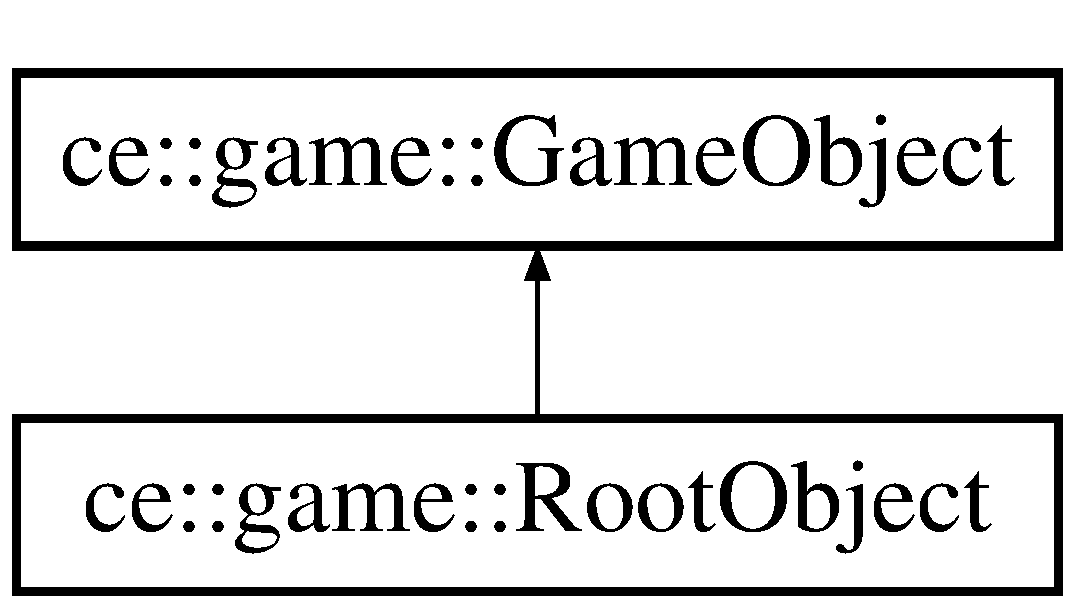
\includegraphics[height=2.000000cm]{classce_1_1game_1_1_root_object}
\end{center}
\end{figure}
\subsection*{Public Member Functions}
\begin{DoxyCompactItemize}
\item 
\mbox{\Hypertarget{classce_1_1game_1_1_root_object_a96e602fe5a016951e643fb06c7a662ce}\label{classce_1_1game_1_1_root_object_a96e602fe5a016951e643fb06c7a662ce}} 
{\bfseries Root\+Object} (\hyperlink{classce_1_1game_1_1_game_object}{Game\+Object} $\ast$parent)=delete
\item 
\mbox{\Hypertarget{classce_1_1game_1_1_root_object_a20e4b6d2b4e0c10fcf8d5141ccb28dfb}\label{classce_1_1game_1_1_root_object_a20e4b6d2b4e0c10fcf8d5141ccb28dfb}} 
{\bfseries Root\+Object} (\hyperlink{classce_1_1game_1_1_game_object}{Game\+Object} $\ast$parent, std\+::string \hyperlink{classce_1_1game_1_1_game_object_a1de1f674c70df3bbba6aefb938ad8f32}{name})=delete
\end{DoxyCompactItemize}
\subsection*{Additional Inherited Members}


The documentation for this class was generated from the following file\+:\begin{DoxyCompactItemize}
\item 
E\+:/\+Development/\+Game\+Engine/\+C\+Engine/src/\+Game/Game\+Object.\+h\end{DoxyCompactItemize}

\hypertarget{classce_1_1game_1_1_scene}{}\section{ce\+:\+:game\+:\+:Scene Class Reference}
\label{classce_1_1game_1_1_scene}\index{ce\+::game\+::\+Scene@{ce\+::game\+::\+Scene}}
\subsection*{Public Member Functions}
\begin{DoxyCompactItemize}
\item 
\mbox{\Hypertarget{classce_1_1game_1_1_scene_af074f86055fe90520e256b7361952485}\label{classce_1_1game_1_1_scene_af074f86055fe90520e256b7361952485}} 
\hyperlink{classce_1_1game_1_1_root_object}{Root\+Object} $\ast$ {\bfseries get\+Root\+Object} ()
\item 
\mbox{\Hypertarget{classce_1_1game_1_1_scene_a86a48ea15dbe591e51741fba1d7860e4}\label{classce_1_1game_1_1_scene_a86a48ea15dbe591e51741fba1d7860e4}} 
\hyperlink{classce_1_1game_1_1_game_object}{Game\+Object} $\ast$ {\bfseries get\+Game\+Object\+By\+Name} (std\+::string name)
\item 
\mbox{\Hypertarget{classce_1_1game_1_1_scene_a77588c7351bc800612fd0ccbcc72c7fc}\label{classce_1_1game_1_1_scene_a77588c7351bc800612fd0ccbcc72c7fc}} 
void {\bfseries init} ()
\item 
\mbox{\Hypertarget{classce_1_1game_1_1_scene_ab39ffabe8aabb8a79f333a1b893ab8c4}\label{classce_1_1game_1_1_scene_ab39ffabe8aabb8a79f333a1b893ab8c4}} 
void {\bfseries begin} ()
\item 
\mbox{\Hypertarget{classce_1_1game_1_1_scene_acddc28540626f6798e1c69dd26fdb1f7}\label{classce_1_1game_1_1_scene_acddc28540626f6798e1c69dd26fdb1f7}} 
void {\bfseries tick} (float dt)
\item 
\mbox{\Hypertarget{classce_1_1game_1_1_scene_a3ad7e4aeeabb3d81bb1aca80453c9e7a}\label{classce_1_1game_1_1_scene_a3ad7e4aeeabb3d81bb1aca80453c9e7a}} 
void {\bfseries draw} (\hyperlink{classce_1_1graphics_1_1_renderer3_d}{ce\+::graphics\+::\+Renderer3D} $\ast$renderer)
\item 
\mbox{\Hypertarget{classce_1_1game_1_1_scene_ac3e467b16eef89bcc2737ccc84b42b3e}\label{classce_1_1game_1_1_scene_ac3e467b16eef89bcc2737ccc84b42b3e}} 
void {\bfseries end} ()
\end{DoxyCompactItemize}


The documentation for this class was generated from the following files\+:\begin{DoxyCompactItemize}
\item 
E\+:/\+Development/\+Game\+Engine/\+C\+Engine/src/\+Game/Scene.\+h\item 
E\+:/\+Development/\+Game\+Engine/\+C\+Engine/src/\+Game/Scene.\+cpp\end{DoxyCompactItemize}

\hypertarget{classce_1_1graphics_1_1_shader}{}\section{ce\+:\+:graphics\+:\+:Shader Class Reference}
\label{classce_1_1graphics_1_1_shader}\index{ce\+::graphics\+::\+Shader@{ce\+::graphics\+::\+Shader}}


\hyperlink{classce_1_1graphics_1_1_shader}{Shader} class mostly a container for the id and contains some helper functions.  




{\ttfamily \#include $<$Shader.\+h$>$}

\subsection*{Public Member Functions}
\begin{DoxyCompactItemize}
\item 
void \hyperlink{classce_1_1graphics_1_1_shader_aca7fefcc416d17e11cf5af7fb36148de}{use} ()
\item 
void \hyperlink{classce_1_1graphics_1_1_shader_a42b65349e86147bbd0fc611eeb4f5890}{set\+Bool} (const std\+::string \&name, bool value) const
\item 
void \hyperlink{classce_1_1graphics_1_1_shader_ab0599b30f759cd140b3c1727673c4665}{set\+Int} (const std\+::string \&name, int value) const
\item 
void \hyperlink{classce_1_1graphics_1_1_shader_a31d56ffb50a079444baf27c863023efc}{set\+Float} (const std\+::string \&name, float value) const
\item 
void \hyperlink{classce_1_1graphics_1_1_shader_a14c07171e23106041bb1dbb683a19d2f}{set\+Vec2} (const std\+::string \&name, const glm\+::vec2 \&value) const
\item 
void \hyperlink{classce_1_1graphics_1_1_shader_aba50173108bd30bcf6f1a4a0446d6a09}{set\+Vec2} (const std\+::string \&name, float x, float y) const
\item 
void \hyperlink{classce_1_1graphics_1_1_shader_ad2ed1ba06e20251009c869e4344605ef}{set\+Vec3} (const std\+::string \&name, const glm\+::vec3 \&value) const
\item 
void \hyperlink{classce_1_1graphics_1_1_shader_aee1a36cd3264b09aed26b99c0fea05ad}{set\+Vec3} (const std\+::string \&name, float x, float y, float z) const
\item 
void \hyperlink{classce_1_1graphics_1_1_shader_a77137819a5a8b7ec1313c19a0aef52b2}{set\+Vec4} (const std\+::string \&name, const glm\+::vec4 \&value) const
\item 
void \hyperlink{classce_1_1graphics_1_1_shader_aa2ce76f7663f91497157017868d4a85e}{set\+Vec4} (const std\+::string \&name, float x, float y, float z, float w) const
\item 
void \hyperlink{classce_1_1graphics_1_1_shader_a6355f9a1480838ce2f1ef8030ef1c259}{set\+Mat2} (const std\+::string \&name, const glm\+::mat2 \&value) const
\item 
void \hyperlink{classce_1_1graphics_1_1_shader_a52a066ab5a24e7f4596931e9c0e325e6}{set\+Mat3} (const std\+::string \&name, const glm\+::mat3 \&value) const
\item 
void \hyperlink{classce_1_1graphics_1_1_shader_ae5f67d260222f5b315ea097b3d898c9f}{set\+Mat4} (const std\+::string \&name, const glm\+::mat4 \&value) const
\end{DoxyCompactItemize}
\subsection*{Protected Attributes}
\begin{DoxyCompactItemize}
\item 
unsigned int \hyperlink{classce_1_1graphics_1_1_shader_a5b5ac3fe6dd6c31fb774d3b670d87c8d}{program\+ID}
\end{DoxyCompactItemize}
\subsection*{Friends}
\begin{DoxyCompactItemize}
\item 
\mbox{\Hypertarget{classce_1_1graphics_1_1_shader_a1ab9ba285584cda12cc4729fccb36f96}\label{classce_1_1graphics_1_1_shader_a1ab9ba285584cda12cc4729fccb36f96}} 
class {\bfseries Shader\+Loader}
\end{DoxyCompactItemize}


\subsection{Detailed Description}
\hyperlink{classce_1_1graphics_1_1_shader}{Shader} class mostly a container for the id and contains some helper functions. 

T\+O\+DO\+: Add geometry shader 

\subsection{Member Function Documentation}
\mbox{\Hypertarget{classce_1_1graphics_1_1_shader_a42b65349e86147bbd0fc611eeb4f5890}\label{classce_1_1graphics_1_1_shader_a42b65349e86147bbd0fc611eeb4f5890}} 
\index{ce\+::graphics\+::\+Shader@{ce\+::graphics\+::\+Shader}!set\+Bool@{set\+Bool}}
\index{set\+Bool@{set\+Bool}!ce\+::graphics\+::\+Shader@{ce\+::graphics\+::\+Shader}}
\subsubsection{\texorpdfstring{set\+Bool()}{setBool()}}
{\footnotesize\ttfamily void ce\+::graphics\+::\+Shader\+::set\+Bool (\begin{DoxyParamCaption}\item[{const std\+::string \&}]{name,  }\item[{bool}]{value }\end{DoxyParamCaption}) const}

Set shader uniform bool \mbox{\Hypertarget{classce_1_1graphics_1_1_shader_a31d56ffb50a079444baf27c863023efc}\label{classce_1_1graphics_1_1_shader_a31d56ffb50a079444baf27c863023efc}} 
\index{ce\+::graphics\+::\+Shader@{ce\+::graphics\+::\+Shader}!set\+Float@{set\+Float}}
\index{set\+Float@{set\+Float}!ce\+::graphics\+::\+Shader@{ce\+::graphics\+::\+Shader}}
\subsubsection{\texorpdfstring{set\+Float()}{setFloat()}}
{\footnotesize\ttfamily void ce\+::graphics\+::\+Shader\+::set\+Float (\begin{DoxyParamCaption}\item[{const std\+::string \&}]{name,  }\item[{float}]{value }\end{DoxyParamCaption}) const}

Set shader uniform float \mbox{\Hypertarget{classce_1_1graphics_1_1_shader_ab0599b30f759cd140b3c1727673c4665}\label{classce_1_1graphics_1_1_shader_ab0599b30f759cd140b3c1727673c4665}} 
\index{ce\+::graphics\+::\+Shader@{ce\+::graphics\+::\+Shader}!set\+Int@{set\+Int}}
\index{set\+Int@{set\+Int}!ce\+::graphics\+::\+Shader@{ce\+::graphics\+::\+Shader}}
\subsubsection{\texorpdfstring{set\+Int()}{setInt()}}
{\footnotesize\ttfamily void ce\+::graphics\+::\+Shader\+::set\+Int (\begin{DoxyParamCaption}\item[{const std\+::string \&}]{name,  }\item[{int}]{value }\end{DoxyParamCaption}) const}

Set shader uniform int \mbox{\Hypertarget{classce_1_1graphics_1_1_shader_a6355f9a1480838ce2f1ef8030ef1c259}\label{classce_1_1graphics_1_1_shader_a6355f9a1480838ce2f1ef8030ef1c259}} 
\index{ce\+::graphics\+::\+Shader@{ce\+::graphics\+::\+Shader}!set\+Mat2@{set\+Mat2}}
\index{set\+Mat2@{set\+Mat2}!ce\+::graphics\+::\+Shader@{ce\+::graphics\+::\+Shader}}
\subsubsection{\texorpdfstring{set\+Mat2()}{setMat2()}}
{\footnotesize\ttfamily void ce\+::graphics\+::\+Shader\+::set\+Mat2 (\begin{DoxyParamCaption}\item[{const std\+::string \&}]{name,  }\item[{const glm\+::mat2 \&}]{value }\end{DoxyParamCaption}) const}

Set shader uniform 2d matrix \mbox{\Hypertarget{classce_1_1graphics_1_1_shader_a52a066ab5a24e7f4596931e9c0e325e6}\label{classce_1_1graphics_1_1_shader_a52a066ab5a24e7f4596931e9c0e325e6}} 
\index{ce\+::graphics\+::\+Shader@{ce\+::graphics\+::\+Shader}!set\+Mat3@{set\+Mat3}}
\index{set\+Mat3@{set\+Mat3}!ce\+::graphics\+::\+Shader@{ce\+::graphics\+::\+Shader}}
\subsubsection{\texorpdfstring{set\+Mat3()}{setMat3()}}
{\footnotesize\ttfamily void ce\+::graphics\+::\+Shader\+::set\+Mat3 (\begin{DoxyParamCaption}\item[{const std\+::string \&}]{name,  }\item[{const glm\+::mat3 \&}]{value }\end{DoxyParamCaption}) const}

Set shader uniform 3d matrix \mbox{\Hypertarget{classce_1_1graphics_1_1_shader_ae5f67d260222f5b315ea097b3d898c9f}\label{classce_1_1graphics_1_1_shader_ae5f67d260222f5b315ea097b3d898c9f}} 
\index{ce\+::graphics\+::\+Shader@{ce\+::graphics\+::\+Shader}!set\+Mat4@{set\+Mat4}}
\index{set\+Mat4@{set\+Mat4}!ce\+::graphics\+::\+Shader@{ce\+::graphics\+::\+Shader}}
\subsubsection{\texorpdfstring{set\+Mat4()}{setMat4()}}
{\footnotesize\ttfamily void ce\+::graphics\+::\+Shader\+::set\+Mat4 (\begin{DoxyParamCaption}\item[{const std\+::string \&}]{name,  }\item[{const glm\+::mat4 \&}]{value }\end{DoxyParamCaption}) const}

Set shader uniform 4d matrix \mbox{\Hypertarget{classce_1_1graphics_1_1_shader_a14c07171e23106041bb1dbb683a19d2f}\label{classce_1_1graphics_1_1_shader_a14c07171e23106041bb1dbb683a19d2f}} 
\index{ce\+::graphics\+::\+Shader@{ce\+::graphics\+::\+Shader}!set\+Vec2@{set\+Vec2}}
\index{set\+Vec2@{set\+Vec2}!ce\+::graphics\+::\+Shader@{ce\+::graphics\+::\+Shader}}
\subsubsection{\texorpdfstring{set\+Vec2()}{setVec2()}\hspace{0.1cm}{\footnotesize\ttfamily [1/2]}}
{\footnotesize\ttfamily void ce\+::graphics\+::\+Shader\+::set\+Vec2 (\begin{DoxyParamCaption}\item[{const std\+::string \&}]{name,  }\item[{const glm\+::vec2 \&}]{value }\end{DoxyParamCaption}) const}

Set shader uniform 2 component vector \mbox{\Hypertarget{classce_1_1graphics_1_1_shader_aba50173108bd30bcf6f1a4a0446d6a09}\label{classce_1_1graphics_1_1_shader_aba50173108bd30bcf6f1a4a0446d6a09}} 
\index{ce\+::graphics\+::\+Shader@{ce\+::graphics\+::\+Shader}!set\+Vec2@{set\+Vec2}}
\index{set\+Vec2@{set\+Vec2}!ce\+::graphics\+::\+Shader@{ce\+::graphics\+::\+Shader}}
\subsubsection{\texorpdfstring{set\+Vec2()}{setVec2()}\hspace{0.1cm}{\footnotesize\ttfamily [2/2]}}
{\footnotesize\ttfamily void ce\+::graphics\+::\+Shader\+::set\+Vec2 (\begin{DoxyParamCaption}\item[{const std\+::string \&}]{name,  }\item[{float}]{x,  }\item[{float}]{y }\end{DoxyParamCaption}) const}

Set shader uniform 2 component vector \mbox{\Hypertarget{classce_1_1graphics_1_1_shader_ad2ed1ba06e20251009c869e4344605ef}\label{classce_1_1graphics_1_1_shader_ad2ed1ba06e20251009c869e4344605ef}} 
\index{ce\+::graphics\+::\+Shader@{ce\+::graphics\+::\+Shader}!set\+Vec3@{set\+Vec3}}
\index{set\+Vec3@{set\+Vec3}!ce\+::graphics\+::\+Shader@{ce\+::graphics\+::\+Shader}}
\subsubsection{\texorpdfstring{set\+Vec3()}{setVec3()}\hspace{0.1cm}{\footnotesize\ttfamily [1/2]}}
{\footnotesize\ttfamily void ce\+::graphics\+::\+Shader\+::set\+Vec3 (\begin{DoxyParamCaption}\item[{const std\+::string \&}]{name,  }\item[{const glm\+::vec3 \&}]{value }\end{DoxyParamCaption}) const}

Set shader uniform 3 component vector \mbox{\Hypertarget{classce_1_1graphics_1_1_shader_aee1a36cd3264b09aed26b99c0fea05ad}\label{classce_1_1graphics_1_1_shader_aee1a36cd3264b09aed26b99c0fea05ad}} 
\index{ce\+::graphics\+::\+Shader@{ce\+::graphics\+::\+Shader}!set\+Vec3@{set\+Vec3}}
\index{set\+Vec3@{set\+Vec3}!ce\+::graphics\+::\+Shader@{ce\+::graphics\+::\+Shader}}
\subsubsection{\texorpdfstring{set\+Vec3()}{setVec3()}\hspace{0.1cm}{\footnotesize\ttfamily [2/2]}}
{\footnotesize\ttfamily void ce\+::graphics\+::\+Shader\+::set\+Vec3 (\begin{DoxyParamCaption}\item[{const std\+::string \&}]{name,  }\item[{float}]{x,  }\item[{float}]{y,  }\item[{float}]{z }\end{DoxyParamCaption}) const}

Set shader uniform 3 component vector \mbox{\Hypertarget{classce_1_1graphics_1_1_shader_a77137819a5a8b7ec1313c19a0aef52b2}\label{classce_1_1graphics_1_1_shader_a77137819a5a8b7ec1313c19a0aef52b2}} 
\index{ce\+::graphics\+::\+Shader@{ce\+::graphics\+::\+Shader}!set\+Vec4@{set\+Vec4}}
\index{set\+Vec4@{set\+Vec4}!ce\+::graphics\+::\+Shader@{ce\+::graphics\+::\+Shader}}
\subsubsection{\texorpdfstring{set\+Vec4()}{setVec4()}\hspace{0.1cm}{\footnotesize\ttfamily [1/2]}}
{\footnotesize\ttfamily void ce\+::graphics\+::\+Shader\+::set\+Vec4 (\begin{DoxyParamCaption}\item[{const std\+::string \&}]{name,  }\item[{const glm\+::vec4 \&}]{value }\end{DoxyParamCaption}) const}

Set shader uniform 4 component vector \mbox{\Hypertarget{classce_1_1graphics_1_1_shader_aa2ce76f7663f91497157017868d4a85e}\label{classce_1_1graphics_1_1_shader_aa2ce76f7663f91497157017868d4a85e}} 
\index{ce\+::graphics\+::\+Shader@{ce\+::graphics\+::\+Shader}!set\+Vec4@{set\+Vec4}}
\index{set\+Vec4@{set\+Vec4}!ce\+::graphics\+::\+Shader@{ce\+::graphics\+::\+Shader}}
\subsubsection{\texorpdfstring{set\+Vec4()}{setVec4()}\hspace{0.1cm}{\footnotesize\ttfamily [2/2]}}
{\footnotesize\ttfamily void ce\+::graphics\+::\+Shader\+::set\+Vec4 (\begin{DoxyParamCaption}\item[{const std\+::string \&}]{name,  }\item[{float}]{x,  }\item[{float}]{y,  }\item[{float}]{z,  }\item[{float}]{w }\end{DoxyParamCaption}) const}

Set shader uniform 4 component vector \mbox{\Hypertarget{classce_1_1graphics_1_1_shader_aca7fefcc416d17e11cf5af7fb36148de}\label{classce_1_1graphics_1_1_shader_aca7fefcc416d17e11cf5af7fb36148de}} 
\index{ce\+::graphics\+::\+Shader@{ce\+::graphics\+::\+Shader}!use@{use}}
\index{use@{use}!ce\+::graphics\+::\+Shader@{ce\+::graphics\+::\+Shader}}
\subsubsection{\texorpdfstring{use()}{use()}}
{\footnotesize\ttfamily void ce\+::graphics\+::\+Shader\+::use (\begin{DoxyParamCaption}{ }\end{DoxyParamCaption})}

Use this shader program 

\subsection{Member Data Documentation}
\mbox{\Hypertarget{classce_1_1graphics_1_1_shader_a5b5ac3fe6dd6c31fb774d3b670d87c8d}\label{classce_1_1graphics_1_1_shader_a5b5ac3fe6dd6c31fb774d3b670d87c8d}} 
\index{ce\+::graphics\+::\+Shader@{ce\+::graphics\+::\+Shader}!program\+ID@{program\+ID}}
\index{program\+ID@{program\+ID}!ce\+::graphics\+::\+Shader@{ce\+::graphics\+::\+Shader}}
\subsubsection{\texorpdfstring{program\+ID}{programID}}
{\footnotesize\ttfamily unsigned int ce\+::graphics\+::\+Shader\+::program\+ID\hspace{0.3cm}{\ttfamily [protected]}}

Open\+GL shader program ID 

The documentation for this class was generated from the following files\+:\begin{DoxyCompactItemize}
\item 
E\+:/\+Development/\+Game\+Engine/\+C\+Engine/src/\+Graphics/\+Shader/\hyperlink{_shader_8h}{Shader.\+h}\item 
E\+:/\+Development/\+Game\+Engine/\+C\+Engine/src/\+Graphics/\+Shader/Shader.\+cpp\end{DoxyCompactItemize}

\hypertarget{classce_1_1graphics_1_1_shader_loader}{}\section{ce\+:\+:graphics\+:\+:Shader\+Loader Class Reference}
\label{classce_1_1graphics_1_1_shader_loader}\index{ce\+::graphics\+::\+Shader\+Loader@{ce\+::graphics\+::\+Shader\+Loader}}


Class used to load shaders.  




{\ttfamily \#include $<$Shader\+Loader.\+h$>$}

\subsection*{Public Member Functions}
\begin{DoxyCompactItemize}
\item 
\hyperlink{classce_1_1graphics_1_1_shader}{Shader} $\ast$ \hyperlink{classce_1_1graphics_1_1_shader_loader_a18279dc40df8efffce0b3d5227bd6af1}{load\+Shader} (\hyperlink{structce_1_1graphics_1_1_shader_properties}{Shader\+Properties} properties)
\item 
bool \hyperlink{classce_1_1graphics_1_1_shader_loader_ae01c71a34d77e36b5aafc142214c6595}{already\+Exists} (\hyperlink{structce_1_1graphics_1_1_shader_properties}{Shader\+Properties} properties)
\end{DoxyCompactItemize}
\subsection*{Protected Member Functions}
\begin{DoxyCompactItemize}
\item 
\hyperlink{classce_1_1graphics_1_1_shader}{Shader} \hyperlink{classce_1_1graphics_1_1_shader_loader_a310a1f7e9478516bc85d03c4a08e6b21}{load\+From\+Source} (const G\+Lchar $\ast$vertex\+Source, const G\+Lchar $\ast$fragment\+Source, const G\+Lchar $\ast$geometry\+Source=\char`\"{}\char`\"{})
\begin{DoxyCompactList}\small\item\em compiles shader code into a program and returns the shader \end{DoxyCompactList}\end{DoxyCompactItemize}


\subsection{Detailed Description}
Class used to load shaders. 

Together with shader properties we make sure we only ever load a shader with the same properties once. 

\subsection{Member Function Documentation}
\mbox{\Hypertarget{classce_1_1graphics_1_1_shader_loader_ae01c71a34d77e36b5aafc142214c6595}\label{classce_1_1graphics_1_1_shader_loader_ae01c71a34d77e36b5aafc142214c6595}} 
\index{ce\+::graphics\+::\+Shader\+Loader@{ce\+::graphics\+::\+Shader\+Loader}!already\+Exists@{already\+Exists}}
\index{already\+Exists@{already\+Exists}!ce\+::graphics\+::\+Shader\+Loader@{ce\+::graphics\+::\+Shader\+Loader}}
\subsubsection{\texorpdfstring{already\+Exists()}{alreadyExists()}}
{\footnotesize\ttfamily bool ce\+::graphics\+::\+Shader\+Loader\+::already\+Exists (\begin{DoxyParamCaption}\item[{\hyperlink{structce_1_1graphics_1_1_shader_properties}{Shader\+Properties}}]{properties }\end{DoxyParamCaption})}

Check if a shader with \hyperlink{structce_1_1graphics_1_1_shader_properties}{Shader\+Properties} has been loaded previously


\begin{DoxyParams}{Parameters}
{\em properties} & \hyperlink{structce_1_1graphics_1_1_shader_properties}{Shader\+Properties} describing the shader \\
\hline
\end{DoxyParams}
\begin{DoxyReturn}{Returns}
True if it has been loaded, false if not 
\end{DoxyReturn}
\mbox{\Hypertarget{classce_1_1graphics_1_1_shader_loader_a310a1f7e9478516bc85d03c4a08e6b21}\label{classce_1_1graphics_1_1_shader_loader_a310a1f7e9478516bc85d03c4a08e6b21}} 
\index{ce\+::graphics\+::\+Shader\+Loader@{ce\+::graphics\+::\+Shader\+Loader}!load\+From\+Source@{load\+From\+Source}}
\index{load\+From\+Source@{load\+From\+Source}!ce\+::graphics\+::\+Shader\+Loader@{ce\+::graphics\+::\+Shader\+Loader}}
\subsubsection{\texorpdfstring{load\+From\+Source()}{loadFromSource()}}
{\footnotesize\ttfamily \hyperlink{classce_1_1graphics_1_1_shader}{ce\+::graphics\+::\+Shader} ce\+::graphics\+::\+Shader\+Loader\+::load\+From\+Source (\begin{DoxyParamCaption}\item[{const G\+Lchar $\ast$}]{vertex\+Source,  }\item[{const G\+Lchar $\ast$}]{fragment\+Source,  }\item[{const G\+Lchar $\ast$}]{geometry\+Source = {\ttfamily \char`\"{}\char`\"{}} }\end{DoxyParamCaption})\hspace{0.3cm}{\ttfamily [protected]}}



compiles shader code into a program and returns the shader 


\begin{DoxyParams}{Parameters}
{\em vertex\+Source} & The source code for the vertex shader \\
\hline
{\em fragment\+Source} & The source code for the fragment shader \\
\hline
{\em geometry\+Source} & The source code for the geometry shader (Yet to be implemented) \\
\hline
\end{DoxyParams}
\begin{DoxyReturn}{Returns}
\hyperlink{classce_1_1graphics_1_1_shader}{Shader} program object. 
\end{DoxyReturn}
\mbox{\Hypertarget{classce_1_1graphics_1_1_shader_loader_a18279dc40df8efffce0b3d5227bd6af1}\label{classce_1_1graphics_1_1_shader_loader_a18279dc40df8efffce0b3d5227bd6af1}} 
\index{ce\+::graphics\+::\+Shader\+Loader@{ce\+::graphics\+::\+Shader\+Loader}!load\+Shader@{load\+Shader}}
\index{load\+Shader@{load\+Shader}!ce\+::graphics\+::\+Shader\+Loader@{ce\+::graphics\+::\+Shader\+Loader}}
\subsubsection{\texorpdfstring{load\+Shader()}{loadShader()}}
{\footnotesize\ttfamily \hyperlink{classce_1_1graphics_1_1_shader}{ce\+::graphics\+::\+Shader} $\ast$ ce\+::graphics\+::\+Shader\+Loader\+::load\+Shader (\begin{DoxyParamCaption}\item[{\hyperlink{structce_1_1graphics_1_1_shader_properties}{Shader\+Properties}}]{properties }\end{DoxyParamCaption})}

Load shader with shader properties


\begin{DoxyParams}{Parameters}
{\em properties} & \hyperlink{structce_1_1graphics_1_1_shader_properties}{Shader\+Properties} describing the shader \\
\hline
\end{DoxyParams}
\begin{DoxyReturn}{Returns}
Pointer to shader program object 
\end{DoxyReturn}


The documentation for this class was generated from the following files\+:\begin{DoxyCompactItemize}
\item 
E\+:/\+Development/\+Game\+Engine/\+C\+Engine/src/\+Graphics/\+Shader/\hyperlink{_shader_loader_8h}{Shader\+Loader.\+h}\item 
E\+:/\+Development/\+Game\+Engine/\+C\+Engine/src/\+Graphics/\+Shader/Shader\+Loader.\+cpp\end{DoxyCompactItemize}

\hypertarget{structce_1_1graphics_1_1_shader_properties}{}\section{ce\+:\+:graphics\+:\+:Shader\+Properties Struct Reference}
\label{structce_1_1graphics_1_1_shader_properties}\index{ce\+::graphics\+::\+Shader\+Properties@{ce\+::graphics\+::\+Shader\+Properties}}


Shader\+Property structure describing what a shader should contain.  




{\ttfamily \#include $<$Shader\+Loader.\+h$>$}

\subsection*{Public Member Functions}
\begin{DoxyCompactItemize}
\item 
bool \hyperlink{structce_1_1graphics_1_1_shader_properties_a36dd41572daba1bed598dee9fbc24cdb}{operator==} (const \hyperlink{structce_1_1graphics_1_1_shader_properties}{Shader\+Properties} \&other) const
\end{DoxyCompactItemize}
\subsection*{Public Attributes}
\begin{DoxyCompactItemize}
\item 
std\+::string \hyperlink{structce_1_1graphics_1_1_shader_properties_a7c292a15c7a6d732c23a859448fadef9}{v\+Path} = \char`\"{}\char`\"{}
\item 
std\+::string \hyperlink{structce_1_1graphics_1_1_shader_properties_a38bb1cbff534647f4e2317e6b00ff14f}{f\+Path} = \char`\"{}\char`\"{}
\item 
std\+::string \hyperlink{structce_1_1graphics_1_1_shader_properties_af1c3a63df0b9520a9cbb00022a5cf32a}{g\+Path} = \char`\"{}\char`\"{}
\item 
unsigned int \hyperlink{structce_1_1graphics_1_1_shader_properties_a7d54a6b908a22b03048b931c68bb1b73}{num\+Dir\+Lights} = 0
\item 
unsigned int \hyperlink{structce_1_1graphics_1_1_shader_properties_a67afcd1acec57748e14ed1ee9705f2bf}{num\+Point\+Lights} = 0
\item 
unsigned int \hyperlink{structce_1_1graphics_1_1_shader_properties_a2345e569f945babf05778559f639eac4}{num\+Spot\+Lights} = 0
\end{DoxyCompactItemize}


\subsection{Detailed Description}
Shader\+Property structure describing what a shader should contain. 

\subsection{Member Function Documentation}
\mbox{\Hypertarget{structce_1_1graphics_1_1_shader_properties_a36dd41572daba1bed598dee9fbc24cdb}\label{structce_1_1graphics_1_1_shader_properties_a36dd41572daba1bed598dee9fbc24cdb}} 
\index{ce\+::graphics\+::\+Shader\+Properties@{ce\+::graphics\+::\+Shader\+Properties}!operator==@{operator==}}
\index{operator==@{operator==}!ce\+::graphics\+::\+Shader\+Properties@{ce\+::graphics\+::\+Shader\+Properties}}
\subsubsection{\texorpdfstring{operator==()}{operator==()}}
{\footnotesize\ttfamily bool ce\+::graphics\+::\+Shader\+Properties\+::operator== (\begin{DoxyParamCaption}\item[{const \hyperlink{structce_1_1graphics_1_1_shader_properties}{Shader\+Properties} \&}]{other }\end{DoxyParamCaption}) const\hspace{0.3cm}{\ttfamily [inline]}}

Comparison operator definition 

\subsection{Member Data Documentation}
\mbox{\Hypertarget{structce_1_1graphics_1_1_shader_properties_a38bb1cbff534647f4e2317e6b00ff14f}\label{structce_1_1graphics_1_1_shader_properties_a38bb1cbff534647f4e2317e6b00ff14f}} 
\index{ce\+::graphics\+::\+Shader\+Properties@{ce\+::graphics\+::\+Shader\+Properties}!f\+Path@{f\+Path}}
\index{f\+Path@{f\+Path}!ce\+::graphics\+::\+Shader\+Properties@{ce\+::graphics\+::\+Shader\+Properties}}
\subsubsection{\texorpdfstring{f\+Path}{fPath}}
{\footnotesize\ttfamily std\+::string ce\+::graphics\+::\+Shader\+Properties\+::f\+Path = \char`\"{}\char`\"{}}

Fragment shader path \mbox{\Hypertarget{structce_1_1graphics_1_1_shader_properties_af1c3a63df0b9520a9cbb00022a5cf32a}\label{structce_1_1graphics_1_1_shader_properties_af1c3a63df0b9520a9cbb00022a5cf32a}} 
\index{ce\+::graphics\+::\+Shader\+Properties@{ce\+::graphics\+::\+Shader\+Properties}!g\+Path@{g\+Path}}
\index{g\+Path@{g\+Path}!ce\+::graphics\+::\+Shader\+Properties@{ce\+::graphics\+::\+Shader\+Properties}}
\subsubsection{\texorpdfstring{g\+Path}{gPath}}
{\footnotesize\ttfamily std\+::string ce\+::graphics\+::\+Shader\+Properties\+::g\+Path = \char`\"{}\char`\"{}}

Geometry shader path \mbox{\Hypertarget{structce_1_1graphics_1_1_shader_properties_a7d54a6b908a22b03048b931c68bb1b73}\label{structce_1_1graphics_1_1_shader_properties_a7d54a6b908a22b03048b931c68bb1b73}} 
\index{ce\+::graphics\+::\+Shader\+Properties@{ce\+::graphics\+::\+Shader\+Properties}!num\+Dir\+Lights@{num\+Dir\+Lights}}
\index{num\+Dir\+Lights@{num\+Dir\+Lights}!ce\+::graphics\+::\+Shader\+Properties@{ce\+::graphics\+::\+Shader\+Properties}}
\subsubsection{\texorpdfstring{num\+Dir\+Lights}{numDirLights}}
{\footnotesize\ttfamily unsigned int ce\+::graphics\+::\+Shader\+Properties\+::num\+Dir\+Lights = 0}

Number of directional lights it needs to support \mbox{\Hypertarget{structce_1_1graphics_1_1_shader_properties_a67afcd1acec57748e14ed1ee9705f2bf}\label{structce_1_1graphics_1_1_shader_properties_a67afcd1acec57748e14ed1ee9705f2bf}} 
\index{ce\+::graphics\+::\+Shader\+Properties@{ce\+::graphics\+::\+Shader\+Properties}!num\+Point\+Lights@{num\+Point\+Lights}}
\index{num\+Point\+Lights@{num\+Point\+Lights}!ce\+::graphics\+::\+Shader\+Properties@{ce\+::graphics\+::\+Shader\+Properties}}
\subsubsection{\texorpdfstring{num\+Point\+Lights}{numPointLights}}
{\footnotesize\ttfamily unsigned int ce\+::graphics\+::\+Shader\+Properties\+::num\+Point\+Lights = 0}

Number of point lights it needs to support \mbox{\Hypertarget{structce_1_1graphics_1_1_shader_properties_a2345e569f945babf05778559f639eac4}\label{structce_1_1graphics_1_1_shader_properties_a2345e569f945babf05778559f639eac4}} 
\index{ce\+::graphics\+::\+Shader\+Properties@{ce\+::graphics\+::\+Shader\+Properties}!num\+Spot\+Lights@{num\+Spot\+Lights}}
\index{num\+Spot\+Lights@{num\+Spot\+Lights}!ce\+::graphics\+::\+Shader\+Properties@{ce\+::graphics\+::\+Shader\+Properties}}
\subsubsection{\texorpdfstring{num\+Spot\+Lights}{numSpotLights}}
{\footnotesize\ttfamily unsigned int ce\+::graphics\+::\+Shader\+Properties\+::num\+Spot\+Lights = 0}

Number of spot lights it needs to support \mbox{\Hypertarget{structce_1_1graphics_1_1_shader_properties_a7c292a15c7a6d732c23a859448fadef9}\label{structce_1_1graphics_1_1_shader_properties_a7c292a15c7a6d732c23a859448fadef9}} 
\index{ce\+::graphics\+::\+Shader\+Properties@{ce\+::graphics\+::\+Shader\+Properties}!v\+Path@{v\+Path}}
\index{v\+Path@{v\+Path}!ce\+::graphics\+::\+Shader\+Properties@{ce\+::graphics\+::\+Shader\+Properties}}
\subsubsection{\texorpdfstring{v\+Path}{vPath}}
{\footnotesize\ttfamily std\+::string ce\+::graphics\+::\+Shader\+Properties\+::v\+Path = \char`\"{}\char`\"{}}

\hyperlink{structce_1_1graphics_1_1_vertex}{Vertex} shader path 

The documentation for this struct was generated from the following file\+:\begin{DoxyCompactItemize}
\item 
E\+:/\+Development/\+Game\+Engine/\+C\+Engine/src/\+Graphics/\+Shader/\hyperlink{_shader_loader_8h}{Shader\+Loader.\+h}\end{DoxyCompactItemize}

\hypertarget{classce_1_1graphics_1_1_spot_light}{}\section{ce\+:\+:graphics\+:\+:Spot\+Light Class Reference}
\label{classce_1_1graphics_1_1_spot_light}\index{ce\+::graphics\+::\+Spot\+Light@{ce\+::graphics\+::\+Spot\+Light}}


A spot light.  




{\ttfamily \#include $<$Lights.\+h$>$}

Inheritance diagram for ce\+:\+:graphics\+:\+:Spot\+Light\+:\begin{figure}[H]
\begin{center}
\leavevmode
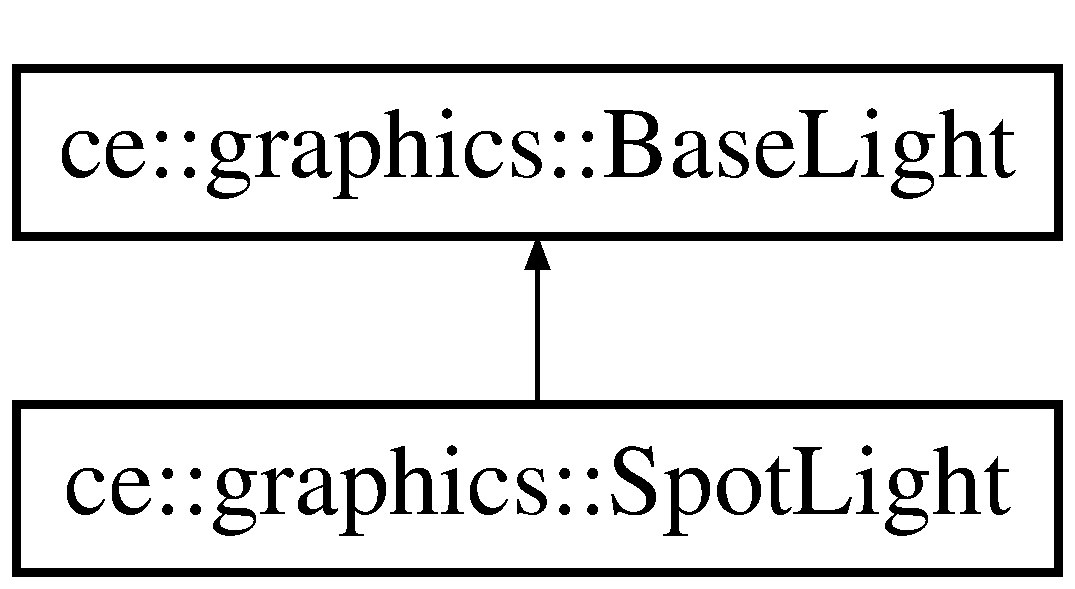
\includegraphics[height=2.000000cm]{classce_1_1graphics_1_1_spot_light}
\end{center}
\end{figure}
\subsection*{Public Attributes}
\begin{DoxyCompactItemize}
\item 
\mbox{\Hypertarget{classce_1_1graphics_1_1_spot_light_a84a6b12c9c9a761d54672d68bcf5e2b0}\label{classce_1_1graphics_1_1_spot_light_a84a6b12c9c9a761d54672d68bcf5e2b0}} 
glm\+::vec3 {\bfseries position} = glm\+::vec3(0.\+0f, 0.\+0f, 0.\+0f)
\item 
\mbox{\Hypertarget{classce_1_1graphics_1_1_spot_light_a18634cf5c779fd34efb3298774f02d24}\label{classce_1_1graphics_1_1_spot_light_a18634cf5c779fd34efb3298774f02d24}} 
glm\+::vec3 {\bfseries direction} = glm\+::vec3(0.\+0f, 0.\+0f, 1.\+0f)
\item 
\mbox{\Hypertarget{classce_1_1graphics_1_1_spot_light_a6cb09e93a8cc20ba0f6ed21fcfc0f720}\label{classce_1_1graphics_1_1_spot_light_a6cb09e93a8cc20ba0f6ed21fcfc0f720}} 
float {\bfseries constant} = 1.\+0f
\item 
\mbox{\Hypertarget{classce_1_1graphics_1_1_spot_light_af9bd65024e9ee84e0a2aae9dda6a8807}\label{classce_1_1graphics_1_1_spot_light_af9bd65024e9ee84e0a2aae9dda6a8807}} 
float {\bfseries linear} = 0.\+09f
\item 
\mbox{\Hypertarget{classce_1_1graphics_1_1_spot_light_a6afbb4be9fda216b86dfba608aa4c2dd}\label{classce_1_1graphics_1_1_spot_light_a6afbb4be9fda216b86dfba608aa4c2dd}} 
float {\bfseries quadratic} = 0.\+032f
\item 
\mbox{\Hypertarget{classce_1_1graphics_1_1_spot_light_af4b4eac01e5396be4a95fdf09e86363c}\label{classce_1_1graphics_1_1_spot_light_af4b4eac01e5396be4a95fdf09e86363c}} 
float {\bfseries cut\+Off} = 0.\+96f
\item 
\mbox{\Hypertarget{classce_1_1graphics_1_1_spot_light_a0cb85ec1332296f31b744b5aaa326c1b}\label{classce_1_1graphics_1_1_spot_light_a0cb85ec1332296f31b744b5aaa326c1b}} 
float {\bfseries outer\+Cut\+Off} = 0.\+90f
\end{DoxyCompactItemize}


\subsection{Detailed Description}
A spot light. 

The documentation for this class was generated from the following file\+:\begin{DoxyCompactItemize}
\item 
Graphics/\hyperlink{_lights_8h}{Lights.\+h}\end{DoxyCompactItemize}

\hypertarget{classce_1_1graphics_1_1_text}{}\section{ce\+:\+:graphics\+:\+:Text Class Reference}
\label{classce_1_1graphics_1_1_text}\index{ce\+::graphics\+::\+Text@{ce\+::graphics\+::\+Text}}


A renderable piece of text.  




{\ttfamily \#include $<$Text.\+h$>$}

\subsection*{Public Member Functions}
\begin{DoxyCompactItemize}
\item 
\mbox{\Hypertarget{classce_1_1graphics_1_1_text_a54e3ef845a5ae19f298f84c768280fb2}\label{classce_1_1graphics_1_1_text_a54e3ef845a5ae19f298f84c768280fb2}} 
void {\bfseries set\+Font} (\hyperlink{classce_1_1graphics_1_1_font}{Font} $\ast$font)
\item 
\mbox{\Hypertarget{classce_1_1graphics_1_1_text_a6d91d8e541393513dc999cb9f7627ee5}\label{classce_1_1graphics_1_1_text_a6d91d8e541393513dc999cb9f7627ee5}} 
void {\bfseries set\+Text} (std\+::string text)
\item 
\mbox{\Hypertarget{classce_1_1graphics_1_1_text_a7f3a666a2a6a0725a61c1cecc437d832}\label{classce_1_1graphics_1_1_text_a7f3a666a2a6a0725a61c1cecc437d832}} 
void {\bfseries set\+Size} (unsigned int size)
\item 
\mbox{\Hypertarget{classce_1_1graphics_1_1_text_ac9757fb654ae91f3c80eb04f1e7422f9}\label{classce_1_1graphics_1_1_text_ac9757fb654ae91f3c80eb04f1e7422f9}} 
void {\bfseries set\+Position} (int x, int y)
\item 
\mbox{\Hypertarget{classce_1_1graphics_1_1_text_a97ceb3ee07e53939d0de53546147ef21}\label{classce_1_1graphics_1_1_text_a97ceb3ee07e53939d0de53546147ef21}} 
void {\bfseries set\+Position} (glm\+::ivec2 pos)
\item 
\mbox{\Hypertarget{classce_1_1graphics_1_1_text_a65b3eeebadc7b36bffe6abc5fcaf7256}\label{classce_1_1graphics_1_1_text_a65b3eeebadc7b36bffe6abc5fcaf7256}} 
void {\bfseries set\+Color} (glm\+::vec4 color)
\item 
\mbox{\Hypertarget{classce_1_1graphics_1_1_text_a4a88235e0f0a7c5e3b5c529f637a1d49}\label{classce_1_1graphics_1_1_text_a4a88235e0f0a7c5e3b5c529f637a1d49}} 
void {\bfseries set\+Color} (float r, float g, float b, float a=1.\+0f)
\item 
\mbox{\Hypertarget{classce_1_1graphics_1_1_text_a069d0ec7f8f03fc12228d1fb1f407f27}\label{classce_1_1graphics_1_1_text_a069d0ec7f8f03fc12228d1fb1f407f27}} 
void {\bfseries draw} (\hyperlink{classce_1_1graphics_1_1_shader}{ce\+::graphics\+::\+Shader} shader)
\item 
\mbox{\Hypertarget{classce_1_1graphics_1_1_text_ac7e5b5679947244d96cc4d592d364936}\label{classce_1_1graphics_1_1_text_ac7e5b5679947244d96cc4d592d364936}} 
std\+::string {\bfseries get\+Text} ()
\end{DoxyCompactItemize}
\subsection*{Protected Member Functions}
\begin{DoxyCompactItemize}
\item 
void \hyperlink{classce_1_1graphics_1_1_text_a666aae08c7a6c6344b0722ffbefd6fb3}{update} ()
\end{DoxyCompactItemize}
\subsection*{Protected Attributes}
\begin{DoxyCompactItemize}
\item 
\mbox{\Hypertarget{classce_1_1graphics_1_1_text_ac24aa6948fcd48f365e8327dc0b0db73}\label{classce_1_1graphics_1_1_text_ac24aa6948fcd48f365e8327dc0b0db73}} 
\hyperlink{classce_1_1graphics_1_1_font}{ce\+::graphics\+::\+Font} $\ast$ {\bfseries m\+\_\+font}
\item 
\mbox{\Hypertarget{classce_1_1graphics_1_1_text_a172659977452467ed56f00182ba67c13}\label{classce_1_1graphics_1_1_text_a172659977452467ed56f00182ba67c13}} 
std\+::string {\bfseries m\+\_\+text} = \char`\"{}\char`\"{}
\item 
\mbox{\Hypertarget{classce_1_1graphics_1_1_text_a4f11e340917dbd28cb664a96d8d63ae5}\label{classce_1_1graphics_1_1_text_a4f11e340917dbd28cb664a96d8d63ae5}} 
unsigned int {\bfseries m\+\_\+size} = 48
\item 
\mbox{\Hypertarget{classce_1_1graphics_1_1_text_a6a154160a60e196464a2371df2a5cf72}\label{classce_1_1graphics_1_1_text_a6a154160a60e196464a2371df2a5cf72}} 
glm\+::ivec2 {\bfseries m\+\_\+position}
\item 
\mbox{\Hypertarget{classce_1_1graphics_1_1_text_ae23869942fc68b6e59131574fb0aa7a7}\label{classce_1_1graphics_1_1_text_ae23869942fc68b6e59131574fb0aa7a7}} 
glm\+::vec4 {\bfseries m\+\_\+color} = glm\+::vec4(1.\+0f, 1.\+0f, 1.\+0f, 1.\+0f)
\item 
\mbox{\Hypertarget{classce_1_1graphics_1_1_text_a3290f89985cc8b4f74051235f281d157}\label{classce_1_1graphics_1_1_text_a3290f89985cc8b4f74051235f281d157}} 
std\+::vector$<$ \hyperlink{structce_1_1graphics_1_1_character}{ce\+::graphics\+::\+Character} $>$ {\bfseries m\+\_\+characters}
\item 
\mbox{\Hypertarget{classce_1_1graphics_1_1_text_a152e95edbed3733f77d6036985e918f6}\label{classce_1_1graphics_1_1_text_a152e95edbed3733f77d6036985e918f6}} 
G\+Luint {\bfseries m\+\_\+\+V\+AO}
\item 
\mbox{\Hypertarget{classce_1_1graphics_1_1_text_a7e5a825933c15cf45ce80de33eb941b7}\label{classce_1_1graphics_1_1_text_a7e5a825933c15cf45ce80de33eb941b7}} 
G\+Luint {\bfseries m\+\_\+\+V\+BO}
\end{DoxyCompactItemize}


\subsection{Detailed Description}
A renderable piece of text. 

\subsection{Member Function Documentation}
\mbox{\Hypertarget{classce_1_1graphics_1_1_text_a666aae08c7a6c6344b0722ffbefd6fb3}\label{classce_1_1graphics_1_1_text_a666aae08c7a6c6344b0722ffbefd6fb3}} 
\index{ce\+::graphics\+::\+Text@{ce\+::graphics\+::\+Text}!update@{update}}
\index{update@{update}!ce\+::graphics\+::\+Text@{ce\+::graphics\+::\+Text}}
\subsubsection{\texorpdfstring{update()}{update()}}
{\footnotesize\ttfamily void ce\+::graphics\+::\+Text\+::update (\begin{DoxyParamCaption}{ }\end{DoxyParamCaption})\hspace{0.3cm}{\ttfamily [protected]}}

Updates the characters 

The documentation for this class was generated from the following files\+:\begin{DoxyCompactItemize}
\item 
E\+:/\+Development/\+Game\+Engine/\+C\+Engine/src/\+Graphics/\+Text/Text.\+h\item 
E\+:/\+Development/\+Game\+Engine/\+C\+Engine/src/\+Graphics/\+Text/Text.\+cpp\end{DoxyCompactItemize}

\hypertarget{structce_1_1graphics_1_1_texture}{}\section{ce\+:\+:graphics\+:\+:Texture Struct Reference}
\label{structce_1_1graphics_1_1_texture}\index{ce\+::graphics\+::\+Texture@{ce\+::graphics\+::\+Texture}}


A structure describing a texture.  




{\ttfamily \#include $<$Texture.\+h$>$}

\subsection*{Public Attributes}
\begin{DoxyCompactItemize}
\item 
unsigned int \hyperlink{structce_1_1graphics_1_1_texture_af9e415b9175764428d5d6dddd1778e93}{id}
\item 
\hyperlink{_texture_8h_aefaa1df613346ad1fea779bc9a04fdd7}{Texture\+Type} \hyperlink{structce_1_1graphics_1_1_texture_a0c6ddb1eacae739d37e336ea03fa01ec}{type}
\end{DoxyCompactItemize}


\subsection{Detailed Description}
A structure describing a texture. 

\subsection{Member Data Documentation}
\mbox{\Hypertarget{structce_1_1graphics_1_1_texture_af9e415b9175764428d5d6dddd1778e93}\label{structce_1_1graphics_1_1_texture_af9e415b9175764428d5d6dddd1778e93}} 
\index{ce\+::graphics\+::\+Texture@{ce\+::graphics\+::\+Texture}!id@{id}}
\index{id@{id}!ce\+::graphics\+::\+Texture@{ce\+::graphics\+::\+Texture}}
\subsubsection{\texorpdfstring{id}{id}}
{\footnotesize\ttfamily unsigned int ce\+::graphics\+::\+Texture\+::id}

\hyperlink{structce_1_1graphics_1_1_texture}{Texture} id internally of Open\+GL \mbox{\Hypertarget{structce_1_1graphics_1_1_texture_a0c6ddb1eacae739d37e336ea03fa01ec}\label{structce_1_1graphics_1_1_texture_a0c6ddb1eacae739d37e336ea03fa01ec}} 
\index{ce\+::graphics\+::\+Texture@{ce\+::graphics\+::\+Texture}!type@{type}}
\index{type@{type}!ce\+::graphics\+::\+Texture@{ce\+::graphics\+::\+Texture}}
\subsubsection{\texorpdfstring{type}{type}}
{\footnotesize\ttfamily \hyperlink{_texture_8h_aefaa1df613346ad1fea779bc9a04fdd7}{Texture\+Type} ce\+::graphics\+::\+Texture\+::type}

The texture type used to determine what kind of texture this is 

The documentation for this struct was generated from the following file\+:\begin{DoxyCompactItemize}
\item 
E\+:/\+Development/\+Game\+Engine/\+C\+Engine/src/\+Graphics/\hyperlink{_texture_8h}{Texture.\+h}\end{DoxyCompactItemize}

\hypertarget{structce_1_1core_1_1_time}{}\section{ce\+:\+:core\+:\+:Time Struct Reference}
\label{structce_1_1core_1_1_time}\index{ce\+::core\+::\+Time@{ce\+::core\+::\+Time}}


Represents time in diffrent formats.  




{\ttfamily \#include $<$Time.\+h$>$}

\subsection*{Public Member Functions}
\begin{DoxyCompactItemize}
\item 
\mbox{\Hypertarget{structce_1_1core_1_1_time_aa418056d22ac6c29edfb05a5bba319ec}\label{structce_1_1core_1_1_time_aa418056d22ac6c29edfb05a5bba319ec}} 
int {\bfseries as\+Microseconds} ()
\item 
\mbox{\Hypertarget{structce_1_1core_1_1_time_a7e4e98c781cc94efff0092fcf373b067}\label{structce_1_1core_1_1_time_a7e4e98c781cc94efff0092fcf373b067}} 
int {\bfseries as\+Milliseconds} ()
\item 
\mbox{\Hypertarget{structce_1_1core_1_1_time_a2d55e757931da557abf5ec8a73404f47}\label{structce_1_1core_1_1_time_a2d55e757931da557abf5ec8a73404f47}} 
float {\bfseries as\+Seconds} ()
\end{DoxyCompactItemize}
\subsection*{Public Attributes}
\begin{DoxyCompactItemize}
\item 
int \hyperlink{structce_1_1core_1_1_time_a9c46ccd85022eb7a5374b2a28cfc9c97}{time} = 0
\end{DoxyCompactItemize}


\subsection{Detailed Description}
Represents time in diffrent formats. 

Internally uses milliseconds and easily transfers it to other formats for use in the engine. 

\subsection{Member Data Documentation}
\mbox{\Hypertarget{structce_1_1core_1_1_time_a9c46ccd85022eb7a5374b2a28cfc9c97}\label{structce_1_1core_1_1_time_a9c46ccd85022eb7a5374b2a28cfc9c97}} 
\index{ce\+::core\+::\+Time@{ce\+::core\+::\+Time}!time@{time}}
\index{time@{time}!ce\+::core\+::\+Time@{ce\+::core\+::\+Time}}
\subsubsection{\texorpdfstring{time}{time}}
{\footnotesize\ttfamily int ce\+::core\+::\+Time\+::time = 0}

The time in milliseconds 

The documentation for this struct was generated from the following file\+:\begin{DoxyCompactItemize}
\item 
Core/Time.\+h\end{DoxyCompactItemize}

\hypertarget{classce_1_1graphics_1_1_transform}{}\section{ce\+:\+:graphics\+:\+:Transform Class Reference}
\label{classce_1_1graphics_1_1_transform}\index{ce\+::graphics\+::\+Transform@{ce\+::graphics\+::\+Transform}}
Inheritance diagram for ce\+:\+:graphics\+:\+:Transform\+:\begin{figure}[H]
\begin{center}
\leavevmode
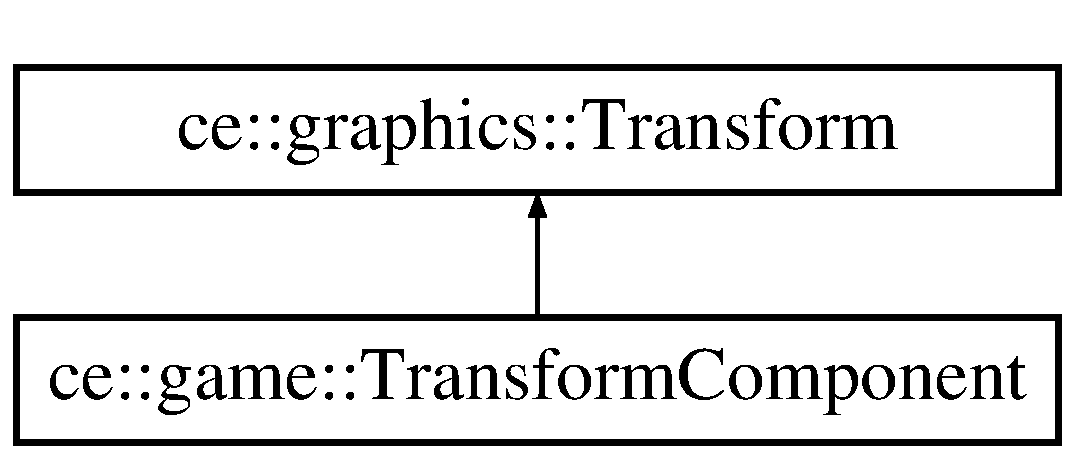
\includegraphics[height=2.000000cm]{classce_1_1graphics_1_1_transform}
\end{center}
\end{figure}
\subsection*{Public Member Functions}
\begin{DoxyCompactItemize}
\item 
\mbox{\Hypertarget{classce_1_1graphics_1_1_transform_a8a20d37b8a97e44d194ee295110b9b45}\label{classce_1_1graphics_1_1_transform_a8a20d37b8a97e44d194ee295110b9b45}} 
glm\+::mat4 {\bfseries get\+As\+Matrix} ()
\item 
\mbox{\Hypertarget{classce_1_1graphics_1_1_transform_ad7884dbbcc4d83d08f22f5c36027b7b6}\label{classce_1_1graphics_1_1_transform_ad7884dbbcc4d83d08f22f5c36027b7b6}} 
void {\bfseries pitch} (float degrees)
\item 
\mbox{\Hypertarget{classce_1_1graphics_1_1_transform_abf69da0f56c81e8839d73e4642fb25ae}\label{classce_1_1graphics_1_1_transform_abf69da0f56c81e8839d73e4642fb25ae}} 
void {\bfseries yaw} (float degrees)
\item 
\mbox{\Hypertarget{classce_1_1graphics_1_1_transform_a6887f9680002a61d62b14fa4a5582352}\label{classce_1_1graphics_1_1_transform_a6887f9680002a61d62b14fa4a5582352}} 
void {\bfseries roll} (float degrees)
\item 
\mbox{\Hypertarget{classce_1_1graphics_1_1_transform_a118c8fc699bfb8e4326cd73ac8cb7e6b}\label{classce_1_1graphics_1_1_transform_a118c8fc699bfb8e4326cd73ac8cb7e6b}} 
void {\bfseries rotate} (float x, float y, float z)
\item 
\mbox{\Hypertarget{classce_1_1graphics_1_1_transform_a9afc18fc3eb7b81c34b754f146ddbea1}\label{classce_1_1graphics_1_1_transform_a9afc18fc3eb7b81c34b754f146ddbea1}} 
void {\bfseries rotate} (glm\+::vec3 degrees)
\item 
\mbox{\Hypertarget{classce_1_1graphics_1_1_transform_af31b6c66a88f5094b96f52d114207f85}\label{classce_1_1graphics_1_1_transform_af31b6c66a88f5094b96f52d114207f85}} 
void {\bfseries set\+Rotation} (float x, float y, float z)
\item 
\mbox{\Hypertarget{classce_1_1graphics_1_1_transform_a1d487f86fde7aebea571e0ab43598426}\label{classce_1_1graphics_1_1_transform_a1d487f86fde7aebea571e0ab43598426}} 
void {\bfseries set\+Rotation} (glm\+::vec3 degrees)
\item 
\mbox{\Hypertarget{classce_1_1graphics_1_1_transform_a129359a6fb87eccff8a9c120e68ba70d}\label{classce_1_1graphics_1_1_transform_a129359a6fb87eccff8a9c120e68ba70d}} 
glm\+::vec3 {\bfseries get\+Rotation} ()
\item 
\mbox{\Hypertarget{classce_1_1graphics_1_1_transform_a58a28b5d5e04159982de7fb8918f22e0}\label{classce_1_1graphics_1_1_transform_a58a28b5d5e04159982de7fb8918f22e0}} 
glm\+::quat {\bfseries get\+Orientation} ()
\item 
void \hyperlink{classce_1_1graphics_1_1_transform_af9eee7c8504d7f2e5e26446fcd24ec30}{translate} (float x, float y, float z)
\item 
void \hyperlink{classce_1_1graphics_1_1_transform_ac9574ab0474bcf721a89f914538a7400}{translate} (glm\+::vec3 xyz)
\item 
\mbox{\Hypertarget{classce_1_1graphics_1_1_transform_a3ddbb100852c1e320e2900ba768683d2}\label{classce_1_1graphics_1_1_transform_a3ddbb100852c1e320e2900ba768683d2}} 
void {\bfseries move} (float x, float y, float z)
\item 
\mbox{\Hypertarget{classce_1_1graphics_1_1_transform_ab762980b651270b25ec8839eab294f1c}\label{classce_1_1graphics_1_1_transform_ab762980b651270b25ec8839eab294f1c}} 
void {\bfseries move} (glm\+::vec3 xyz)
\item 
\mbox{\Hypertarget{classce_1_1graphics_1_1_transform_a4dcb88eaed843b31d6e496dcb6fe19d5}\label{classce_1_1graphics_1_1_transform_a4dcb88eaed843b31d6e496dcb6fe19d5}} 
void {\bfseries set\+Position} (float x, float y, float z)
\item 
\mbox{\Hypertarget{classce_1_1graphics_1_1_transform_ac1f54a03a3e1e6b1b2581890256a26a2}\label{classce_1_1graphics_1_1_transform_ac1f54a03a3e1e6b1b2581890256a26a2}} 
void {\bfseries set\+Position} (glm\+::vec3 xyz)
\item 
\mbox{\Hypertarget{classce_1_1graphics_1_1_transform_a86443441ce2649ca345fb5490a85a1ba}\label{classce_1_1graphics_1_1_transform_a86443441ce2649ca345fb5490a85a1ba}} 
glm\+::vec3 {\bfseries get\+Position} ()
\item 
\mbox{\Hypertarget{classce_1_1graphics_1_1_transform_ac4ba6a9b9f67ab7839ca354102fb5e4d}\label{classce_1_1graphics_1_1_transform_ac4ba6a9b9f67ab7839ca354102fb5e4d}} 
void {\bfseries scale} (float x, float y, float z)
\item 
\mbox{\Hypertarget{classce_1_1graphics_1_1_transform_a496b3fd3935e15ac079233fbd9f76ccd}\label{classce_1_1graphics_1_1_transform_a496b3fd3935e15ac079233fbd9f76ccd}} 
void {\bfseries scale} (glm\+::vec3 xyz)
\item 
\mbox{\Hypertarget{classce_1_1graphics_1_1_transform_a101c16a5b94887a91dad8fe18584f597}\label{classce_1_1graphics_1_1_transform_a101c16a5b94887a91dad8fe18584f597}} 
void {\bfseries set\+Scale} (float x, float y, float z)
\item 
\mbox{\Hypertarget{classce_1_1graphics_1_1_transform_a7524e1a25dbc5b3d940871efd3ebb49f}\label{classce_1_1graphics_1_1_transform_a7524e1a25dbc5b3d940871efd3ebb49f}} 
void {\bfseries set\+Scale} (glm\+::vec3 xyz)
\item 
\mbox{\Hypertarget{classce_1_1graphics_1_1_transform_a1f4d4f46ae6610fc339d4acfbf2590d5}\label{classce_1_1graphics_1_1_transform_a1f4d4f46ae6610fc339d4acfbf2590d5}} 
glm\+::vec3 {\bfseries get\+Scale} ()
\end{DoxyCompactItemize}
\subsection*{Protected Attributes}
\begin{DoxyCompactItemize}
\item 
glm\+::vec3 \hyperlink{classce_1_1graphics_1_1_transform_ac55ab1bffbe1250d4bef77798180d592}{m\+\_\+position}
\begin{DoxyCompactList}\small\item\em Our position vector. \end{DoxyCompactList}\item 
glm\+::vec3 \hyperlink{classce_1_1graphics_1_1_transform_a88394bb0517cf741b97f9c9c76d3775e}{m\+\_\+scale}
\begin{DoxyCompactList}\small\item\em Our scale vector. \end{DoxyCompactList}\item 
glm\+::vec3 \hyperlink{classce_1_1graphics_1_1_transform_a1952fc3789a58ab6bb54887bc8374693}{m\+\_\+rotation}
\end{DoxyCompactItemize}


\subsection{Member Function Documentation}
\mbox{\Hypertarget{classce_1_1graphics_1_1_transform_af9eee7c8504d7f2e5e26446fcd24ec30}\label{classce_1_1graphics_1_1_transform_af9eee7c8504d7f2e5e26446fcd24ec30}} 
\index{ce\+::graphics\+::\+Transform@{ce\+::graphics\+::\+Transform}!translate@{translate}}
\index{translate@{translate}!ce\+::graphics\+::\+Transform@{ce\+::graphics\+::\+Transform}}
\subsubsection{\texorpdfstring{translate()}{translate()}\hspace{0.1cm}{\footnotesize\ttfamily [1/2]}}
{\footnotesize\ttfamily void ce\+::graphics\+::\+Transform\+::translate (\begin{DoxyParamCaption}\item[{float}]{x,  }\item[{float}]{y,  }\item[{float}]{z }\end{DoxyParamCaption})}

Translate relative to orientation \mbox{\Hypertarget{classce_1_1graphics_1_1_transform_ac9574ab0474bcf721a89f914538a7400}\label{classce_1_1graphics_1_1_transform_ac9574ab0474bcf721a89f914538a7400}} 
\index{ce\+::graphics\+::\+Transform@{ce\+::graphics\+::\+Transform}!translate@{translate}}
\index{translate@{translate}!ce\+::graphics\+::\+Transform@{ce\+::graphics\+::\+Transform}}
\subsubsection{\texorpdfstring{translate()}{translate()}\hspace{0.1cm}{\footnotesize\ttfamily [2/2]}}
{\footnotesize\ttfamily void ce\+::graphics\+::\+Transform\+::translate (\begin{DoxyParamCaption}\item[{glm\+::vec3}]{xyz }\end{DoxyParamCaption})}

Translate relative to orientation 

\subsection{Member Data Documentation}
\mbox{\Hypertarget{classce_1_1graphics_1_1_transform_ac55ab1bffbe1250d4bef77798180d592}\label{classce_1_1graphics_1_1_transform_ac55ab1bffbe1250d4bef77798180d592}} 
\index{ce\+::graphics\+::\+Transform@{ce\+::graphics\+::\+Transform}!m\+\_\+position@{m\+\_\+position}}
\index{m\+\_\+position@{m\+\_\+position}!ce\+::graphics\+::\+Transform@{ce\+::graphics\+::\+Transform}}
\subsubsection{\texorpdfstring{m\+\_\+position}{m\_position}}
{\footnotesize\ttfamily glm\+::vec3 ce\+::graphics\+::\+Transform\+::m\+\_\+position\hspace{0.3cm}{\ttfamily [protected]}}



Our position vector. 

Each axis represents the position on said axis \mbox{\Hypertarget{classce_1_1graphics_1_1_transform_a1952fc3789a58ab6bb54887bc8374693}\label{classce_1_1graphics_1_1_transform_a1952fc3789a58ab6bb54887bc8374693}} 
\index{ce\+::graphics\+::\+Transform@{ce\+::graphics\+::\+Transform}!m\+\_\+rotation@{m\+\_\+rotation}}
\index{m\+\_\+rotation@{m\+\_\+rotation}!ce\+::graphics\+::\+Transform@{ce\+::graphics\+::\+Transform}}
\subsubsection{\texorpdfstring{m\+\_\+rotation}{m\_rotation}}
{\footnotesize\ttfamily glm\+::vec3 ce\+::graphics\+::\+Transform\+::m\+\_\+rotation\hspace{0.3cm}{\ttfamily [protected]}}

Our rotation vector in eular angles

Each axis represents the degrees of rotation on said axis \mbox{\Hypertarget{classce_1_1graphics_1_1_transform_a88394bb0517cf741b97f9c9c76d3775e}\label{classce_1_1graphics_1_1_transform_a88394bb0517cf741b97f9c9c76d3775e}} 
\index{ce\+::graphics\+::\+Transform@{ce\+::graphics\+::\+Transform}!m\+\_\+scale@{m\+\_\+scale}}
\index{m\+\_\+scale@{m\+\_\+scale}!ce\+::graphics\+::\+Transform@{ce\+::graphics\+::\+Transform}}
\subsubsection{\texorpdfstring{m\+\_\+scale}{m\_scale}}
{\footnotesize\ttfamily glm\+::vec3 ce\+::graphics\+::\+Transform\+::m\+\_\+scale\hspace{0.3cm}{\ttfamily [protected]}}



Our scale vector. 

Each axis represents the scale on said axis 

The documentation for this class was generated from the following files\+:\begin{DoxyCompactItemize}
\item 
E\+:/\+Development/\+Game\+Engine/\+C\+Engine/src/\+Graphics/Transform.\+h\item 
E\+:/\+Development/\+Game\+Engine/\+C\+Engine/src/\+Graphics/Transform.\+cpp\end{DoxyCompactItemize}

\hypertarget{classce_1_1game_1_1_transform_component}{}\section{ce\+:\+:game\+:\+:Transform\+Component Class Reference}
\label{classce_1_1game_1_1_transform_component}\index{ce\+::game\+::\+Transform\+Component@{ce\+::game\+::\+Transform\+Component}}
Inheritance diagram for ce\+:\+:game\+:\+:Transform\+Component\+:\begin{figure}[H]
\begin{center}
\leavevmode
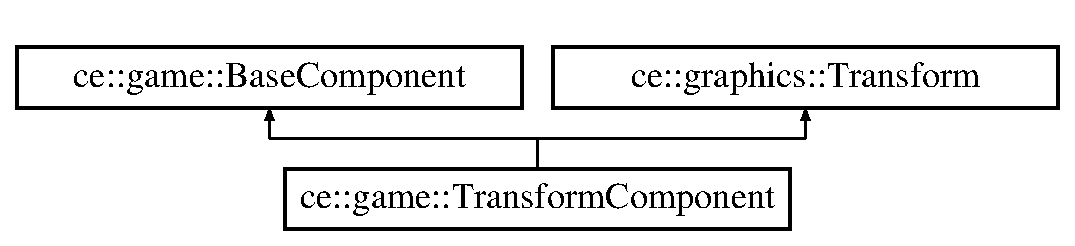
\includegraphics[height=2.000000cm]{classce_1_1game_1_1_transform_component}
\end{center}
\end{figure}
\subsection*{Public Member Functions}
\begin{DoxyCompactItemize}
\item 
\mbox{\Hypertarget{classce_1_1game_1_1_transform_component_a43c2bc090897e4581ebf0edf463d7c09}\label{classce_1_1game_1_1_transform_component_a43c2bc090897e4581ebf0edf463d7c09}} 
virtual void {\bfseries init} () override
\item 
\mbox{\Hypertarget{classce_1_1game_1_1_transform_component_afb2efbc69b503a59ebe4e0e6c8fc1b62}\label{classce_1_1game_1_1_transform_component_afb2efbc69b503a59ebe4e0e6c8fc1b62}} 
virtual void {\bfseries tick} (float dt) override
\item 
\mbox{\Hypertarget{classce_1_1game_1_1_transform_component_ad73ce4088d1771b2e28b8ce4f0ed9214}\label{classce_1_1game_1_1_transform_component_ad73ce4088d1771b2e28b8ce4f0ed9214}} 
virtual void {\bfseries draw} (\hyperlink{classce_1_1graphics_1_1_renderer3_d}{ce\+::graphics\+::\+Renderer3D} $\ast$renderer) override
\item 
virtual std\+::string \hyperlink{classce_1_1game_1_1_transform_component_ae4a2729b3f88a77b8405de317ab03510}{get\+Type} () override
\begin{DoxyCompactList}\small\item\em Returns the type of Component in a string value. \end{DoxyCompactList}\item 
\mbox{\Hypertarget{classce_1_1game_1_1_transform_component_aa5460c96774e9b00ec4bfadadb1ec1ce}\label{classce_1_1game_1_1_transform_component_aa5460c96774e9b00ec4bfadadb1ec1ce}} 
glm\+::mat4 \hyperlink{classce_1_1game_1_1_transform_component_aa5460c96774e9b00ec4bfadadb1ec1ce}{get\+As\+Model\+Matrix} ()
\begin{DoxyCompactList}\small\item\em Get the position, rotation and scale as a matrix for drawing etc. \end{DoxyCompactList}\item 
\mbox{\Hypertarget{classce_1_1game_1_1_transform_component_ad7b1abf547a1b3a592814c70d2b60523}\label{classce_1_1game_1_1_transform_component_ad7b1abf547a1b3a592814c70d2b60523}} 
void {\bfseries pitch} (float degrees)
\item 
\mbox{\Hypertarget{classce_1_1game_1_1_transform_component_afac531098bba8a0a4ea0130b7285dcdc}\label{classce_1_1game_1_1_transform_component_afac531098bba8a0a4ea0130b7285dcdc}} 
void {\bfseries yaw} (float degrees)
\item 
\mbox{\Hypertarget{classce_1_1game_1_1_transform_component_a82f0c177d9a1e80aba887b425176e5eb}\label{classce_1_1game_1_1_transform_component_a82f0c177d9a1e80aba887b425176e5eb}} 
void {\bfseries roll} (float degrees)
\item 
\mbox{\Hypertarget{classce_1_1game_1_1_transform_component_abedd2e90c27e8ef29cd95a60a22b1e14}\label{classce_1_1game_1_1_transform_component_abedd2e90c27e8ef29cd95a60a22b1e14}} 
void {\bfseries rotate} (float degX, float degY, float degZ)
\item 
\mbox{\Hypertarget{classce_1_1game_1_1_transform_component_a9384679e28827f0f9a52e6be3a8bc317}\label{classce_1_1game_1_1_transform_component_a9384679e28827f0f9a52e6be3a8bc317}} 
void {\bfseries rotate} (glm\+::vec3 degrees)
\item 
\mbox{\Hypertarget{classce_1_1game_1_1_transform_component_a5e352aa67cc23129e22971ef977c6c44}\label{classce_1_1game_1_1_transform_component_a5e352aa67cc23129e22971ef977c6c44}} 
void {\bfseries set\+Rotation} (float degX, float degY, float degZ)
\item 
\mbox{\Hypertarget{classce_1_1game_1_1_transform_component_a4f064913de8e60bd903bb7b22f1c31f0}\label{classce_1_1game_1_1_transform_component_a4f064913de8e60bd903bb7b22f1c31f0}} 
void {\bfseries set\+Rotation} (glm\+::vec3 degrees)
\item 
\mbox{\Hypertarget{classce_1_1game_1_1_transform_component_a50763a58cbd41a1425f3cde07439198d}\label{classce_1_1game_1_1_transform_component_a50763a58cbd41a1425f3cde07439198d}} 
glm\+::vec3 {\bfseries get\+Rotation} ()
\item 
\mbox{\Hypertarget{classce_1_1game_1_1_transform_component_a20d58c0dec20520fa1c9d7ee86942c31}\label{classce_1_1game_1_1_transform_component_a20d58c0dec20520fa1c9d7ee86942c31}} 
void {\bfseries move} (float x, float y, float z)
\item 
\mbox{\Hypertarget{classce_1_1game_1_1_transform_component_a7a2fec624b054f16e9d2077c8d5ff97c}\label{classce_1_1game_1_1_transform_component_a7a2fec624b054f16e9d2077c8d5ff97c}} 
void {\bfseries move} (glm\+::vec3 xyz)
\item 
\mbox{\Hypertarget{classce_1_1game_1_1_transform_component_aabc98984d7d7bf3b8b9d8cb39b9c6f40}\label{classce_1_1game_1_1_transform_component_aabc98984d7d7bf3b8b9d8cb39b9c6f40}} 
void {\bfseries set\+Position} (float x, float y, float z)
\item 
\mbox{\Hypertarget{classce_1_1game_1_1_transform_component_ac004e2eada2a498100407894de052f9d}\label{classce_1_1game_1_1_transform_component_ac004e2eada2a498100407894de052f9d}} 
void {\bfseries set\+Position} (glm\+::vec3 xyz)
\item 
\mbox{\Hypertarget{classce_1_1game_1_1_transform_component_ae61537497dc93afed6a0d24d106bd77a}\label{classce_1_1game_1_1_transform_component_ae61537497dc93afed6a0d24d106bd77a}} 
glm\+::vec3 {\bfseries get\+Position} ()
\item 
\mbox{\Hypertarget{classce_1_1game_1_1_transform_component_aa14fa9beaf944e5ca50bc171395ff4b1}\label{classce_1_1game_1_1_transform_component_aa14fa9beaf944e5ca50bc171395ff4b1}} 
void {\bfseries scale} (float x, float y, float z)
\item 
\mbox{\Hypertarget{classce_1_1game_1_1_transform_component_ad242b736f29e8998f4c629849b6167b0}\label{classce_1_1game_1_1_transform_component_ad242b736f29e8998f4c629849b6167b0}} 
void {\bfseries scale} (glm\+::vec3 xyz)
\item 
\mbox{\Hypertarget{classce_1_1game_1_1_transform_component_a86b2727e507a7888fb8c6a26123a7d8b}\label{classce_1_1game_1_1_transform_component_a86b2727e507a7888fb8c6a26123a7d8b}} 
void {\bfseries set\+Scale} (float x, float y, float z)
\item 
\mbox{\Hypertarget{classce_1_1game_1_1_transform_component_af5840084e9c65ac550c1b563a301c5ca}\label{classce_1_1game_1_1_transform_component_af5840084e9c65ac550c1b563a301c5ca}} 
void {\bfseries set\+Scale} (glm\+::vec3 xyz)
\item 
\mbox{\Hypertarget{classce_1_1game_1_1_transform_component_a0ddf26fc356dc2646575d65f3f628250}\label{classce_1_1game_1_1_transform_component_a0ddf26fc356dc2646575d65f3f628250}} 
glm\+::vec3 {\bfseries get\+Scale} ()
\end{DoxyCompactItemize}
\subsection*{Protected Attributes}
\begin{DoxyCompactItemize}
\item 
glm\+::vec3 \hyperlink{classce_1_1game_1_1_transform_component_a72b0b9f989fd7ddcecf0ebec18bd2076}{m\+\_\+position} = glm\+::vec3(0.\+0f, 0.\+0f, 0.\+0f)
\begin{DoxyCompactList}\small\item\em Our position vector. \end{DoxyCompactList}\item 
glm\+::vec3 \hyperlink{classce_1_1game_1_1_transform_component_af120345110ceff7bcf3b40d2ac1b0575}{m\+\_\+scale} = glm\+::vec3(1.\+0f, 1.\+0f, 1.\+0f)
\begin{DoxyCompactList}\small\item\em Our scale vector. \end{DoxyCompactList}\item 
glm\+::vec3 \hyperlink{classce_1_1game_1_1_transform_component_aacf1e75e976c54bb503448b6da534f63}{m\+\_\+rotation} = glm\+::vec3(0.\+0f, 0.\+0f, 0.\+0f)
\end{DoxyCompactItemize}
\subsection*{Additional Inherited Members}


\subsection{Member Function Documentation}
\mbox{\Hypertarget{classce_1_1game_1_1_transform_component_ae4a2729b3f88a77b8405de317ab03510}\label{classce_1_1game_1_1_transform_component_ae4a2729b3f88a77b8405de317ab03510}} 
\index{ce\+::game\+::\+Transform\+Component@{ce\+::game\+::\+Transform\+Component}!get\+Type@{get\+Type}}
\index{get\+Type@{get\+Type}!ce\+::game\+::\+Transform\+Component@{ce\+::game\+::\+Transform\+Component}}
\subsubsection{\texorpdfstring{get\+Type()}{getType()}}
{\footnotesize\ttfamily std\+::string ce\+::game\+::\+Transform\+Component\+::get\+Type (\begin{DoxyParamCaption}{ }\end{DoxyParamCaption})\hspace{0.3cm}{\ttfamily [override]}, {\ttfamily [virtual]}}



Returns the type of Component in a string value. 

Example\+: Model, Transform etc 

Implements \hyperlink{classce_1_1game_1_1_base_component_a1022b55c1926a019a2b3a71fb6b9150e}{ce\+::game\+::\+Base\+Component}.



\subsection{Member Data Documentation}
\mbox{\Hypertarget{classce_1_1game_1_1_transform_component_a72b0b9f989fd7ddcecf0ebec18bd2076}\label{classce_1_1game_1_1_transform_component_a72b0b9f989fd7ddcecf0ebec18bd2076}} 
\index{ce\+::game\+::\+Transform\+Component@{ce\+::game\+::\+Transform\+Component}!m\+\_\+position@{m\+\_\+position}}
\index{m\+\_\+position@{m\+\_\+position}!ce\+::game\+::\+Transform\+Component@{ce\+::game\+::\+Transform\+Component}}
\subsubsection{\texorpdfstring{m\+\_\+position}{m\_position}}
{\footnotesize\ttfamily glm\+::vec3 ce\+::game\+::\+Transform\+Component\+::m\+\_\+position = glm\+::vec3(0.\+0f, 0.\+0f, 0.\+0f)\hspace{0.3cm}{\ttfamily [protected]}}



Our position vector. 

Each axis represents the position on said axis \mbox{\Hypertarget{classce_1_1game_1_1_transform_component_aacf1e75e976c54bb503448b6da534f63}\label{classce_1_1game_1_1_transform_component_aacf1e75e976c54bb503448b6da534f63}} 
\index{ce\+::game\+::\+Transform\+Component@{ce\+::game\+::\+Transform\+Component}!m\+\_\+rotation@{m\+\_\+rotation}}
\index{m\+\_\+rotation@{m\+\_\+rotation}!ce\+::game\+::\+Transform\+Component@{ce\+::game\+::\+Transform\+Component}}
\subsubsection{\texorpdfstring{m\+\_\+rotation}{m\_rotation}}
{\footnotesize\ttfamily glm\+::vec3 ce\+::game\+::\+Transform\+Component\+::m\+\_\+rotation = glm\+::vec3(0.\+0f, 0.\+0f, 0.\+0f)\hspace{0.3cm}{\ttfamily [protected]}}

Our rotation vector in eular angles

Each axis represents the degrees of rotation on said axis \mbox{\Hypertarget{classce_1_1game_1_1_transform_component_af120345110ceff7bcf3b40d2ac1b0575}\label{classce_1_1game_1_1_transform_component_af120345110ceff7bcf3b40d2ac1b0575}} 
\index{ce\+::game\+::\+Transform\+Component@{ce\+::game\+::\+Transform\+Component}!m\+\_\+scale@{m\+\_\+scale}}
\index{m\+\_\+scale@{m\+\_\+scale}!ce\+::game\+::\+Transform\+Component@{ce\+::game\+::\+Transform\+Component}}
\subsubsection{\texorpdfstring{m\+\_\+scale}{m\_scale}}
{\footnotesize\ttfamily glm\+::vec3 ce\+::game\+::\+Transform\+Component\+::m\+\_\+scale = glm\+::vec3(1.\+0f, 1.\+0f, 1.\+0f)\hspace{0.3cm}{\ttfamily [protected]}}



Our scale vector. 

Each axis represents the scale on said axis 

The documentation for this class was generated from the following files\+:\begin{DoxyCompactItemize}
\item 
E\+:/\+Development/\+Game\+Engine/\+C\+Engine/src/\+Game/\+Components/Transform\+Component.\+h\item 
E\+:/\+Development/\+Game\+Engine/\+C\+Engine/src/\+Game/\+Components/Transform\+Component.\+cpp\end{DoxyCompactItemize}

\hypertarget{structce_1_1graphics_1_1_vertex}{}\section{ce\+:\+:graphics\+:\+:Vertex Struct Reference}
\label{structce_1_1graphics_1_1_vertex}\index{ce\+::graphics\+::\+Vertex@{ce\+::graphics\+::\+Vertex}}


A vertex structure.  




{\ttfamily \#include $<$Vertex.\+h$>$}

\subsection*{Public Attributes}
\begin{DoxyCompactItemize}
\item 
glm\+::vec3 \hyperlink{structce_1_1graphics_1_1_vertex_aa38ddb0b29a672e67e790869f38282ff}{position}
\item 
glm\+::vec3 \hyperlink{structce_1_1graphics_1_1_vertex_ac91e1a269df3e9a9a3a69543f1f68f4b}{normal}
\item 
glm\+::vec2 \hyperlink{structce_1_1graphics_1_1_vertex_a1dd8f6082878c241afc66226b3c45ea0}{texture\+Coord}
\end{DoxyCompactItemize}


\subsection{Detailed Description}
A vertex structure. 

Contains\+:
\begin{DoxyItemize}
\item position
\item normal vector
\item texture coordinate 
\end{DoxyItemize}

\subsection{Member Data Documentation}
\mbox{\Hypertarget{structce_1_1graphics_1_1_vertex_ac91e1a269df3e9a9a3a69543f1f68f4b}\label{structce_1_1graphics_1_1_vertex_ac91e1a269df3e9a9a3a69543f1f68f4b}} 
\index{ce\+::graphics\+::\+Vertex@{ce\+::graphics\+::\+Vertex}!normal@{normal}}
\index{normal@{normal}!ce\+::graphics\+::\+Vertex@{ce\+::graphics\+::\+Vertex}}
\subsubsection{\texorpdfstring{normal}{normal}}
{\footnotesize\ttfamily glm\+::vec3 ce\+::graphics\+::\+Vertex\+::normal}

A 3D vector describing this \hyperlink{structce_1_1graphics_1_1_vertex}{Vertex} normal \mbox{\Hypertarget{structce_1_1graphics_1_1_vertex_aa38ddb0b29a672e67e790869f38282ff}\label{structce_1_1graphics_1_1_vertex_aa38ddb0b29a672e67e790869f38282ff}} 
\index{ce\+::graphics\+::\+Vertex@{ce\+::graphics\+::\+Vertex}!position@{position}}
\index{position@{position}!ce\+::graphics\+::\+Vertex@{ce\+::graphics\+::\+Vertex}}
\subsubsection{\texorpdfstring{position}{position}}
{\footnotesize\ttfamily glm\+::vec3 ce\+::graphics\+::\+Vertex\+::position}

A 3D position, x, y, z \mbox{\Hypertarget{structce_1_1graphics_1_1_vertex_a1dd8f6082878c241afc66226b3c45ea0}\label{structce_1_1graphics_1_1_vertex_a1dd8f6082878c241afc66226b3c45ea0}} 
\index{ce\+::graphics\+::\+Vertex@{ce\+::graphics\+::\+Vertex}!texture\+Coord@{texture\+Coord}}
\index{texture\+Coord@{texture\+Coord}!ce\+::graphics\+::\+Vertex@{ce\+::graphics\+::\+Vertex}}
\subsubsection{\texorpdfstring{texture\+Coord}{textureCoord}}
{\footnotesize\ttfamily glm\+::vec2 ce\+::graphics\+::\+Vertex\+::texture\+Coord}

A 2D vector for texture coordinates 

The documentation for this struct was generated from the following file\+:\begin{DoxyCompactItemize}
\item 
E\+:/\+Development/\+Game\+Engine/\+C\+Engine/src/\+Graphics/\hyperlink{_vertex_8h}{Vertex.\+h}\end{DoxyCompactItemize}

\hypertarget{classce_1_1core_1_1_window}{}\section{ce\+:\+:core\+:\+:Window Class Reference}
\label{classce_1_1core_1_1_window}\index{ce\+::core\+::\+Window@{ce\+::core\+::\+Window}}


A window class that can be drawn to.  




{\ttfamily \#include $<$Window.\+h$>$}

\subsection*{Public Member Functions}
\begin{DoxyCompactItemize}
\item 
\hyperlink{classce_1_1core_1_1_window_a01f1749caa5bb182410a5abcd65e9528}{Window} (std\+::string title, int posx, int posy, int width, int height, unsigned int flags=W\+I\+N\+D\+O\+W\+\_\+\+S\+H\+O\+WN)
\begin{DoxyCompactList}\small\item\em Constructor for creating the window. \end{DoxyCompactList}\item 
void \hyperlink{classce_1_1core_1_1_window_a4bdfb3cf6986e6144546cdfeb4c19e6e}{create} (std\+::string title, int posx, int posy, int width, int height, unsigned int flags=W\+I\+N\+D\+O\+W\+\_\+\+S\+H\+O\+WN)
\begin{DoxyCompactList}\small\item\em Function for creating the window. \end{DoxyCompactList}\item 
void \hyperlink{classce_1_1core_1_1_window_a48c120ae2d7e03c6839747065eeeb7be}{set\+Clear\+Color} (float r, float g, float b, float a=0.\+0f)
\item 
void \hyperlink{classce_1_1core_1_1_window_ab47b3b317acbf0ba71f4e56bd2313f0d}{clear} ()
\item 
void \hyperlink{classce_1_1core_1_1_window_a9ec120e3e9031f86acaf5ac350a8b5e4}{display} ()
\item 
void \hyperlink{classce_1_1core_1_1_window_a105a93cc62e222c99411b3184b70d84a}{set\+Size} (int width, int height)
\begin{DoxyCompactList}\small\item\em Sets the window size. \end{DoxyCompactList}\item 
void \hyperlink{classce_1_1core_1_1_window_ac182b4657e4240663b49923e6349e48c}{set\+Title} (std\+::string title)
\begin{DoxyCompactList}\small\item\em Sets the window title. \end{DoxyCompactList}\item 
void \hyperlink{classce_1_1core_1_1_window_a40a91b63d87c6942dea3186fb4b05085}{set\+Window\+Grab} (bool grab)
\begin{DoxyCompactList}\small\item\em Sets the window grab. \end{DoxyCompactList}\item 
void \hyperlink{classce_1_1core_1_1_window_a9fafce9f3898b399c149a561d9ceac12}{set\+Window\+Fullscreen} (unsigned int type)
\begin{DoxyCompactList}\small\item\em Set fullscreen mode. \end{DoxyCompactList}\item 
glm\+::vec2 \hyperlink{classce_1_1core_1_1_window_abba818ed742e942c7d009c1c1fd7ecca}{get\+Size} ()
\end{DoxyCompactItemize}
\subsection*{Protected Member Functions}
\begin{DoxyCompactItemize}
\item 
\mbox{\Hypertarget{classce_1_1core_1_1_window_a03535243d5663e6f7432f2cba0888642}\label{classce_1_1core_1_1_window_a03535243d5663e6f7432f2cba0888642}} 
void {\bfseries init\+Video\+Components} ()
\item 
\mbox{\Hypertarget{classce_1_1core_1_1_window_aa29eebc80fdc4556365bc4c42e953a12}\label{classce_1_1core_1_1_window_aa29eebc80fdc4556365bc4c42e953a12}} 
void {\bfseries destroy\+Window} ()
\end{DoxyCompactItemize}
\subsection*{Protected Attributes}
\begin{DoxyCompactItemize}
\item 
\mbox{\Hypertarget{classce_1_1core_1_1_window_a84ff05cd18af48c99b59f661544f0a5c}\label{classce_1_1core_1_1_window_a84ff05cd18af48c99b59f661544f0a5c}} 
S\+D\+L\+\_\+\+Window $\ast$ {\bfseries m\+\_\+window} = nullptr
\item 
\mbox{\Hypertarget{classce_1_1core_1_1_window_ac218ede314fa261711eba26dbaabd4a7}\label{classce_1_1core_1_1_window_ac218ede314fa261711eba26dbaabd4a7}} 
S\+D\+L\+\_\+\+G\+L\+Context {\bfseries m\+\_\+gl\+Context} = N\+U\+LL
\end{DoxyCompactItemize}


\subsection{Detailed Description}
A window class that can be drawn to. 

\subsection{Constructor \& Destructor Documentation}
\mbox{\Hypertarget{classce_1_1core_1_1_window_a01f1749caa5bb182410a5abcd65e9528}\label{classce_1_1core_1_1_window_a01f1749caa5bb182410a5abcd65e9528}} 
\index{ce\+::core\+::\+Window@{ce\+::core\+::\+Window}!Window@{Window}}
\index{Window@{Window}!ce\+::core\+::\+Window@{ce\+::core\+::\+Window}}
\subsubsection{\texorpdfstring{Window()}{Window()}}
{\footnotesize\ttfamily ce\+::core\+::\+Window\+::\+Window (\begin{DoxyParamCaption}\item[{std\+::string}]{title,  }\item[{int}]{posx,  }\item[{int}]{posy,  }\item[{int}]{width,  }\item[{int}]{height,  }\item[{unsigned int}]{flags = {\ttfamily WINDOW\+\_\+SHOWN} }\end{DoxyParamCaption})}



Constructor for creating the window. 


\begin{DoxyParams}{Parameters}
{\em title} & \hyperlink{classce_1_1core_1_1_window}{Window} title \\
\hline
{\em posx} & \hyperlink{classce_1_1core_1_1_window}{Window} position x on screen (W\+I\+N\+D\+O\+W\+P\+O\+S\+\_\+\+C\+E\+N\+T\+E\+R\+ED for centered) \\
\hline
{\em posy} & \hyperlink{classce_1_1core_1_1_window}{Window} position y on screen (W\+I\+N\+D\+O\+W\+P\+O\+S\+\_\+\+C\+E\+N\+T\+E\+R\+ED for centered) \\
\hline
{\em width} & \hyperlink{classce_1_1core_1_1_window}{Window} width \\
\hline
{\em height} & \hyperlink{classce_1_1core_1_1_window}{Window} height \\
\hline
{\em flags} & Window\+Flags describing how the window should be created \\
\hline
\end{DoxyParams}


\subsection{Member Function Documentation}
\mbox{\Hypertarget{classce_1_1core_1_1_window_ab47b3b317acbf0ba71f4e56bd2313f0d}\label{classce_1_1core_1_1_window_ab47b3b317acbf0ba71f4e56bd2313f0d}} 
\index{ce\+::core\+::\+Window@{ce\+::core\+::\+Window}!clear@{clear}}
\index{clear@{clear}!ce\+::core\+::\+Window@{ce\+::core\+::\+Window}}
\subsubsection{\texorpdfstring{clear()}{clear()}}
{\footnotesize\ttfamily void ce\+::core\+::\+Window\+::clear (\begin{DoxyParamCaption}{ }\end{DoxyParamCaption})}

Clears window buffer with the set clear color \mbox{\Hypertarget{classce_1_1core_1_1_window_a4bdfb3cf6986e6144546cdfeb4c19e6e}\label{classce_1_1core_1_1_window_a4bdfb3cf6986e6144546cdfeb4c19e6e}} 
\index{ce\+::core\+::\+Window@{ce\+::core\+::\+Window}!create@{create}}
\index{create@{create}!ce\+::core\+::\+Window@{ce\+::core\+::\+Window}}
\subsubsection{\texorpdfstring{create()}{create()}}
{\footnotesize\ttfamily void ce\+::core\+::\+Window\+::create (\begin{DoxyParamCaption}\item[{std\+::string}]{title,  }\item[{int}]{posx,  }\item[{int}]{posy,  }\item[{int}]{width,  }\item[{int}]{height,  }\item[{unsigned int}]{flags = {\ttfamily WINDOW\+\_\+SHOWN} }\end{DoxyParamCaption})}



Function for creating the window. 


\begin{DoxyParams}{Parameters}
{\em title} & \hyperlink{classce_1_1core_1_1_window}{Window} title \\
\hline
{\em posx} & \hyperlink{classce_1_1core_1_1_window}{Window} position x on screen (W\+I\+N\+D\+O\+W\+P\+O\+S\+\_\+\+C\+E\+N\+T\+E\+R\+ED for centered) \\
\hline
{\em posy} & \hyperlink{classce_1_1core_1_1_window}{Window} position y on screen (W\+I\+N\+D\+O\+W\+P\+O\+S\+\_\+\+C\+E\+N\+T\+E\+R\+ED for centered) \\
\hline
{\em width} & \hyperlink{classce_1_1core_1_1_window}{Window} width \\
\hline
{\em height} & \hyperlink{classce_1_1core_1_1_window}{Window} height \\
\hline
{\em flags} & Window\+Flags describing how the window should be created \\
\hline
\end{DoxyParams}
\mbox{\Hypertarget{classce_1_1core_1_1_window_a9ec120e3e9031f86acaf5ac350a8b5e4}\label{classce_1_1core_1_1_window_a9ec120e3e9031f86acaf5ac350a8b5e4}} 
\index{ce\+::core\+::\+Window@{ce\+::core\+::\+Window}!display@{display}}
\index{display@{display}!ce\+::core\+::\+Window@{ce\+::core\+::\+Window}}
\subsubsection{\texorpdfstring{display()}{display()}}
{\footnotesize\ttfamily void ce\+::core\+::\+Window\+::display (\begin{DoxyParamCaption}{ }\end{DoxyParamCaption})}

Changes buffer behind the scene essentially displaying all that has been rendered \mbox{\Hypertarget{classce_1_1core_1_1_window_abba818ed742e942c7d009c1c1fd7ecca}\label{classce_1_1core_1_1_window_abba818ed742e942c7d009c1c1fd7ecca}} 
\index{ce\+::core\+::\+Window@{ce\+::core\+::\+Window}!get\+Size@{get\+Size}}
\index{get\+Size@{get\+Size}!ce\+::core\+::\+Window@{ce\+::core\+::\+Window}}
\subsubsection{\texorpdfstring{get\+Size()}{getSize()}}
{\footnotesize\ttfamily glm\+::vec2 ce\+::core\+::\+Window\+::get\+Size (\begin{DoxyParamCaption}{ }\end{DoxyParamCaption})}

Returns a vector with the width and height of the window \mbox{\Hypertarget{classce_1_1core_1_1_window_a48c120ae2d7e03c6839747065eeeb7be}\label{classce_1_1core_1_1_window_a48c120ae2d7e03c6839747065eeeb7be}} 
\index{ce\+::core\+::\+Window@{ce\+::core\+::\+Window}!set\+Clear\+Color@{set\+Clear\+Color}}
\index{set\+Clear\+Color@{set\+Clear\+Color}!ce\+::core\+::\+Window@{ce\+::core\+::\+Window}}
\subsubsection{\texorpdfstring{set\+Clear\+Color()}{setClearColor()}}
{\footnotesize\ttfamily void ce\+::core\+::\+Window\+::set\+Clear\+Color (\begin{DoxyParamCaption}\item[{float}]{r,  }\item[{float}]{g,  }\item[{float}]{b,  }\item[{float}]{a = {\ttfamily 0.0f} }\end{DoxyParamCaption})}

Sets the clearcolor for this window and its context


\begin{DoxyParams}{Parameters}
{\em r} & Red component (0.\+0f -\/ 1.\+0f) \\
\hline
{\em g} & Green component (0.\+0f -\/ 1.\+0f) \\
\hline
{\em b} & Blue component (0.\+0f -\/ 1.\+0f) \\
\hline
{\em a} & Alpha component (0.\+0f -\/ 1.\+0f) \\
\hline
\end{DoxyParams}
\mbox{\Hypertarget{classce_1_1core_1_1_window_a105a93cc62e222c99411b3184b70d84a}\label{classce_1_1core_1_1_window_a105a93cc62e222c99411b3184b70d84a}} 
\index{ce\+::core\+::\+Window@{ce\+::core\+::\+Window}!set\+Size@{set\+Size}}
\index{set\+Size@{set\+Size}!ce\+::core\+::\+Window@{ce\+::core\+::\+Window}}
\subsubsection{\texorpdfstring{set\+Size()}{setSize()}}
{\footnotesize\ttfamily void ce\+::core\+::\+Window\+::set\+Size (\begin{DoxyParamCaption}\item[{int}]{width,  }\item[{int}]{height }\end{DoxyParamCaption})}



Sets the window size. 


\begin{DoxyParams}{Parameters}
{\em width} & Width \\
\hline
{\em height} & Height \\
\hline
\end{DoxyParams}
\mbox{\Hypertarget{classce_1_1core_1_1_window_ac182b4657e4240663b49923e6349e48c}\label{classce_1_1core_1_1_window_ac182b4657e4240663b49923e6349e48c}} 
\index{ce\+::core\+::\+Window@{ce\+::core\+::\+Window}!set\+Title@{set\+Title}}
\index{set\+Title@{set\+Title}!ce\+::core\+::\+Window@{ce\+::core\+::\+Window}}
\subsubsection{\texorpdfstring{set\+Title()}{setTitle()}}
{\footnotesize\ttfamily void ce\+::core\+::\+Window\+::set\+Title (\begin{DoxyParamCaption}\item[{std\+::string}]{title }\end{DoxyParamCaption})}



Sets the window title. 


\begin{DoxyParams}{Parameters}
{\em title} & Title \\
\hline
\end{DoxyParams}
\mbox{\Hypertarget{classce_1_1core_1_1_window_a9fafce9f3898b399c149a561d9ceac12}\label{classce_1_1core_1_1_window_a9fafce9f3898b399c149a561d9ceac12}} 
\index{ce\+::core\+::\+Window@{ce\+::core\+::\+Window}!set\+Window\+Fullscreen@{set\+Window\+Fullscreen}}
\index{set\+Window\+Fullscreen@{set\+Window\+Fullscreen}!ce\+::core\+::\+Window@{ce\+::core\+::\+Window}}
\subsubsection{\texorpdfstring{set\+Window\+Fullscreen()}{setWindowFullscreen()}}
{\footnotesize\ttfamily void ce\+::core\+::\+Window\+::set\+Window\+Fullscreen (\begin{DoxyParamCaption}\item[{unsigned int}]{type }\end{DoxyParamCaption})}



Set fullscreen mode. 


\begin{DoxyParams}{Parameters}
{\em type} & Should be either W\+I\+N\+D\+O\+W\+\_\+\+F\+U\+L\+L\+S\+C\+R\+E\+EN, W\+I\+N\+D\+O\+W\+\_\+\+F\+U\+L\+L\+S\+C\+R\+E\+E\+N\+\_\+\+D\+E\+S\+K\+T\+OP or 0 to set back to windowed \\
\hline
\end{DoxyParams}
\mbox{\Hypertarget{classce_1_1core_1_1_window_a40a91b63d87c6942dea3186fb4b05085}\label{classce_1_1core_1_1_window_a40a91b63d87c6942dea3186fb4b05085}} 
\index{ce\+::core\+::\+Window@{ce\+::core\+::\+Window}!set\+Window\+Grab@{set\+Window\+Grab}}
\index{set\+Window\+Grab@{set\+Window\+Grab}!ce\+::core\+::\+Window@{ce\+::core\+::\+Window}}
\subsubsection{\texorpdfstring{set\+Window\+Grab()}{setWindowGrab()}}
{\footnotesize\ttfamily void ce\+::core\+::\+Window\+::set\+Window\+Grab (\begin{DoxyParamCaption}\item[{bool}]{grab }\end{DoxyParamCaption})}



Sets the window grab. 

Essentially tell the window to hide the cursor and keep it inside the bounds of the window.


\begin{DoxyParams}{Parameters}
{\em grab} & Decides if window should grab the cursor or not \\
\hline
\end{DoxyParams}


The documentation for this class was generated from the following files\+:\begin{DoxyCompactItemize}
\item 
Core/\hyperlink{_window_8h}{Window.\+h}\item 
Core/Window.\+cpp\end{DoxyCompactItemize}

\chapter{File Documentation}
\hypertarget{_application_8h}{}\section{E\+:/\+Development/\+Game\+Engine/\+C\+Engine/src/\+Core/\+Application.h File Reference}
\label{_application_8h}\index{E\+:/\+Development/\+Game\+Engine/\+C\+Engine/src/\+Core/\+Application.\+h@{E\+:/\+Development/\+Game\+Engine/\+C\+Engine/src/\+Core/\+Application.\+h}}
{\ttfamily \#include \char`\"{}S\+D\+L2/\+S\+D\+L.\+h\char`\"{}}\newline
{\ttfamily \#include \char`\"{}Core/\+Utility/log.\+h\char`\"{}}\newline
{\ttfamily \#include $<$iostream$>$}\newline
{\ttfamily \#include $<$string$>$}\newline
\subsection*{Classes}
\begin{DoxyCompactItemize}
\item 
class \hyperlink{classce_1_1core_1_1_application}{ce\+::core\+::\+Application}
\begin{DoxyCompactList}\small\item\em \hyperlink{classce_1_1core_1_1_application}{Application} singlton containing context info needed by some components. \end{DoxyCompactList}\end{DoxyCompactItemize}

\hypertarget{_input_8h}{}\section{E\+:/\+Development/\+Game\+Engine/\+C\+Engine/src/\+Core/\+Input.h File Reference}
\label{_input_8h}\index{E\+:/\+Development/\+Game\+Engine/\+C\+Engine/src/\+Core/\+Input.\+h@{E\+:/\+Development/\+Game\+Engine/\+C\+Engine/src/\+Core/\+Input.\+h}}
{\ttfamily \#include $<$functional$>$}\newline
{\ttfamily \#include $<$unordered\+\_\+map$>$}\newline
{\ttfamily \#include $<$vector$>$}\newline
{\ttfamily \#include $<$iostream$>$}\newline
{\ttfamily \#include \char`\"{}S\+D\+L2/\+S\+D\+L.\+h\char`\"{}}\newline
{\ttfamily \#include \char`\"{}Core/\+Utility/log.\+h\char`\"{}}\newline
{\ttfamily \#include \char`\"{}Input\+Codes.\+h\char`\"{}}\newline
\subsection*{Classes}
\begin{DoxyCompactItemize}
\item 
struct \hyperlink{structce_1_1core_1_1_joystick}{ce\+::core\+::\+Joystick}
\begin{DoxyCompactList}\small\item\em Structure containing information needed for Joysticks and Controllers. \end{DoxyCompactList}\item 
class \hyperlink{classce_1_1core_1_1_input}{ce\+::core\+::\+Input}
\begin{DoxyCompactList}\small\item\em Class for handling user input. \end{DoxyCompactList}\end{DoxyCompactItemize}

\hypertarget{_input_codes_8h}{}\section{Core/\+Input\+Codes.h File Reference}
\label{_input_codes_8h}\index{Core/\+Input\+Codes.\+h@{Core/\+Input\+Codes.\+h}}


Contains all the input codes for buttons and axis\textquotesingle{}s.  


{\ttfamily \#include \char`\"{}S\+D\+L2/\+S\+D\+L.\+h\char`\"{}}\newline
\subsection*{Enumerations}
\begin{DoxyCompactItemize}
\item 
enum \hyperlink{_input_codes_8h_a9044fffd6a7c3417b0a100f0a0427a90}{ce\+::core\+::\+Axis\+Event\+Codes} \{ \newline
\hyperlink{_input_codes_8h_a9044fffd6a7c3417b0a100f0a0427a90a8d73683d889e31faf0662fd201794c90}{ce\+::core\+::\+M\+\_\+\+M\+O\+T\+I\+O\+N\+\_\+X} = 0x01, 
\hyperlink{_input_codes_8h_a9044fffd6a7c3417b0a100f0a0427a90a48d1908e0caf112a71aeb5febefb14a5}{ce\+::core\+::\+M\+\_\+\+M\+O\+T\+I\+O\+N\+\_\+Y} = 0x02, 
\hyperlink{_input_codes_8h_a9044fffd6a7c3417b0a100f0a0427a90ab2795023ce2458199f937e927285cce9}{ce\+::core\+::\+M\+\_\+\+M\+O\+T\+I\+O\+N\+\_\+\+X\+R\+EL} = 0x03, 
\hyperlink{_input_codes_8h_a9044fffd6a7c3417b0a100f0a0427a90adae46ff6b1b43c48f30733c388ca16d6}{ce\+::core\+::\+M\+\_\+\+M\+O\+T\+I\+O\+N\+\_\+\+Y\+R\+EL} = 0x04, 
\newline
\hyperlink{_input_codes_8h_a9044fffd6a7c3417b0a100f0a0427a90a2a35fb3465f9999b04b6fc05d3387875}{ce\+::core\+::\+M\+\_\+\+W\+H\+E\+E\+L\+\_\+X} = 0x05, 
\hyperlink{_input_codes_8h_a9044fffd6a7c3417b0a100f0a0427a90ae35cd013aca44f2613cda6b51035ac2e}{ce\+::core\+::\+M\+\_\+\+W\+H\+E\+E\+L\+\_\+Y} = 0x06, 
\hyperlink{_input_codes_8h_a9044fffd6a7c3417b0a100f0a0427a90a94ac650a340e4ce244cadd4dc10da269}{ce\+::core\+::\+C\+\_\+\+A\+X\+I\+S\+\_\+\+L\+S\+T\+I\+C\+KX} = 0x07, 
\hyperlink{_input_codes_8h_a9044fffd6a7c3417b0a100f0a0427a90ab661f75e284d4046ef4fc557da826bdb}{ce\+::core\+::\+C\+\_\+\+A\+X\+I\+S\+\_\+\+L\+S\+T\+I\+C\+KY} = 0x08, 
\newline
\hyperlink{_input_codes_8h_a9044fffd6a7c3417b0a100f0a0427a90a7ba4849f64fa212cc2f23d329c2d7d18}{ce\+::core\+::\+C\+\_\+\+A\+X\+I\+S\+\_\+\+R\+S\+T\+I\+C\+KX} = 0x09, 
\hyperlink{_input_codes_8h_a9044fffd6a7c3417b0a100f0a0427a90ad38af62a307ddc10bab199d1bbbb81e8}{ce\+::core\+::\+C\+\_\+\+A\+X\+I\+S\+\_\+\+R\+S\+T\+I\+C\+KY} = 0x0A, 
\hyperlink{_input_codes_8h_a9044fffd6a7c3417b0a100f0a0427a90aa208cbe26c203351be9db721bd796c3a}{ce\+::core\+::\+C\+\_\+\+A\+X\+I\+S\+\_\+\+L\+T\+R\+I\+G\+G\+ER} = 0x0B, 
\hyperlink{_input_codes_8h_a9044fffd6a7c3417b0a100f0a0427a90a6004060112b6b9af602e67c3f1abaac5}{ce\+::core\+::\+C\+\_\+\+A\+X\+I\+S\+\_\+\+R\+T\+R\+I\+G\+G\+ER} = 0x0C
 \}\begin{DoxyCompactList}\small\item\em Enum containing all the codes for detecting Axis\+Events such as the mouse. \end{DoxyCompactList}
\item 
enum \hyperlink{_input_codes_8h_a0205e42a827583bec00e09861c1bd835}{ce\+::core\+::\+Key\+Codes} \{ \newline
\hyperlink{_input_codes_8h_a0205e42a827583bec00e09861c1bd835a541ae720b68e0b2a112777ef8c04664a}{ce\+::core\+::\+C\+\_\+\+B\+U\+T\+T\+O\+N\+\_\+\+F\+A\+C\+E1} = -\/100000, 
\hyperlink{_input_codes_8h_a0205e42a827583bec00e09861c1bd835a975abced915152d9c51ea78b7e90805b}{ce\+::core\+::\+C\+\_\+\+B\+U\+T\+T\+O\+N\+\_\+\+F\+A\+C\+E2} = -\/100001, 
\hyperlink{_input_codes_8h_a0205e42a827583bec00e09861c1bd835a7fcd7bda7929ea20b455a1913b192314}{ce\+::core\+::\+C\+\_\+\+B\+U\+T\+T\+O\+N\+\_\+\+F\+A\+C\+E3} = -\/100002, 
\hyperlink{_input_codes_8h_a0205e42a827583bec00e09861c1bd835a709c61fd5fc4b773111543e14310e473}{ce\+::core\+::\+C\+\_\+\+B\+U\+T\+T\+O\+N\+\_\+\+F\+A\+C\+E4} = -\/100003, 
\newline
\hyperlink{_input_codes_8h_a0205e42a827583bec00e09861c1bd835a6b019cd4311010cdc5f767d300aa3b9d}{ce\+::core\+::\+C\+\_\+\+B\+U\+T\+T\+O\+N\+\_\+\+D\+P\+A\+D\+\_\+\+D\+O\+WN} = -\/100004, 
\hyperlink{_input_codes_8h_a0205e42a827583bec00e09861c1bd835acdc9d81757be3eeb048a8410a4e394e4}{ce\+::core\+::\+C\+\_\+\+B\+U\+T\+T\+O\+N\+\_\+\+D\+P\+A\+D\+\_\+\+UP} = -\/100005, 
\hyperlink{_input_codes_8h_a0205e42a827583bec00e09861c1bd835a97852326dcfccd0c440d9966eea149c9}{ce\+::core\+::\+C\+\_\+\+B\+U\+T\+T\+O\+N\+\_\+\+D\+P\+A\+D\+\_\+\+L\+E\+FT} = -\/100006, 
\hyperlink{_input_codes_8h_a0205e42a827583bec00e09861c1bd835a10ac87964758ef67ea9c9f2535b3da34}{ce\+::core\+::\+C\+\_\+\+B\+U\+T\+T\+O\+N\+\_\+\+D\+P\+A\+D\+\_\+\+R\+I\+G\+HT} = -\/100007, 
\newline
\hyperlink{_input_codes_8h_a0205e42a827583bec00e09861c1bd835ad50144a13358e8f5114ff804a2e55423}{ce\+::core\+::\+C\+\_\+\+B\+U\+T\+T\+O\+N\+\_\+\+S\+T\+I\+C\+K1} = -\/100008, 
\hyperlink{_input_codes_8h_a0205e42a827583bec00e09861c1bd835a0f222616f48720f9bdf1e8aeddfd6392}{ce\+::core\+::\+C\+\_\+\+B\+U\+T\+T\+O\+N\+\_\+\+S\+T\+I\+C\+K2} = -\/100009, 
\hyperlink{_input_codes_8h_a0205e42a827583bec00e09861c1bd835aa6b81937de4493647ece034ec2d8fbdf}{ce\+::core\+::\+C\+\_\+\+B\+U\+T\+T\+O\+N\+\_\+\+L\+B\+U\+M\+P\+ER} = -\/100010, 
\hyperlink{_input_codes_8h_a0205e42a827583bec00e09861c1bd835a8b3608b5d5914bd84f52bfd55c1493e6}{ce\+::core\+::\+C\+\_\+\+B\+U\+T\+T\+O\+N\+\_\+\+R\+B\+U\+M\+P\+ER} = -\/100011, 
\newline
\hyperlink{_input_codes_8h_a0205e42a827583bec00e09861c1bd835ad91a31bc4c9a66c21e59381d7c0baa74}{ce\+::core\+::\+C\+\_\+\+B\+U\+T\+T\+O\+N\+\_\+\+S\+E\+L\+E\+CT} = -\/100012, 
\hyperlink{_input_codes_8h_a0205e42a827583bec00e09861c1bd835a59b6e2a3d84514da2c3b552c65057b78}{ce\+::core\+::\+C\+\_\+\+B\+U\+T\+T\+O\+N\+\_\+\+S\+T\+A\+RT} = -\/100013, 
\hyperlink{_input_codes_8h_a0205e42a827583bec00e09861c1bd835a9f07d6a4f9da6b0a35dec260e4f54a49}{ce\+::core\+::\+M\+\_\+\+B\+U\+T\+T\+O\+N\+\_\+\+L\+E\+FT} = -\/10000, 
\hyperlink{_input_codes_8h_a0205e42a827583bec00e09861c1bd835a8568da306dbe722b0aece6760be3d544}{ce\+::core\+::\+M\+\_\+\+B\+U\+T\+T\+O\+N\+\_\+\+R\+I\+G\+HT} = -\/10001, 
\newline
\hyperlink{_input_codes_8h_a0205e42a827583bec00e09861c1bd835a84fa491cc2a117c8eb03eb90b7a12d60}{ce\+::core\+::\+M\+\_\+\+B\+U\+T\+T\+O\+N\+\_\+\+M\+I\+D\+D\+LE} = -\/10002, 
\hyperlink{_input_codes_8h_a0205e42a827583bec00e09861c1bd835ac091a18aabe1eeaf5dc6f9b86cc3b5e8}{ce\+::core\+::\+M\+\_\+\+B\+U\+T\+T\+O\+N\+\_\+\+X1} = -\/10003, 
\hyperlink{_input_codes_8h_a0205e42a827583bec00e09861c1bd835aff901c73f428db5f1eb0ccda29275e5f}{ce\+::core\+::\+M\+\_\+\+B\+U\+T\+T\+O\+N\+\_\+\+X2} = -\/10004, 
{\bfseries K\+\_\+\+R\+E\+T\+U\+RN} = S\+D\+L\+K\+\_\+\+R\+E\+T\+U\+RN, 
\newline
{\bfseries K\+\_\+\+E\+S\+C\+A\+PE} = S\+D\+L\+K\+\_\+\+E\+S\+C\+A\+PE, 
{\bfseries K\+\_\+\+B\+A\+C\+K\+S\+P\+A\+CE} = S\+D\+L\+K\+\_\+\+B\+A\+C\+K\+S\+P\+A\+CE, 
{\bfseries K\+\_\+\+T\+AB} = S\+D\+L\+K\+\_\+\+T\+AB, 
{\bfseries K\+\_\+\+S\+P\+A\+CE} = S\+D\+L\+K\+\_\+\+S\+P\+A\+CE, 
\newline
{\bfseries K\+\_\+\+E\+X\+C\+L\+A\+IM} = S\+D\+L\+K\+\_\+\+E\+X\+C\+L\+A\+IM, 
{\bfseries K\+\_\+\+Q\+U\+O\+T\+E\+D\+BL} = S\+D\+L\+K\+\_\+\+Q\+U\+O\+T\+E\+D\+BL, 
{\bfseries K\+\_\+\+H\+A\+SH} = S\+D\+L\+K\+\_\+\+H\+A\+SH, 
{\bfseries K\+\_\+\+P\+E\+R\+C\+E\+NT} = S\+D\+L\+K\+\_\+\+P\+E\+R\+C\+E\+NT, 
\newline
{\bfseries K\+\_\+\+D\+O\+L\+L\+AR} = S\+D\+L\+K\+\_\+\+D\+O\+L\+L\+AR, 
{\bfseries K\+\_\+\+A\+M\+P\+E\+R\+S\+A\+ND} = S\+D\+L\+K\+\_\+\+A\+M\+P\+E\+R\+S\+A\+ND, 
{\bfseries K\+\_\+\+Q\+U\+O\+TE} = S\+D\+L\+K\+\_\+\+Q\+U\+O\+TE, 
{\bfseries K\+\_\+\+L\+E\+F\+T\+P\+A\+R\+EN} = S\+D\+L\+K\+\_\+\+L\+E\+F\+T\+P\+A\+R\+EN, 
\newline
{\bfseries K\+\_\+\+R\+I\+G\+H\+T\+P\+A\+R\+EN} = S\+D\+L\+K\+\_\+\+R\+I\+G\+H\+T\+P\+A\+R\+EN, 
{\bfseries K\+\_\+\+A\+S\+T\+E\+R\+I\+SK} = S\+D\+L\+K\+\_\+\+A\+S\+T\+E\+R\+I\+SK, 
{\bfseries K\+\_\+\+P\+L\+US} = S\+D\+L\+K\+\_\+\+P\+L\+US, 
{\bfseries K\+\_\+\+C\+O\+M\+MA} = S\+D\+L\+K\+\_\+\+C\+O\+M\+MA, 
\newline
{\bfseries K\+\_\+\+M\+I\+N\+US} = S\+D\+L\+K\+\_\+\+M\+I\+N\+US, 
{\bfseries K\+\_\+\+P\+E\+R\+I\+OD} = S\+D\+L\+K\+\_\+\+P\+E\+R\+I\+OD, 
{\bfseries K\+\_\+\+S\+L\+A\+SH} = S\+D\+L\+K\+\_\+\+S\+L\+A\+SH, 
{\bfseries K\+\_\+0} = S\+D\+L\+K\+\_\+0, 
\newline
{\bfseries K\+\_\+1} = S\+D\+L\+K\+\_\+1, 
{\bfseries K\+\_\+2} = S\+D\+L\+K\+\_\+2, 
{\bfseries K\+\_\+3} = S\+D\+L\+K\+\_\+3, 
{\bfseries K\+\_\+4} = S\+D\+L\+K\+\_\+4, 
\newline
{\bfseries K\+\_\+5} = S\+D\+L\+K\+\_\+5, 
{\bfseries K\+\_\+6} = S\+D\+L\+K\+\_\+6, 
{\bfseries K\+\_\+7} = S\+D\+L\+K\+\_\+7, 
{\bfseries K\+\_\+8} = S\+D\+L\+K\+\_\+8, 
\newline
{\bfseries K\+\_\+9} = S\+D\+L\+K\+\_\+9, 
{\bfseries K\+\_\+\+C\+O\+L\+ON} = S\+D\+L\+K\+\_\+\+C\+O\+L\+ON, 
{\bfseries K\+\_\+\+S\+E\+M\+I\+C\+O\+L\+ON} = S\+D\+L\+K\+\_\+\+S\+E\+M\+I\+C\+O\+L\+ON, 
{\bfseries K\+\_\+\+L\+E\+SS} = S\+D\+L\+K\+\_\+\+L\+E\+SS, 
\newline
{\bfseries K\+\_\+\+E\+Q\+U\+A\+LS} = S\+D\+L\+K\+\_\+\+E\+Q\+U\+A\+LS, 
{\bfseries K\+\_\+\+G\+R\+E\+A\+T\+ER} = S\+D\+L\+K\+\_\+\+G\+R\+E\+A\+T\+ER, 
{\bfseries K\+\_\+\+Q\+U\+E\+S\+T\+I\+ON} = S\+D\+L\+K\+\_\+\+Q\+U\+E\+S\+T\+I\+ON, 
{\bfseries K\+\_\+\+AT} = S\+D\+L\+K\+\_\+\+AT, 
\newline
{\bfseries K\+\_\+\+L\+E\+F\+T\+B\+R\+A\+C\+K\+ET} = S\+D\+L\+K\+\_\+\+L\+E\+F\+T\+B\+R\+A\+C\+K\+ET, 
{\bfseries K\+\_\+\+B\+A\+C\+K\+S\+L\+A\+SH} = S\+D\+L\+K\+\_\+\+B\+A\+C\+K\+S\+L\+A\+SH, 
{\bfseries K\+\_\+\+R\+I\+G\+H\+T\+B\+R\+A\+C\+K\+ET} = S\+D\+L\+K\+\_\+\+R\+I\+G\+H\+T\+B\+R\+A\+C\+K\+ET, 
{\bfseries K\+\_\+\+C\+A\+R\+ET} = S\+D\+L\+K\+\_\+\+C\+A\+R\+ET, 
\newline
{\bfseries K\+\_\+\+U\+N\+D\+E\+R\+S\+C\+O\+RE} = S\+D\+L\+K\+\_\+\+U\+N\+D\+E\+R\+S\+C\+O\+RE, 
{\bfseries K\+\_\+\+B\+A\+C\+K\+Q\+U\+O\+TE} = S\+D\+L\+K\+\_\+\+B\+A\+C\+K\+Q\+U\+O\+TE, 
{\bfseries K\+\_\+a} = S\+D\+L\+K\+\_\+a, 
{\bfseries K\+\_\+b} = S\+D\+L\+K\+\_\+b, 
\newline
{\bfseries K\+\_\+c} = S\+D\+L\+K\+\_\+c, 
{\bfseries K\+\_\+d} = S\+D\+L\+K\+\_\+d, 
{\bfseries K\+\_\+e} = S\+D\+L\+K\+\_\+e, 
{\bfseries K\+\_\+f} = S\+D\+L\+K\+\_\+f, 
\newline
{\bfseries K\+\_\+g} = S\+D\+L\+K\+\_\+g, 
{\bfseries K\+\_\+h} = S\+D\+L\+K\+\_\+h, 
{\bfseries K\+\_\+i} = S\+D\+L\+K\+\_\+i, 
{\bfseries K\+\_\+j} = S\+D\+L\+K\+\_\+j, 
\newline
{\bfseries K\+\_\+k} = S\+D\+L\+K\+\_\+k, 
{\bfseries K\+\_\+l} = S\+D\+L\+K\+\_\+l, 
{\bfseries K\+\_\+m} = S\+D\+L\+K\+\_\+m, 
{\bfseries K\+\_\+n} = S\+D\+L\+K\+\_\+n, 
\newline
{\bfseries K\+\_\+o} = S\+D\+L\+K\+\_\+o, 
{\bfseries K\+\_\+p} = S\+D\+L\+K\+\_\+p, 
{\bfseries K\+\_\+q} = S\+D\+L\+K\+\_\+q, 
{\bfseries K\+\_\+r} = S\+D\+L\+K\+\_\+r, 
\newline
{\bfseries K\+\_\+s} = S\+D\+L\+K\+\_\+s, 
{\bfseries K\+\_\+t} = S\+D\+L\+K\+\_\+t, 
{\bfseries K\+\_\+u} = S\+D\+L\+K\+\_\+u, 
{\bfseries K\+\_\+v} = S\+D\+L\+K\+\_\+v, 
\newline
{\bfseries K\+\_\+w} = S\+D\+L\+K\+\_\+w, 
{\bfseries K\+\_\+x} = S\+D\+L\+K\+\_\+x, 
{\bfseries K\+\_\+y} = S\+D\+L\+K\+\_\+y, 
{\bfseries K\+\_\+z} = S\+D\+L\+K\+\_\+z, 
\newline
{\bfseries K\+\_\+\+C\+A\+P\+S\+L\+O\+CK} = S\+D\+L\+K\+\_\+\+C\+A\+P\+S\+L\+O\+CK, 
{\bfseries K\+\_\+\+F1} = S\+D\+L\+K\+\_\+\+F1, 
{\bfseries K\+\_\+\+F2} = S\+D\+L\+K\+\_\+\+F2, 
{\bfseries K\+\_\+\+F3} = S\+D\+L\+K\+\_\+\+F3, 
\newline
{\bfseries K\+\_\+\+F4} = S\+D\+L\+K\+\_\+\+F4, 
{\bfseries K\+\_\+\+F5} = S\+D\+L\+K\+\_\+\+F5, 
{\bfseries K\+\_\+\+F6} = S\+D\+L\+K\+\_\+\+F6, 
{\bfseries K\+\_\+\+F7} = S\+D\+L\+K\+\_\+\+F7, 
\newline
{\bfseries K\+\_\+\+F8} = S\+D\+L\+K\+\_\+\+F8, 
{\bfseries K\+\_\+\+F9} = S\+D\+L\+K\+\_\+\+F9, 
{\bfseries K\+\_\+\+F10} = S\+D\+L\+K\+\_\+\+F10, 
{\bfseries K\+\_\+\+F11} = S\+D\+L\+K\+\_\+\+F11, 
\newline
{\bfseries K\+\_\+\+F12} = S\+D\+L\+K\+\_\+\+F12, 
{\bfseries K\+\_\+\+P\+R\+I\+N\+T\+S\+C\+R\+E\+EN} = S\+D\+L\+K\+\_\+\+P\+R\+I\+N\+T\+S\+C\+R\+E\+EN, 
{\bfseries K\+\_\+\+S\+C\+R\+O\+L\+L\+L\+O\+CK} = S\+D\+L\+K\+\_\+\+S\+C\+R\+O\+L\+L\+L\+O\+CK, 
{\bfseries K\+\_\+\+P\+A\+U\+SE} = S\+D\+L\+K\+\_\+\+P\+A\+U\+SE, 
\newline
{\bfseries K\+\_\+\+I\+N\+S\+E\+RT} = S\+D\+L\+K\+\_\+\+I\+N\+S\+E\+RT, 
{\bfseries K\+\_\+\+H\+O\+ME} = S\+D\+L\+K\+\_\+\+H\+O\+ME, 
{\bfseries K\+\_\+\+P\+A\+G\+E\+UP} = S\+D\+L\+K\+\_\+\+P\+A\+G\+E\+UP, 
{\bfseries K\+\_\+\+D\+E\+L\+E\+TE} = S\+D\+L\+K\+\_\+\+D\+E\+L\+E\+TE, 
\newline
{\bfseries K\+\_\+\+E\+ND} = S\+D\+L\+K\+\_\+\+E\+ND, 
{\bfseries K\+\_\+\+P\+A\+G\+E\+D\+O\+WN} = S\+D\+L\+K\+\_\+\+P\+A\+G\+E\+D\+O\+WN, 
{\bfseries K\+\_\+\+R\+I\+G\+HT} = S\+D\+L\+K\+\_\+\+R\+I\+G\+HT, 
{\bfseries K\+\_\+\+L\+E\+FT} = S\+D\+L\+K\+\_\+\+L\+E\+FT, 
\newline
{\bfseries K\+\_\+\+D\+O\+WN} = S\+D\+L\+K\+\_\+\+D\+O\+WN, 
{\bfseries K\+\_\+\+UP} = S\+D\+L\+K\+\_\+\+UP, 
{\bfseries K\+\_\+\+N\+U\+M\+L\+O\+C\+K\+C\+L\+E\+AR} = S\+D\+L\+K\+\_\+\+N\+U\+M\+L\+O\+C\+K\+C\+L\+E\+AR, 
{\bfseries K\+\_\+\+K\+P\+\_\+\+D\+I\+V\+I\+DE} = S\+D\+L\+K\+\_\+\+K\+P\+\_\+\+D\+I\+V\+I\+DE, 
\newline
{\bfseries K\+\_\+\+K\+P\+\_\+\+M\+U\+L\+T\+I\+P\+LY} = S\+D\+L\+K\+\_\+\+K\+P\+\_\+\+M\+U\+L\+T\+I\+P\+LY, 
{\bfseries K\+\_\+\+K\+P\+\_\+\+M\+I\+N\+US} = S\+D\+L\+K\+\_\+\+K\+P\+\_\+\+M\+I\+N\+US, 
{\bfseries K\+\_\+\+K\+P\+\_\+\+P\+L\+US} = S\+D\+L\+K\+\_\+\+K\+P\+\_\+\+P\+L\+US, 
{\bfseries K\+\_\+\+K\+P\+\_\+\+E\+N\+T\+ER} = S\+D\+L\+K\+\_\+\+K\+P\+\_\+\+E\+N\+T\+ER, 
\newline
{\bfseries K\+\_\+\+K\+P\+\_\+1} = S\+D\+L\+K\+\_\+\+K\+P\+\_\+1, 
{\bfseries K\+\_\+\+K\+P\+\_\+2} = S\+D\+L\+K\+\_\+\+K\+P\+\_\+2, 
{\bfseries K\+\_\+\+K\+P\+\_\+3} = S\+D\+L\+K\+\_\+\+K\+P\+\_\+3, 
{\bfseries K\+\_\+\+K\+P\+\_\+4} = S\+D\+L\+K\+\_\+\+K\+P\+\_\+4, 
\newline
{\bfseries K\+\_\+\+K\+P\+\_\+5} = S\+D\+L\+K\+\_\+\+K\+P\+\_\+5, 
{\bfseries K\+\_\+\+K\+P\+\_\+6} = S\+D\+L\+K\+\_\+\+K\+P\+\_\+6, 
{\bfseries K\+\_\+\+K\+P\+\_\+7} = S\+D\+L\+K\+\_\+\+K\+P\+\_\+7, 
{\bfseries K\+\_\+\+K\+P\+\_\+8} = S\+D\+L\+K\+\_\+\+K\+P\+\_\+8, 
\newline
{\bfseries K\+\_\+\+K\+P\+\_\+9} = S\+D\+L\+K\+\_\+\+K\+P\+\_\+9, 
{\bfseries K\+\_\+\+K\+P\+\_\+0} = S\+D\+L\+K\+\_\+\+K\+P\+\_\+0, 
{\bfseries K\+\_\+\+K\+P\+\_\+\+P\+E\+R\+I\+OD} = S\+D\+L\+K\+\_\+\+K\+P\+\_\+\+P\+E\+R\+I\+OD, 
{\bfseries K\+\_\+\+A\+P\+P\+L\+I\+C\+A\+T\+I\+ON} = S\+D\+L\+K\+\_\+\+A\+P\+P\+L\+I\+C\+A\+T\+I\+ON, 
\newline
{\bfseries K\+\_\+\+P\+O\+W\+ER} = S\+D\+L\+K\+\_\+\+P\+O\+W\+ER, 
{\bfseries K\+\_\+\+K\+P\+\_\+\+E\+Q\+U\+A\+LS} = S\+D\+L\+K\+\_\+\+K\+P\+\_\+\+E\+Q\+U\+A\+LS, 
{\bfseries K\+\_\+\+F13} = S\+D\+L\+K\+\_\+\+F13, 
{\bfseries K\+\_\+\+F14} = S\+D\+L\+K\+\_\+\+F14, 
\newline
{\bfseries K\+\_\+\+F15} = S\+D\+L\+K\+\_\+\+F15, 
{\bfseries K\+\_\+\+F16} = S\+D\+L\+K\+\_\+\+F16, 
{\bfseries K\+\_\+\+F17} = S\+D\+L\+K\+\_\+\+F17, 
{\bfseries K\+\_\+\+F18} = S\+D\+L\+K\+\_\+\+F18, 
\newline
{\bfseries K\+\_\+\+F19} = S\+D\+L\+K\+\_\+\+F19, 
{\bfseries K\+\_\+\+F20} = S\+D\+L\+K\+\_\+\+F20, 
{\bfseries K\+\_\+\+F21} = S\+D\+L\+K\+\_\+\+F21, 
{\bfseries K\+\_\+\+F22} = S\+D\+L\+K\+\_\+\+F22, 
\newline
{\bfseries K\+\_\+\+F23} = S\+D\+L\+K\+\_\+\+F23, 
{\bfseries K\+\_\+\+F24} = S\+D\+L\+K\+\_\+\+F24, 
{\bfseries K\+\_\+\+E\+X\+E\+C\+U\+TE} = S\+D\+L\+K\+\_\+\+E\+X\+E\+C\+U\+TE, 
{\bfseries K\+\_\+\+H\+E\+LP} = S\+D\+L\+K\+\_\+\+H\+E\+LP, 
\newline
{\bfseries K\+\_\+\+M\+E\+NU} = S\+D\+L\+K\+\_\+\+M\+E\+NU, 
{\bfseries K\+\_\+\+S\+E\+L\+E\+CT} = S\+D\+L\+K\+\_\+\+S\+E\+L\+E\+CT, 
{\bfseries K\+\_\+\+S\+T\+OP} = S\+D\+L\+K\+\_\+\+S\+T\+OP, 
{\bfseries K\+\_\+\+A\+G\+A\+IN} = S\+D\+L\+K\+\_\+\+A\+G\+A\+IN, 
\newline
{\bfseries K\+\_\+\+U\+N\+DO} = S\+D\+L\+K\+\_\+\+U\+N\+DO, 
{\bfseries K\+\_\+\+C\+UT} = S\+D\+L\+K\+\_\+\+C\+UT, 
{\bfseries K\+\_\+\+C\+O\+PY} = S\+D\+L\+K\+\_\+\+C\+O\+PY, 
{\bfseries K\+\_\+\+P\+A\+S\+TE} = S\+D\+L\+K\+\_\+\+P\+A\+S\+TE, 
\newline
{\bfseries K\+\_\+\+F\+I\+ND} = S\+D\+L\+K\+\_\+\+F\+I\+ND, 
{\bfseries K\+\_\+\+M\+U\+TE} = S\+D\+L\+K\+\_\+\+M\+U\+TE, 
{\bfseries K\+\_\+\+V\+O\+L\+U\+M\+E\+UP} = S\+D\+L\+K\+\_\+\+V\+O\+L\+U\+M\+E\+UP, 
{\bfseries K\+\_\+\+V\+O\+L\+U\+M\+E\+D\+O\+WN} = S\+D\+L\+K\+\_\+\+V\+O\+L\+U\+M\+E\+D\+O\+WN, 
\newline
{\bfseries K\+\_\+\+K\+P\+\_\+\+C\+O\+M\+MA} = S\+D\+L\+K\+\_\+\+K\+P\+\_\+\+C\+O\+M\+MA, 
{\bfseries K\+\_\+\+K\+P\+\_\+\+E\+Q\+U\+A\+L\+S\+A\+S400} = S\+D\+L\+K\+\_\+\+K\+P\+\_\+\+E\+Q\+U\+A\+L\+S\+A\+S400, 
{\bfseries K\+\_\+\+A\+L\+T\+E\+R\+A\+SE} = S\+D\+L\+K\+\_\+\+A\+L\+T\+E\+R\+A\+SE, 
{\bfseries K\+\_\+\+S\+Y\+S\+R\+EQ} = S\+D\+L\+K\+\_\+\+S\+Y\+S\+R\+EQ, 
\newline
{\bfseries K\+\_\+\+C\+A\+N\+C\+EL} = S\+D\+L\+K\+\_\+\+C\+A\+N\+C\+EL, 
{\bfseries K\+\_\+\+C\+L\+E\+AR} = S\+D\+L\+K\+\_\+\+C\+L\+E\+AR, 
{\bfseries K\+\_\+\+P\+R\+I\+OR} = S\+D\+L\+K\+\_\+\+P\+R\+I\+OR, 
{\bfseries K\+\_\+\+R\+E\+T\+U\+R\+N2} = S\+D\+L\+K\+\_\+\+R\+E\+T\+U\+R\+N2, 
\newline
{\bfseries K\+\_\+\+S\+E\+P\+A\+R\+A\+T\+OR} = S\+D\+L\+K\+\_\+\+S\+E\+P\+A\+R\+A\+T\+OR, 
{\bfseries K\+\_\+\+O\+UT} = S\+D\+L\+K\+\_\+\+O\+UT, 
{\bfseries K\+\_\+\+O\+P\+ER} = S\+D\+L\+K\+\_\+\+O\+P\+ER, 
{\bfseries K\+\_\+\+C\+L\+E\+A\+R\+A\+G\+A\+IN} = S\+D\+L\+K\+\_\+\+C\+L\+E\+A\+R\+A\+G\+A\+IN, 
\newline
{\bfseries K\+\_\+\+C\+R\+S\+EL} = S\+D\+L\+K\+\_\+\+C\+R\+S\+EL, 
{\bfseries K\+\_\+\+E\+X\+S\+EL} = S\+D\+L\+K\+\_\+\+E\+X\+S\+EL, 
{\bfseries K\+\_\+\+K\+P\+\_\+00} = S\+D\+L\+K\+\_\+\+K\+P\+\_\+00, 
{\bfseries K\+\_\+\+K\+P\+\_\+000} = S\+D\+L\+K\+\_\+\+K\+P\+\_\+000, 
\newline
{\bfseries K\+\_\+\+T\+H\+O\+U\+S\+A\+N\+D\+S\+S\+E\+P\+A\+R\+A\+T\+OR} = S\+D\+L\+K\+\_\+\+T\+H\+O\+U\+S\+A\+N\+D\+S\+S\+E\+P\+A\+R\+A\+T\+OR, 
{\bfseries K\+\_\+\+D\+E\+C\+I\+M\+A\+L\+S\+E\+P\+A\+R\+A\+T\+OR} = S\+D\+L\+K\+\_\+\+D\+E\+C\+I\+M\+A\+L\+S\+E\+P\+A\+R\+A\+T\+OR, 
{\bfseries K\+\_\+\+C\+U\+R\+R\+E\+N\+C\+Y\+U\+N\+IT} = S\+D\+L\+K\+\_\+\+C\+U\+R\+R\+E\+N\+C\+Y\+U\+N\+IT, 
{\bfseries K\+\_\+\+C\+U\+R\+R\+E\+N\+C\+Y\+S\+U\+B\+U\+N\+IT} = S\+D\+L\+K\+\_\+\+C\+U\+R\+R\+E\+N\+C\+Y\+S\+U\+B\+U\+N\+IT, 
\newline
{\bfseries K\+\_\+\+K\+P\+\_\+\+L\+E\+F\+T\+P\+A\+R\+EN} = S\+D\+L\+K\+\_\+\+K\+P\+\_\+\+L\+E\+F\+T\+P\+A\+R\+EN, 
{\bfseries K\+\_\+\+K\+P\+\_\+\+R\+I\+G\+H\+T\+P\+A\+R\+EN} = S\+D\+L\+K\+\_\+\+K\+P\+\_\+\+R\+I\+G\+H\+T\+P\+A\+R\+EN, 
{\bfseries K\+\_\+\+K\+P\+\_\+\+L\+E\+F\+T\+B\+R\+A\+CE} = S\+D\+L\+K\+\_\+\+K\+P\+\_\+\+L\+E\+F\+T\+B\+R\+A\+CE, 
{\bfseries K\+\_\+\+K\+P\+\_\+\+R\+I\+G\+H\+T\+B\+R\+A\+CE} = S\+D\+L\+K\+\_\+\+K\+P\+\_\+\+R\+I\+G\+H\+T\+B\+R\+A\+CE, 
\newline
{\bfseries K\+\_\+\+K\+P\+\_\+\+T\+AB} = S\+D\+L\+K\+\_\+\+K\+P\+\_\+\+T\+AB, 
{\bfseries K\+\_\+\+K\+P\+\_\+\+B\+A\+C\+K\+S\+P\+A\+CE} = S\+D\+L\+K\+\_\+\+K\+P\+\_\+\+B\+A\+C\+K\+S\+P\+A\+CE, 
{\bfseries K\+\_\+\+K\+P\+\_\+A} = S\+D\+L\+K\+\_\+\+K\+P\+\_\+A, 
{\bfseries K\+\_\+\+K\+P\+\_\+B} = S\+D\+L\+K\+\_\+\+K\+P\+\_\+B, 
\newline
{\bfseries K\+\_\+\+K\+P\+\_\+C} = S\+D\+L\+K\+\_\+\+K\+P\+\_\+C, 
{\bfseries K\+\_\+\+K\+P\+\_\+D} = S\+D\+L\+K\+\_\+\+K\+P\+\_\+D, 
{\bfseries K\+\_\+\+K\+P\+\_\+E} = S\+D\+L\+K\+\_\+\+K\+P\+\_\+E, 
{\bfseries K\+\_\+\+K\+P\+\_\+F} = S\+D\+L\+K\+\_\+\+K\+P\+\_\+F, 
\newline
{\bfseries K\+\_\+\+K\+P\+\_\+\+X\+OR} = S\+D\+L\+K\+\_\+\+K\+P\+\_\+\+X\+OR, 
{\bfseries K\+\_\+\+K\+P\+\_\+\+P\+O\+W\+ER} = S\+D\+L\+K\+\_\+\+K\+P\+\_\+\+P\+O\+W\+ER, 
{\bfseries K\+\_\+\+K\+P\+\_\+\+P\+E\+R\+C\+E\+NT} = S\+D\+L\+K\+\_\+\+K\+P\+\_\+\+P\+E\+R\+C\+E\+NT, 
{\bfseries K\+\_\+\+K\+P\+\_\+\+L\+E\+SS} = S\+D\+L\+K\+\_\+\+K\+P\+\_\+\+L\+E\+SS, 
\newline
{\bfseries K\+\_\+\+K\+P\+\_\+\+G\+R\+E\+A\+T\+ER} = S\+D\+L\+K\+\_\+\+K\+P\+\_\+\+G\+R\+E\+A\+T\+ER, 
{\bfseries K\+\_\+\+K\+P\+\_\+\+A\+M\+P\+E\+R\+S\+A\+ND} = S\+D\+L\+K\+\_\+\+K\+P\+\_\+\+A\+M\+P\+E\+R\+S\+A\+ND, 
{\bfseries K\+\_\+\+K\+P\+\_\+\+D\+B\+L\+A\+M\+P\+E\+R\+S\+A\+ND} = S\+D\+L\+K\+\_\+\+K\+P\+\_\+\+D\+B\+L\+A\+M\+P\+E\+R\+S\+A\+ND, 
{\bfseries K\+\_\+\+K\+P\+\_\+\+V\+E\+R\+T\+I\+C\+A\+L\+B\+AR} = S\+D\+L\+K\+\_\+\+K\+P\+\_\+\+V\+E\+R\+T\+I\+C\+A\+L\+B\+AR, 
\newline
{\bfseries K\+\_\+\+K\+P\+\_\+\+D\+B\+L\+V\+E\+R\+T\+I\+C\+A\+L\+B\+AR} = S\+D\+L\+K\+\_\+\+K\+P\+\_\+\+D\+B\+L\+V\+E\+R\+T\+I\+C\+A\+L\+B\+AR, 
{\bfseries K\+\_\+\+K\+P\+\_\+\+C\+O\+L\+ON} = S\+D\+L\+K\+\_\+\+K\+P\+\_\+\+C\+O\+L\+ON, 
{\bfseries K\+\_\+\+K\+P\+\_\+\+H\+A\+SH} = S\+D\+L\+K\+\_\+\+K\+P\+\_\+\+H\+A\+SH, 
{\bfseries K\+\_\+\+K\+P\+\_\+\+S\+P\+A\+CE} = S\+D\+L\+K\+\_\+\+K\+P\+\_\+\+S\+P\+A\+CE, 
\newline
{\bfseries K\+\_\+\+K\+P\+\_\+\+AT} = S\+D\+L\+K\+\_\+\+K\+P\+\_\+\+AT, 
{\bfseries K\+\_\+\+K\+P\+\_\+\+E\+X\+C\+L\+AM} = S\+D\+L\+K\+\_\+\+K\+P\+\_\+\+E\+X\+C\+L\+AM, 
{\bfseries K\+\_\+\+K\+P\+\_\+\+M\+E\+M\+S\+T\+O\+RE} = S\+D\+L\+K\+\_\+\+K\+P\+\_\+\+M\+E\+M\+S\+T\+O\+RE, 
{\bfseries K\+\_\+\+K\+P\+\_\+\+M\+E\+M\+R\+E\+C\+A\+LL} = S\+D\+L\+K\+\_\+\+K\+P\+\_\+\+M\+E\+M\+R\+E\+C\+A\+LL, 
\newline
{\bfseries K\+\_\+\+K\+P\+\_\+\+M\+E\+M\+C\+L\+E\+AR} = S\+D\+L\+K\+\_\+\+K\+P\+\_\+\+M\+E\+M\+C\+L\+E\+AR, 
{\bfseries K\+\_\+\+K\+P\+\_\+\+M\+E\+M\+A\+DD} = S\+D\+L\+K\+\_\+\+K\+P\+\_\+\+M\+E\+M\+A\+DD, 
{\bfseries K\+\_\+\+K\+P\+\_\+\+M\+E\+M\+S\+U\+B\+T\+R\+A\+CT} = S\+D\+L\+K\+\_\+\+K\+P\+\_\+\+M\+E\+M\+S\+U\+B\+T\+R\+A\+CT, 
{\bfseries K\+\_\+\+K\+P\+\_\+\+M\+E\+M\+M\+U\+L\+T\+I\+P\+LY} = S\+D\+L\+K\+\_\+\+K\+P\+\_\+\+M\+E\+M\+M\+U\+L\+T\+I\+P\+LY, 
\newline
{\bfseries K\+\_\+\+K\+P\+\_\+\+M\+E\+M\+D\+I\+V\+I\+DE} = S\+D\+L\+K\+\_\+\+K\+P\+\_\+\+M\+E\+M\+D\+I\+V\+I\+DE, 
{\bfseries K\+\_\+\+K\+P\+\_\+\+P\+L\+U\+S\+M\+I\+N\+US} = S\+D\+L\+K\+\_\+\+K\+P\+\_\+\+P\+L\+U\+S\+M\+I\+N\+US, 
{\bfseries K\+\_\+\+K\+P\+\_\+\+C\+L\+E\+AR} = S\+D\+L\+K\+\_\+\+K\+P\+\_\+\+C\+L\+E\+AR, 
{\bfseries K\+\_\+\+K\+P\+\_\+\+C\+L\+E\+A\+R\+E\+N\+T\+RY} = S\+D\+L\+K\+\_\+\+K\+P\+\_\+\+C\+L\+E\+A\+R\+E\+N\+T\+RY, 
\newline
{\bfseries K\+\_\+\+K\+P\+\_\+\+B\+I\+N\+A\+RY} = S\+D\+L\+K\+\_\+\+K\+P\+\_\+\+B\+I\+N\+A\+RY, 
{\bfseries K\+\_\+\+K\+P\+\_\+\+O\+C\+T\+AL} = S\+D\+L\+K\+\_\+\+K\+P\+\_\+\+O\+C\+T\+AL, 
{\bfseries K\+\_\+\+K\+P\+\_\+\+D\+E\+C\+I\+M\+AL} = S\+D\+L\+K\+\_\+\+K\+P\+\_\+\+D\+E\+C\+I\+M\+AL, 
{\bfseries K\+\_\+\+K\+P\+\_\+\+H\+E\+X\+A\+D\+E\+C\+I\+M\+AL} = S\+D\+L\+K\+\_\+\+K\+P\+\_\+\+H\+E\+X\+A\+D\+E\+C\+I\+M\+AL, 
\newline
{\bfseries K\+\_\+\+L\+C\+T\+RL} = S\+D\+L\+K\+\_\+\+L\+C\+T\+RL, 
{\bfseries K\+\_\+\+L\+S\+H\+I\+FT} = S\+D\+L\+K\+\_\+\+L\+S\+H\+I\+FT, 
{\bfseries K\+\_\+\+L\+A\+LT} = S\+D\+L\+K\+\_\+\+L\+A\+LT, 
{\bfseries K\+\_\+\+L\+G\+UI} = S\+D\+L\+K\+\_\+\+L\+G\+UI, 
\newline
{\bfseries K\+\_\+\+R\+C\+T\+RL} = S\+D\+L\+K\+\_\+\+R\+C\+T\+RL, 
{\bfseries K\+\_\+\+R\+S\+H\+I\+FT} = S\+D\+L\+K\+\_\+\+R\+S\+H\+I\+FT, 
{\bfseries K\+\_\+\+R\+A\+LT} = S\+D\+L\+K\+\_\+\+R\+A\+LT, 
{\bfseries K\+\_\+\+R\+G\+UI} = S\+D\+L\+K\+\_\+\+R\+G\+UI, 
\newline
{\bfseries K\+\_\+\+M\+O\+DE} = S\+D\+L\+K\+\_\+\+M\+O\+DE, 
{\bfseries K\+\_\+\+A\+U\+D\+I\+O\+N\+E\+XT} = S\+D\+L\+K\+\_\+\+A\+U\+D\+I\+O\+N\+E\+XT, 
{\bfseries K\+\_\+\+A\+U\+D\+I\+O\+P\+R\+EV} = S\+D\+L\+K\+\_\+\+A\+U\+D\+I\+O\+P\+R\+EV, 
{\bfseries K\+\_\+\+A\+U\+D\+I\+O\+S\+T\+OP} = S\+D\+L\+K\+\_\+\+A\+U\+D\+I\+O\+S\+T\+OP, 
\newline
{\bfseries K\+\_\+\+A\+U\+D\+I\+O\+P\+L\+AY} = S\+D\+L\+K\+\_\+\+A\+U\+D\+I\+O\+P\+L\+AY, 
{\bfseries K\+\_\+\+A\+U\+D\+I\+O\+M\+U\+TE} = S\+D\+L\+K\+\_\+\+A\+U\+D\+I\+O\+M\+U\+TE, 
{\bfseries K\+\_\+\+M\+E\+D\+I\+A\+S\+E\+L\+E\+CT} = S\+D\+L\+K\+\_\+\+M\+E\+D\+I\+A\+S\+E\+L\+E\+CT, 
{\bfseries K\+\_\+\+W\+WW} = S\+D\+L\+K\+\_\+\+W\+WW, 
\newline
{\bfseries K\+\_\+\+M\+A\+IL} = S\+D\+L\+K\+\_\+\+M\+A\+IL, 
{\bfseries K\+\_\+\+C\+A\+L\+C\+U\+L\+A\+T\+OR} = S\+D\+L\+K\+\_\+\+C\+A\+L\+C\+U\+L\+A\+T\+OR, 
{\bfseries K\+\_\+\+C\+O\+M\+P\+U\+T\+ER} = S\+D\+L\+K\+\_\+\+C\+O\+M\+P\+U\+T\+ER, 
{\bfseries K\+\_\+\+A\+C\+\_\+\+S\+E\+A\+R\+CH} = S\+D\+L\+K\+\_\+\+A\+C\+\_\+\+S\+E\+A\+R\+CH, 
\newline
{\bfseries K\+\_\+\+A\+C\+\_\+\+H\+O\+ME} = S\+D\+L\+K\+\_\+\+A\+C\+\_\+\+H\+O\+ME, 
{\bfseries K\+\_\+\+A\+C\+\_\+\+B\+A\+CK} = S\+D\+L\+K\+\_\+\+A\+C\+\_\+\+B\+A\+CK, 
{\bfseries K\+\_\+\+A\+C\+\_\+\+F\+O\+R\+W\+A\+RD} = S\+D\+L\+K\+\_\+\+A\+C\+\_\+\+F\+O\+R\+W\+A\+RD, 
{\bfseries K\+\_\+\+A\+C\+\_\+\+S\+T\+OP} = S\+D\+L\+K\+\_\+\+A\+C\+\_\+\+S\+T\+OP, 
\newline
{\bfseries K\+\_\+\+A\+C\+\_\+\+R\+E\+F\+R\+E\+SH} = S\+D\+L\+K\+\_\+\+A\+C\+\_\+\+R\+E\+F\+R\+E\+SH, 
{\bfseries K\+\_\+\+A\+C\+\_\+\+B\+O\+O\+K\+M\+A\+R\+KS} = S\+D\+L\+K\+\_\+\+A\+C\+\_\+\+B\+O\+O\+K\+M\+A\+R\+KS, 
{\bfseries K\+\_\+\+B\+R\+I\+G\+H\+T\+N\+E\+S\+S\+D\+O\+WN} = S\+D\+L\+K\+\_\+\+B\+R\+I\+G\+H\+T\+N\+E\+S\+S\+D\+O\+WN, 
{\bfseries K\+\_\+\+B\+R\+I\+G\+H\+T\+N\+E\+S\+S\+UP} = S\+D\+L\+K\+\_\+\+B\+R\+I\+G\+H\+T\+N\+E\+S\+S\+UP, 
\newline
{\bfseries K\+\_\+\+D\+I\+S\+P\+L\+A\+Y\+S\+W\+I\+T\+CH} = S\+D\+L\+K\+\_\+\+D\+I\+S\+P\+L\+A\+Y\+S\+W\+I\+T\+CH, 
{\bfseries K\+\_\+\+K\+B\+D\+I\+L\+L\+U\+M\+T\+O\+G\+G\+LE} = S\+D\+L\+K\+\_\+\+K\+B\+D\+I\+L\+L\+U\+M\+T\+O\+G\+G\+LE, 
{\bfseries K\+\_\+\+K\+B\+D\+I\+L\+L\+U\+M\+D\+O\+WN} = S\+D\+L\+K\+\_\+\+K\+B\+D\+I\+L\+L\+U\+M\+D\+O\+WN, 
{\bfseries K\+\_\+\+K\+B\+D\+I\+L\+L\+U\+M\+UP} = S\+D\+L\+K\+\_\+\+K\+B\+D\+I\+L\+L\+U\+M\+UP, 
\newline
{\bfseries K\+\_\+\+E\+J\+E\+CT} = S\+D\+L\+K\+\_\+\+E\+J\+E\+CT, 
{\bfseries K\+\_\+\+S\+L\+E\+EP} = S\+D\+L\+K\+\_\+\+S\+L\+E\+EP
 \}\begin{DoxyCompactList}\small\item\em Enum containing all the keycodes and buttoncodes. \end{DoxyCompactList}
\end{DoxyCompactItemize}


\subsection{Detailed Description}
Contains all the input codes for buttons and axis\textquotesingle{}s. 



\subsection{Enumeration Type Documentation}
\mbox{\Hypertarget{_input_codes_8h_file_a9044fffd6a7c3417b0a100f0a0427a90}\label{_input_codes_8h_file_a9044fffd6a7c3417b0a100f0a0427a90}} 
\index{Input\+Codes.\+h@{Input\+Codes.\+h}!Axis\+Event\+Codes@{Axis\+Event\+Codes}}
\index{Axis\+Event\+Codes@{Axis\+Event\+Codes}!Input\+Codes.\+h@{Input\+Codes.\+h}}
\subsubsection{\texorpdfstring{Axis\+Event\+Codes}{AxisEventCodes}}
{\footnotesize\ttfamily enum \hyperlink{_input_codes_8h_a9044fffd6a7c3417b0a100f0a0427a90}{ce\+::core\+::\+Axis\+Event\+Codes}}



Enum containing all the codes for detecting Axis\+Events such as the mouse. 

\begin{DoxyEnumFields}{Enumerator}
\raisebox{\heightof{T}}[0pt][0pt]{\index{M\+\_\+\+M\+O\+T\+I\+O\+N\+\_\+X@{M\+\_\+\+M\+O\+T\+I\+O\+N\+\_\+X}!Input\+Codes.\+h@{Input\+Codes.\+h}}\index{Input\+Codes.\+h@{Input\+Codes.\+h}!M\+\_\+\+M\+O\+T\+I\+O\+N\+\_\+X@{M\+\_\+\+M\+O\+T\+I\+O\+N\+\_\+X}}}\mbox{\Hypertarget{_input_codes_8h_a9044fffd6a7c3417b0a100f0a0427a90a8d73683d889e31faf0662fd201794c90}\label{_input_codes_8h_a9044fffd6a7c3417b0a100f0a0427a90a8d73683d889e31faf0662fd201794c90}} 
M\+\_\+\+M\+O\+T\+I\+O\+N\+\_\+X&Mouse motion x \\
\hline

\raisebox{\heightof{T}}[0pt][0pt]{\index{M\+\_\+\+M\+O\+T\+I\+O\+N\+\_\+Y@{M\+\_\+\+M\+O\+T\+I\+O\+N\+\_\+Y}!Input\+Codes.\+h@{Input\+Codes.\+h}}\index{Input\+Codes.\+h@{Input\+Codes.\+h}!M\+\_\+\+M\+O\+T\+I\+O\+N\+\_\+Y@{M\+\_\+\+M\+O\+T\+I\+O\+N\+\_\+Y}}}\mbox{\Hypertarget{_input_codes_8h_a9044fffd6a7c3417b0a100f0a0427a90a48d1908e0caf112a71aeb5febefb14a5}\label{_input_codes_8h_a9044fffd6a7c3417b0a100f0a0427a90a48d1908e0caf112a71aeb5febefb14a5}} 
M\+\_\+\+M\+O\+T\+I\+O\+N\+\_\+Y&Mouse motion y \\
\hline

\raisebox{\heightof{T}}[0pt][0pt]{\index{M\+\_\+\+M\+O\+T\+I\+O\+N\+\_\+\+X\+R\+EL@{M\+\_\+\+M\+O\+T\+I\+O\+N\+\_\+\+X\+R\+EL}!Input\+Codes.\+h@{Input\+Codes.\+h}}\index{Input\+Codes.\+h@{Input\+Codes.\+h}!M\+\_\+\+M\+O\+T\+I\+O\+N\+\_\+\+X\+R\+EL@{M\+\_\+\+M\+O\+T\+I\+O\+N\+\_\+\+X\+R\+EL}}}\mbox{\Hypertarget{_input_codes_8h_a9044fffd6a7c3417b0a100f0a0427a90ab2795023ce2458199f937e927285cce9}\label{_input_codes_8h_a9044fffd6a7c3417b0a100f0a0427a90ab2795023ce2458199f937e927285cce9}} 
M\+\_\+\+M\+O\+T\+I\+O\+N\+\_\+\+X\+R\+EL&Mouse motion x relative to last position \\
\hline

\raisebox{\heightof{T}}[0pt][0pt]{\index{M\+\_\+\+M\+O\+T\+I\+O\+N\+\_\+\+Y\+R\+EL@{M\+\_\+\+M\+O\+T\+I\+O\+N\+\_\+\+Y\+R\+EL}!Input\+Codes.\+h@{Input\+Codes.\+h}}\index{Input\+Codes.\+h@{Input\+Codes.\+h}!M\+\_\+\+M\+O\+T\+I\+O\+N\+\_\+\+Y\+R\+EL@{M\+\_\+\+M\+O\+T\+I\+O\+N\+\_\+\+Y\+R\+EL}}}\mbox{\Hypertarget{_input_codes_8h_a9044fffd6a7c3417b0a100f0a0427a90adae46ff6b1b43c48f30733c388ca16d6}\label{_input_codes_8h_a9044fffd6a7c3417b0a100f0a0427a90adae46ff6b1b43c48f30733c388ca16d6}} 
M\+\_\+\+M\+O\+T\+I\+O\+N\+\_\+\+Y\+R\+EL&Mouse motion y relative to last position \\
\hline

\raisebox{\heightof{T}}[0pt][0pt]{\index{M\+\_\+\+W\+H\+E\+E\+L\+\_\+X@{M\+\_\+\+W\+H\+E\+E\+L\+\_\+X}!Input\+Codes.\+h@{Input\+Codes.\+h}}\index{Input\+Codes.\+h@{Input\+Codes.\+h}!M\+\_\+\+W\+H\+E\+E\+L\+\_\+X@{M\+\_\+\+W\+H\+E\+E\+L\+\_\+X}}}\mbox{\Hypertarget{_input_codes_8h_a9044fffd6a7c3417b0a100f0a0427a90a2a35fb3465f9999b04b6fc05d3387875}\label{_input_codes_8h_a9044fffd6a7c3417b0a100f0a0427a90a2a35fb3465f9999b04b6fc05d3387875}} 
M\+\_\+\+W\+H\+E\+E\+L\+\_\+X&Mouse wheel motion x \\
\hline

\raisebox{\heightof{T}}[0pt][0pt]{\index{M\+\_\+\+W\+H\+E\+E\+L\+\_\+Y@{M\+\_\+\+W\+H\+E\+E\+L\+\_\+Y}!Input\+Codes.\+h@{Input\+Codes.\+h}}\index{Input\+Codes.\+h@{Input\+Codes.\+h}!M\+\_\+\+W\+H\+E\+E\+L\+\_\+Y@{M\+\_\+\+W\+H\+E\+E\+L\+\_\+Y}}}\mbox{\Hypertarget{_input_codes_8h_a9044fffd6a7c3417b0a100f0a0427a90ae35cd013aca44f2613cda6b51035ac2e}\label{_input_codes_8h_a9044fffd6a7c3417b0a100f0a0427a90ae35cd013aca44f2613cda6b51035ac2e}} 
M\+\_\+\+W\+H\+E\+E\+L\+\_\+Y&Mouse wheel motion y \\
\hline

\raisebox{\heightof{T}}[0pt][0pt]{\index{C\+\_\+\+A\+X\+I\+S\+\_\+\+L\+S\+T\+I\+C\+KX@{C\+\_\+\+A\+X\+I\+S\+\_\+\+L\+S\+T\+I\+C\+KX}!Input\+Codes.\+h@{Input\+Codes.\+h}}\index{Input\+Codes.\+h@{Input\+Codes.\+h}!C\+\_\+\+A\+X\+I\+S\+\_\+\+L\+S\+T\+I\+C\+KX@{C\+\_\+\+A\+X\+I\+S\+\_\+\+L\+S\+T\+I\+C\+KX}}}\mbox{\Hypertarget{_input_codes_8h_a9044fffd6a7c3417b0a100f0a0427a90a94ac650a340e4ce244cadd4dc10da269}\label{_input_codes_8h_a9044fffd6a7c3417b0a100f0a0427a90a94ac650a340e4ce244cadd4dc10da269}} 
C\+\_\+\+A\+X\+I\+S\+\_\+\+L\+S\+T\+I\+C\+KX&Controller axis left stick x-\/movement \\
\hline

\raisebox{\heightof{T}}[0pt][0pt]{\index{C\+\_\+\+A\+X\+I\+S\+\_\+\+L\+S\+T\+I\+C\+KY@{C\+\_\+\+A\+X\+I\+S\+\_\+\+L\+S\+T\+I\+C\+KY}!Input\+Codes.\+h@{Input\+Codes.\+h}}\index{Input\+Codes.\+h@{Input\+Codes.\+h}!C\+\_\+\+A\+X\+I\+S\+\_\+\+L\+S\+T\+I\+C\+KY@{C\+\_\+\+A\+X\+I\+S\+\_\+\+L\+S\+T\+I\+C\+KY}}}\mbox{\Hypertarget{_input_codes_8h_a9044fffd6a7c3417b0a100f0a0427a90ab661f75e284d4046ef4fc557da826bdb}\label{_input_codes_8h_a9044fffd6a7c3417b0a100f0a0427a90ab661f75e284d4046ef4fc557da826bdb}} 
C\+\_\+\+A\+X\+I\+S\+\_\+\+L\+S\+T\+I\+C\+KY&Controller axis left stick y-\/movement \\
\hline

\raisebox{\heightof{T}}[0pt][0pt]{\index{C\+\_\+\+A\+X\+I\+S\+\_\+\+R\+S\+T\+I\+C\+KX@{C\+\_\+\+A\+X\+I\+S\+\_\+\+R\+S\+T\+I\+C\+KX}!Input\+Codes.\+h@{Input\+Codes.\+h}}\index{Input\+Codes.\+h@{Input\+Codes.\+h}!C\+\_\+\+A\+X\+I\+S\+\_\+\+R\+S\+T\+I\+C\+KX@{C\+\_\+\+A\+X\+I\+S\+\_\+\+R\+S\+T\+I\+C\+KX}}}\mbox{\Hypertarget{_input_codes_8h_a9044fffd6a7c3417b0a100f0a0427a90a7ba4849f64fa212cc2f23d329c2d7d18}\label{_input_codes_8h_a9044fffd6a7c3417b0a100f0a0427a90a7ba4849f64fa212cc2f23d329c2d7d18}} 
C\+\_\+\+A\+X\+I\+S\+\_\+\+R\+S\+T\+I\+C\+KX&Controller axis right stick x-\/movement \\
\hline

\raisebox{\heightof{T}}[0pt][0pt]{\index{C\+\_\+\+A\+X\+I\+S\+\_\+\+R\+S\+T\+I\+C\+KY@{C\+\_\+\+A\+X\+I\+S\+\_\+\+R\+S\+T\+I\+C\+KY}!Input\+Codes.\+h@{Input\+Codes.\+h}}\index{Input\+Codes.\+h@{Input\+Codes.\+h}!C\+\_\+\+A\+X\+I\+S\+\_\+\+R\+S\+T\+I\+C\+KY@{C\+\_\+\+A\+X\+I\+S\+\_\+\+R\+S\+T\+I\+C\+KY}}}\mbox{\Hypertarget{_input_codes_8h_a9044fffd6a7c3417b0a100f0a0427a90ad38af62a307ddc10bab199d1bbbb81e8}\label{_input_codes_8h_a9044fffd6a7c3417b0a100f0a0427a90ad38af62a307ddc10bab199d1bbbb81e8}} 
C\+\_\+\+A\+X\+I\+S\+\_\+\+R\+S\+T\+I\+C\+KY&Controller axis right stick y-\/movement \\
\hline

\raisebox{\heightof{T}}[0pt][0pt]{\index{C\+\_\+\+A\+X\+I\+S\+\_\+\+L\+T\+R\+I\+G\+G\+ER@{C\+\_\+\+A\+X\+I\+S\+\_\+\+L\+T\+R\+I\+G\+G\+ER}!Input\+Codes.\+h@{Input\+Codes.\+h}}\index{Input\+Codes.\+h@{Input\+Codes.\+h}!C\+\_\+\+A\+X\+I\+S\+\_\+\+L\+T\+R\+I\+G\+G\+ER@{C\+\_\+\+A\+X\+I\+S\+\_\+\+L\+T\+R\+I\+G\+G\+ER}}}\mbox{\Hypertarget{_input_codes_8h_a9044fffd6a7c3417b0a100f0a0427a90aa208cbe26c203351be9db721bd796c3a}\label{_input_codes_8h_a9044fffd6a7c3417b0a100f0a0427a90aa208cbe26c203351be9db721bd796c3a}} 
C\+\_\+\+A\+X\+I\+S\+\_\+\+L\+T\+R\+I\+G\+G\+ER&Controller axis left trigger \\
\hline

\raisebox{\heightof{T}}[0pt][0pt]{\index{C\+\_\+\+A\+X\+I\+S\+\_\+\+R\+T\+R\+I\+G\+G\+ER@{C\+\_\+\+A\+X\+I\+S\+\_\+\+R\+T\+R\+I\+G\+G\+ER}!Input\+Codes.\+h@{Input\+Codes.\+h}}\index{Input\+Codes.\+h@{Input\+Codes.\+h}!C\+\_\+\+A\+X\+I\+S\+\_\+\+R\+T\+R\+I\+G\+G\+ER@{C\+\_\+\+A\+X\+I\+S\+\_\+\+R\+T\+R\+I\+G\+G\+ER}}}\mbox{\Hypertarget{_input_codes_8h_a9044fffd6a7c3417b0a100f0a0427a90a6004060112b6b9af602e67c3f1abaac5}\label{_input_codes_8h_a9044fffd6a7c3417b0a100f0a0427a90a6004060112b6b9af602e67c3f1abaac5}} 
C\+\_\+\+A\+X\+I\+S\+\_\+\+R\+T\+R\+I\+G\+G\+ER&Controller axis right trigger \\
\hline

\end{DoxyEnumFields}
\mbox{\Hypertarget{_input_codes_8h_file_a0205e42a827583bec00e09861c1bd835}\label{_input_codes_8h_file_a0205e42a827583bec00e09861c1bd835}} 
\index{Input\+Codes.\+h@{Input\+Codes.\+h}!Key\+Codes@{Key\+Codes}}
\index{Key\+Codes@{Key\+Codes}!Input\+Codes.\+h@{Input\+Codes.\+h}}
\subsubsection{\texorpdfstring{Key\+Codes}{KeyCodes}}
{\footnotesize\ttfamily enum \hyperlink{_input_codes_8h_a0205e42a827583bec00e09861c1bd835}{ce\+::core\+::\+Key\+Codes}}



Enum containing all the keycodes and buttoncodes. 

\begin{DoxyEnumFields}{Enumerator}
\raisebox{\heightof{T}}[0pt][0pt]{\index{C\+\_\+\+B\+U\+T\+T\+O\+N\+\_\+\+F\+A\+C\+E1@{C\+\_\+\+B\+U\+T\+T\+O\+N\+\_\+\+F\+A\+C\+E1}!Input\+Codes.\+h@{Input\+Codes.\+h}}\index{Input\+Codes.\+h@{Input\+Codes.\+h}!C\+\_\+\+B\+U\+T\+T\+O\+N\+\_\+\+F\+A\+C\+E1@{C\+\_\+\+B\+U\+T\+T\+O\+N\+\_\+\+F\+A\+C\+E1}}}\mbox{\Hypertarget{_input_codes_8h_a0205e42a827583bec00e09861c1bd835a541ae720b68e0b2a112777ef8c04664a}\label{_input_codes_8h_a0205e42a827583bec00e09861c1bd835a541ae720b68e0b2a112777ef8c04664a}} 
C\+\_\+\+B\+U\+T\+T\+O\+N\+\_\+\+F\+A\+C\+E1&Equivalent on X\+B\+OX O\+NE\+: A \\
\hline

\raisebox{\heightof{T}}[0pt][0pt]{\index{C\+\_\+\+B\+U\+T\+T\+O\+N\+\_\+\+F\+A\+C\+E2@{C\+\_\+\+B\+U\+T\+T\+O\+N\+\_\+\+F\+A\+C\+E2}!Input\+Codes.\+h@{Input\+Codes.\+h}}\index{Input\+Codes.\+h@{Input\+Codes.\+h}!C\+\_\+\+B\+U\+T\+T\+O\+N\+\_\+\+F\+A\+C\+E2@{C\+\_\+\+B\+U\+T\+T\+O\+N\+\_\+\+F\+A\+C\+E2}}}\mbox{\Hypertarget{_input_codes_8h_a0205e42a827583bec00e09861c1bd835a975abced915152d9c51ea78b7e90805b}\label{_input_codes_8h_a0205e42a827583bec00e09861c1bd835a975abced915152d9c51ea78b7e90805b}} 
C\+\_\+\+B\+U\+T\+T\+O\+N\+\_\+\+F\+A\+C\+E2&Equivalent on X\+B\+OX O\+NE\+: X \\
\hline

\raisebox{\heightof{T}}[0pt][0pt]{\index{C\+\_\+\+B\+U\+T\+T\+O\+N\+\_\+\+F\+A\+C\+E3@{C\+\_\+\+B\+U\+T\+T\+O\+N\+\_\+\+F\+A\+C\+E3}!Input\+Codes.\+h@{Input\+Codes.\+h}}\index{Input\+Codes.\+h@{Input\+Codes.\+h}!C\+\_\+\+B\+U\+T\+T\+O\+N\+\_\+\+F\+A\+C\+E3@{C\+\_\+\+B\+U\+T\+T\+O\+N\+\_\+\+F\+A\+C\+E3}}}\mbox{\Hypertarget{_input_codes_8h_a0205e42a827583bec00e09861c1bd835a7fcd7bda7929ea20b455a1913b192314}\label{_input_codes_8h_a0205e42a827583bec00e09861c1bd835a7fcd7bda7929ea20b455a1913b192314}} 
C\+\_\+\+B\+U\+T\+T\+O\+N\+\_\+\+F\+A\+C\+E3&Equivalent on X\+B\+OX O\+NE\+: B \\
\hline

\raisebox{\heightof{T}}[0pt][0pt]{\index{C\+\_\+\+B\+U\+T\+T\+O\+N\+\_\+\+F\+A\+C\+E4@{C\+\_\+\+B\+U\+T\+T\+O\+N\+\_\+\+F\+A\+C\+E4}!Input\+Codes.\+h@{Input\+Codes.\+h}}\index{Input\+Codes.\+h@{Input\+Codes.\+h}!C\+\_\+\+B\+U\+T\+T\+O\+N\+\_\+\+F\+A\+C\+E4@{C\+\_\+\+B\+U\+T\+T\+O\+N\+\_\+\+F\+A\+C\+E4}}}\mbox{\Hypertarget{_input_codes_8h_a0205e42a827583bec00e09861c1bd835a709c61fd5fc4b773111543e14310e473}\label{_input_codes_8h_a0205e42a827583bec00e09861c1bd835a709c61fd5fc4b773111543e14310e473}} 
C\+\_\+\+B\+U\+T\+T\+O\+N\+\_\+\+F\+A\+C\+E4&Equivalent on X\+B\+OX O\+NE\+: Y \\
\hline

\raisebox{\heightof{T}}[0pt][0pt]{\index{C\+\_\+\+B\+U\+T\+T\+O\+N\+\_\+\+D\+P\+A\+D\+\_\+\+D\+O\+WN@{C\+\_\+\+B\+U\+T\+T\+O\+N\+\_\+\+D\+P\+A\+D\+\_\+\+D\+O\+WN}!Input\+Codes.\+h@{Input\+Codes.\+h}}\index{Input\+Codes.\+h@{Input\+Codes.\+h}!C\+\_\+\+B\+U\+T\+T\+O\+N\+\_\+\+D\+P\+A\+D\+\_\+\+D\+O\+WN@{C\+\_\+\+B\+U\+T\+T\+O\+N\+\_\+\+D\+P\+A\+D\+\_\+\+D\+O\+WN}}}\mbox{\Hypertarget{_input_codes_8h_a0205e42a827583bec00e09861c1bd835a6b019cd4311010cdc5f767d300aa3b9d}\label{_input_codes_8h_a0205e42a827583bec00e09861c1bd835a6b019cd4311010cdc5f767d300aa3b9d}} 
C\+\_\+\+B\+U\+T\+T\+O\+N\+\_\+\+D\+P\+A\+D\+\_\+\+D\+O\+WN&Equivalent on X\+B\+OX O\+NE\+: D\+P\+AD D\+O\+WN \\
\hline

\raisebox{\heightof{T}}[0pt][0pt]{\index{C\+\_\+\+B\+U\+T\+T\+O\+N\+\_\+\+D\+P\+A\+D\+\_\+\+UP@{C\+\_\+\+B\+U\+T\+T\+O\+N\+\_\+\+D\+P\+A\+D\+\_\+\+UP}!Input\+Codes.\+h@{Input\+Codes.\+h}}\index{Input\+Codes.\+h@{Input\+Codes.\+h}!C\+\_\+\+B\+U\+T\+T\+O\+N\+\_\+\+D\+P\+A\+D\+\_\+\+UP@{C\+\_\+\+B\+U\+T\+T\+O\+N\+\_\+\+D\+P\+A\+D\+\_\+\+UP}}}\mbox{\Hypertarget{_input_codes_8h_a0205e42a827583bec00e09861c1bd835acdc9d81757be3eeb048a8410a4e394e4}\label{_input_codes_8h_a0205e42a827583bec00e09861c1bd835acdc9d81757be3eeb048a8410a4e394e4}} 
C\+\_\+\+B\+U\+T\+T\+O\+N\+\_\+\+D\+P\+A\+D\+\_\+\+UP&Equivalent on X\+B\+OX O\+NE\+: D\+P\+AD UP \\
\hline

\raisebox{\heightof{T}}[0pt][0pt]{\index{C\+\_\+\+B\+U\+T\+T\+O\+N\+\_\+\+D\+P\+A\+D\+\_\+\+L\+E\+FT@{C\+\_\+\+B\+U\+T\+T\+O\+N\+\_\+\+D\+P\+A\+D\+\_\+\+L\+E\+FT}!Input\+Codes.\+h@{Input\+Codes.\+h}}\index{Input\+Codes.\+h@{Input\+Codes.\+h}!C\+\_\+\+B\+U\+T\+T\+O\+N\+\_\+\+D\+P\+A\+D\+\_\+\+L\+E\+FT@{C\+\_\+\+B\+U\+T\+T\+O\+N\+\_\+\+D\+P\+A\+D\+\_\+\+L\+E\+FT}}}\mbox{\Hypertarget{_input_codes_8h_a0205e42a827583bec00e09861c1bd835a97852326dcfccd0c440d9966eea149c9}\label{_input_codes_8h_a0205e42a827583bec00e09861c1bd835a97852326dcfccd0c440d9966eea149c9}} 
C\+\_\+\+B\+U\+T\+T\+O\+N\+\_\+\+D\+P\+A\+D\+\_\+\+L\+E\+FT&Equivalent on X\+B\+OX O\+NE\+: D\+P\+AD L\+E\+FT \\
\hline

\raisebox{\heightof{T}}[0pt][0pt]{\index{C\+\_\+\+B\+U\+T\+T\+O\+N\+\_\+\+D\+P\+A\+D\+\_\+\+R\+I\+G\+HT@{C\+\_\+\+B\+U\+T\+T\+O\+N\+\_\+\+D\+P\+A\+D\+\_\+\+R\+I\+G\+HT}!Input\+Codes.\+h@{Input\+Codes.\+h}}\index{Input\+Codes.\+h@{Input\+Codes.\+h}!C\+\_\+\+B\+U\+T\+T\+O\+N\+\_\+\+D\+P\+A\+D\+\_\+\+R\+I\+G\+HT@{C\+\_\+\+B\+U\+T\+T\+O\+N\+\_\+\+D\+P\+A\+D\+\_\+\+R\+I\+G\+HT}}}\mbox{\Hypertarget{_input_codes_8h_a0205e42a827583bec00e09861c1bd835a10ac87964758ef67ea9c9f2535b3da34}\label{_input_codes_8h_a0205e42a827583bec00e09861c1bd835a10ac87964758ef67ea9c9f2535b3da34}} 
C\+\_\+\+B\+U\+T\+T\+O\+N\+\_\+\+D\+P\+A\+D\+\_\+\+R\+I\+G\+HT&Equivalent on X\+B\+OX O\+NE\+: D\+P\+AD R\+I\+G\+HT \\
\hline

\raisebox{\heightof{T}}[0pt][0pt]{\index{C\+\_\+\+B\+U\+T\+T\+O\+N\+\_\+\+S\+T\+I\+C\+K1@{C\+\_\+\+B\+U\+T\+T\+O\+N\+\_\+\+S\+T\+I\+C\+K1}!Input\+Codes.\+h@{Input\+Codes.\+h}}\index{Input\+Codes.\+h@{Input\+Codes.\+h}!C\+\_\+\+B\+U\+T\+T\+O\+N\+\_\+\+S\+T\+I\+C\+K1@{C\+\_\+\+B\+U\+T\+T\+O\+N\+\_\+\+S\+T\+I\+C\+K1}}}\mbox{\Hypertarget{_input_codes_8h_a0205e42a827583bec00e09861c1bd835ad50144a13358e8f5114ff804a2e55423}\label{_input_codes_8h_a0205e42a827583bec00e09861c1bd835ad50144a13358e8f5114ff804a2e55423}} 
C\+\_\+\+B\+U\+T\+T\+O\+N\+\_\+\+S\+T\+I\+C\+K1&Equivalent on X\+B\+OX O\+NE\+: Left stick \\
\hline

\raisebox{\heightof{T}}[0pt][0pt]{\index{C\+\_\+\+B\+U\+T\+T\+O\+N\+\_\+\+S\+T\+I\+C\+K2@{C\+\_\+\+B\+U\+T\+T\+O\+N\+\_\+\+S\+T\+I\+C\+K2}!Input\+Codes.\+h@{Input\+Codes.\+h}}\index{Input\+Codes.\+h@{Input\+Codes.\+h}!C\+\_\+\+B\+U\+T\+T\+O\+N\+\_\+\+S\+T\+I\+C\+K2@{C\+\_\+\+B\+U\+T\+T\+O\+N\+\_\+\+S\+T\+I\+C\+K2}}}\mbox{\Hypertarget{_input_codes_8h_a0205e42a827583bec00e09861c1bd835a0f222616f48720f9bdf1e8aeddfd6392}\label{_input_codes_8h_a0205e42a827583bec00e09861c1bd835a0f222616f48720f9bdf1e8aeddfd6392}} 
C\+\_\+\+B\+U\+T\+T\+O\+N\+\_\+\+S\+T\+I\+C\+K2&Equivalent on X\+B\+OX O\+NE\+: Right stick \\
\hline

\raisebox{\heightof{T}}[0pt][0pt]{\index{C\+\_\+\+B\+U\+T\+T\+O\+N\+\_\+\+L\+B\+U\+M\+P\+ER@{C\+\_\+\+B\+U\+T\+T\+O\+N\+\_\+\+L\+B\+U\+M\+P\+ER}!Input\+Codes.\+h@{Input\+Codes.\+h}}\index{Input\+Codes.\+h@{Input\+Codes.\+h}!C\+\_\+\+B\+U\+T\+T\+O\+N\+\_\+\+L\+B\+U\+M\+P\+ER@{C\+\_\+\+B\+U\+T\+T\+O\+N\+\_\+\+L\+B\+U\+M\+P\+ER}}}\mbox{\Hypertarget{_input_codes_8h_a0205e42a827583bec00e09861c1bd835aa6b81937de4493647ece034ec2d8fbdf}\label{_input_codes_8h_a0205e42a827583bec00e09861c1bd835aa6b81937de4493647ece034ec2d8fbdf}} 
C\+\_\+\+B\+U\+T\+T\+O\+N\+\_\+\+L\+B\+U\+M\+P\+ER&Equivalent on X\+B\+OX O\+NE\+: Left button \\
\hline

\raisebox{\heightof{T}}[0pt][0pt]{\index{C\+\_\+\+B\+U\+T\+T\+O\+N\+\_\+\+R\+B\+U\+M\+P\+ER@{C\+\_\+\+B\+U\+T\+T\+O\+N\+\_\+\+R\+B\+U\+M\+P\+ER}!Input\+Codes.\+h@{Input\+Codes.\+h}}\index{Input\+Codes.\+h@{Input\+Codes.\+h}!C\+\_\+\+B\+U\+T\+T\+O\+N\+\_\+\+R\+B\+U\+M\+P\+ER@{C\+\_\+\+B\+U\+T\+T\+O\+N\+\_\+\+R\+B\+U\+M\+P\+ER}}}\mbox{\Hypertarget{_input_codes_8h_a0205e42a827583bec00e09861c1bd835a8b3608b5d5914bd84f52bfd55c1493e6}\label{_input_codes_8h_a0205e42a827583bec00e09861c1bd835a8b3608b5d5914bd84f52bfd55c1493e6}} 
C\+\_\+\+B\+U\+T\+T\+O\+N\+\_\+\+R\+B\+U\+M\+P\+ER&Equivalent on X\+B\+OX O\+NE\+: Right button \\
\hline

\raisebox{\heightof{T}}[0pt][0pt]{\index{C\+\_\+\+B\+U\+T\+T\+O\+N\+\_\+\+S\+E\+L\+E\+CT@{C\+\_\+\+B\+U\+T\+T\+O\+N\+\_\+\+S\+E\+L\+E\+CT}!Input\+Codes.\+h@{Input\+Codes.\+h}}\index{Input\+Codes.\+h@{Input\+Codes.\+h}!C\+\_\+\+B\+U\+T\+T\+O\+N\+\_\+\+S\+E\+L\+E\+CT@{C\+\_\+\+B\+U\+T\+T\+O\+N\+\_\+\+S\+E\+L\+E\+CT}}}\mbox{\Hypertarget{_input_codes_8h_a0205e42a827583bec00e09861c1bd835ad91a31bc4c9a66c21e59381d7c0baa74}\label{_input_codes_8h_a0205e42a827583bec00e09861c1bd835ad91a31bc4c9a66c21e59381d7c0baa74}} 
C\+\_\+\+B\+U\+T\+T\+O\+N\+\_\+\+S\+E\+L\+E\+CT&Equivalent on X\+B\+OX O\+NE\+: View button \\
\hline

\raisebox{\heightof{T}}[0pt][0pt]{\index{C\+\_\+\+B\+U\+T\+T\+O\+N\+\_\+\+S\+T\+A\+RT@{C\+\_\+\+B\+U\+T\+T\+O\+N\+\_\+\+S\+T\+A\+RT}!Input\+Codes.\+h@{Input\+Codes.\+h}}\index{Input\+Codes.\+h@{Input\+Codes.\+h}!C\+\_\+\+B\+U\+T\+T\+O\+N\+\_\+\+S\+T\+A\+RT@{C\+\_\+\+B\+U\+T\+T\+O\+N\+\_\+\+S\+T\+A\+RT}}}\mbox{\Hypertarget{_input_codes_8h_a0205e42a827583bec00e09861c1bd835a59b6e2a3d84514da2c3b552c65057b78}\label{_input_codes_8h_a0205e42a827583bec00e09861c1bd835a59b6e2a3d84514da2c3b552c65057b78}} 
C\+\_\+\+B\+U\+T\+T\+O\+N\+\_\+\+S\+T\+A\+RT&Equivalent on X\+B\+OX O\+NE\+: Menu button \\
\hline

\raisebox{\heightof{T}}[0pt][0pt]{\index{M\+\_\+\+B\+U\+T\+T\+O\+N\+\_\+\+L\+E\+FT@{M\+\_\+\+B\+U\+T\+T\+O\+N\+\_\+\+L\+E\+FT}!Input\+Codes.\+h@{Input\+Codes.\+h}}\index{Input\+Codes.\+h@{Input\+Codes.\+h}!M\+\_\+\+B\+U\+T\+T\+O\+N\+\_\+\+L\+E\+FT@{M\+\_\+\+B\+U\+T\+T\+O\+N\+\_\+\+L\+E\+FT}}}\mbox{\Hypertarget{_input_codes_8h_a0205e42a827583bec00e09861c1bd835a9f07d6a4f9da6b0a35dec260e4f54a49}\label{_input_codes_8h_a0205e42a827583bec00e09861c1bd835a9f07d6a4f9da6b0a35dec260e4f54a49}} 
M\+\_\+\+B\+U\+T\+T\+O\+N\+\_\+\+L\+E\+FT&Left mouse button \\
\hline

\raisebox{\heightof{T}}[0pt][0pt]{\index{M\+\_\+\+B\+U\+T\+T\+O\+N\+\_\+\+R\+I\+G\+HT@{M\+\_\+\+B\+U\+T\+T\+O\+N\+\_\+\+R\+I\+G\+HT}!Input\+Codes.\+h@{Input\+Codes.\+h}}\index{Input\+Codes.\+h@{Input\+Codes.\+h}!M\+\_\+\+B\+U\+T\+T\+O\+N\+\_\+\+R\+I\+G\+HT@{M\+\_\+\+B\+U\+T\+T\+O\+N\+\_\+\+R\+I\+G\+HT}}}\mbox{\Hypertarget{_input_codes_8h_a0205e42a827583bec00e09861c1bd835a8568da306dbe722b0aece6760be3d544}\label{_input_codes_8h_a0205e42a827583bec00e09861c1bd835a8568da306dbe722b0aece6760be3d544}} 
M\+\_\+\+B\+U\+T\+T\+O\+N\+\_\+\+R\+I\+G\+HT&Right mouse button \\
\hline

\raisebox{\heightof{T}}[0pt][0pt]{\index{M\+\_\+\+B\+U\+T\+T\+O\+N\+\_\+\+M\+I\+D\+D\+LE@{M\+\_\+\+B\+U\+T\+T\+O\+N\+\_\+\+M\+I\+D\+D\+LE}!Input\+Codes.\+h@{Input\+Codes.\+h}}\index{Input\+Codes.\+h@{Input\+Codes.\+h}!M\+\_\+\+B\+U\+T\+T\+O\+N\+\_\+\+M\+I\+D\+D\+LE@{M\+\_\+\+B\+U\+T\+T\+O\+N\+\_\+\+M\+I\+D\+D\+LE}}}\mbox{\Hypertarget{_input_codes_8h_a0205e42a827583bec00e09861c1bd835a84fa491cc2a117c8eb03eb90b7a12d60}\label{_input_codes_8h_a0205e42a827583bec00e09861c1bd835a84fa491cc2a117c8eb03eb90b7a12d60}} 
M\+\_\+\+B\+U\+T\+T\+O\+N\+\_\+\+M\+I\+D\+D\+LE&Middle mouse button \\
\hline

\raisebox{\heightof{T}}[0pt][0pt]{\index{M\+\_\+\+B\+U\+T\+T\+O\+N\+\_\+\+X1@{M\+\_\+\+B\+U\+T\+T\+O\+N\+\_\+\+X1}!Input\+Codes.\+h@{Input\+Codes.\+h}}\index{Input\+Codes.\+h@{Input\+Codes.\+h}!M\+\_\+\+B\+U\+T\+T\+O\+N\+\_\+\+X1@{M\+\_\+\+B\+U\+T\+T\+O\+N\+\_\+\+X1}}}\mbox{\Hypertarget{_input_codes_8h_a0205e42a827583bec00e09861c1bd835ac091a18aabe1eeaf5dc6f9b86cc3b5e8}\label{_input_codes_8h_a0205e42a827583bec00e09861c1bd835ac091a18aabe1eeaf5dc6f9b86cc3b5e8}} 
M\+\_\+\+B\+U\+T\+T\+O\+N\+\_\+\+X1&Extra mouse button 1 \\
\hline

\raisebox{\heightof{T}}[0pt][0pt]{\index{M\+\_\+\+B\+U\+T\+T\+O\+N\+\_\+\+X2@{M\+\_\+\+B\+U\+T\+T\+O\+N\+\_\+\+X2}!Input\+Codes.\+h@{Input\+Codes.\+h}}\index{Input\+Codes.\+h@{Input\+Codes.\+h}!M\+\_\+\+B\+U\+T\+T\+O\+N\+\_\+\+X2@{M\+\_\+\+B\+U\+T\+T\+O\+N\+\_\+\+X2}}}\mbox{\Hypertarget{_input_codes_8h_a0205e42a827583bec00e09861c1bd835aff901c73f428db5f1eb0ccda29275e5f}\label{_input_codes_8h_a0205e42a827583bec00e09861c1bd835aff901c73f428db5f1eb0ccda29275e5f}} 
M\+\_\+\+B\+U\+T\+T\+O\+N\+\_\+\+X2&Extra mouse button 2 \\
\hline

\end{DoxyEnumFields}

\hypertarget{_time_8h}{}\section{E\+:/\+Development/\+Game\+Engine/\+C\+Engine/src/\+Core/\+Time.h File Reference}
\label{_time_8h}\index{E\+:/\+Development/\+Game\+Engine/\+C\+Engine/src/\+Core/\+Time.\+h@{E\+:/\+Development/\+Game\+Engine/\+C\+Engine/src/\+Core/\+Time.\+h}}
{\ttfamily \#include \char`\"{}S\+D\+L2/\+S\+D\+L.\+h\char`\"{}}\newline
\subsection*{Classes}
\begin{DoxyCompactItemize}
\item 
struct \hyperlink{structce_1_1core_1_1_time}{ce\+::core\+::\+Time}
\begin{DoxyCompactList}\small\item\em Represents time in diffrent formats. \end{DoxyCompactList}\item 
class \hyperlink{classce_1_1core_1_1_clock}{ce\+::core\+::\+Clock}
\begin{DoxyCompactList}\small\item\em A simple clock. \end{DoxyCompactList}\end{DoxyCompactItemize}

\hypertarget{console_8h}{}\section{Core/\+Utility/console.h File Reference}
\label{console_8h}\index{Core/\+Utility/console.\+h@{Core/\+Utility/console.\+h}}


File containing some functions to handle the console.  


{\ttfamily \#include $<$iostream$>$}\newline
{\ttfamily \#include $<$string$>$}\newline
\subsection*{Enumerations}
\begin{DoxyCompactItemize}
\item 
enum \hyperlink{console_8h_a4007b22d02a0ce8d7bf348552e20f10e}{ce\+::core\+::\+Console\+Color} \{ \newline
\hyperlink{console_8h_a4007b22d02a0ce8d7bf348552e20f10eaf0932ceaf16ebbc8fa9f82ff359e3f8f}{ce\+::core\+::\+C\+O\+N\+S\+O\+L\+E\+\_\+\+R\+E\+S\+ET}, 
\hyperlink{console_8h_a4007b22d02a0ce8d7bf348552e20f10ea222d8c2f1234fe0a733720ad956796b8}{ce\+::core\+::\+C\+O\+N\+S\+O\+L\+E\+\_\+\+B\+L\+UE}, 
\hyperlink{console_8h_a4007b22d02a0ce8d7bf348552e20f10ea2f4cfc86a52183a8857b171fe2051379}{ce\+::core\+::\+C\+O\+N\+S\+O\+L\+E\+\_\+\+C\+Y\+AN}, 
\hyperlink{console_8h_a4007b22d02a0ce8d7bf348552e20f10eac3135eb25bbe870624b0d74a8e2a7136}{ce\+::core\+::\+C\+O\+N\+S\+O\+L\+E\+\_\+\+R\+ED}, 
\newline
\hyperlink{console_8h_a4007b22d02a0ce8d7bf348552e20f10ea325fdd708a858c4d261e7ac7f84b3b93}{ce\+::core\+::\+C\+O\+N\+S\+O\+L\+E\+\_\+\+M\+A\+G\+E\+N\+TA}, 
\hyperlink{console_8h_a4007b22d02a0ce8d7bf348552e20f10ea476e4048cd743a2f30edd0fb12d4ec37}{ce\+::core\+::\+C\+O\+N\+S\+O\+L\+E\+\_\+\+G\+R\+E\+EN}, 
\hyperlink{console_8h_a4007b22d02a0ce8d7bf348552e20f10ea7665b0818fc8e1cff640511a575d9fba}{ce\+::core\+::\+C\+O\+N\+S\+O\+L\+E\+\_\+\+Y\+E\+L\+L\+OW}, 
\hyperlink{console_8h_a4007b22d02a0ce8d7bf348552e20f10ea944cf3359502f3bbda8ccb327228a3c6}{ce\+::core\+::\+C\+O\+N\+S\+O\+L\+E\+\_\+\+B\+L\+A\+CK}, 
\newline
\hyperlink{console_8h_a4007b22d02a0ce8d7bf348552e20f10ea15e6b999c49c7226e33b671457232fa5}{ce\+::core\+::\+C\+O\+N\+S\+O\+L\+E\+\_\+\+G\+R\+EY}, 
\hyperlink{console_8h_a4007b22d02a0ce8d7bf348552e20f10ea294447fe8183de15412c63f2559f739f}{ce\+::core\+::\+C\+O\+N\+S\+O\+L\+E\+\_\+\+W\+H\+I\+TE}
 \}\begin{DoxyCompactList}\small\item\em The supported colors for console output. \end{DoxyCompactList}
\end{DoxyCompactItemize}
\subsection*{Functions}
\begin{DoxyCompactItemize}
\item 
void \hyperlink{console_8h_a1f4a8d779aef48638993f05e321b9248}{ce\+::core\+::print\+With\+Colors} (std\+::string output, Console\+Color foreground, Console\+Color background=C\+O\+N\+S\+O\+L\+E\+\_\+\+B\+L\+A\+CK)
\begin{DoxyCompactList}\small\item\em Prints output to the console using the colors specified. \end{DoxyCompactList}\end{DoxyCompactItemize}


\subsection{Detailed Description}
File containing some functions to handle the console. 



\subsection{Enumeration Type Documentation}
\mbox{\Hypertarget{console_8h_file_a4007b22d02a0ce8d7bf348552e20f10e}\label{console_8h_file_a4007b22d02a0ce8d7bf348552e20f10e}} 
\index{console.\+h@{console.\+h}!Console\+Color@{Console\+Color}}
\index{Console\+Color@{Console\+Color}!console.\+h@{console.\+h}}
\subsubsection{\texorpdfstring{Console\+Color}{ConsoleColor}}
{\footnotesize\ttfamily enum \hyperlink{console_8h_a4007b22d02a0ce8d7bf348552e20f10e}{ce\+::core\+::\+Console\+Color}}



The supported colors for console output. 

\begin{DoxyEnumFields}{Enumerator}
\raisebox{\heightof{T}}[0pt][0pt]{\index{C\+O\+N\+S\+O\+L\+E\+\_\+\+R\+E\+S\+ET@{C\+O\+N\+S\+O\+L\+E\+\_\+\+R\+E\+S\+ET}!console.\+h@{console.\+h}}\index{console.\+h@{console.\+h}!C\+O\+N\+S\+O\+L\+E\+\_\+\+R\+E\+S\+ET@{C\+O\+N\+S\+O\+L\+E\+\_\+\+R\+E\+S\+ET}}}\mbox{\Hypertarget{console_8h_a4007b22d02a0ce8d7bf348552e20f10eaf0932ceaf16ebbc8fa9f82ff359e3f8f}\label{console_8h_a4007b22d02a0ce8d7bf348552e20f10eaf0932ceaf16ebbc8fa9f82ff359e3f8f}} 
C\+O\+N\+S\+O\+L\+E\+\_\+\+R\+E\+S\+ET&Used to reset to the standard colors of the console \\
\hline

\raisebox{\heightof{T}}[0pt][0pt]{\index{C\+O\+N\+S\+O\+L\+E\+\_\+\+B\+L\+UE@{C\+O\+N\+S\+O\+L\+E\+\_\+\+B\+L\+UE}!console.\+h@{console.\+h}}\index{console.\+h@{console.\+h}!C\+O\+N\+S\+O\+L\+E\+\_\+\+B\+L\+UE@{C\+O\+N\+S\+O\+L\+E\+\_\+\+B\+L\+UE}}}\mbox{\Hypertarget{console_8h_a4007b22d02a0ce8d7bf348552e20f10ea222d8c2f1234fe0a733720ad956796b8}\label{console_8h_a4007b22d02a0ce8d7bf348552e20f10ea222d8c2f1234fe0a733720ad956796b8}} 
C\+O\+N\+S\+O\+L\+E\+\_\+\+B\+L\+UE&Console color blue \\
\hline

\raisebox{\heightof{T}}[0pt][0pt]{\index{C\+O\+N\+S\+O\+L\+E\+\_\+\+C\+Y\+AN@{C\+O\+N\+S\+O\+L\+E\+\_\+\+C\+Y\+AN}!console.\+h@{console.\+h}}\index{console.\+h@{console.\+h}!C\+O\+N\+S\+O\+L\+E\+\_\+\+C\+Y\+AN@{C\+O\+N\+S\+O\+L\+E\+\_\+\+C\+Y\+AN}}}\mbox{\Hypertarget{console_8h_a4007b22d02a0ce8d7bf348552e20f10ea2f4cfc86a52183a8857b171fe2051379}\label{console_8h_a4007b22d02a0ce8d7bf348552e20f10ea2f4cfc86a52183a8857b171fe2051379}} 
C\+O\+N\+S\+O\+L\+E\+\_\+\+C\+Y\+AN&Console color cyan \\
\hline

\raisebox{\heightof{T}}[0pt][0pt]{\index{C\+O\+N\+S\+O\+L\+E\+\_\+\+R\+ED@{C\+O\+N\+S\+O\+L\+E\+\_\+\+R\+ED}!console.\+h@{console.\+h}}\index{console.\+h@{console.\+h}!C\+O\+N\+S\+O\+L\+E\+\_\+\+R\+ED@{C\+O\+N\+S\+O\+L\+E\+\_\+\+R\+ED}}}\mbox{\Hypertarget{console_8h_a4007b22d02a0ce8d7bf348552e20f10eac3135eb25bbe870624b0d74a8e2a7136}\label{console_8h_a4007b22d02a0ce8d7bf348552e20f10eac3135eb25bbe870624b0d74a8e2a7136}} 
C\+O\+N\+S\+O\+L\+E\+\_\+\+R\+ED&Console color red \\
\hline

\raisebox{\heightof{T}}[0pt][0pt]{\index{C\+O\+N\+S\+O\+L\+E\+\_\+\+M\+A\+G\+E\+N\+TA@{C\+O\+N\+S\+O\+L\+E\+\_\+\+M\+A\+G\+E\+N\+TA}!console.\+h@{console.\+h}}\index{console.\+h@{console.\+h}!C\+O\+N\+S\+O\+L\+E\+\_\+\+M\+A\+G\+E\+N\+TA@{C\+O\+N\+S\+O\+L\+E\+\_\+\+M\+A\+G\+E\+N\+TA}}}\mbox{\Hypertarget{console_8h_a4007b22d02a0ce8d7bf348552e20f10ea325fdd708a858c4d261e7ac7f84b3b93}\label{console_8h_a4007b22d02a0ce8d7bf348552e20f10ea325fdd708a858c4d261e7ac7f84b3b93}} 
C\+O\+N\+S\+O\+L\+E\+\_\+\+M\+A\+G\+E\+N\+TA&Console color magenta \\
\hline

\raisebox{\heightof{T}}[0pt][0pt]{\index{C\+O\+N\+S\+O\+L\+E\+\_\+\+G\+R\+E\+EN@{C\+O\+N\+S\+O\+L\+E\+\_\+\+G\+R\+E\+EN}!console.\+h@{console.\+h}}\index{console.\+h@{console.\+h}!C\+O\+N\+S\+O\+L\+E\+\_\+\+G\+R\+E\+EN@{C\+O\+N\+S\+O\+L\+E\+\_\+\+G\+R\+E\+EN}}}\mbox{\Hypertarget{console_8h_a4007b22d02a0ce8d7bf348552e20f10ea476e4048cd743a2f30edd0fb12d4ec37}\label{console_8h_a4007b22d02a0ce8d7bf348552e20f10ea476e4048cd743a2f30edd0fb12d4ec37}} 
C\+O\+N\+S\+O\+L\+E\+\_\+\+G\+R\+E\+EN&Console color green \\
\hline

\raisebox{\heightof{T}}[0pt][0pt]{\index{C\+O\+N\+S\+O\+L\+E\+\_\+\+Y\+E\+L\+L\+OW@{C\+O\+N\+S\+O\+L\+E\+\_\+\+Y\+E\+L\+L\+OW}!console.\+h@{console.\+h}}\index{console.\+h@{console.\+h}!C\+O\+N\+S\+O\+L\+E\+\_\+\+Y\+E\+L\+L\+OW@{C\+O\+N\+S\+O\+L\+E\+\_\+\+Y\+E\+L\+L\+OW}}}\mbox{\Hypertarget{console_8h_a4007b22d02a0ce8d7bf348552e20f10ea7665b0818fc8e1cff640511a575d9fba}\label{console_8h_a4007b22d02a0ce8d7bf348552e20f10ea7665b0818fc8e1cff640511a575d9fba}} 
C\+O\+N\+S\+O\+L\+E\+\_\+\+Y\+E\+L\+L\+OW&Console color yellow \\
\hline

\raisebox{\heightof{T}}[0pt][0pt]{\index{C\+O\+N\+S\+O\+L\+E\+\_\+\+B\+L\+A\+CK@{C\+O\+N\+S\+O\+L\+E\+\_\+\+B\+L\+A\+CK}!console.\+h@{console.\+h}}\index{console.\+h@{console.\+h}!C\+O\+N\+S\+O\+L\+E\+\_\+\+B\+L\+A\+CK@{C\+O\+N\+S\+O\+L\+E\+\_\+\+B\+L\+A\+CK}}}\mbox{\Hypertarget{console_8h_a4007b22d02a0ce8d7bf348552e20f10ea944cf3359502f3bbda8ccb327228a3c6}\label{console_8h_a4007b22d02a0ce8d7bf348552e20f10ea944cf3359502f3bbda8ccb327228a3c6}} 
C\+O\+N\+S\+O\+L\+E\+\_\+\+B\+L\+A\+CK&Console color black \\
\hline

\raisebox{\heightof{T}}[0pt][0pt]{\index{C\+O\+N\+S\+O\+L\+E\+\_\+\+G\+R\+EY@{C\+O\+N\+S\+O\+L\+E\+\_\+\+G\+R\+EY}!console.\+h@{console.\+h}}\index{console.\+h@{console.\+h}!C\+O\+N\+S\+O\+L\+E\+\_\+\+G\+R\+EY@{C\+O\+N\+S\+O\+L\+E\+\_\+\+G\+R\+EY}}}\mbox{\Hypertarget{console_8h_a4007b22d02a0ce8d7bf348552e20f10ea15e6b999c49c7226e33b671457232fa5}\label{console_8h_a4007b22d02a0ce8d7bf348552e20f10ea15e6b999c49c7226e33b671457232fa5}} 
C\+O\+N\+S\+O\+L\+E\+\_\+\+G\+R\+EY&Console color grey (white on linux) \\
\hline

\raisebox{\heightof{T}}[0pt][0pt]{\index{C\+O\+N\+S\+O\+L\+E\+\_\+\+W\+H\+I\+TE@{C\+O\+N\+S\+O\+L\+E\+\_\+\+W\+H\+I\+TE}!console.\+h@{console.\+h}}\index{console.\+h@{console.\+h}!C\+O\+N\+S\+O\+L\+E\+\_\+\+W\+H\+I\+TE@{C\+O\+N\+S\+O\+L\+E\+\_\+\+W\+H\+I\+TE}}}\mbox{\Hypertarget{console_8h_a4007b22d02a0ce8d7bf348552e20f10ea294447fe8183de15412c63f2559f739f}\label{console_8h_a4007b22d02a0ce8d7bf348552e20f10ea294447fe8183de15412c63f2559f739f}} 
C\+O\+N\+S\+O\+L\+E\+\_\+\+W\+H\+I\+TE&Console color white \\
\hline

\end{DoxyEnumFields}


\subsection{Function Documentation}
\mbox{\Hypertarget{console_8h_file_a1f4a8d779aef48638993f05e321b9248}\label{console_8h_file_a1f4a8d779aef48638993f05e321b9248}} 
\index{console.\+h@{console.\+h}!print\+With\+Colors@{print\+With\+Colors}}
\index{print\+With\+Colors@{print\+With\+Colors}!console.\+h@{console.\+h}}
\subsubsection{\texorpdfstring{print\+With\+Colors()}{printWithColors()}}
{\footnotesize\ttfamily void ce\+::core\+::print\+With\+Colors (\begin{DoxyParamCaption}\item[{std\+::string}]{output,  }\item[{\hyperlink{console_8h_a4007b22d02a0ce8d7bf348552e20f10e}{Console\+Color}}]{foreground,  }\item[{\hyperlink{console_8h_a4007b22d02a0ce8d7bf348552e20f10e}{Console\+Color}}]{background = {\ttfamily CONSOLE\+\_\+BLACK} }\end{DoxyParamCaption})\hspace{0.3cm}{\ttfamily [inline]}}



Prints output to the console using the colors specified. 

Is not supported for all systems, tested on\+:
\begin{DoxyItemize}
\item Ubuntu
\item Windows
\end{DoxyItemize}


\begin{DoxyParams}{Parameters}
{\em foreground} & The color of the text/foreground \\
\hline
{\em background} & The color of the background \\
\hline
\end{DoxyParams}

\hypertarget{log_8h}{}\section{Core/\+Utility/log.h File Reference}
\label{log_8h}\index{Core/\+Utility/log.\+h@{Core/\+Utility/log.\+h}}


Tools to make logging easier and more unified.  


{\ttfamily \#include $<$string$>$}\newline
{\ttfamily \#include $<$iostream$>$}\newline
{\ttfamily \#include $<$iomanip$>$}\newline
{\ttfamily \#include \char`\"{}Core/\+Utility/console.\+h\char`\"{}}\newline
\subsection*{Enumerations}
\begin{DoxyCompactItemize}
\item 
enum \hyperlink{log_8h_a7766f79535ad275c0d177e9f904a6987}{ce\+::core\+::\+Log\+Type} \{ \hyperlink{log_8h_a7766f79535ad275c0d177e9f904a6987a8edac70818090a4c8a5e46ed65ea54c9}{ce\+::core\+::\+L\+O\+G\+\_\+\+M\+E\+S\+S\+A\+GE}, 
\hyperlink{log_8h_a7766f79535ad275c0d177e9f904a6987af9b1402988b5421b58da810ef4e1536f}{ce\+::core\+::\+L\+O\+G\+\_\+\+W\+A\+R\+N\+I\+NG}, 
\hyperlink{log_8h_a7766f79535ad275c0d177e9f904a6987ad0240923a2e3f0674c10208502fc3639}{ce\+::core\+::\+L\+O\+G\+\_\+\+E\+R\+R\+OR}, 
\hyperlink{log_8h_a7766f79535ad275c0d177e9f904a6987a1227bda98a2a95e64ec18055b37c2468}{ce\+::core\+::\+L\+O\+G\+\_\+\+C\+R\+I\+T\+I\+C\+AL}
 \}\begin{DoxyCompactList}\small\item\em Enum with the types of logging you can make. \end{DoxyCompactList}
\end{DoxyCompactItemize}
\subsection*{Functions}
\begin{DoxyCompactItemize}
\item 
void \hyperlink{log_8h_a6a81e4153fbef11c1e5de48a834360c3}{ce\+::core\+::log} (const std\+::string \&output, const Log\+Type \&type=L\+O\+G\+\_\+\+M\+E\+S\+S\+A\+GE)
\begin{DoxyCompactList}\small\item\em Log a text message to the console. \end{DoxyCompactList}\end{DoxyCompactItemize}


\subsection{Detailed Description}
Tools to make logging easier and more unified. 

Currently only very simple and logs to the console only. 

\subsection{Enumeration Type Documentation}
\mbox{\Hypertarget{log_8h_file_a7766f79535ad275c0d177e9f904a6987}\label{log_8h_file_a7766f79535ad275c0d177e9f904a6987}} 
\index{log.\+h@{log.\+h}!Log\+Type@{Log\+Type}}
\index{Log\+Type@{Log\+Type}!log.\+h@{log.\+h}}
\subsubsection{\texorpdfstring{Log\+Type}{LogType}}
{\footnotesize\ttfamily enum \hyperlink{log_8h_a7766f79535ad275c0d177e9f904a6987}{ce\+::core\+::\+Log\+Type}}



Enum with the types of logging you can make. 

\begin{DoxyEnumFields}{Enumerator}
\raisebox{\heightof{T}}[0pt][0pt]{\index{L\+O\+G\+\_\+\+M\+E\+S\+S\+A\+GE@{L\+O\+G\+\_\+\+M\+E\+S\+S\+A\+GE}!log.\+h@{log.\+h}}\index{log.\+h@{log.\+h}!L\+O\+G\+\_\+\+M\+E\+S\+S\+A\+GE@{L\+O\+G\+\_\+\+M\+E\+S\+S\+A\+GE}}}\mbox{\Hypertarget{log_8h_a7766f79535ad275c0d177e9f904a6987a8edac70818090a4c8a5e46ed65ea54c9}\label{log_8h_a7766f79535ad275c0d177e9f904a6987a8edac70818090a4c8a5e46ed65ea54c9}} 
L\+O\+G\+\_\+\+M\+E\+S\+S\+A\+GE&A message, in the console it has grey text \\
\hline

\raisebox{\heightof{T}}[0pt][0pt]{\index{L\+O\+G\+\_\+\+W\+A\+R\+N\+I\+NG@{L\+O\+G\+\_\+\+W\+A\+R\+N\+I\+NG}!log.\+h@{log.\+h}}\index{log.\+h@{log.\+h}!L\+O\+G\+\_\+\+W\+A\+R\+N\+I\+NG@{L\+O\+G\+\_\+\+W\+A\+R\+N\+I\+NG}}}\mbox{\Hypertarget{log_8h_a7766f79535ad275c0d177e9f904a6987af9b1402988b5421b58da810ef4e1536f}\label{log_8h_a7766f79535ad275c0d177e9f904a6987af9b1402988b5421b58da810ef4e1536f}} 
L\+O\+G\+\_\+\+W\+A\+R\+N\+I\+NG&A warning, in the console it has yellow text \\
\hline

\raisebox{\heightof{T}}[0pt][0pt]{\index{L\+O\+G\+\_\+\+E\+R\+R\+OR@{L\+O\+G\+\_\+\+E\+R\+R\+OR}!log.\+h@{log.\+h}}\index{log.\+h@{log.\+h}!L\+O\+G\+\_\+\+E\+R\+R\+OR@{L\+O\+G\+\_\+\+E\+R\+R\+OR}}}\mbox{\Hypertarget{log_8h_a7766f79535ad275c0d177e9f904a6987ad0240923a2e3f0674c10208502fc3639}\label{log_8h_a7766f79535ad275c0d177e9f904a6987ad0240923a2e3f0674c10208502fc3639}} 
L\+O\+G\+\_\+\+E\+R\+R\+OR&An error, in the console it has red text \\
\hline

\raisebox{\heightof{T}}[0pt][0pt]{\index{L\+O\+G\+\_\+\+C\+R\+I\+T\+I\+C\+AL@{L\+O\+G\+\_\+\+C\+R\+I\+T\+I\+C\+AL}!log.\+h@{log.\+h}}\index{log.\+h@{log.\+h}!L\+O\+G\+\_\+\+C\+R\+I\+T\+I\+C\+AL@{L\+O\+G\+\_\+\+C\+R\+I\+T\+I\+C\+AL}}}\mbox{\Hypertarget{log_8h_a7766f79535ad275c0d177e9f904a6987a1227bda98a2a95e64ec18055b37c2468}\label{log_8h_a7766f79535ad275c0d177e9f904a6987a1227bda98a2a95e64ec18055b37c2468}} 
L\+O\+G\+\_\+\+C\+R\+I\+T\+I\+C\+AL&A critical error, in the console it has red text with yellow background \\
\hline

\end{DoxyEnumFields}


\subsection{Function Documentation}
\mbox{\Hypertarget{log_8h_file_a6a81e4153fbef11c1e5de48a834360c3}\label{log_8h_file_a6a81e4153fbef11c1e5de48a834360c3}} 
\index{log.\+h@{log.\+h}!log@{log}}
\index{log@{log}!log.\+h@{log.\+h}}
\subsubsection{\texorpdfstring{log()}{log()}}
{\footnotesize\ttfamily void ce\+::core\+::log (\begin{DoxyParamCaption}\item[{const std\+::string \&}]{output,  }\item[{const \hyperlink{log_8h_a7766f79535ad275c0d177e9f904a6987}{Log\+Type} \&}]{type = {\ttfamily LOG\+\_\+MESSAGE} }\end{DoxyParamCaption})\hspace{0.3cm}{\ttfamily [inline]}}



Log a text message to the console. 


\begin{DoxyParams}{Parameters}
{\em output} & The output string/message \\
\hline
{\em type} & The type of message this is, check Log\+Type \\
\hline
\end{DoxyParams}

\hypertarget{stringutility_8h}{}\section{E\+:/\+Development/\+Game\+Engine/\+C\+Engine/src/\+Core/\+Utility/stringutility.h File Reference}
\label{stringutility_8h}\index{E\+:/\+Development/\+Game\+Engine/\+C\+Engine/src/\+Core/\+Utility/stringutility.\+h@{E\+:/\+Development/\+Game\+Engine/\+C\+Engine/src/\+Core/\+Utility/stringutility.\+h}}


Some useful functions for using strings.  


{\ttfamily \#include $<$string$>$}\newline
{\ttfamily \#include $<$iostream$>$}\newline
{\ttfamily \#include \char`\"{}log.\+h\char`\"{}}\newline
\subsection*{Functions}
\begin{DoxyCompactItemize}
\item 
std\+::string \hyperlink{stringutility_8h_a0b0dc1bf4777b50d464504bc60dff5c6}{ce\+::core\+::string\+::replace} (const std\+::string \&source, const std\+::string \&to\+Replace, const std\+::string \&replace\+With)
\begin{DoxyCompactList}\small\item\em Find and replace some text in a string. \end{DoxyCompactList}\end{DoxyCompactItemize}


\subsection{Detailed Description}
Some useful functions for using strings. 



\subsection{Function Documentation}
\mbox{\Hypertarget{stringutility_8h_file_a0b0dc1bf4777b50d464504bc60dff5c6}\label{stringutility_8h_file_a0b0dc1bf4777b50d464504bc60dff5c6}} 
\index{stringutility.\+h@{stringutility.\+h}!replace@{replace}}
\index{replace@{replace}!stringutility.\+h@{stringutility.\+h}}
\subsubsection{\texorpdfstring{replace()}{replace()}}
{\footnotesize\ttfamily std\+::string ce\+::core\+::string\+::replace (\begin{DoxyParamCaption}\item[{const std\+::string \&}]{source,  }\item[{const std\+::string \&}]{to\+Replace,  }\item[{const std\+::string \&}]{replace\+With }\end{DoxyParamCaption})\hspace{0.3cm}{\ttfamily [inline]}}



Find and replace some text in a string. 


\begin{DoxyParams}{Parameters}
{\em source} & String to replace text in \\
\hline
{\em to\+Replace} & String to find that should be replaced \\
\hline
{\em replace\+With} & String that should replace to\+Replace \\
\hline
\end{DoxyParams}

\hypertarget{_window_8h}{}\section{E\+:/\+Development/\+Game\+Engine/\+C\+Engine/src/\+Core/\+Window.h File Reference}
\label{_window_8h}\index{E\+:/\+Development/\+Game\+Engine/\+C\+Engine/src/\+Core/\+Window.\+h@{E\+:/\+Development/\+Game\+Engine/\+C\+Engine/src/\+Core/\+Window.\+h}}
{\ttfamily \#include $<$string$>$}\newline
{\ttfamily \#include $<$iostream$>$}\newline
{\ttfamily \#include \char`\"{}G\+L\+M/glm.\+hpp\char`\"{}}\newline
{\ttfamily \#include \char`\"{}S\+D\+L2/\+S\+D\+L.\+h\char`\"{}}\newline
{\ttfamily \#include \char`\"{}G\+L/glew.\+h\char`\"{}}\newline
{\ttfamily \#include \char`\"{}Core/\+Utility/log.\+h\char`\"{}}\newline
\subsection*{Classes}
\begin{DoxyCompactItemize}
\item 
class \hyperlink{classce_1_1core_1_1_window}{ce\+::core\+::\+Window}
\begin{DoxyCompactList}\small\item\em A window class that can be drawn to. \end{DoxyCompactList}\end{DoxyCompactItemize}
\subsection*{Enumerations}
\begin{DoxyCompactItemize}
\item 
enum \hyperlink{_window_8h_a233d5860b53b9336d043557a759e7ee6}{ce\+::core\+::\+Window\+Flags} 
\end{DoxyCompactItemize}
\subsection*{Variables}
\begin{DoxyCompactItemize}
\item 
\mbox{\Hypertarget{_window_8h_a6b25f1c5aef30e97d2d30992b98109ca}\label{_window_8h_a6b25f1c5aef30e97d2d30992b98109ca}} 
const unsigned int \hyperlink{_window_8h_a6b25f1c5aef30e97d2d30992b98109ca}{ce\+::core\+::\+W\+I\+N\+D\+O\+W\+P\+O\+S\+\_\+\+C\+E\+N\+T\+E\+R\+ED} = S\+D\+L\+\_\+\+W\+I\+N\+D\+O\+W\+P\+O\+S\+\_\+\+C\+E\+N\+T\+E\+R\+ED
\begin{DoxyCompactList}\small\item\em Constant used to set window position centered. \end{DoxyCompactList}\end{DoxyCompactItemize}


\subsection{Enumeration Type Documentation}
\mbox{\Hypertarget{_window_8h_file_a233d5860b53b9336d043557a759e7ee6}\label{_window_8h_file_a233d5860b53b9336d043557a759e7ee6}} 
\index{Window.\+h@{Window.\+h}!Window\+Flags@{Window\+Flags}}
\index{Window\+Flags@{Window\+Flags}!Window.\+h@{Window.\+h}}
\subsubsection{\texorpdfstring{Window\+Flags}{WindowFlags}}
{\footnotesize\ttfamily enum \hyperlink{_window_8h_a233d5860b53b9336d043557a759e7ee6}{ce\+::core\+::\+Window\+Flags}}

\begin{DoxyEnumFields}{Enumerator}
\raisebox{\heightof{T}}[0pt][0pt]{\index{W\+I\+N\+D\+O\+W\+\_\+\+F\+U\+L\+L\+S\+C\+R\+E\+EN@{W\+I\+N\+D\+O\+W\+\_\+\+F\+U\+L\+L\+S\+C\+R\+E\+EN}!Window.\+h@{Window.\+h}}\index{Window.\+h@{Window.\+h}!W\+I\+N\+D\+O\+W\+\_\+\+F\+U\+L\+L\+S\+C\+R\+E\+EN@{W\+I\+N\+D\+O\+W\+\_\+\+F\+U\+L\+L\+S\+C\+R\+E\+EN}}}\mbox{\Hypertarget{_window_8h_a233d5860b53b9336d043557a759e7ee6a0d8c723ed7aed651e164197665814d6f}\label{_window_8h_a233d5860b53b9336d043557a759e7ee6a0d8c723ed7aed651e164197665814d6f}} 
W\+I\+N\+D\+O\+W\+\_\+\+F\+U\+L\+L\+S\+C\+R\+E\+EN&Fullscreen window \\
\hline

\raisebox{\heightof{T}}[0pt][0pt]{\index{W\+I\+N\+D\+O\+W\+\_\+\+F\+U\+L\+L\+S\+C\+R\+E\+E\+N\+\_\+\+D\+E\+S\+K\+T\+OP@{W\+I\+N\+D\+O\+W\+\_\+\+F\+U\+L\+L\+S\+C\+R\+E\+E\+N\+\_\+\+D\+E\+S\+K\+T\+OP}!Window.\+h@{Window.\+h}}\index{Window.\+h@{Window.\+h}!W\+I\+N\+D\+O\+W\+\_\+\+F\+U\+L\+L\+S\+C\+R\+E\+E\+N\+\_\+\+D\+E\+S\+K\+T\+OP@{W\+I\+N\+D\+O\+W\+\_\+\+F\+U\+L\+L\+S\+C\+R\+E\+E\+N\+\_\+\+D\+E\+S\+K\+T\+OP}}}\mbox{\Hypertarget{_window_8h_a233d5860b53b9336d043557a759e7ee6a44f605d07de3671e154f116e78e421bb}\label{_window_8h_a233d5860b53b9336d043557a759e7ee6a44f605d07de3671e154f116e78e421bb}} 
W\+I\+N\+D\+O\+W\+\_\+\+F\+U\+L\+L\+S\+C\+R\+E\+E\+N\+\_\+\+D\+E\+S\+K\+T\+OP&Fullscreen window at the current desktop resolution \\
\hline

\raisebox{\heightof{T}}[0pt][0pt]{\index{W\+I\+N\+D\+O\+W\+\_\+\+S\+H\+O\+WN@{W\+I\+N\+D\+O\+W\+\_\+\+S\+H\+O\+WN}!Window.\+h@{Window.\+h}}\index{Window.\+h@{Window.\+h}!W\+I\+N\+D\+O\+W\+\_\+\+S\+H\+O\+WN@{W\+I\+N\+D\+O\+W\+\_\+\+S\+H\+O\+WN}}}\mbox{\Hypertarget{_window_8h_a233d5860b53b9336d043557a759e7ee6aec751e52a288a410a51c65440b30a82a}\label{_window_8h_a233d5860b53b9336d043557a759e7ee6aec751e52a288a410a51c65440b30a82a}} 
W\+I\+N\+D\+O\+W\+\_\+\+S\+H\+O\+WN&\hyperlink{classce_1_1core_1_1_window}{Window} is visible (default) \\
\hline

\raisebox{\heightof{T}}[0pt][0pt]{\index{W\+I\+N\+D\+O\+W\+\_\+\+H\+I\+D\+D\+EN@{W\+I\+N\+D\+O\+W\+\_\+\+H\+I\+D\+D\+EN}!Window.\+h@{Window.\+h}}\index{Window.\+h@{Window.\+h}!W\+I\+N\+D\+O\+W\+\_\+\+H\+I\+D\+D\+EN@{W\+I\+N\+D\+O\+W\+\_\+\+H\+I\+D\+D\+EN}}}\mbox{\Hypertarget{_window_8h_a233d5860b53b9336d043557a759e7ee6a449f5ba1609adb8b23db06a366d146a3}\label{_window_8h_a233d5860b53b9336d043557a759e7ee6a449f5ba1609adb8b23db06a366d146a3}} 
W\+I\+N\+D\+O\+W\+\_\+\+H\+I\+D\+D\+EN&\hyperlink{classce_1_1core_1_1_window}{Window} is hidden \\
\hline

\raisebox{\heightof{T}}[0pt][0pt]{\index{W\+I\+N\+D\+O\+W\+\_\+\+R\+E\+S\+I\+Z\+A\+B\+LE@{W\+I\+N\+D\+O\+W\+\_\+\+R\+E\+S\+I\+Z\+A\+B\+LE}!Window.\+h@{Window.\+h}}\index{Window.\+h@{Window.\+h}!W\+I\+N\+D\+O\+W\+\_\+\+R\+E\+S\+I\+Z\+A\+B\+LE@{W\+I\+N\+D\+O\+W\+\_\+\+R\+E\+S\+I\+Z\+A\+B\+LE}}}\mbox{\Hypertarget{_window_8h_a233d5860b53b9336d043557a759e7ee6aa5cd84c898224a564620c396a0effc07}\label{_window_8h_a233d5860b53b9336d043557a759e7ee6aa5cd84c898224a564620c396a0effc07}} 
W\+I\+N\+D\+O\+W\+\_\+\+R\+E\+S\+I\+Z\+A\+B\+LE&\hyperlink{classce_1_1core_1_1_window}{Window} is resizeable \\
\hline

\raisebox{\heightof{T}}[0pt][0pt]{\index{W\+I\+N\+D\+O\+W\+\_\+\+B\+O\+R\+D\+E\+R\+L\+E\+SS@{W\+I\+N\+D\+O\+W\+\_\+\+B\+O\+R\+D\+E\+R\+L\+E\+SS}!Window.\+h@{Window.\+h}}\index{Window.\+h@{Window.\+h}!W\+I\+N\+D\+O\+W\+\_\+\+B\+O\+R\+D\+E\+R\+L\+E\+SS@{W\+I\+N\+D\+O\+W\+\_\+\+B\+O\+R\+D\+E\+R\+L\+E\+SS}}}\mbox{\Hypertarget{_window_8h_a233d5860b53b9336d043557a759e7ee6a520230eafd8713125086ac3b3ba1d59e}\label{_window_8h_a233d5860b53b9336d043557a759e7ee6a520230eafd8713125086ac3b3ba1d59e}} 
W\+I\+N\+D\+O\+W\+\_\+\+B\+O\+R\+D\+E\+R\+L\+E\+SS&\hyperlink{classce_1_1core_1_1_window}{Window} has no decorations \\
\hline

\raisebox{\heightof{T}}[0pt][0pt]{\index{W\+I\+N\+D\+O\+W\+\_\+\+M\+I\+N\+I\+M\+I\+Z\+ED@{W\+I\+N\+D\+O\+W\+\_\+\+M\+I\+N\+I\+M\+I\+Z\+ED}!Window.\+h@{Window.\+h}}\index{Window.\+h@{Window.\+h}!W\+I\+N\+D\+O\+W\+\_\+\+M\+I\+N\+I\+M\+I\+Z\+ED@{W\+I\+N\+D\+O\+W\+\_\+\+M\+I\+N\+I\+M\+I\+Z\+ED}}}\mbox{\Hypertarget{_window_8h_a233d5860b53b9336d043557a759e7ee6abe3427abbe567f46b2b1af4a73791ca8}\label{_window_8h_a233d5860b53b9336d043557a759e7ee6abe3427abbe567f46b2b1af4a73791ca8}} 
W\+I\+N\+D\+O\+W\+\_\+\+M\+I\+N\+I\+M\+I\+Z\+ED&\hyperlink{classce_1_1core_1_1_window}{Window} opens minimized \\
\hline

\raisebox{\heightof{T}}[0pt][0pt]{\index{W\+I\+N\+D\+O\+W\+\_\+\+M\+A\+X\+A\+M\+I\+Z\+ED@{W\+I\+N\+D\+O\+W\+\_\+\+M\+A\+X\+A\+M\+I\+Z\+ED}!Window.\+h@{Window.\+h}}\index{Window.\+h@{Window.\+h}!W\+I\+N\+D\+O\+W\+\_\+\+M\+A\+X\+A\+M\+I\+Z\+ED@{W\+I\+N\+D\+O\+W\+\_\+\+M\+A\+X\+A\+M\+I\+Z\+ED}}}\mbox{\Hypertarget{_window_8h_a233d5860b53b9336d043557a759e7ee6aa9ee712bdd90ac97771a773a6a6dd8ca}\label{_window_8h_a233d5860b53b9336d043557a759e7ee6aa9ee712bdd90ac97771a773a6a6dd8ca}} 
W\+I\+N\+D\+O\+W\+\_\+\+M\+A\+X\+A\+M\+I\+Z\+ED&\hyperlink{classce_1_1core_1_1_window}{Window} opens maxamized \\
\hline

\end{DoxyEnumFields}

\hypertarget{_lights_8h}{}\section{E\+:/\+Development/\+Game\+Engine/\+C\+Engine/src/\+Graphics/\+Lights.h File Reference}
\label{_lights_8h}\index{E\+:/\+Development/\+Game\+Engine/\+C\+Engine/src/\+Graphics/\+Lights.\+h@{E\+:/\+Development/\+Game\+Engine/\+C\+Engine/src/\+Graphics/\+Lights.\+h}}


Contains data structures representing lights.  


{\ttfamily \#include \char`\"{}G\+L\+M/glm.\+hpp\char`\"{}}\newline
{\ttfamily \#include $<$vector$>$}\newline
\subsection*{Classes}
\begin{DoxyCompactItemize}
\item 
class \hyperlink{classce_1_1graphics_1_1_base_light}{ce\+::graphics\+::\+Base\+Light}
\begin{DoxyCompactList}\small\item\em Base class for all lights. \end{DoxyCompactList}\item 
class \hyperlink{classce_1_1graphics_1_1_dir_light}{ce\+::graphics\+::\+Dir\+Light}
\begin{DoxyCompactList}\small\item\em A directional light. \end{DoxyCompactList}\item 
class \hyperlink{classce_1_1graphics_1_1_point_light}{ce\+::graphics\+::\+Point\+Light}
\begin{DoxyCompactList}\small\item\em A point light. \end{DoxyCompactList}\item 
class \hyperlink{classce_1_1graphics_1_1_spot_light}{ce\+::graphics\+::\+Spot\+Light}
\begin{DoxyCompactList}\small\item\em A spot light. \end{DoxyCompactList}\item 
struct \hyperlink{structce_1_1graphics_1_1_light_setup}{ce\+::graphics\+::\+Light\+Setup}
\begin{DoxyCompactList}\small\item\em Structure representing a setup of lights that we can easily give to the renderers. \end{DoxyCompactList}\end{DoxyCompactItemize}


\subsection{Detailed Description}
Contains data structures representing lights. 


\hypertarget{_material_8h}{}\section{E\+:/\+Development/\+Game\+Engine/\+C\+Engine/src/\+Graphics/\+Model/\+Material.h File Reference}
\label{_material_8h}\index{E\+:/\+Development/\+Game\+Engine/\+C\+Engine/src/\+Graphics/\+Model/\+Material.\+h@{E\+:/\+Development/\+Game\+Engine/\+C\+Engine/src/\+Graphics/\+Model/\+Material.\+h}}
{\ttfamily \#include $<$vector$>$}\newline
{\ttfamily \#include \char`\"{}Graphics/\+Texture.\+h\char`\"{}}\newline
{\ttfamily \#include \char`\"{}Graphics/\+Shader/\+Shader.\+h\char`\"{}}\newline
\subsection*{Classes}
\begin{DoxyCompactItemize}
\item 
struct \hyperlink{structce_1_1graphics_1_1_material}{ce\+::graphics\+::\+Material}
\begin{DoxyCompactList}\small\item\em \hyperlink{structce_1_1graphics_1_1_material}{Material} representation. \end{DoxyCompactList}\end{DoxyCompactItemize}
\subsection*{Enumerations}
\begin{DoxyCompactItemize}
\item 
enum \hyperlink{_material_8h_aac4ec325697a8f788007e105d586d217}{ce\+::graphics\+::\+Material\+Property} \begin{DoxyCompactList}\small\item\em Material properties to describe some of what it needs to function. \end{DoxyCompactList}
\end{DoxyCompactItemize}


\subsection{Enumeration Type Documentation}
\mbox{\Hypertarget{_material_8h_file_aac4ec325697a8f788007e105d586d217}\label{_material_8h_file_aac4ec325697a8f788007e105d586d217}} 
\index{Material.\+h@{Material.\+h}!Material\+Property@{Material\+Property}}
\index{Material\+Property@{Material\+Property}!Material.\+h@{Material.\+h}}
\subsubsection{\texorpdfstring{Material\+Property}{MaterialProperty}}
{\footnotesize\ttfamily enum \hyperlink{_material_8h_aac4ec325697a8f788007e105d586d217}{ce\+::graphics\+::\+Material\+Property}}



Material properties to describe some of what it needs to function. 

T\+O\+DO\+: Maybe move to shader? \begin{DoxyEnumFields}{Enumerator}
\raisebox{\heightof{T}}[0pt][0pt]{\index{M\+A\+T\+\_\+\+B\+L\+E\+ND@{M\+A\+T\+\_\+\+B\+L\+E\+ND}!Material.\+h@{Material.\+h}}\index{Material.\+h@{Material.\+h}!M\+A\+T\+\_\+\+B\+L\+E\+ND@{M\+A\+T\+\_\+\+B\+L\+E\+ND}}}\mbox{\Hypertarget{_material_8h_aac4ec325697a8f788007e105d586d217a3b636d9bd6c025fd6c4196e36745546d}\label{_material_8h_aac4ec325697a8f788007e105d586d217a3b636d9bd6c025fd6c4196e36745546d}} 
M\+A\+T\+\_\+\+B\+L\+E\+ND&\hyperlink{structce_1_1graphics_1_1_material}{Material} should be blent with gl\+Blend (contains opacity) \\
\hline

\end{DoxyEnumFields}

\hypertarget{_mesh_8h}{}\section{E\+:/\+Development/\+Game\+Engine/\+C\+Engine/src/\+Graphics/\+Model/\+Mesh.h File Reference}
\label{_mesh_8h}\index{E\+:/\+Development/\+Game\+Engine/\+C\+Engine/src/\+Graphics/\+Model/\+Mesh.\+h@{E\+:/\+Development/\+Game\+Engine/\+C\+Engine/src/\+Graphics/\+Model/\+Mesh.\+h}}
{\ttfamily \#include \char`\"{}Graphics/\+Shader/\+Shader.\+h\char`\"{}}\newline
{\ttfamily \#include \char`\"{}Graphics/\+Vertex.\+h\char`\"{}}\newline
{\ttfamily \#include \char`\"{}Graphics/\+Model/\+Material.\+h\char`\"{}}\newline
\subsection*{Classes}
\begin{DoxyCompactItemize}
\item 
class \hyperlink{classce_1_1graphics_1_1_mesh}{ce\+::graphics\+::\+Mesh}
\begin{DoxyCompactList}\small\item\em A object representation of a mesh. \end{DoxyCompactList}\end{DoxyCompactItemize}

\hypertarget{_model_8h}{}\section{E\+:/\+Development/\+Game\+Engine/\+C\+Engine/src/\+Graphics/\+Model/\+Model.h File Reference}
\label{_model_8h}\index{E\+:/\+Development/\+Game\+Engine/\+C\+Engine/src/\+Graphics/\+Model/\+Model.\+h@{E\+:/\+Development/\+Game\+Engine/\+C\+Engine/src/\+Graphics/\+Model/\+Model.\+h}}
{\ttfamily \#include $<$memory$>$}\newline
{\ttfamily \#include \char`\"{}Graphics/\+Model/\+Mesh.\+h\char`\"{}}\newline
{\ttfamily \#include \char`\"{}Graphics/\+Renderer/\+Forward\+Renderer.\+h\char`\"{}}\newline
{\ttfamily \#include \char`\"{}Graphics/\+Renderer/\+Render\+Command.\+h\char`\"{}}\newline
\subsection*{Classes}
\begin{DoxyCompactItemize}
\item 
class \hyperlink{classce_1_1graphics_1_1_model}{ce\+::graphics\+::\+Model}
\begin{DoxyCompactList}\small\item\em A model object. \end{DoxyCompactList}\end{DoxyCompactItemize}

\hypertarget{_model_loader_8h}{}\section{E\+:/\+Development/\+Game\+Engine/\+C\+Engine/src/\+Graphics/\+Model/\+Model\+Loader.h File Reference}
\label{_model_loader_8h}\index{E\+:/\+Development/\+Game\+Engine/\+C\+Engine/src/\+Graphics/\+Model/\+Model\+Loader.\+h@{E\+:/\+Development/\+Game\+Engine/\+C\+Engine/src/\+Graphics/\+Model/\+Model\+Loader.\+h}}
{\ttfamily \#include \char`\"{}assimp/postprocess.\+h\char`\"{}}\newline
{\ttfamily \#include \char`\"{}assimp/\+Importer.\+hpp\char`\"{}}\newline
{\ttfamily \#include \char`\"{}assimp/scene.\+h\char`\"{}}\newline
{\ttfamily \#include \char`\"{}Graphics/\+Model/\+Mesh.\+h\char`\"{}}\newline
{\ttfamily \#include \char`\"{}Graphics/\+Model/\+Model.\+h\char`\"{}}\newline
{\ttfamily \#include \char`\"{}Graphics/\+Model/\+Material.\+h\char`\"{}}\newline
{\ttfamily \#include \char`\"{}Graphics/\+Shader/\+Shader\+Loader.\+h\char`\"{}}\newline
{\ttfamily \#include \char`\"{}Graphics/\+Shader/\+Shader.\+h\char`\"{}}\newline
{\ttfamily \#include \char`\"{}Core/\+Utility/log.\+h\char`\"{}}\newline
{\ttfamily \#include $<$memory$>$}\newline
{\ttfamily \#include $<$vector$>$}\newline
{\ttfamily \#include $<$unordered\+\_\+map$>$}\newline
{\ttfamily \#include $<$string$>$}\newline
\subsection*{Classes}
\begin{DoxyCompactItemize}
\item 
class \hyperlink{classce_1_1graphics_1_1_model_loader}{ce\+::graphics\+::\+Model\+Loader}
\begin{DoxyCompactList}\small\item\em Loads models. \end{DoxyCompactList}\end{DoxyCompactItemize}

\hypertarget{_forward_renderer_8h}{}\section{E\+:/\+Development/\+Game\+Engine/\+C\+Engine/src/\+Graphics/\+Renderer/\+Forward\+Renderer.h File Reference}
\label{_forward_renderer_8h}\index{E\+:/\+Development/\+Game\+Engine/\+C\+Engine/src/\+Graphics/\+Renderer/\+Forward\+Renderer.\+h@{E\+:/\+Development/\+Game\+Engine/\+C\+Engine/src/\+Graphics/\+Renderer/\+Forward\+Renderer.\+h}}
{\ttfamily \#include \char`\"{}Graphics/\+Renderer/\+Renderer3\+D.\+h\char`\"{}}\newline
{\ttfamily \#include \char`\"{}Graphics/\+Renderer/\+Render\+Command.\+h\char`\"{}}\newline
{\ttfamily \#include \char`\"{}Graphics/\+Lights.\+h\char`\"{}}\newline
{\ttfamily \#include \char`\"{}Graphics/\+Model/\+Mesh.\+h\char`\"{}}\newline
\subsection*{Classes}
\begin{DoxyCompactItemize}
\item 
class \hyperlink{classce_1_1graphics_1_1_forward_renderer}{ce\+::graphics\+::\+Forward\+Renderer}
\end{DoxyCompactItemize}

\hypertarget{_render_command_8h}{}\section{E\+:/\+Development/\+Game\+Engine/\+C\+Engine/src/\+Graphics/\+Renderer/\+Render\+Command.h File Reference}
\label{_render_command_8h}\index{E\+:/\+Development/\+Game\+Engine/\+C\+Engine/src/\+Graphics/\+Renderer/\+Render\+Command.\+h@{E\+:/\+Development/\+Game\+Engine/\+C\+Engine/src/\+Graphics/\+Renderer/\+Render\+Command.\+h}}
{\ttfamily \#include \char`\"{}Graphics/\+Model/\+Mesh.\+h\char`\"{}}\newline
{\ttfamily \#include \char`\"{}G\+L\+M/glm.\+hpp\char`\"{}}\newline
{\ttfamily \#include $<$vector$>$}\newline
\subsection*{Classes}
\begin{DoxyCompactItemize}
\item 
struct \hyperlink{structce_1_1graphics_1_1_render_command}{ce\+::graphics\+::\+Render\+Command}
\begin{DoxyCompactList}\small\item\em A structure of a rendercommand to be sent to a renderer. \end{DoxyCompactList}\end{DoxyCompactItemize}

\hypertarget{_renderer3_d_8h}{}\section{E\+:/\+Development/\+Game\+Engine/\+C\+Engine/src/\+Graphics/\+Renderer/\+Renderer3D.h File Reference}
\label{_renderer3_d_8h}\index{E\+:/\+Development/\+Game\+Engine/\+C\+Engine/src/\+Graphics/\+Renderer/\+Renderer3\+D.\+h@{E\+:/\+Development/\+Game\+Engine/\+C\+Engine/src/\+Graphics/\+Renderer/\+Renderer3\+D.\+h}}
{\ttfamily \#include \char`\"{}Graphics/\+Model/\+Mesh.\+h\char`\"{}}\newline
{\ttfamily \#include \char`\"{}Graphics/\+Renderer/\+Render\+Command.\+h\char`\"{}}\newline
{\ttfamily \#include \char`\"{}Graphics/\+Lights.\+h\char`\"{}}\newline
{\ttfamily \#include \char`\"{}G\+L\+M/glm.\+hpp\char`\"{}}\newline
{\ttfamily \#include $<$vector$>$}\newline
\subsection*{Classes}
\begin{DoxyCompactItemize}
\item 
class \hyperlink{classce_1_1graphics_1_1_renderer3_d}{ce\+::graphics\+::\+Renderer3D}
\end{DoxyCompactItemize}
\subsection*{Typedefs}
\begin{DoxyCompactItemize}
\item 
typedef std\+::vector$<$ Render\+Command $>$ \hyperlink{_renderer3_d_8h_ac74e86a347f4c5c97dd6ad781c329874}{ce\+::graphics\+::\+Command\+Queue}
\end{DoxyCompactItemize}


\subsection{Typedef Documentation}
\mbox{\Hypertarget{_renderer3_d_8h_file_ac74e86a347f4c5c97dd6ad781c329874}\label{_renderer3_d_8h_file_ac74e86a347f4c5c97dd6ad781c329874}} 
\index{Renderer3\+D.\+h@{Renderer3\+D.\+h}!Command\+Queue@{Command\+Queue}}
\index{Command\+Queue@{Command\+Queue}!Renderer3\+D.\+h@{Renderer3\+D.\+h}}
\subsubsection{\texorpdfstring{Command\+Queue}{CommandQueue}}
{\footnotesize\ttfamily typedef std\+::vector$<$Render\+Command$>$ \hyperlink{_renderer3_d_8h_ac74e86a347f4c5c97dd6ad781c329874}{ce\+::graphics\+::\+Command\+Queue}}

The queue type of which we store the render commands 
\hypertarget{_shader_8h}{}\section{E\+:/\+Development/\+Game\+Engine/\+C\+Engine/src/\+Graphics/\+Shader/\+Shader.h File Reference}
\label{_shader_8h}\index{E\+:/\+Development/\+Game\+Engine/\+C\+Engine/src/\+Graphics/\+Shader/\+Shader.\+h@{E\+:/\+Development/\+Game\+Engine/\+C\+Engine/src/\+Graphics/\+Shader/\+Shader.\+h}}


Contains the shader object.  


{\ttfamily \#include $<$string$>$}\newline
{\ttfamily \#include $<$fstream$>$}\newline
{\ttfamily \#include $<$sstream$>$}\newline
{\ttfamily \#include $<$iostream$>$}\newline
{\ttfamily \#include $<$unordered\+\_\+map$>$}\newline
{\ttfamily \#include \char`\"{}G\+L/glew.\+h\char`\"{}}\newline
{\ttfamily \#include \char`\"{}G\+L\+M/glm.\+hpp\char`\"{}}\newline
\subsection*{Classes}
\begin{DoxyCompactItemize}
\item 
class \hyperlink{classce_1_1graphics_1_1_shader}{ce\+::graphics\+::\+Shader}
\begin{DoxyCompactList}\small\item\em \hyperlink{classce_1_1graphics_1_1_shader}{Shader} class mostly a container for the id and contains some helper functions. \end{DoxyCompactList}\end{DoxyCompactItemize}


\subsection{Detailed Description}
Contains the shader object. 


\hypertarget{_shader_loader_8h}{}\section{E\+:/\+Development/\+Game\+Engine/\+C\+Engine/src/\+Graphics/\+Shader/\+Shader\+Loader.h File Reference}
\label{_shader_loader_8h}\index{E\+:/\+Development/\+Game\+Engine/\+C\+Engine/src/\+Graphics/\+Shader/\+Shader\+Loader.\+h@{E\+:/\+Development/\+Game\+Engine/\+C\+Engine/src/\+Graphics/\+Shader/\+Shader\+Loader.\+h}}
{\ttfamily \#include $<$unordered\+\_\+map$>$}\newline
{\ttfamily \#include $<$vector$>$}\newline
{\ttfamily \#include \char`\"{}Core/\+Utility/stringutility.\+h\char`\"{}}\newline
{\ttfamily \#include \char`\"{}Core/\+Utility/log.\+h\char`\"{}}\newline
{\ttfamily \#include \char`\"{}Graphics/\+Shader/\+Shader.\+h\char`\"{}}\newline
\subsection*{Classes}
\begin{DoxyCompactItemize}
\item 
struct \hyperlink{structce_1_1graphics_1_1_shader_properties}{ce\+::graphics\+::\+Shader\+Properties}
\begin{DoxyCompactList}\small\item\em Shader\+Property structure describing what a shader should contain. \end{DoxyCompactList}\item 
class \hyperlink{classce_1_1graphics_1_1_shader_loader}{ce\+::graphics\+::\+Shader\+Loader}
\begin{DoxyCompactList}\small\item\em Class used to load shaders. \end{DoxyCompactList}\end{DoxyCompactItemize}


\subsection{Detailed Description}
Contains functionality for loading shaders 
\hypertarget{_texture_8h}{}\section{Graphics/\+Texture.h File Reference}
\label{_texture_8h}\index{Graphics/\+Texture.\+h@{Graphics/\+Texture.\+h}}
{\ttfamily \#include $<$iostream$>$}\newline
{\ttfamily \#include \char`\"{}G\+L/glew.\+h\char`\"{}}\newline
{\ttfamily \#include \char`\"{}Core/\+Utility/log.\+h\char`\"{}}\newline
\subsection*{Classes}
\begin{DoxyCompactItemize}
\item 
struct \hyperlink{structce_1_1graphics_1_1_texture}{ce\+::graphics\+::\+Texture}
\begin{DoxyCompactList}\small\item\em A structure describing a texture. \end{DoxyCompactList}\end{DoxyCompactItemize}
\subsection*{Enumerations}
\begin{DoxyCompactItemize}
\item 
enum \hyperlink{_texture_8h_aefaa1df613346ad1fea779bc9a04fdd7}{ce\+::graphics\+::\+Texture\+Type} \{ \hyperlink{_texture_8h_aefaa1df613346ad1fea779bc9a04fdd7a6b7358106f756da038ab8f71549e2356}{ce\+::graphics\+::\+T\+E\+X\+T\+U\+R\+E\+\_\+\+D\+I\+F\+F\+U\+SE}, 
\hyperlink{_texture_8h_aefaa1df613346ad1fea779bc9a04fdd7a7975153489c29124599c271cb33197e1}{ce\+::graphics\+::\+T\+E\+X\+T\+U\+R\+E\+\_\+\+S\+P\+E\+C\+U\+L\+AR}
 \}\begin{DoxyCompactList}\small\item\em What the texture will be used for. \end{DoxyCompactList}
\end{DoxyCompactItemize}
\subsection*{Functions}
\begin{DoxyCompactItemize}
\item 
unsigned int \hyperlink{_texture_8h_a492dc0b2c27245c9a8c75dcb18c81d2a}{ce\+::graphics\+::load\+Texture} (const char $\ast$path)
\begin{DoxyCompactList}\small\item\em Load a texture for use in Open\+GL. \end{DoxyCompactList}\end{DoxyCompactItemize}


\subsection{Detailed Description}
Some smaller utility for textures\+:
\begin{DoxyItemize}
\item Loading textures
\item Texture type definition 
\end{DoxyItemize}

\subsection{Enumeration Type Documentation}
\mbox{\Hypertarget{_texture_8h_file_aefaa1df613346ad1fea779bc9a04fdd7}\label{_texture_8h_file_aefaa1df613346ad1fea779bc9a04fdd7}} 
\index{Texture.\+h@{Texture.\+h}!Texture\+Type@{Texture\+Type}}
\index{Texture\+Type@{Texture\+Type}!Texture.\+h@{Texture.\+h}}
\subsubsection{\texorpdfstring{Texture\+Type}{TextureType}}
{\footnotesize\ttfamily enum \hyperlink{_texture_8h_aefaa1df613346ad1fea779bc9a04fdd7}{ce\+::graphics\+::\+Texture\+Type}}



What the texture will be used for. 

\begin{DoxyEnumFields}{Enumerator}
\raisebox{\heightof{T}}[0pt][0pt]{\index{T\+E\+X\+T\+U\+R\+E\+\_\+\+D\+I\+F\+F\+U\+SE@{T\+E\+X\+T\+U\+R\+E\+\_\+\+D\+I\+F\+F\+U\+SE}!Texture.\+h@{Texture.\+h}}\index{Texture.\+h@{Texture.\+h}!T\+E\+X\+T\+U\+R\+E\+\_\+\+D\+I\+F\+F\+U\+SE@{T\+E\+X\+T\+U\+R\+E\+\_\+\+D\+I\+F\+F\+U\+SE}}}\mbox{\Hypertarget{_texture_8h_aefaa1df613346ad1fea779bc9a04fdd7a6b7358106f756da038ab8f71549e2356}\label{_texture_8h_aefaa1df613346ad1fea779bc9a04fdd7a6b7358106f756da038ab8f71549e2356}} 
T\+E\+X\+T\+U\+R\+E\+\_\+\+D\+I\+F\+F\+U\+SE&\hyperlink{structce_1_1graphics_1_1_texture}{Texture} will be used for diffuse mapping \\
\hline

\raisebox{\heightof{T}}[0pt][0pt]{\index{T\+E\+X\+T\+U\+R\+E\+\_\+\+S\+P\+E\+C\+U\+L\+AR@{T\+E\+X\+T\+U\+R\+E\+\_\+\+S\+P\+E\+C\+U\+L\+AR}!Texture.\+h@{Texture.\+h}}\index{Texture.\+h@{Texture.\+h}!T\+E\+X\+T\+U\+R\+E\+\_\+\+S\+P\+E\+C\+U\+L\+AR@{T\+E\+X\+T\+U\+R\+E\+\_\+\+S\+P\+E\+C\+U\+L\+AR}}}\mbox{\Hypertarget{_texture_8h_aefaa1df613346ad1fea779bc9a04fdd7a7975153489c29124599c271cb33197e1}\label{_texture_8h_aefaa1df613346ad1fea779bc9a04fdd7a7975153489c29124599c271cb33197e1}} 
T\+E\+X\+T\+U\+R\+E\+\_\+\+S\+P\+E\+C\+U\+L\+AR&\hyperlink{structce_1_1graphics_1_1_texture}{Texture} will be used for specular mapping \\
\hline

\end{DoxyEnumFields}


\subsection{Function Documentation}
\mbox{\Hypertarget{_texture_8h_file_a492dc0b2c27245c9a8c75dcb18c81d2a}\label{_texture_8h_file_a492dc0b2c27245c9a8c75dcb18c81d2a}} 
\index{Texture.\+h@{Texture.\+h}!load\+Texture@{load\+Texture}}
\index{load\+Texture@{load\+Texture}!Texture.\+h@{Texture.\+h}}
\subsubsection{\texorpdfstring{load\+Texture()}{loadTexture()}}
{\footnotesize\ttfamily unsigned int ce\+::graphics\+::load\+Texture (\begin{DoxyParamCaption}\item[{const char $\ast$}]{path }\end{DoxyParamCaption})}



Load a texture for use in Open\+GL. 


\begin{DoxyParams}{Parameters}
{\em path} & Path to texture \\
\hline
\end{DoxyParams}
\begin{DoxyReturn}{Returns}
unsigned int which is the id for use in Open\+GL 
\end{DoxyReturn}

\hypertarget{_vertex_8h}{}\section{Graphics/\+Vertex.h File Reference}
\label{_vertex_8h}\index{Graphics/\+Vertex.\+h@{Graphics/\+Vertex.\+h}}


Contains vertex definitions.  


{\ttfamily \#include $<$vector$>$}\newline
{\ttfamily \#include \char`\"{}G\+L\+M/glm.\+hpp\char`\"{}}\newline
\subsection*{Classes}
\begin{DoxyCompactItemize}
\item 
struct \hyperlink{structce_1_1graphics_1_1_vertex}{ce\+::graphics\+::\+Vertex}
\begin{DoxyCompactList}\small\item\em A vertex structure. \end{DoxyCompactList}\end{DoxyCompactItemize}
\subsection*{Typedefs}
\begin{DoxyCompactItemize}
\item 
\mbox{\Hypertarget{_vertex_8h_a72d0effc290681342d1fc2b5fffa6aef}\label{_vertex_8h_a72d0effc290681342d1fc2b5fffa6aef}} 
typedef std\+::vector$<$ Vertex $>$ \hyperlink{_vertex_8h_a72d0effc290681342d1fc2b5fffa6aef}{ce\+::graphics\+::\+Vertex\+Array}
\begin{DoxyCompactList}\small\item\em A std\+::vector with \hyperlink{structce_1_1graphics_1_1_vertex}{Vertex} as it\textquotesingle{}s template argument. \end{DoxyCompactList}\item 
\mbox{\Hypertarget{_vertex_8h_a25b1e42db1e356e8bfc3ab61ade25040}\label{_vertex_8h_a25b1e42db1e356e8bfc3ab61ade25040}} 
typedef std\+::vector$<$ unsigned int $>$ \hyperlink{_vertex_8h_a25b1e42db1e356e8bfc3ab61ade25040}{ce\+::graphics\+::\+Index\+Array}
\begin{DoxyCompactList}\small\item\em A std\+::vector with unsigned int as it\textquotesingle{}s template argument. \end{DoxyCompactList}\end{DoxyCompactItemize}


\subsection{Detailed Description}
Contains vertex definitions. 


%--- End generated contents ---

% Index
\backmatter
\newpage
\phantomsection
\clearemptydoublepage
\addcontentsline{toc}{chapter}{Index}
\printindex

\end{document}
